\documentclass{beamer}

\usepackage[utf8]{inputenc}
\usepackage{amsmath}
\usepackage{graphicx}
\usepackage{xcolor}
\usepackage{csquotes}
\usepackage{tikz,pgfplots}
\pgfplotsset{compat=newest}
\pgfplotsset{plot coordinates/math parser=false}
\usepackage{booktabs}
\usepackage{hyperref}

% Beamer Settings
\usetheme{Frankfurt}
\setbeamertemplate{items}[circle]
\setbeamertemplate{enumerate items}[default]
\setbeamertemplate{blocks}[rounded][shadow=false]
\setbeamertemplate{navigation symbols}{}
\setbeamercovered{transparent}


\newcommand*{\field}[1]{\mathbb{#1}}
\newcommand*{\R}{\field{R}} % real R
\DeclareMathOperator*{\argmax}{arg\,max}

\newcommand\norm[1]{\left\lVert#1\right\rVert}
\newlength\fheight 
\newlength\fwidth 
\setlength\fheight{0.4\textheight} 
\setlength\fwidth{0.4\textwidth}

\usepackage{remreset}% tiny package containing just the \@removefromreset command, to view circles for slides in Frankfurt theme
\makeatletter
\@removefromreset{subsection}{section}
\makeatother
\setcounter{subsection}{1}

\AtBeginSection[]
{
   \begin{frame}
        \frametitle{Agenda}
        \tableofcontents[currentsection]
   \end{frame}
}

\title{Continuation Power Flow\\Advanced power system analysis}
\author{Camille Hamon\\camille.hamon@ntnu.no}
\date{13 October 2015}

% \AtBeginSection[] % Do nothing for \subsection*
% {
% \begin{frame}<beamer>
% \frametitle{Outline}
% \tableofcontents[currentsection,subsectionstyle=hide]
% \end{frame}
% }

\begin{document}
\begin{frame}[plain]
  \titlepage

\blockquote[\textbf{January 1989}, EPRI, “Proceedings: Bulk Power System Voltage Phenomena - Voltage Stability and Security.”]{Over the past decade, voltage instability has initiated several severe power system disruptions. Such incidents are likely to increase with increases in transmission line loadings. However, no theoretical or practical body of knowledge is available to meet the needs of power system planners and operators}
\end{frame}

\begin{frame}{Outline}
  \tableofcontents[subsectionstyle=hide]
\end{frame}

\section[Volt. Stab.]{Voltage stability}

\subsection{Recap}

\begin{frame}
  \frametitle{PV and QV curves}
  
\end{frame}

\begin{frame}
  \frametitle{The onion curve}
  \begin{itemize}
\item A lossless two-bus system (single-load infinite-bus systeme) is used for illustration purposes \textbf{only}.
\item Infinite bus: voltage = $Ee^{j0}$.
\item Load bus: load $S = P+jQ$.
\item Transmission line: resistance = 0, reactance = X.
\item Closed-form solution of the voltage magnitude at the load bus:
  \begin{align}
    \label{eq:11}
    \frac{V}{E} = \sqrt{\frac{1}{2}-\frac{QX}{E^2} \pm \sqrt{\frac{1}{4}-\left( \frac{XP}{E^2} \right)^2 - \frac{XQ}{E^2}}}
  \end{align}
  \end{itemize}
\end{frame}

\begin{frame}
  \frametitle{Voltage stability}
  \begin{itemize}
  \item Load dynamics are critical to study voltage stability.
  \item There is a loading point beyond which the system becomes unstable. (What happens beyond this point?)
  \end{itemize}
% This file was created by matlab2tikz v0.1.2.
% Copyright (c) 2008--2011, Nico Schlömer <nico.schloemer@gmail.com>
% All rights reserved.
% 
% The latest updates can be retrieved from
%   http://www.mathworks.com/matlabcentral/fileexchange/22022-matlab2tikz
% where you can also make suggestions and rate matlab2tikz.
% 
\begin{tikzpicture}
\begin{axis}[%
scale only axis,
width=\fwidth,
height=\fheight,
xmin=100, xmax=1500,
ymin=0, ymax=200,
xlabel={Loading},
ylabel={Voltage},
axis on top]
\addplot [
color=black,
solid,
line width=2pt
]
coordinates{
 (100,196.474)(101,196.472)(102,196.471)(103,196.469)(104,196.467)(105,196.466)(106,196.464)(107,196.462)(108,196.46)(109,196.458)(110,196.456)(111,196.454)(112,196.452)(113,196.45)(114,196.447)(115,196.445)(116,196.443)(117,196.44)(118,196.438)(119,196.435)(120,196.433)(121,196.43)(122,196.427)(123,196.425)(124,196.422)(125,196.419)(126,196.416)(127,196.413)(128,196.41)(129,196.407)(130,196.404)(131,196.401)(132,196.398)(133,196.395)(134,196.391)(135,196.388)(136,196.385)(137,196.381)(138,196.378)(139,196.374)(140,196.37)(141,196.367)(142,196.363)(143,196.359)(144,196.355)(145,196.352)(146,196.348)(147,196.344)(148,196.34)(149,196.335)(150,196.331)(151,196.327)(152,196.323)(153,196.319)(154,196.314)(155,196.31)(156,196.305)(157,196.301)(158,196.296)(159,196.292)(160,196.287)(161,196.282)(162,196.277)(163,196.272)(164,196.268)(165,196.263)(166,196.258)(167,196.253)(168,196.247)(169,196.242)(170,196.237)(171,196.232)(172,196.226)(173,196.221)(174,196.216)(175,196.21)(176,196.205)(177,196.199)(178,196.193)(179,196.188)(180,196.182)(181,196.176)(182,196.17)(183,196.164)(184,196.158)(185,196.152)(186,196.146)(187,196.14)(188,196.134)(189,196.128)(190,196.121)(191,196.115)(192,196.108)(193,196.102)(194,196.095)(195,196.089)(196,196.082)(197,196.076)(198,196.069)(199,196.062)(200,196.055)(201,196.048)(202,196.041)(203,196.034)(204,196.027)(205,196.02)(206,196.013)(207,196.006)(208,195.998)(209,195.991)(210,195.984)(211,195.976)(212,195.969)(213,195.961)(214,195.954)(215,195.946)(216,195.938)(217,195.93)(218,195.923)(219,195.915)(220,195.907)(221,195.899)(222,195.891)(223,195.883)(224,195.874)(225,195.866)(226,195.858)(227,195.85)(228,195.841)(229,195.833)(230,195.824)(231,195.816)(232,195.807)(233,195.798)(234,195.79)(235,195.781)(236,195.772)(237,195.763)(238,195.754)(239,195.745)(240,195.736)(241,195.727)(242,195.718)(243,195.709)(244,195.699)(245,195.69)(246,195.681)(247,195.671)(248,195.662)(249,195.652)(250,195.643)(251,195.633)(252,195.623)(253,195.613)(254,195.603)(255,195.594)(256,195.584)(257,195.574)(258,195.564)(259,195.553)(260,195.543)(261,195.533)(262,195.523)(263,195.512)(264,195.502)(265,195.491)(266,195.481)(267,195.47)(268,195.46)(269,195.449)(270,195.438)(271,195.428)(272,195.417)(273,195.406)(274,195.395)(275,195.384)(276,195.373)(277,195.361)(278,195.35)(279,195.339)(280,195.328)(281,195.316)(282,195.305)(283,195.293)(284,195.282)(285,195.27)(286,195.258)(287,195.247)(288,195.235)(289,195.223)(290,195.211)(291,195.199)(292,195.187)(293,195.175)(294,195.163)(295,195.151)(296,195.139)(297,195.126)(298,195.114)(299,195.101)(300,195.089)(301,195.076)(302,195.064)(303,195.051)(304,195.038)(305,195.026)(306,195.013)(307,195)(308,194.987)(309,194.974)(310,194.961)(311,194.948)(312,194.935)(313,194.921)(314,194.908)(315,194.895)(316,194.881)(317,194.868)(318,194.854)(319,194.84)(320,194.827)(321,194.813)(322,194.799)(323,194.785)(324,194.772)(325,194.758)(326,194.744)(327,194.729)(328,194.715)(329,194.701)(330,194.687)(331,194.672)(332,194.658)(333,194.644)(334,194.629)(335,194.614)(336,194.6)(337,194.585)(338,194.57)(339,194.556)(340,194.541)(341,194.526)(342,194.511)(343,194.496)(344,194.48)(345,194.465)(346,194.45)(347,194.435)(348,194.419)(349,194.404)(350,194.388)(351,194.373)(352,194.357)(353,194.342)(354,194.326)(355,194.31)(356,194.294)(357,194.278)(358,194.262)(359,194.246)(360,194.23)(361,194.214)(362,194.198)(363,194.181)(364,194.165)(365,194.148)(366,194.132)(367,194.115)(368,194.099)(369,194.082)(370,194.065)(371,194.048)(372,194.032)(373,194.015)(374,193.998)(375,193.981)(376,193.963)(377,193.946)(378,193.929)(379,193.912)(380,193.894)(381,193.877)(382,193.859)(383,193.842)(384,193.824)(385,193.806)(386,193.788)(387,193.771)(388,193.753)(389,193.735)(390,193.717)(391,193.699)(392,193.68)(393,193.662)(394,193.644)(395,193.625)(396,193.607)(397,193.589)(398,193.57)(399,193.551)(400,193.533)(401,193.514)(402,193.495)(403,193.476)(404,193.457)(405,193.438)(406,193.419)(407,193.4)(408,193.381)(409,193.361)(410,193.342)(411,193.323)(412,193.303)(413,193.283)(414,193.264)(415,193.244)(416,193.224)(417,193.204)(418,193.185)(419,193.165)(420,193.145)(421,193.124)(422,193.104)(423,193.084)(424,193.064)(425,193.043)(426,193.023)(427,193.002)(428,192.982)(429,192.961)(430,192.94)(431,192.92)(432,192.899)(433,192.878)(434,192.857)(435,192.836)(436,192.814)(437,192.793)(438,192.772)(439,192.751)(440,192.729)(441,192.708)(442,192.686)(443,192.664)(444,192.643)(445,192.621)(446,192.599)(447,192.577)(448,192.555)(449,192.533)(450,192.511)(451,192.489)(452,192.466)(453,192.444)(454,192.422)(455,192.399)(456,192.377)(457,192.354)(458,192.331)(459,192.308)(460,192.286)(461,192.263)(462,192.24)(463,192.216)(464,192.193)(465,192.17)(466,192.147)(467,192.123)(468,192.1)(469,192.076)(470,192.053)(471,192.029)(472,192.005)(473,191.982)(474,191.958)(475,191.934)(476,191.91)(477,191.886)(478,191.861)(479,191.837)(480,191.813)(481,191.788)(482,191.764)(483,191.739)(484,191.715)(485,191.69)(486,191.665)(487,191.64)(488,191.615)(489,191.59)(490,191.565)(491,191.54)(492,191.514)(493,191.489)(494,191.464)(495,191.438)(496,191.413)(497,191.387)(498,191.361)(499,191.335)(500,191.309)(501,191.284)(502,191.257)(503,191.231)(504,191.205)(505,191.179)(506,191.152)(507,191.126)(508,191.099)(509,191.073)(510,191.046)(511,191.019)(512,190.993)(513,190.966)(514,190.939)(515,190.911)(516,190.884)(517,190.857)(518,190.83)(519,190.802)(520,190.775)(521,190.747)(522,190.719)(523,190.692)(524,190.664)(525,190.636)(526,190.608)(527,190.58)(528,190.552)(529,190.523)(530,190.495)(531,190.467)(532,190.438)(533,190.41)(534,190.381)(535,190.352)(536,190.323)(537,190.294)(538,190.265)(539,190.236)(540,190.207)(541,190.178)(542,190.148)(543,190.119)(544,190.089)(545,190.06)(546,190.03)(547,190)(548,189.97)(549,189.94)(550,189.91)(551,189.88)(552,189.85)(553,189.82)(554,189.789)(555,189.759)(556,189.728)(557,189.698)(558,189.667)(559,189.636)(560,189.605)(561,189.574)(562,189.543)(563,189.512)(564,189.48)(565,189.449)(566,189.417)(567,189.386)(568,189.354)(569,189.322)(570,189.29)(571,189.258)(572,189.226)(573,189.194)(574,189.162)(575,189.13)(576,189.097)(577,189.065)(578,189.032)(579,188.999)(580,188.967)(581,188.934)(582,188.901)(583,188.868)(584,188.834)(585,188.801)(586,188.768)(587,188.734)(588,188.701)(589,188.667)(590,188.633)(591,188.6)(592,188.566)(593,188.531)(594,188.497)(595,188.463)(596,188.429)(597,188.394)(598,188.36)(599,188.325)(600,188.29)(601,188.255)(602,188.22)(603,188.185)(604,188.15)(605,188.115)(606,188.08)(607,188.044)(608,188.009)(609,187.973)(610,187.937)(611,187.901)(612,187.865)(613,187.829)(614,187.793)(615,187.757)(616,187.72)(617,187.684)(618,187.647)(619,187.611)(620,187.574)(621,187.537)(622,187.5)(623,187.463)(624,187.425)(625,187.388)(626,187.351)(627,187.313)(628,187.275)(629,187.237)(630,187.2)(631,187.162)(632,187.123)(633,187.085)(634,187.047)(635,187.008)(636,186.97)(637,186.931)(638,186.892)(639,186.853)(640,186.814)(641,186.775)(642,186.736)(643,186.697)(644,186.657)(645,186.618)(646,186.578)(647,186.538)(648,186.498)(649,186.458)(650,186.418)(651,186.378)(652,186.337)(653,186.297)(654,186.256)(655,186.215)(656,186.175)(657,186.134)(658,186.092)(659,186.051)(660,186.01)(661,185.968)(662,185.927)(663,185.885)(664,185.843)(665,185.801)(666,185.759)(667,185.717)(668,185.675)(669,185.632)(670,185.59)(671,185.547)(672,185.504)(673,185.461)(674,185.418)(675,185.375)(676,185.331)(677,185.288)(678,185.244)(679,185.2)(680,185.157)(681,185.113)(682,185.068)(683,185.024)(684,184.98)(685,184.935)(686,184.891)(687,184.846)(688,184.801)(689,184.756)(690,184.711)(691,184.665)(692,184.62)(693,184.574)(694,184.529)(695,184.483)(696,184.437)(697,184.391)(698,184.344)(699,184.298)(700,184.251)(701,184.205)(702,184.158)(703,184.111)(704,184.064)(705,184.016)(706,183.969)(707,183.921)(708,183.874)(709,183.826)(710,183.778)(711,183.73)(712,183.681)(713,183.633)(714,183.584)(715,183.535)(716,183.487)(717,183.438)(718,183.388)(719,183.339)(720,183.29)(721,183.24)(722,183.19)(723,183.14)(724,183.09)(725,183.04)(726,182.989)(727,182.939)(728,182.888)(729,182.837)(730,182.786)(731,182.735)(732,182.683)(733,182.632)(734,182.58)(735,182.528)(736,182.476)(737,182.424)(738,182.372)(739,182.319)(740,182.267)(741,182.214)(742,182.161)(743,182.108)(744,182.054)(745,182.001)(746,181.947)(747,181.893)(748,181.839)(749,181.785)(750,181.73)(751,181.676)(752,181.621)(753,181.566)(754,181.511)(755,181.456)(756,181.4)(757,181.345)(758,181.289)(759,181.233)(760,181.177)(761,181.12)(762,181.064)(763,181.007)(764,180.95)(765,180.893)(766,180.836)(767,180.778)(768,180.721)(769,180.663)(770,180.605)(771,180.546)(772,180.488)(773,180.429)(774,180.37)(775,180.311)(776,180.252)(777,180.193)(778,180.133)(779,180.073)(780,180.013)(781,179.953)(782,179.892)(783,179.832)(784,179.771)(785,179.71)(786,179.648)(787,179.587)(788,179.525)(789,179.463)(790,179.401)(791,179.339)(792,179.276)(793,179.213)(794,179.15)(795,179.087)(796,179.024)(797,178.96)(798,178.896)(799,178.832)(800,178.767)(801,178.703)(802,178.638)(803,178.573)(804,178.508)(805,178.442)(806,178.376)(807,178.31)(808,178.244)(809,178.178)(810,178.111)(811,178.044)(812,177.977)(813,177.909)(814,177.842)(815,177.774)(816,177.705)(817,177.637)(818,177.568)(819,177.499)(820,177.43)(821,177.361)(822,177.291)(823,177.221)(824,177.15)(825,177.08)(826,177.009)(827,176.938)(828,176.867)(829,176.795)(830,176.723)(831,176.651)(832,176.578)(833,176.506)(834,176.433)(835,176.359)(836,176.286)(837,176.212)(838,176.138)(839,176.063)(840,175.988)(841,175.913)(842,175.838)(843,175.762)(844,175.686)(845,175.61)(846,175.533)(847,175.456)(848,175.379)(849,175.301)(850,175.224)(851,175.145)(852,175.067)(853,174.988)(854,174.909)(855,174.829)(856,174.749)(857,174.669)(858,174.589)(859,174.508)(860,174.427)(861,174.345)(862,174.263)(863,174.181)(864,174.098)(865,174.015)(866,173.932)(867,173.848)(868,173.764)(869,173.679)(870,173.595)(871,173.509)(872,173.424)(873,173.338)(874,173.251)(875,173.165)(876,173.077)(877,172.99)(878,172.902)(879,172.813)(880,172.725)(881,172.635)(882,172.546)(883,172.456)(884,172.365)(885,172.274)(886,172.183)(887,172.091)(888,171.999)(889,171.906)(890,171.813)(891,171.719)(892,171.625)(893,171.531)(894,171.436)(895,171.34)(896,171.244)(897,171.148)(898,171.051)(899,170.953)(900,170.855)(901,170.757)(902,170.658)(903,170.559)(904,170.459)(905,170.358)(906,170.257)(907,170.155)(908,170.053)(909,169.95)(910,169.847)(911,169.743)(912,169.639)(913,169.534)(914,169.428)(915,169.322)(916,169.215)(917,169.108)(918,169)(919,168.891)(920,168.782)(921,168.672)(922,168.561)(923,168.45)(924,168.338)(925,168.225)(926,168.112)(927,167.998)(928,167.883)(929,167.768)(930,167.652)(931,167.535)(932,167.417)(933,167.299)(934,167.18)(935,167.06)(936,166.939)(937,166.818)(938,166.695)(939,166.572)(940,166.448)(941,166.323)(942,166.198)(943,166.071)(944,165.944)(945,165.815)(946,165.686)(947,165.556)(948,165.425)(949,165.293)(950,165.159)(951,165.025)(952,164.89)(953,164.754)(954,164.617)(955,164.479)(956,164.339)(957,164.199)(958,164.057)(959,163.914)(960,163.77)(961,163.625)(962,163.479)(963,163.331)(964,163.182)(965,163.032)(966,162.88)(967,162.728)(968,162.573)(969,162.418)(970,162.26)(971,162.102)(972,161.942)(973,161.78)(974,161.616)(975,161.452)(976,161.285)(977,161.117)(978,160.947)(979,160.775)(980,160.601)(981,160.425)(982,160.248)(983,160.068)(984,159.887)(985,159.703)(986,159.517)(987,159.329)(988,159.139)(989,158.946)(990,158.75)(991,158.553)(992,158.352)(993,158.149)(994,157.943)(995,157.734)(996,157.522)(997,157.307)(998,157.089)(999,156.867)(1000,156.642)(1001,156.413)(1002,156.181)(1003,155.944)(1004,155.703)(1005,155.458)(1006,155.208)(1007,154.954)(1008,154.694)(1009,154.429)(1010,154.158)(1011,153.882)(1012,153.599)(1013,153.309)(1014,153.013)(1015,152.708)(1016,152.396)(1017,152.074)(1018,151.743)(1019,151.402)(1020,151.049)(1021,150.684)(1022,150.306)(1023,149.912)(1024,149.502)(1025,149.073)(1026,148.622)(1027,148.146)(1028,147.641)(1029,147.101)(1030,146.519)(1031,145.883)(1032,145.176)(1033,144.37)(1034,143.41)(1035,142.155)(1036,139.613) 
};

\addplot [
color=black,
solid,
line width=2pt
]
coordinates{
 (100,4.5767)(101,4.64286)(102,4.71029)(103,4.77895)(104,4.84878)(105,4.91972)(106,4.99174)(107,5.06478)(108,5.1388)(109,5.21377)(110,5.28964)(111,5.36637)(112,5.44392)(113,5.52227)(114,5.60138)(115,5.68122)(116,5.76176)(117,5.84296)(118,5.92481)(119,6.00727)(120,6.09033)(121,6.17395)(122,6.25812)(123,6.34281)(124,6.428)(125,6.51368)(126,6.59983)(127,6.68642)(128,6.77344)(129,6.86088)(130,6.94872)(131,7.03694)(132,7.12553)(133,7.21448)(134,7.30377)(135,7.39339)(136,7.48334)(137,7.5736)(138,7.66415)(139,7.75499)(140,7.84611)(141,7.93751)(142,8.02916)(143,8.12106)(144,8.21321)(145,8.30559)(146,8.39821)(147,8.49104)(148,8.58409)(149,8.67735)(150,8.77081)(151,8.86446)(152,8.9583)(153,9.05233)(154,9.14654)(155,9.24092)(156,9.33547)(157,9.43018)(158,9.52505)(159,9.62008)(160,9.71526)(161,9.81058)(162,9.90605)(163,10.0017)(164,10.0974)(165,10.1933)(166,10.2893)(167,10.3854)(168,10.4816)(169,10.578)(170,10.6745)(171,10.7711)(172,10.8678)(173,10.9646)(174,11.0615)(175,11.1586)(176,11.2557)(177,11.3529)(178,11.4502)(179,11.5476)(180,11.6451)(181,11.7427)(182,11.8404)(183,11.9382)(184,12.036)(185,12.134)(186,12.232)(187,12.3301)(188,12.4283)(189,12.5265)(190,12.6248)(191,12.7232)(192,12.8217)(193,12.9202)(194,13.0189)(195,13.1175)(196,13.2163)(197,13.3151)(198,13.414)(199,13.5129)(200,13.6119)(201,13.711)(202,13.8101)(203,13.9093)(204,14.0085)(205,14.1079)(206,14.2072)(207,14.3066)(208,14.4061)(209,14.5056)(210,14.6052)(211,14.7048)(212,14.8045)(213,14.9043)(214,15.004)(215,15.1039)(216,15.2038)(217,15.3037)(218,15.4037)(219,15.5037)(220,15.6038)(221,15.7039)(222,15.8041)(223,15.9043)(224,16.0046)(225,16.1049)(226,16.2052)(227,16.3056)(228,16.406)(229,16.5065)(230,16.607)(231,16.7076)(232,16.8082)(233,16.9088)(234,17.0095)(235,17.1102)(236,17.211)(237,17.3118)(238,17.4127)(239,17.5135)(240,17.6145)(241,17.7154)(242,17.8164)(243,17.9174)(244,18.0185)(245,18.1196)(246,18.2208)(247,18.3219)(248,18.4231)(249,18.5244)(250,18.6257)(251,18.727)(252,18.8284)(253,18.9298)(254,19.0312)(255,19.1326)(256,19.2341)(257,19.3357)(258,19.4372)(259,19.5388)(260,19.6405)(261,19.7421)(262,19.8438)(263,19.9455)(264,20.0473)(265,20.1491)(266,20.2509)(267,20.3528)(268,20.4547)(269,20.5566)(270,20.6586)(271,20.7606)(272,20.8626)(273,20.9646)(274,21.0667)(275,21.1688)(276,21.271)(277,21.3732)(278,21.4754)(279,21.5776)(280,21.6799)(281,21.7822)(282,21.8845)(283,21.9869)(284,22.0893)(285,22.1917)(286,22.2942)(287,22.3967)(288,22.4992)(289,22.6018)(290,22.7043)(291,22.807)(292,22.9096)(293,23.0123)(294,23.115)(295,23.2177)(296,23.3205)(297,23.4233)(298,23.5261)(299,23.6289)(300,23.7318)(301,23.8347)(302,23.9377)(303,24.0407)(304,24.1437)(305,24.2467)(306,24.3498)(307,24.4529)(308,24.556)(309,24.6592)(310,24.7623)(311,24.8656)(312,24.9688)(313,25.0721)(314,25.1754)(315,25.2787)(316,25.3821)(317,25.4855)(318,25.5889)(319,25.6924)(320,25.7958)(321,25.8994)(322,26.0029)(323,26.1065)(324,26.2101)(325,26.3137)(326,26.4174)(327,26.5211)(328,26.6248)(329,26.7286)(330,26.8324)(331,26.9362)(332,27.04)(333,27.1439)(334,27.2478)(335,27.3518)(336,27.4558)(337,27.5598)(338,27.6638)(339,27.7679)(340,27.872)(341,27.9761)(342,28.0802)(343,28.1844)(344,28.2886)(345,28.3929)(346,28.4972)(347,28.6015)(348,28.7058)(349,28.8102)(350,28.9146)(351,29.0191)(352,29.1235)(353,29.228)(354,29.3326)(355,29.4371)(356,29.5417)(357,29.6463)(358,29.751)(359,29.8557)(360,29.9604)(361,30.0652)(362,30.17)(363,30.2748)(364,30.3796)(365,30.4845)(366,30.5894)(367,30.6944)(368,30.7994)(369,30.9044)(370,31.0094)(371,31.1145)(372,31.2196)(373,31.3248)(374,31.4299)(375,31.5352)(376,31.6404)(377,31.7457)(378,31.851)(379,31.9563)(380,32.0617)(381,32.1671)(382,32.2726)(383,32.3781)(384,32.4836)(385,32.5891)(386,32.6947)(387,32.8003)(388,32.906)(389,33.0117)(390,33.1174)(391,33.2231)(392,33.3289)(393,33.4348)(394,33.5406)(395,33.6465)(396,33.7524)(397,33.8584)(398,33.9644)(399,34.0704)(400,34.1765)(401,34.2826)(402,34.3888)(403,34.4949)(404,34.6011)(405,34.7074)(406,34.8137)(407,34.92)(408,35.0264)(409,35.1328)(410,35.2392)(411,35.3457)(412,35.4522)(413,35.5587)(414,35.6653)(415,35.7719)(416,35.8786)(417,35.9853)(418,36.092)(419,36.1987)(420,36.3056)(421,36.4124)(422,36.5193)(423,36.6262)(424,36.7331)(425,36.8401)(426,36.9472)(427,37.0543)(428,37.1614)(429,37.2685)(430,37.3757)(431,37.4829)(432,37.5902)(433,37.6975)(434,37.8048)(435,37.9122)(436,38.0197)(437,38.1271)(438,38.2346)(439,38.3422)(440,38.4498)(441,38.5574)(442,38.6651)(443,38.7728)(444,38.8805)(445,38.9883)(446,39.0961)(447,39.204)(448,39.3119)(449,39.4199)(450,39.5279)(451,39.6359)(452,39.744)(453,39.8521)(454,39.9603)(455,40.0685)(456,40.1767)(457,40.285)(458,40.3934)(459,40.5018)(460,40.6102)(461,40.7186)(462,40.8271)(463,40.9357)(464,41.0443)(465,41.1529)(466,41.2616)(467,41.3704)(468,41.4791)(469,41.5879)(470,41.6968)(471,41.8057)(472,41.9147)(473,42.0237)(474,42.1327)(475,42.2418)(476,42.3509)(477,42.4601)(478,42.5693)(479,42.6786)(480,42.7879)(481,42.8973)(482,43.0067)(483,43.1162)(484,43.2257)(485,43.3352)(486,43.4448)(487,43.5545)(488,43.6642)(489,43.7739)(490,43.8837)(491,43.9935)(492,44.1034)(493,44.2134)(494,44.3233)(495,44.4334)(496,44.5435)(497,44.6536)(498,44.7638)(499,44.874)(500,44.9843)(501,45.0946)(502,45.205)(503,45.3154)(504,45.4259)(505,45.5364)(506,45.647)(507,45.7577)(508,45.8684)(509,45.9791)(510,46.0899)(511,46.2007)(512,46.3116)(513,46.4226)(514,46.5336)(515,46.6446)(516,46.7557)(517,46.8669)(518,46.9781)(519,47.0894)(520,47.2007)(521,47.312)(522,47.4235)(523,47.5349)(524,47.6465)(525,47.7581)(526,47.8697)(527,47.9814)(528,48.0932)(529,48.205)(530,48.3168)(531,48.4288)(532,48.5407)(533,48.6528)(534,48.7649)(535,48.877)(536,48.9892)(537,49.1015)(538,49.2138)(539,49.3262)(540,49.4386)(541,49.5511)(542,49.6637)(543,49.7763)(544,49.8889)(545,50.0017)(546,50.1145)(547,50.2273)(548,50.3402)(549,50.4532)(550,50.5662)(551,50.6793)(552,50.7924)(553,50.9056)(554,51.0189)(555,51.1322)(556,51.2456)(557,51.3591)(558,51.4726)(559,51.5862)(560,51.6998)(561,51.8135)(562,51.9273)(563,52.0411)(564,52.155)(565,52.269)(566,52.383)(567,52.4971)(568,52.6113)(569,52.7255)(570,52.8398)(571,52.9541)(572,53.0685)(573,53.183)(574,53.2975)(575,53.4122)(576,53.5268)(577,53.6416)(578,53.7564)(579,53.8713)(580,53.9862)(581,54.1012)(582,54.2163)(583,54.3315)(584,54.4467)(585,54.562)(586,54.6773)(587,54.7928)(588,54.9083)(589,55.0239)(590,55.1395)(591,55.2552)(592,55.371)(593,55.4868)(594,55.6028)(595,55.7188)(596,55.8348)(597,55.951)(598,56.0672)(599,56.1835)(600,56.2999)(601,56.4163)(602,56.5328)(603,56.6494)(604,56.7661)(605,56.8828)(606,56.9996)(607,57.1165)(608,57.2335)(609,57.3505)(610,57.4676)(611,57.5848)(612,57.7021)(613,57.8194)(614,57.9369)(615,58.0544)(616,58.172)(617,58.2896)(618,58.4074)(619,58.5252)(620,58.6431)(621,58.7611)(622,58.8791)(623,58.9973)(624,59.1155)(625,59.2338)(626,59.3522)(627,59.4707)(628,59.5893)(629,59.7079)(630,59.8266)(631,59.9454)(632,60.0643)(633,60.1833)(634,60.3024)(635,60.4215)(636,60.5407)(637,60.6601)(638,60.7795)(639,60.899)(640,61.0185)(641,61.1382)(642,61.258)(643,61.3778)(644,61.4977)(645,61.6178)(646,61.7379)(647,61.8581)(648,61.9784)(649,62.0988)(650,62.2192)(651,62.3398)(652,62.4605)(653,62.5812)(654,62.7021)(655,62.823)(656,62.944)(657,63.0652)(658,63.1864)(659,63.3077)(660,63.4291)(661,63.5506)(662,63.6722)(663,63.7939)(664,63.9157)(665,64.0376)(666,64.1596)(667,64.2817)(668,64.4039)(669,64.5262)(670,64.6486)(671,64.7711)(672,64.8937)(673,65.0164)(674,65.1392)(675,65.2621)(676,65.3851)(677,65.5082)(678,65.6314)(679,65.7548)(680,65.8782)(681,66.0017)(682,66.1253)(683,66.2491)(684,66.3729)(685,66.4969)(686,66.621)(687,66.7451)(688,66.8694)(689,66.9938)(690,67.1183)(691,67.2429)(692,67.3676)(693,67.4925)(694,67.6174)(695,67.7425)(696,67.8676)(697,67.9929)(698,68.1183)(699,68.2439)(700,68.3695)(701,68.4952)(702,68.6211)(703,68.7471)(704,68.8732)(705,68.9994)(706,69.1258)(707,69.2522)(708,69.3788)(709,69.5055)(710,69.6323)(711,69.7593)(712,69.8863)(713,70.0135)(714,70.1409)(715,70.2683)(716,70.3959)(717,70.5236)(718,70.6514)(719,70.7793)(720,70.9074)(721,71.0356)(722,71.1639)(723,71.2924)(724,71.421)(725,71.5497)(726,71.6786)(727,71.8076)(728,71.9367)(729,72.066)(730,72.1954)(731,72.3249)(732,72.4546)(733,72.5844)(734,72.7143)(735,72.8444)(736,72.9746)(737,73.105)(738,73.2355)(739,73.3662)(740,73.497)(741,73.6279)(742,73.759)(743,73.8902)(744,74.0216)(745,74.1531)(746,74.2848)(747,74.4166)(748,74.5485)(749,74.6806)(750,74.8129)(751,74.9453)(752,75.0779)(753,75.2106)(754,75.3435)(755,75.4765)(756,75.6097)(757,75.7431)(758,75.8766)(759,76.0102)(760,76.144)(761,76.278)(762,76.4122)(763,76.5465)(764,76.681)(765,76.8156)(766,76.9504)(767,77.0854)(768,77.2205)(769,77.3558)(770,77.4913)(771,77.6269)(772,77.7628)(773,77.8987)(774,78.0349)(775,78.1713)(776,78.3078)(777,78.4445)(778,78.5813)(779,78.7184)(780,78.8556)(781,78.993)(782,79.1306)(783,79.2684)(784,79.4064)(785,79.5445)(786,79.6829)(787,79.8214)(788,79.9601)(789,80.099)(790,80.2381)(791,80.3774)(792,80.5169)(793,80.6566)(794,80.7965)(795,80.9366)(796,81.0769)(797,81.2174)(798,81.358)(799,81.4989)(800,81.64)(801,81.7813)(802,81.9229)(803,82.0646)(804,82.2065)(805,82.3487)(806,82.491)(807,82.6336)(808,82.7764)(809,82.9194)(810,83.0626)(811,83.2061)(812,83.3498)(813,83.4937)(814,83.6378)(815,83.7822)(816,83.9267)(817,84.0716)(818,84.2166)(819,84.3619)(820,84.5074)(821,84.6532)(822,84.7992)(823,84.9454)(824,85.0919)(825,85.2386)(826,85.3856)(827,85.5328)(828,85.6803)(829,85.828)(830,85.976)(831,86.1242)(832,86.2727)(833,86.4215)(834,86.5705)(835,86.7198)(836,86.8694)(837,87.0192)(838,87.1693)(839,87.3196)(840,87.4703)(841,87.6212)(842,87.7724)(843,87.9239)(844,88.0756)(845,88.2277)(846,88.38)(847,88.5326)(848,88.6856)(849,88.8388)(850,88.9923)(851,89.1461)(852,89.3002)(853,89.4546)(854,89.6094)(855,89.7644)(856,89.9198)(857,90.0755)(858,90.2315)(859,90.3878)(860,90.5444)(861,90.7014)(862,90.8587)(863,91.0163)(864,91.1743)(865,91.3326)(866,91.4913)(867,91.6503)(868,91.8096)(869,91.9693)(870,92.1294)(871,92.2898)(872,92.4506)(873,92.6117)(874,92.7732)(875,92.9351)(876,93.0974)(877,93.26)(878,93.423)(879,93.5864)(880,93.7503)(881,93.9145)(882,94.0791)(883,94.2441)(884,94.4095)(885,94.5753)(886,94.7415)(887,94.9082)(888,95.0753)(889,95.2428)(890,95.4107)(891,95.5791)(892,95.7479)(893,95.9172)(894,96.0869)(895,96.2571)(896,96.4277)(897,96.5988)(898,96.7704)(899,96.9424)(900,97.115)(901,97.288)(902,97.4615)(903,97.6355)(904,97.8101)(905,97.9851)(906,98.1606)(907,98.3367)(908,98.5133)(909,98.6904)(910,98.8681)(911,99.0464)(912,99.2251)(913,99.4045)(914,99.5844)(915,99.7649)(916,99.946)(917,100.128)(918,100.31)(919,100.493)(920,100.676)(921,100.86)(922,101.045)(923,101.23)(924,101.416)(925,101.603)(926,101.79)(927,101.979)(928,102.167)(929,102.357)(930,102.547)(931,102.738)(932,102.929)(933,103.121)(934,103.314)(935,103.508)(936,103.703)(937,103.898)(938,104.094)(939,104.291)(940,104.489)(941,104.687)(942,104.887)(943,105.087)(944,105.288)(945,105.49)(946,105.693)(947,105.897)(948,106.102)(949,106.307)(950,106.514)(951,106.722)(952,106.93)(953,107.14)(954,107.351)(955,107.563)(956,107.775)(957,107.989)(958,108.204)(959,108.421)(960,108.638)(961,108.856)(962,109.076)(963,109.297)(964,109.519)(965,109.743)(966,109.968)(967,110.194)(968,110.421)(969,110.65)(970,110.881)(971,111.112)(972,111.346)(973,111.58)(974,111.817)(975,112.055)(976,112.295)(977,112.536)(978,112.779)(979,113.024)(980,113.271)(981,113.519)(982,113.77)(983,114.022)(984,114.277)(985,114.533)(986,114.792)(987,115.053)(988,115.316)(989,115.582)(990,115.85)(991,116.121)(992,116.394)(993,116.67)(994,116.948)(995,117.23)(996,117.514)(997,117.802)(998,118.093)(999,118.387)(1000,118.685)(1001,118.987)(1002,119.292)(1003,119.601)(1004,119.914)(1005,120.232)(1006,120.554)(1007,120.881)(1008,121.213)(1009,121.551)(1010,121.894)(1011,122.243)(1012,122.598)(1013,122.96)(1014,123.329)(1015,123.706)(1016,124.091)(1017,124.484)(1018,124.888)(1019,125.301)(1020,125.726)(1021,126.163)(1022,126.614)(1023,127.079)(1024,127.562)(1025,128.063)(1026,128.586)(1027,129.134)(1028,129.711)(1029,130.323)(1030,130.978)(1031,131.686)(1032,132.464)(1033,133.342)(1034,134.375)(1035,135.701)(1036,138.315) 
};

\end{axis}
\end{tikzpicture}

\end{frame}

\begin{frame}
  \frametitle{Voltage stability, cont.}
  \begin{itemize}
  \item What does loading mean? What does it mean to \emph{increase the loading}?
  \item How to get the nose point?
  \item How to get the rest of the curve?
  \item Why are we interested in these quantities?
  \item How is this information typically used in operation and planning?
  \end{itemize}
\setlength\fheight{0.3\textheight} 
\setlength\fwidth{0.6\textwidth}
% This file was created by matlab2tikz v0.1.2.
% Copyright (c) 2008--2011, Nico Schlömer <nico.schloemer@gmail.com>
% All rights reserved.
% 
% The latest updates can be retrieved from
%   http://www.mathworks.com/matlabcentral/fileexchange/22022-matlab2tikz
% where you can also make suggestions and rate matlab2tikz.
% 
\begin{tikzpicture}
\begin{axis}[%
scale only axis,
width=\fwidth,
height=\fheight,
xmin=100, xmax=1500,
ymin=0, ymax=200,
xlabel={Loading},
ylabel={Voltage},
axis on top]
\addplot [
color=black,
solid,
line width=2pt
]
coordinates{
 (100,196.474)(101,196.472)(102,196.471)(103,196.469)(104,196.467)(105,196.466)(106,196.464)(107,196.462)(108,196.46)(109,196.458)(110,196.456)(111,196.454)(112,196.452)(113,196.45)(114,196.447)(115,196.445)(116,196.443)(117,196.44)(118,196.438)(119,196.435)(120,196.433)(121,196.43)(122,196.427)(123,196.425)(124,196.422)(125,196.419)(126,196.416)(127,196.413)(128,196.41)(129,196.407)(130,196.404)(131,196.401)(132,196.398)(133,196.395)(134,196.391)(135,196.388)(136,196.385)(137,196.381)(138,196.378)(139,196.374)(140,196.37)(141,196.367)(142,196.363)(143,196.359)(144,196.355)(145,196.352)(146,196.348)(147,196.344)(148,196.34)(149,196.335)(150,196.331)(151,196.327)(152,196.323)(153,196.319)(154,196.314)(155,196.31)(156,196.305)(157,196.301)(158,196.296)(159,196.292)(160,196.287)(161,196.282)(162,196.277)(163,196.272)(164,196.268)(165,196.263)(166,196.258)(167,196.253)(168,196.247)(169,196.242)(170,196.237)(171,196.232)(172,196.226)(173,196.221)(174,196.216)(175,196.21)(176,196.205)(177,196.199)(178,196.193)(179,196.188)(180,196.182)(181,196.176)(182,196.17)(183,196.164)(184,196.158)(185,196.152)(186,196.146)(187,196.14)(188,196.134)(189,196.128)(190,196.121)(191,196.115)(192,196.108)(193,196.102)(194,196.095)(195,196.089)(196,196.082)(197,196.076)(198,196.069)(199,196.062)(200,196.055)(201,196.048)(202,196.041)(203,196.034)(204,196.027)(205,196.02)(206,196.013)(207,196.006)(208,195.998)(209,195.991)(210,195.984)(211,195.976)(212,195.969)(213,195.961)(214,195.954)(215,195.946)(216,195.938)(217,195.93)(218,195.923)(219,195.915)(220,195.907)(221,195.899)(222,195.891)(223,195.883)(224,195.874)(225,195.866)(226,195.858)(227,195.85)(228,195.841)(229,195.833)(230,195.824)(231,195.816)(232,195.807)(233,195.798)(234,195.79)(235,195.781)(236,195.772)(237,195.763)(238,195.754)(239,195.745)(240,195.736)(241,195.727)(242,195.718)(243,195.709)(244,195.699)(245,195.69)(246,195.681)(247,195.671)(248,195.662)(249,195.652)(250,195.643)(251,195.633)(252,195.623)(253,195.613)(254,195.603)(255,195.594)(256,195.584)(257,195.574)(258,195.564)(259,195.553)(260,195.543)(261,195.533)(262,195.523)(263,195.512)(264,195.502)(265,195.491)(266,195.481)(267,195.47)(268,195.46)(269,195.449)(270,195.438)(271,195.428)(272,195.417)(273,195.406)(274,195.395)(275,195.384)(276,195.373)(277,195.361)(278,195.35)(279,195.339)(280,195.328)(281,195.316)(282,195.305)(283,195.293)(284,195.282)(285,195.27)(286,195.258)(287,195.247)(288,195.235)(289,195.223)(290,195.211)(291,195.199)(292,195.187)(293,195.175)(294,195.163)(295,195.151)(296,195.139)(297,195.126)(298,195.114)(299,195.101)(300,195.089)(301,195.076)(302,195.064)(303,195.051)(304,195.038)(305,195.026)(306,195.013)(307,195)(308,194.987)(309,194.974)(310,194.961)(311,194.948)(312,194.935)(313,194.921)(314,194.908)(315,194.895)(316,194.881)(317,194.868)(318,194.854)(319,194.84)(320,194.827)(321,194.813)(322,194.799)(323,194.785)(324,194.772)(325,194.758)(326,194.744)(327,194.729)(328,194.715)(329,194.701)(330,194.687)(331,194.672)(332,194.658)(333,194.644)(334,194.629)(335,194.614)(336,194.6)(337,194.585)(338,194.57)(339,194.556)(340,194.541)(341,194.526)(342,194.511)(343,194.496)(344,194.48)(345,194.465)(346,194.45)(347,194.435)(348,194.419)(349,194.404)(350,194.388)(351,194.373)(352,194.357)(353,194.342)(354,194.326)(355,194.31)(356,194.294)(357,194.278)(358,194.262)(359,194.246)(360,194.23)(361,194.214)(362,194.198)(363,194.181)(364,194.165)(365,194.148)(366,194.132)(367,194.115)(368,194.099)(369,194.082)(370,194.065)(371,194.048)(372,194.032)(373,194.015)(374,193.998)(375,193.981)(376,193.963)(377,193.946)(378,193.929)(379,193.912)(380,193.894)(381,193.877)(382,193.859)(383,193.842)(384,193.824)(385,193.806)(386,193.788)(387,193.771)(388,193.753)(389,193.735)(390,193.717)(391,193.699)(392,193.68)(393,193.662)(394,193.644)(395,193.625)(396,193.607)(397,193.589)(398,193.57)(399,193.551)(400,193.533)(401,193.514)(402,193.495)(403,193.476)(404,193.457)(405,193.438)(406,193.419)(407,193.4)(408,193.381)(409,193.361)(410,193.342)(411,193.323)(412,193.303)(413,193.283)(414,193.264)(415,193.244)(416,193.224)(417,193.204)(418,193.185)(419,193.165)(420,193.145)(421,193.124)(422,193.104)(423,193.084)(424,193.064)(425,193.043)(426,193.023)(427,193.002)(428,192.982)(429,192.961)(430,192.94)(431,192.92)(432,192.899)(433,192.878)(434,192.857)(435,192.836)(436,192.814)(437,192.793)(438,192.772)(439,192.751)(440,192.729)(441,192.708)(442,192.686)(443,192.664)(444,192.643)(445,192.621)(446,192.599)(447,192.577)(448,192.555)(449,192.533)(450,192.511)(451,192.489)(452,192.466)(453,192.444)(454,192.422)(455,192.399)(456,192.377)(457,192.354)(458,192.331)(459,192.308)(460,192.286)(461,192.263)(462,192.24)(463,192.216)(464,192.193)(465,192.17)(466,192.147)(467,192.123)(468,192.1)(469,192.076)(470,192.053)(471,192.029)(472,192.005)(473,191.982)(474,191.958)(475,191.934)(476,191.91)(477,191.886)(478,191.861)(479,191.837)(480,191.813)(481,191.788)(482,191.764)(483,191.739)(484,191.715)(485,191.69)(486,191.665)(487,191.64)(488,191.615)(489,191.59)(490,191.565)(491,191.54)(492,191.514)(493,191.489)(494,191.464)(495,191.438)(496,191.413)(497,191.387)(498,191.361)(499,191.335)(500,191.309)(501,191.284)(502,191.257)(503,191.231)(504,191.205)(505,191.179)(506,191.152)(507,191.126)(508,191.099)(509,191.073)(510,191.046)(511,191.019)(512,190.993)(513,190.966)(514,190.939)(515,190.911)(516,190.884)(517,190.857)(518,190.83)(519,190.802)(520,190.775)(521,190.747)(522,190.719)(523,190.692)(524,190.664)(525,190.636)(526,190.608)(527,190.58)(528,190.552)(529,190.523)(530,190.495)(531,190.467)(532,190.438)(533,190.41)(534,190.381)(535,190.352)(536,190.323)(537,190.294)(538,190.265)(539,190.236)(540,190.207)(541,190.178)(542,190.148)(543,190.119)(544,190.089)(545,190.06)(546,190.03)(547,190)(548,189.97)(549,189.94)(550,189.91)(551,189.88)(552,189.85)(553,189.82)(554,189.789)(555,189.759)(556,189.728)(557,189.698)(558,189.667)(559,189.636)(560,189.605)(561,189.574)(562,189.543)(563,189.512)(564,189.48)(565,189.449)(566,189.417)(567,189.386)(568,189.354)(569,189.322)(570,189.29)(571,189.258)(572,189.226)(573,189.194)(574,189.162)(575,189.13)(576,189.097)(577,189.065)(578,189.032)(579,188.999)(580,188.967)(581,188.934)(582,188.901)(583,188.868)(584,188.834)(585,188.801)(586,188.768)(587,188.734)(588,188.701)(589,188.667)(590,188.633)(591,188.6)(592,188.566)(593,188.531)(594,188.497)(595,188.463)(596,188.429)(597,188.394)(598,188.36)(599,188.325)(600,188.29)(601,188.255)(602,188.22)(603,188.185)(604,188.15)(605,188.115)(606,188.08)(607,188.044)(608,188.009)(609,187.973)(610,187.937)(611,187.901)(612,187.865)(613,187.829)(614,187.793)(615,187.757)(616,187.72)(617,187.684)(618,187.647)(619,187.611)(620,187.574)(621,187.537)(622,187.5)(623,187.463)(624,187.425)(625,187.388)(626,187.351)(627,187.313)(628,187.275)(629,187.237)(630,187.2)(631,187.162)(632,187.123)(633,187.085)(634,187.047)(635,187.008)(636,186.97)(637,186.931)(638,186.892)(639,186.853)(640,186.814)(641,186.775)(642,186.736)(643,186.697)(644,186.657)(645,186.618)(646,186.578)(647,186.538)(648,186.498)(649,186.458)(650,186.418)(651,186.378)(652,186.337)(653,186.297)(654,186.256)(655,186.215)(656,186.175)(657,186.134)(658,186.092)(659,186.051)(660,186.01)(661,185.968)(662,185.927)(663,185.885)(664,185.843)(665,185.801)(666,185.759)(667,185.717)(668,185.675)(669,185.632)(670,185.59)(671,185.547)(672,185.504)(673,185.461)(674,185.418)(675,185.375)(676,185.331)(677,185.288)(678,185.244)(679,185.2)(680,185.157)(681,185.113)(682,185.068)(683,185.024)(684,184.98)(685,184.935)(686,184.891)(687,184.846)(688,184.801)(689,184.756)(690,184.711)(691,184.665)(692,184.62)(693,184.574)(694,184.529)(695,184.483)(696,184.437)(697,184.391)(698,184.344)(699,184.298)(700,184.251)(701,184.205)(702,184.158)(703,184.111)(704,184.064)(705,184.016)(706,183.969)(707,183.921)(708,183.874)(709,183.826)(710,183.778)(711,183.73)(712,183.681)(713,183.633)(714,183.584)(715,183.535)(716,183.487)(717,183.438)(718,183.388)(719,183.339)(720,183.29)(721,183.24)(722,183.19)(723,183.14)(724,183.09)(725,183.04)(726,182.989)(727,182.939)(728,182.888)(729,182.837)(730,182.786)(731,182.735)(732,182.683)(733,182.632)(734,182.58)(735,182.528)(736,182.476)(737,182.424)(738,182.372)(739,182.319)(740,182.267)(741,182.214)(742,182.161)(743,182.108)(744,182.054)(745,182.001)(746,181.947)(747,181.893)(748,181.839)(749,181.785)(750,181.73)(751,181.676)(752,181.621)(753,181.566)(754,181.511)(755,181.456)(756,181.4)(757,181.345)(758,181.289)(759,181.233)(760,181.177)(761,181.12)(762,181.064)(763,181.007)(764,180.95)(765,180.893)(766,180.836)(767,180.778)(768,180.721)(769,180.663)(770,180.605)(771,180.546)(772,180.488)(773,180.429)(774,180.37)(775,180.311)(776,180.252)(777,180.193)(778,180.133)(779,180.073)(780,180.013)(781,179.953)(782,179.892)(783,179.832)(784,179.771)(785,179.71)(786,179.648)(787,179.587)(788,179.525)(789,179.463)(790,179.401)(791,179.339)(792,179.276)(793,179.213)(794,179.15)(795,179.087)(796,179.024)(797,178.96)(798,178.896)(799,178.832)(800,178.767)(801,178.703)(802,178.638)(803,178.573)(804,178.508)(805,178.442)(806,178.376)(807,178.31)(808,178.244)(809,178.178)(810,178.111)(811,178.044)(812,177.977)(813,177.909)(814,177.842)(815,177.774)(816,177.705)(817,177.637)(818,177.568)(819,177.499)(820,177.43)(821,177.361)(822,177.291)(823,177.221)(824,177.15)(825,177.08)(826,177.009)(827,176.938)(828,176.867)(829,176.795)(830,176.723)(831,176.651)(832,176.578)(833,176.506)(834,176.433)(835,176.359)(836,176.286)(837,176.212)(838,176.138)(839,176.063)(840,175.988)(841,175.913)(842,175.838)(843,175.762)(844,175.686)(845,175.61)(846,175.533)(847,175.456)(848,175.379)(849,175.301)(850,175.224)(851,175.145)(852,175.067)(853,174.988)(854,174.909)(855,174.829)(856,174.749)(857,174.669)(858,174.589)(859,174.508)(860,174.427)(861,174.345)(862,174.263)(863,174.181)(864,174.098)(865,174.015)(866,173.932)(867,173.848)(868,173.764)(869,173.679)(870,173.595)(871,173.509)(872,173.424)(873,173.338)(874,173.251)(875,173.165)(876,173.077)(877,172.99)(878,172.902)(879,172.813)(880,172.725)(881,172.635)(882,172.546)(883,172.456)(884,172.365)(885,172.274)(886,172.183)(887,172.091)(888,171.999)(889,171.906)(890,171.813)(891,171.719)(892,171.625)(893,171.531)(894,171.436)(895,171.34)(896,171.244)(897,171.148)(898,171.051)(899,170.953)(900,170.855)(901,170.757)(902,170.658)(903,170.559)(904,170.459)(905,170.358)(906,170.257)(907,170.155)(908,170.053)(909,169.95)(910,169.847)(911,169.743)(912,169.639)(913,169.534)(914,169.428)(915,169.322)(916,169.215)(917,169.108)(918,169)(919,168.891)(920,168.782)(921,168.672)(922,168.561)(923,168.45)(924,168.338)(925,168.225)(926,168.112)(927,167.998)(928,167.883)(929,167.768)(930,167.652)(931,167.535)(932,167.417)(933,167.299)(934,167.18)(935,167.06)(936,166.939)(937,166.818)(938,166.695)(939,166.572)(940,166.448)(941,166.323)(942,166.198)(943,166.071)(944,165.944)(945,165.815)(946,165.686)(947,165.556)(948,165.425)(949,165.293)(950,165.159)(951,165.025)(952,164.89)(953,164.754)(954,164.617)(955,164.479)(956,164.339)(957,164.199)(958,164.057)(959,163.914)(960,163.77)(961,163.625)(962,163.479)(963,163.331)(964,163.182)(965,163.032)(966,162.88)(967,162.728)(968,162.573)(969,162.418)(970,162.26)(971,162.102)(972,161.942)(973,161.78)(974,161.616)(975,161.452)(976,161.285)(977,161.117)(978,160.947)(979,160.775)(980,160.601)(981,160.425)(982,160.248)(983,160.068)(984,159.887)(985,159.703)(986,159.517)(987,159.329)(988,159.139)(989,158.946)(990,158.75)(991,158.553)(992,158.352)(993,158.149)(994,157.943)(995,157.734)(996,157.522)(997,157.307)(998,157.089)(999,156.867)(1000,156.642)(1001,156.413)(1002,156.181)(1003,155.944)(1004,155.703)(1005,155.458)(1006,155.208)(1007,154.954)(1008,154.694)(1009,154.429)(1010,154.158)(1011,153.882)(1012,153.599)(1013,153.309)(1014,153.013)(1015,152.708)(1016,152.396)(1017,152.074)(1018,151.743)(1019,151.402)(1020,151.049)(1021,150.684)(1022,150.306)(1023,149.912)(1024,149.502)(1025,149.073)(1026,148.622)(1027,148.146)(1028,147.641)(1029,147.101)(1030,146.519)(1031,145.883)(1032,145.176)(1033,144.37)(1034,143.41)(1035,142.155)(1036,139.613) 
};

\addplot [
color=black,
solid,
line width=2pt
]
coordinates{
 (100,4.5767)(101,4.64286)(102,4.71029)(103,4.77895)(104,4.84878)(105,4.91972)(106,4.99174)(107,5.06478)(108,5.1388)(109,5.21377)(110,5.28964)(111,5.36637)(112,5.44392)(113,5.52227)(114,5.60138)(115,5.68122)(116,5.76176)(117,5.84296)(118,5.92481)(119,6.00727)(120,6.09033)(121,6.17395)(122,6.25812)(123,6.34281)(124,6.428)(125,6.51368)(126,6.59983)(127,6.68642)(128,6.77344)(129,6.86088)(130,6.94872)(131,7.03694)(132,7.12553)(133,7.21448)(134,7.30377)(135,7.39339)(136,7.48334)(137,7.5736)(138,7.66415)(139,7.75499)(140,7.84611)(141,7.93751)(142,8.02916)(143,8.12106)(144,8.21321)(145,8.30559)(146,8.39821)(147,8.49104)(148,8.58409)(149,8.67735)(150,8.77081)(151,8.86446)(152,8.9583)(153,9.05233)(154,9.14654)(155,9.24092)(156,9.33547)(157,9.43018)(158,9.52505)(159,9.62008)(160,9.71526)(161,9.81058)(162,9.90605)(163,10.0017)(164,10.0974)(165,10.1933)(166,10.2893)(167,10.3854)(168,10.4816)(169,10.578)(170,10.6745)(171,10.7711)(172,10.8678)(173,10.9646)(174,11.0615)(175,11.1586)(176,11.2557)(177,11.3529)(178,11.4502)(179,11.5476)(180,11.6451)(181,11.7427)(182,11.8404)(183,11.9382)(184,12.036)(185,12.134)(186,12.232)(187,12.3301)(188,12.4283)(189,12.5265)(190,12.6248)(191,12.7232)(192,12.8217)(193,12.9202)(194,13.0189)(195,13.1175)(196,13.2163)(197,13.3151)(198,13.414)(199,13.5129)(200,13.6119)(201,13.711)(202,13.8101)(203,13.9093)(204,14.0085)(205,14.1079)(206,14.2072)(207,14.3066)(208,14.4061)(209,14.5056)(210,14.6052)(211,14.7048)(212,14.8045)(213,14.9043)(214,15.004)(215,15.1039)(216,15.2038)(217,15.3037)(218,15.4037)(219,15.5037)(220,15.6038)(221,15.7039)(222,15.8041)(223,15.9043)(224,16.0046)(225,16.1049)(226,16.2052)(227,16.3056)(228,16.406)(229,16.5065)(230,16.607)(231,16.7076)(232,16.8082)(233,16.9088)(234,17.0095)(235,17.1102)(236,17.211)(237,17.3118)(238,17.4127)(239,17.5135)(240,17.6145)(241,17.7154)(242,17.8164)(243,17.9174)(244,18.0185)(245,18.1196)(246,18.2208)(247,18.3219)(248,18.4231)(249,18.5244)(250,18.6257)(251,18.727)(252,18.8284)(253,18.9298)(254,19.0312)(255,19.1326)(256,19.2341)(257,19.3357)(258,19.4372)(259,19.5388)(260,19.6405)(261,19.7421)(262,19.8438)(263,19.9455)(264,20.0473)(265,20.1491)(266,20.2509)(267,20.3528)(268,20.4547)(269,20.5566)(270,20.6586)(271,20.7606)(272,20.8626)(273,20.9646)(274,21.0667)(275,21.1688)(276,21.271)(277,21.3732)(278,21.4754)(279,21.5776)(280,21.6799)(281,21.7822)(282,21.8845)(283,21.9869)(284,22.0893)(285,22.1917)(286,22.2942)(287,22.3967)(288,22.4992)(289,22.6018)(290,22.7043)(291,22.807)(292,22.9096)(293,23.0123)(294,23.115)(295,23.2177)(296,23.3205)(297,23.4233)(298,23.5261)(299,23.6289)(300,23.7318)(301,23.8347)(302,23.9377)(303,24.0407)(304,24.1437)(305,24.2467)(306,24.3498)(307,24.4529)(308,24.556)(309,24.6592)(310,24.7623)(311,24.8656)(312,24.9688)(313,25.0721)(314,25.1754)(315,25.2787)(316,25.3821)(317,25.4855)(318,25.5889)(319,25.6924)(320,25.7958)(321,25.8994)(322,26.0029)(323,26.1065)(324,26.2101)(325,26.3137)(326,26.4174)(327,26.5211)(328,26.6248)(329,26.7286)(330,26.8324)(331,26.9362)(332,27.04)(333,27.1439)(334,27.2478)(335,27.3518)(336,27.4558)(337,27.5598)(338,27.6638)(339,27.7679)(340,27.872)(341,27.9761)(342,28.0802)(343,28.1844)(344,28.2886)(345,28.3929)(346,28.4972)(347,28.6015)(348,28.7058)(349,28.8102)(350,28.9146)(351,29.0191)(352,29.1235)(353,29.228)(354,29.3326)(355,29.4371)(356,29.5417)(357,29.6463)(358,29.751)(359,29.8557)(360,29.9604)(361,30.0652)(362,30.17)(363,30.2748)(364,30.3796)(365,30.4845)(366,30.5894)(367,30.6944)(368,30.7994)(369,30.9044)(370,31.0094)(371,31.1145)(372,31.2196)(373,31.3248)(374,31.4299)(375,31.5352)(376,31.6404)(377,31.7457)(378,31.851)(379,31.9563)(380,32.0617)(381,32.1671)(382,32.2726)(383,32.3781)(384,32.4836)(385,32.5891)(386,32.6947)(387,32.8003)(388,32.906)(389,33.0117)(390,33.1174)(391,33.2231)(392,33.3289)(393,33.4348)(394,33.5406)(395,33.6465)(396,33.7524)(397,33.8584)(398,33.9644)(399,34.0704)(400,34.1765)(401,34.2826)(402,34.3888)(403,34.4949)(404,34.6011)(405,34.7074)(406,34.8137)(407,34.92)(408,35.0264)(409,35.1328)(410,35.2392)(411,35.3457)(412,35.4522)(413,35.5587)(414,35.6653)(415,35.7719)(416,35.8786)(417,35.9853)(418,36.092)(419,36.1987)(420,36.3056)(421,36.4124)(422,36.5193)(423,36.6262)(424,36.7331)(425,36.8401)(426,36.9472)(427,37.0543)(428,37.1614)(429,37.2685)(430,37.3757)(431,37.4829)(432,37.5902)(433,37.6975)(434,37.8048)(435,37.9122)(436,38.0197)(437,38.1271)(438,38.2346)(439,38.3422)(440,38.4498)(441,38.5574)(442,38.6651)(443,38.7728)(444,38.8805)(445,38.9883)(446,39.0961)(447,39.204)(448,39.3119)(449,39.4199)(450,39.5279)(451,39.6359)(452,39.744)(453,39.8521)(454,39.9603)(455,40.0685)(456,40.1767)(457,40.285)(458,40.3934)(459,40.5018)(460,40.6102)(461,40.7186)(462,40.8271)(463,40.9357)(464,41.0443)(465,41.1529)(466,41.2616)(467,41.3704)(468,41.4791)(469,41.5879)(470,41.6968)(471,41.8057)(472,41.9147)(473,42.0237)(474,42.1327)(475,42.2418)(476,42.3509)(477,42.4601)(478,42.5693)(479,42.6786)(480,42.7879)(481,42.8973)(482,43.0067)(483,43.1162)(484,43.2257)(485,43.3352)(486,43.4448)(487,43.5545)(488,43.6642)(489,43.7739)(490,43.8837)(491,43.9935)(492,44.1034)(493,44.2134)(494,44.3233)(495,44.4334)(496,44.5435)(497,44.6536)(498,44.7638)(499,44.874)(500,44.9843)(501,45.0946)(502,45.205)(503,45.3154)(504,45.4259)(505,45.5364)(506,45.647)(507,45.7577)(508,45.8684)(509,45.9791)(510,46.0899)(511,46.2007)(512,46.3116)(513,46.4226)(514,46.5336)(515,46.6446)(516,46.7557)(517,46.8669)(518,46.9781)(519,47.0894)(520,47.2007)(521,47.312)(522,47.4235)(523,47.5349)(524,47.6465)(525,47.7581)(526,47.8697)(527,47.9814)(528,48.0932)(529,48.205)(530,48.3168)(531,48.4288)(532,48.5407)(533,48.6528)(534,48.7649)(535,48.877)(536,48.9892)(537,49.1015)(538,49.2138)(539,49.3262)(540,49.4386)(541,49.5511)(542,49.6637)(543,49.7763)(544,49.8889)(545,50.0017)(546,50.1145)(547,50.2273)(548,50.3402)(549,50.4532)(550,50.5662)(551,50.6793)(552,50.7924)(553,50.9056)(554,51.0189)(555,51.1322)(556,51.2456)(557,51.3591)(558,51.4726)(559,51.5862)(560,51.6998)(561,51.8135)(562,51.9273)(563,52.0411)(564,52.155)(565,52.269)(566,52.383)(567,52.4971)(568,52.6113)(569,52.7255)(570,52.8398)(571,52.9541)(572,53.0685)(573,53.183)(574,53.2975)(575,53.4122)(576,53.5268)(577,53.6416)(578,53.7564)(579,53.8713)(580,53.9862)(581,54.1012)(582,54.2163)(583,54.3315)(584,54.4467)(585,54.562)(586,54.6773)(587,54.7928)(588,54.9083)(589,55.0239)(590,55.1395)(591,55.2552)(592,55.371)(593,55.4868)(594,55.6028)(595,55.7188)(596,55.8348)(597,55.951)(598,56.0672)(599,56.1835)(600,56.2999)(601,56.4163)(602,56.5328)(603,56.6494)(604,56.7661)(605,56.8828)(606,56.9996)(607,57.1165)(608,57.2335)(609,57.3505)(610,57.4676)(611,57.5848)(612,57.7021)(613,57.8194)(614,57.9369)(615,58.0544)(616,58.172)(617,58.2896)(618,58.4074)(619,58.5252)(620,58.6431)(621,58.7611)(622,58.8791)(623,58.9973)(624,59.1155)(625,59.2338)(626,59.3522)(627,59.4707)(628,59.5893)(629,59.7079)(630,59.8266)(631,59.9454)(632,60.0643)(633,60.1833)(634,60.3024)(635,60.4215)(636,60.5407)(637,60.6601)(638,60.7795)(639,60.899)(640,61.0185)(641,61.1382)(642,61.258)(643,61.3778)(644,61.4977)(645,61.6178)(646,61.7379)(647,61.8581)(648,61.9784)(649,62.0988)(650,62.2192)(651,62.3398)(652,62.4605)(653,62.5812)(654,62.7021)(655,62.823)(656,62.944)(657,63.0652)(658,63.1864)(659,63.3077)(660,63.4291)(661,63.5506)(662,63.6722)(663,63.7939)(664,63.9157)(665,64.0376)(666,64.1596)(667,64.2817)(668,64.4039)(669,64.5262)(670,64.6486)(671,64.7711)(672,64.8937)(673,65.0164)(674,65.1392)(675,65.2621)(676,65.3851)(677,65.5082)(678,65.6314)(679,65.7548)(680,65.8782)(681,66.0017)(682,66.1253)(683,66.2491)(684,66.3729)(685,66.4969)(686,66.621)(687,66.7451)(688,66.8694)(689,66.9938)(690,67.1183)(691,67.2429)(692,67.3676)(693,67.4925)(694,67.6174)(695,67.7425)(696,67.8676)(697,67.9929)(698,68.1183)(699,68.2439)(700,68.3695)(701,68.4952)(702,68.6211)(703,68.7471)(704,68.8732)(705,68.9994)(706,69.1258)(707,69.2522)(708,69.3788)(709,69.5055)(710,69.6323)(711,69.7593)(712,69.8863)(713,70.0135)(714,70.1409)(715,70.2683)(716,70.3959)(717,70.5236)(718,70.6514)(719,70.7793)(720,70.9074)(721,71.0356)(722,71.1639)(723,71.2924)(724,71.421)(725,71.5497)(726,71.6786)(727,71.8076)(728,71.9367)(729,72.066)(730,72.1954)(731,72.3249)(732,72.4546)(733,72.5844)(734,72.7143)(735,72.8444)(736,72.9746)(737,73.105)(738,73.2355)(739,73.3662)(740,73.497)(741,73.6279)(742,73.759)(743,73.8902)(744,74.0216)(745,74.1531)(746,74.2848)(747,74.4166)(748,74.5485)(749,74.6806)(750,74.8129)(751,74.9453)(752,75.0779)(753,75.2106)(754,75.3435)(755,75.4765)(756,75.6097)(757,75.7431)(758,75.8766)(759,76.0102)(760,76.144)(761,76.278)(762,76.4122)(763,76.5465)(764,76.681)(765,76.8156)(766,76.9504)(767,77.0854)(768,77.2205)(769,77.3558)(770,77.4913)(771,77.6269)(772,77.7628)(773,77.8987)(774,78.0349)(775,78.1713)(776,78.3078)(777,78.4445)(778,78.5813)(779,78.7184)(780,78.8556)(781,78.993)(782,79.1306)(783,79.2684)(784,79.4064)(785,79.5445)(786,79.6829)(787,79.8214)(788,79.9601)(789,80.099)(790,80.2381)(791,80.3774)(792,80.5169)(793,80.6566)(794,80.7965)(795,80.9366)(796,81.0769)(797,81.2174)(798,81.358)(799,81.4989)(800,81.64)(801,81.7813)(802,81.9229)(803,82.0646)(804,82.2065)(805,82.3487)(806,82.491)(807,82.6336)(808,82.7764)(809,82.9194)(810,83.0626)(811,83.2061)(812,83.3498)(813,83.4937)(814,83.6378)(815,83.7822)(816,83.9267)(817,84.0716)(818,84.2166)(819,84.3619)(820,84.5074)(821,84.6532)(822,84.7992)(823,84.9454)(824,85.0919)(825,85.2386)(826,85.3856)(827,85.5328)(828,85.6803)(829,85.828)(830,85.976)(831,86.1242)(832,86.2727)(833,86.4215)(834,86.5705)(835,86.7198)(836,86.8694)(837,87.0192)(838,87.1693)(839,87.3196)(840,87.4703)(841,87.6212)(842,87.7724)(843,87.9239)(844,88.0756)(845,88.2277)(846,88.38)(847,88.5326)(848,88.6856)(849,88.8388)(850,88.9923)(851,89.1461)(852,89.3002)(853,89.4546)(854,89.6094)(855,89.7644)(856,89.9198)(857,90.0755)(858,90.2315)(859,90.3878)(860,90.5444)(861,90.7014)(862,90.8587)(863,91.0163)(864,91.1743)(865,91.3326)(866,91.4913)(867,91.6503)(868,91.8096)(869,91.9693)(870,92.1294)(871,92.2898)(872,92.4506)(873,92.6117)(874,92.7732)(875,92.9351)(876,93.0974)(877,93.26)(878,93.423)(879,93.5864)(880,93.7503)(881,93.9145)(882,94.0791)(883,94.2441)(884,94.4095)(885,94.5753)(886,94.7415)(887,94.9082)(888,95.0753)(889,95.2428)(890,95.4107)(891,95.5791)(892,95.7479)(893,95.9172)(894,96.0869)(895,96.2571)(896,96.4277)(897,96.5988)(898,96.7704)(899,96.9424)(900,97.115)(901,97.288)(902,97.4615)(903,97.6355)(904,97.8101)(905,97.9851)(906,98.1606)(907,98.3367)(908,98.5133)(909,98.6904)(910,98.8681)(911,99.0464)(912,99.2251)(913,99.4045)(914,99.5844)(915,99.7649)(916,99.946)(917,100.128)(918,100.31)(919,100.493)(920,100.676)(921,100.86)(922,101.045)(923,101.23)(924,101.416)(925,101.603)(926,101.79)(927,101.979)(928,102.167)(929,102.357)(930,102.547)(931,102.738)(932,102.929)(933,103.121)(934,103.314)(935,103.508)(936,103.703)(937,103.898)(938,104.094)(939,104.291)(940,104.489)(941,104.687)(942,104.887)(943,105.087)(944,105.288)(945,105.49)(946,105.693)(947,105.897)(948,106.102)(949,106.307)(950,106.514)(951,106.722)(952,106.93)(953,107.14)(954,107.351)(955,107.563)(956,107.775)(957,107.989)(958,108.204)(959,108.421)(960,108.638)(961,108.856)(962,109.076)(963,109.297)(964,109.519)(965,109.743)(966,109.968)(967,110.194)(968,110.421)(969,110.65)(970,110.881)(971,111.112)(972,111.346)(973,111.58)(974,111.817)(975,112.055)(976,112.295)(977,112.536)(978,112.779)(979,113.024)(980,113.271)(981,113.519)(982,113.77)(983,114.022)(984,114.277)(985,114.533)(986,114.792)(987,115.053)(988,115.316)(989,115.582)(990,115.85)(991,116.121)(992,116.394)(993,116.67)(994,116.948)(995,117.23)(996,117.514)(997,117.802)(998,118.093)(999,118.387)(1000,118.685)(1001,118.987)(1002,119.292)(1003,119.601)(1004,119.914)(1005,120.232)(1006,120.554)(1007,120.881)(1008,121.213)(1009,121.551)(1010,121.894)(1011,122.243)(1012,122.598)(1013,122.96)(1014,123.329)(1015,123.706)(1016,124.091)(1017,124.484)(1018,124.888)(1019,125.301)(1020,125.726)(1021,126.163)(1022,126.614)(1023,127.079)(1024,127.562)(1025,128.063)(1026,128.586)(1027,129.134)(1028,129.711)(1029,130.323)(1030,130.978)(1031,131.686)(1032,132.464)(1033,133.342)(1034,134.375)(1035,135.701)(1036,138.315) 
};

\end{axis}
\end{tikzpicture}

\end{frame}

\subsection{Example}

\begin{frame}
\frametitle{Stability constraints (remember?)}
\begin{block}{Power system perspective}
Typically, stability constraints take the form of active power limits on critical interfaces (=transmission corridors / lines). 

\begin{columns}
\begin{column}{0.3\textwidth}
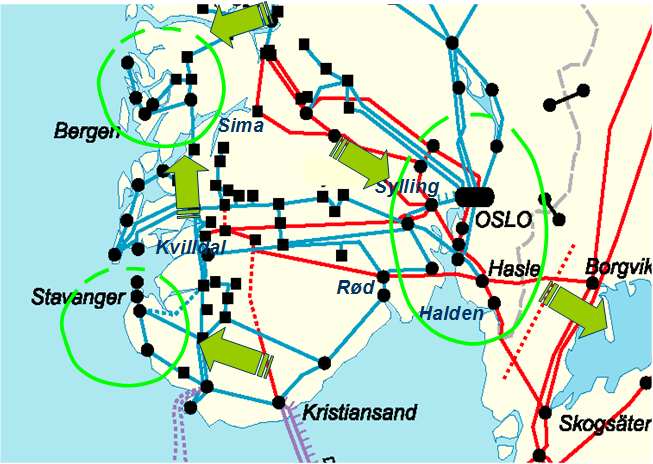
\includegraphics[width=1\textwidth]{Figs/Hasle.png}    
\end{column}
\begin{column}{0.3\textwidth}
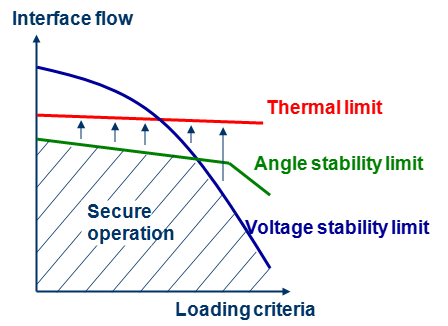
\includegraphics[width=1\textwidth]{Figs/SecurityLimits.png}
\end{column}
\end{columns}  
\end{block}
\begin{block}{Math formulation}
  \begin{align*}
    P_l \leq P_l^{\text{max}}, \; \forall \text{ critical interfaces } l.
  \end{align*}
\underline{Note:} \emph{same math formulation as thermal limits but fundamentally different constraints!}
\end{block}
\end{frame}


\begin{frame}
  \frametitle{Example from Sweden: Using CPF for security management.}
  \begin{columns}
    \column{0.5\textwidth}
    \begin{itemize}
    \item Four price areas separated by bottlenecks (=critical transmission corridors).
    \item \textbf{Security assessment} The TSO monitors the power transfers across the bottlenecks. 
    \item \textbf{Security enhancement} The TSO sends re-dispatch orders (increase/decrease production) if necessary.
    \end{itemize}
    \column{0.5\textwidth}
  \begin{tikzpicture}
\pgftext{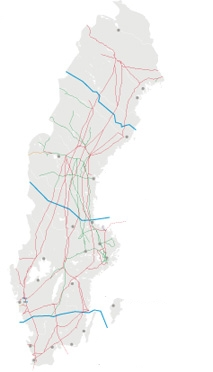
\includegraphics[width=0.55\textwidth]{Figs/Snitten.jpg}}
{\footnotesize
\node at (2.3,2) {Price area SE1};
\node at (1.5,0.25) {Price area SE2};
\node at (1.5,-1.5) {Price area SE3};
\node at (1,-2.5) {Price area SE4};
}
\end{tikzpicture}
  \end{columns}
  \begin{block}{}
What does ``monitoring'' mean in this context? What do we monitor, and against what?
  \end{block}
\end{frame}

\begin{frame}
\frametitle{Example from Sweden - 2}
\begin{columns}
\column{0.6\textwidth}
Security assessment:
\begin{enumerate}
\item A list of contingencies is defined.
\item Every 15 minutes, for each contingency and each bottleneck, transmission limits are computed.
\item The power transfers are monitored and checked against all computed transmission limits.
\end{enumerate}
Security enhancement:
\begin{enumerate}
\setcounter{enumi}{3}
\item If the power transfers come close to one of the computed limits, re-dispatch the generation to decrease the power transfers.
\end{enumerate}
\column{0.4\textwidth}
\begin{center}
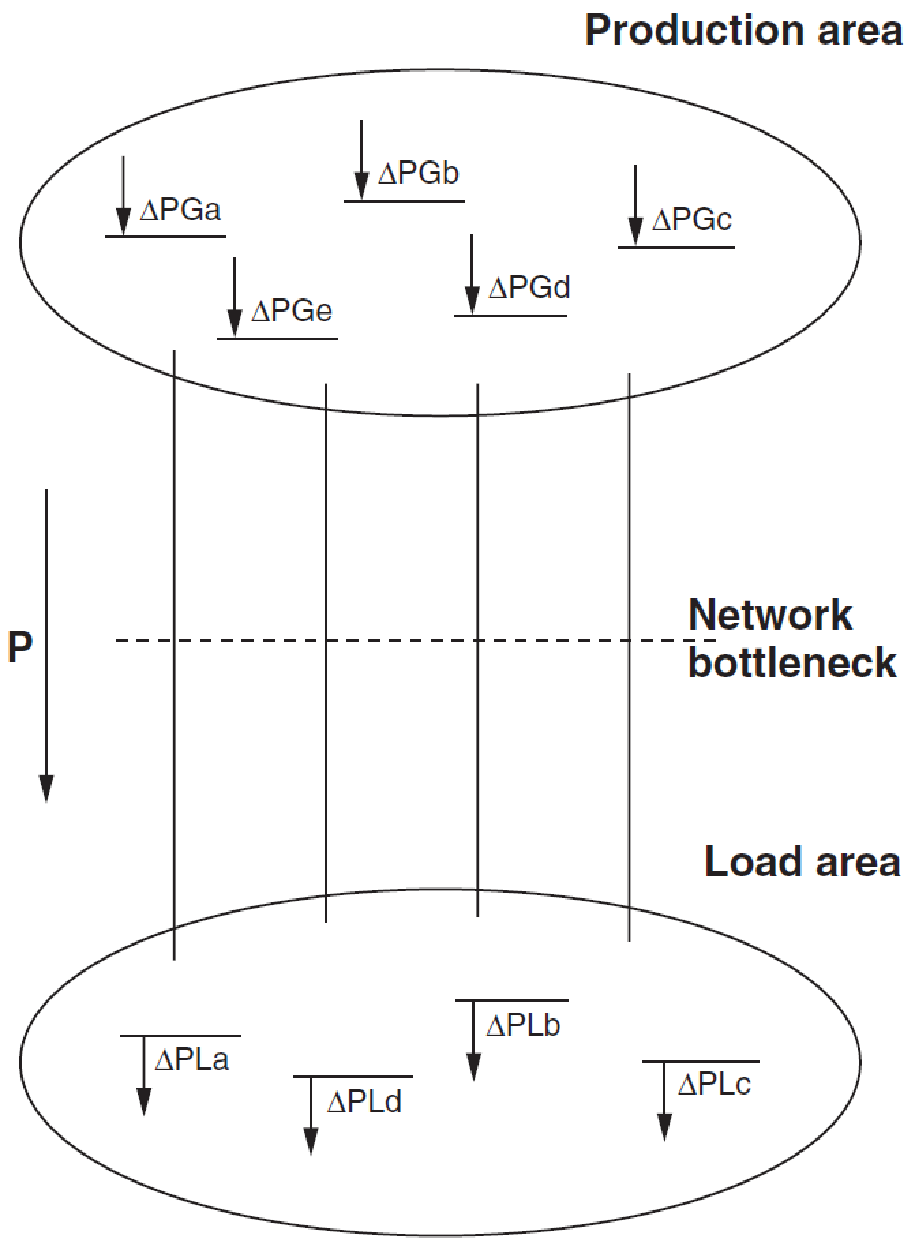
\includegraphics[width=0.85\textwidth]{Figs/SPICAjob}
\end{center}
\end{columns}
\begin{block}{}
How to compute the transmission limits?
\end{block}
\end{frame}

\begin{frame}
\frametitle{Example from Sweden - 3}
\begin{center}
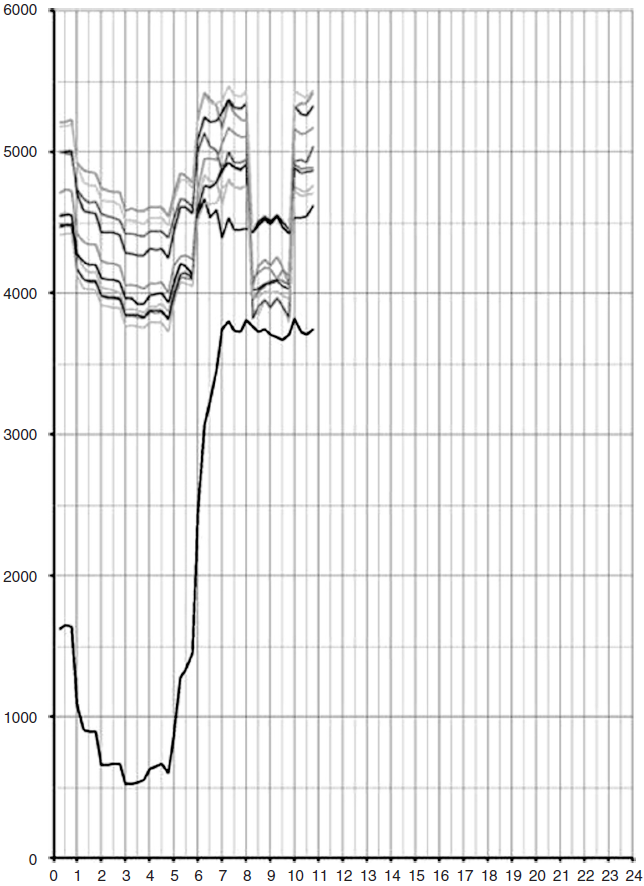
\includegraphics[height=6cm,width=0.75\textwidth]{Figs/SpicaResults.png}

\footnotesize{Source: Sandberg, L., \& Roudén, K. (1992). \textit{The real-time supervision of transmission capacity in the swedish grid}. In S. C. Savulescu (Ed.), \textit{Real-time stability assessment in modern power system control centers}.}
\end{center}
\end{frame}


\begin{frame}[label=example]
\frametitle{Example of voltage instability - 1}
There is a \alert{loading} point beyond which the system becomes unstable.
How to define a \alert{loading} and a \alert{loading increase} in power systems?
\begin{columns}
\column{0.5\textwidth}
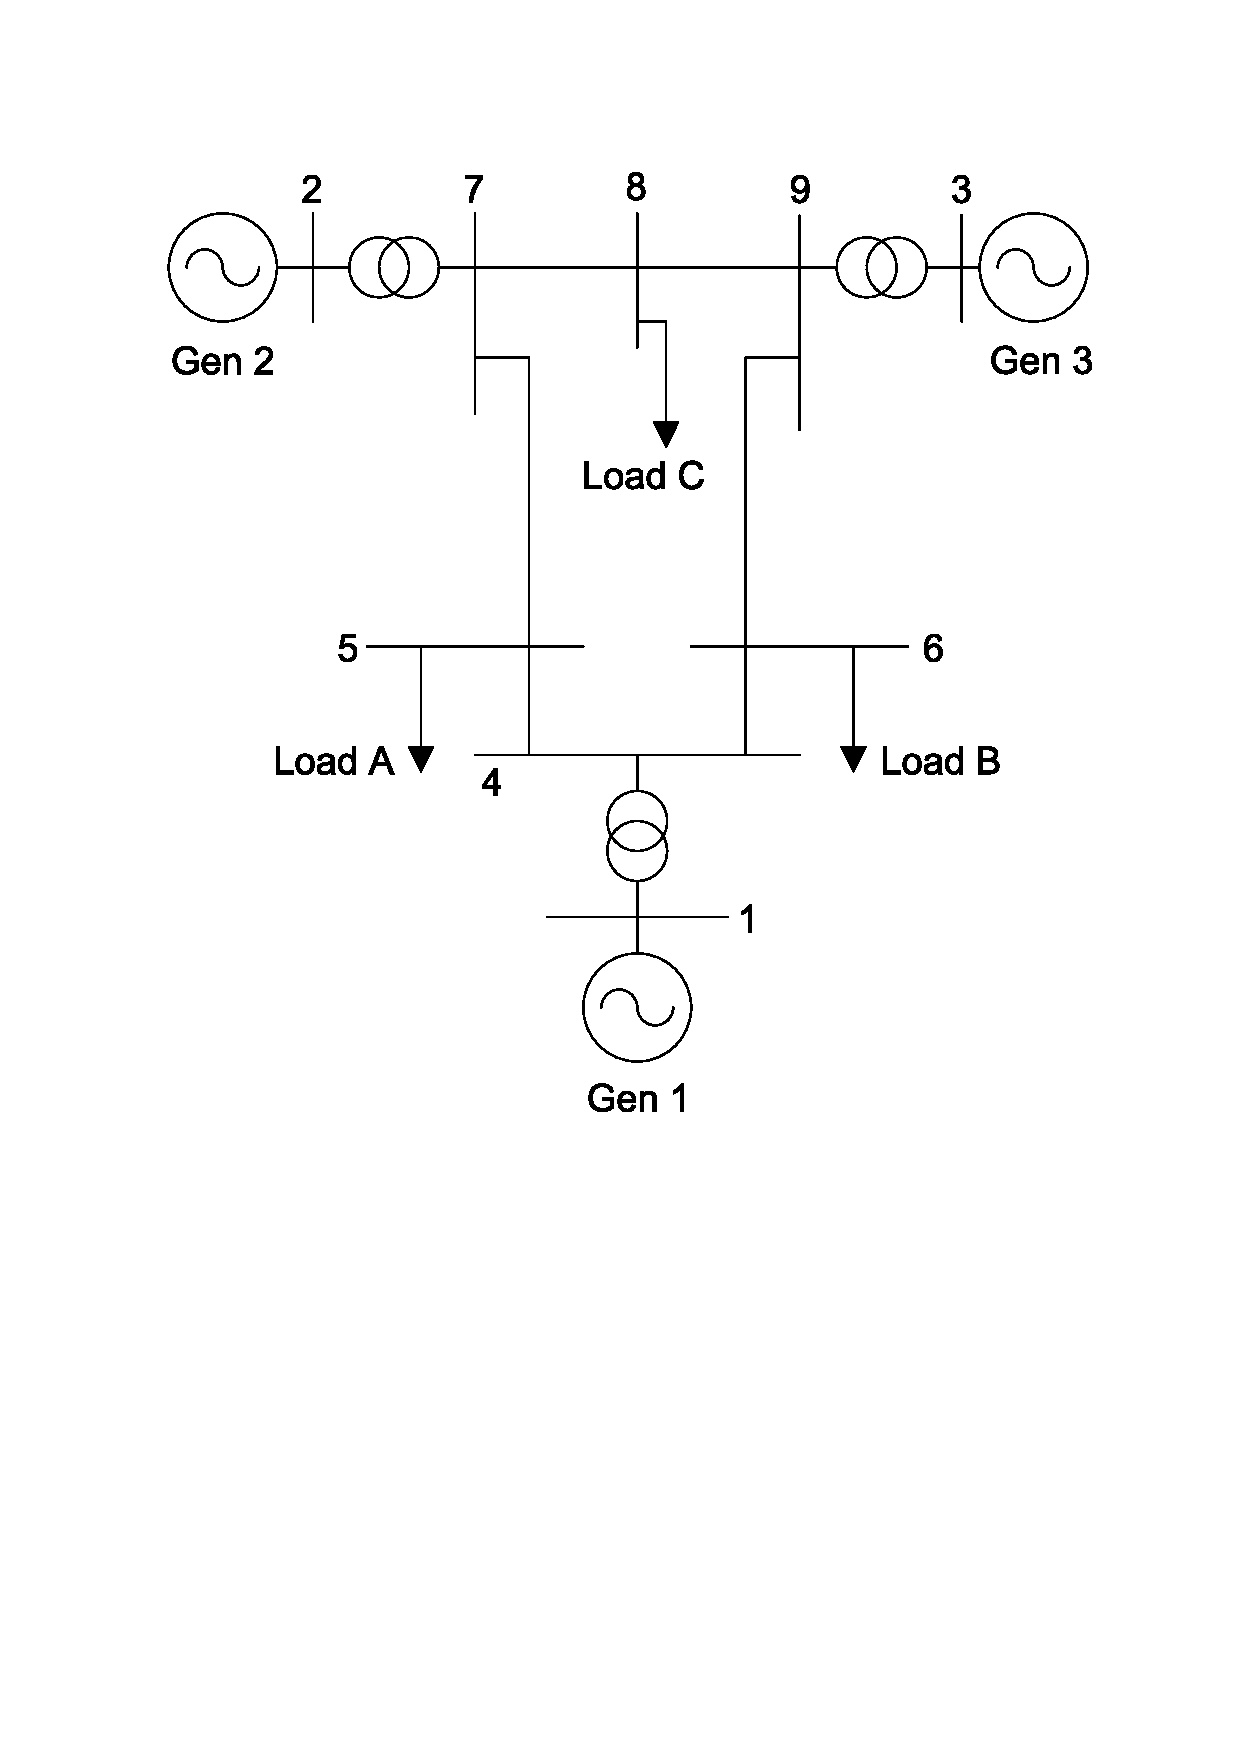
\includegraphics[width=\textwidth]{Figs/Ieee9bus.pdf}
\column{0.5\textwidth}
% This file was created by matlab2tikz v0.4.1.
% Copyright (c) 2008--2013, Nico Schlömer <nico.schloemer@gmail.com>
% All rights reserved.
% 
% The latest updates can be retrieved from
%   http://www.mathworks.com/matlabcentral/fileexchange/22022-matlab2tikz
% where you can also make suggestions and rate matlab2tikz.
% 
% 
% 
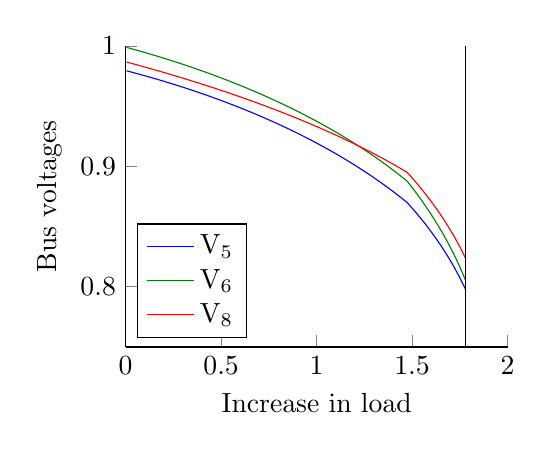
\begin{tikzpicture}

\begin{axis}[%
width=\fwidth,
height=0.788709677419355\fwidth,
scale only axis,
xmin=0,
xmax=2,
xlabel={Increase in load},
ymin=0.75,
ymax=1,
ylabel={Bus voltages},
axis x line*=bottom,
axis y line*=left,
legend style={draw=black,fill=white,legend cell align=left},
legend pos = south west
]
\addplot [
color=blue,
solid
]
table[row sep=crcr]{
0.005 0.979232052476942\\
0.01 0.97902472499685\\
0.015 0.978816627748652\\
0.02 0.978607758936801\\
0.025 0.978398116752672\\
0.03 0.978187699374455\\
0.035 0.977976504967064\\
0.04 0.977764531682033\\
0.045 0.977551777657413\\
0.05 0.977338241017672\\
0.055 0.977123919873591\\
0.06 0.976908812322158\\
0.065 0.976692916446462\\
0.07 0.976476230315584\\
0.075 0.976258751984497\\
0.08 0.97604047949394\\
0.085 0.975821410870326\\
0.09 0.975601544125613\\
0.095 0.975380877257204\\
0.1 0.975159408247819\\
0.105 0.974937135065394\\
0.11 0.974714055662948\\
0.115 0.974490167978475\\
0.12 0.97426546993482\\
0.125 0.974039959439555\\
0.13 0.973813634384864\\
0.135 0.97358649264741\\
0.14 0.973358532088208\\
0.145 0.973129750552511\\
0.15 0.972900145869665\\
0.155 0.972669715852988\\
0.16 0.972438458299638\\
0.165 0.972206370990475\\
0.17 0.971973451689931\\
0.175 0.971739698145868\\
0.18 0.971505108089446\\
0.185 0.971269679234981\\
0.19 0.971033409279799\\
0.195 0.9707962959041\\
0.2 0.970558336770811\\
0.205 0.970319529525434\\
0.21 0.970079871795907\\
0.215 0.969839361192448\\
0.22 0.969597995307403\\
0.225 0.969355771715097\\
0.23 0.96911268797167\\
0.235 0.968868741614931\\
0.24 0.96862393016419\\
0.245 0.968378251120101\\
0.25 0.968131701964495\\
0.255 0.967884280160218\\
0.26 0.967635983150967\\
0.265 0.967386808361114\\
0.27 0.967136753195537\\
0.275 0.966885815039451\\
0.28 0.966633991258225\\
0.285 0.966381279197213\\
0.29 0.966127676181567\\
0.295 0.965873179516057\\
0.3 0.965617786484891\\
0.305 0.965361494351521\\
0.31 0.965104300358459\\
0.315 0.964846201727088\\
0.32 0.964587195657461\\
0.325 0.96432727932811\\
0.33 0.964066449895848\\
0.335 0.963804704495564\\
0.34 0.963542040240023\\
0.345 0.96327845421966\\
0.35 0.963013943502367\\
0.355 0.962748505133287\\
0.36 0.962482136134595\\
0.365 0.962214833505284\\
0.37 0.961946594220946\\
0.375 0.961677415233546\\
0.38 0.9614072934712\\
0.385 0.961136225837946\\
0.39 0.96086420921351\\
0.395 0.960591240453077\\
0.4 0.960317316387048\\
0.405 0.960042433820804\\
0.41 0.959766589534459\\
0.415 0.959489780282617\\
0.42 0.959212002794118\\
0.425 0.958933253771787\\
0.43 0.958653529892179\\
0.435 0.958372827805316\\
0.44 0.958091144134421\\
0.445 0.957808475475659\\
0.45 0.95752481839786\\
0.455 0.957240169442246\\
0.46 0.956954525122153\\
0.465 0.956667881922752\\
0.47 0.956380236300759\\
0.475 0.956091584684149\\
0.48 0.955801923471864\\
0.485 0.955511249033509\\
0.49 0.955219557709055\\
0.495 0.954926845808539\\
0.5 0.954633109611744\\
0.505 0.95433834536789\\
0.51 0.954042549295318\\
0.515 0.953745717581161\\
0.52 0.953447846381022\\
0.525 0.953148931818643\\
0.53 0.952848969985562\\
0.535 0.952547956940778\\
0.54 0.952245888710402\\
0.545 0.951942761287309\\
0.55 0.951638570630777\\
0.555 0.951333312666132\\
0.56 0.951026983284377\\
0.565 0.950719578341824\\
0.57 0.950411093659716\\
0.575 0.950101525023845\\
0.58 0.949790868184165\\
0.585 0.949479118854398\\
0.59 0.949166272711636\\
0.595 0.948852325395935\\
0.6 0.948537272509908\\
0.605 0.948221109618302\\
0.61 0.947903832247581\\
0.615 0.947585435885496\\
0.62 0.947265915980647\\
0.625 0.946945267942044\\
0.63 0.946623487138658\\
0.635 0.946300568898964\\
0.64 0.945976508510484\\
0.645 0.945651301219311\\
0.65 0.945324942229641\\
0.655 0.944997426703284\\
0.66 0.944668749759176\\
0.665 0.944338906472882\\
0.67 0.944007891876088\\
0.675 0.943675700956093\\
0.68 0.943342328655279\\
0.685000000000001 0.943007769870591\\
0.690000000000001 0.942672019452993\\
0.695000000000001 0.94233507220693\\
0.700000000000001 0.941996922889765\\
0.705000000000001 0.941657566211222\\
0.710000000000001 0.941316996832811\\
0.715000000000001 0.940975209367252\\
0.720000000000001 0.94063219837788\\
0.725000000000001 0.940287958378049\\
0.730000000000001 0.939942483830522\\
0.735000000000001 0.939595769146855\\
0.740000000000001 0.939247808686765\\
0.745000000000001 0.938898596757493\\
0.750000000000001 0.938548127613157\\
0.755000000000001 0.938196395454092\\
0.760000000000001 0.937843394426179\\
0.765000000000001 0.937489118620167\\
0.770000000000001 0.937133562070975\\
0.775000000000001 0.936776718756997\\
0.780000000000001 0.93641858259938\\
0.785000000000001 0.936059147461303\\
0.790000000000001 0.935698407147235\\
0.795000000000001 0.935336355402183\\
0.800000000000001 0.934972985910932\\
0.805000000000001 0.934608292297266\\
0.810000000000001 0.93424226812318\\
0.815000000000001 0.933874906888075\\
0.820000000000001 0.933506202027946\\
0.825000000000001 0.933136146914546\\
0.830000000000001 0.932764734854547\\
0.835000000000001 0.932391959088675\\
0.840000000000001 0.932017812790845\\
0.845000000000001 0.931642289067262\\
0.850000000000001 0.931265380955526\\
0.855000000000001 0.930887081423705\\
0.860000000000001 0.930507383369403\\
0.865000000000001 0.930126279618808\\
0.870000000000001 0.929743762925718\\
0.875000000000001 0.929359825970559\\
0.880000000000001 0.928974461359383\\
0.885000000000001 0.928587661622839\\
0.890000000000001 0.928199419215138\\
0.895000000000001 0.927809726512996\\
0.900000000000001 0.927418575814553\\
0.905000000000001 0.927025959338274\\
0.910000000000001 0.926631869221839\\
0.915000000000001 0.926236297520995\\
0.920000000000001 0.925839236208407\\
0.925000000000001 0.925440677172475\\
0.930000000000001 0.925040612216129\\
0.935000000000001 0.924639033055613\\
0.940000000000001 0.924235931319227\\
0.945000000000001 0.923831298546071\\
0.950000000000001 0.923425126184737\\
0.955000000000001 0.923017405592005\\
0.960000000000001 0.922608128031487\\
0.965000000000001 0.922197284672269\\
0.970000000000001 0.921784866587509\\
0.975000000000001 0.921370864753017\\
0.980000000000001 0.920955270045811\\
0.985000000000001 0.920538073242635\\
0.990000000000001 0.920119265018455\\
0.995000000000001 0.919698835944925\\
1 0.919276776488821\\
1.005 0.918853077010446\\
1.01 0.918427727762004\\
1.015 0.91800071888594\\
1.02 0.917572040413243\\
1.025 0.917141682261728\\
1.03 0.916709634234268\\
1.035 0.916275886017003\\
1.04 0.9158404271775\\
1.045 0.915403247162889\\
1.05 0.914964335297953\\
1.055 0.914523680783177\\
1.06 0.914081272692762\\
1.065 0.913637099972596\\
1.07 0.913191151438185\\
1.075 0.912743415772529\\
1.08 0.912293881523976\\
1.085 0.911842537104001\\
1.09 0.911389370784969\\
1.095 0.910934370697825\\
1.1 0.91047752482975\\
1.105 0.910018821021757\\
1.11 0.909558246966245\\
1.115 0.909095790204486\\
1.12 0.908631438124073\\
1.125 0.908165177956298\\
1.13 0.907696996773481\\
1.135 0.907226881486238\\
1.14 0.906754818840685\\
1.145 0.906280795415581\\
1.15 0.90580479761941\\
1.155 0.905326811687392\\
1.16 0.904846823678429\\
1.165 0.90436481947198\\
1.17 0.903880784764868\\
1.175 0.903394705068004\\
1.18 0.902906565703046\\
1.185 0.902416351798974\\
1.19 0.901924048288587\\
1.195 0.901429639904913\\
1.2 0.900933111177543\\
1.20497298395187 0.900437146584785\\
1.20992526856465 0.899941131037016\\
1.21485696063708 0.899445064689713\\
1.21976816591341 0.898948947696048\\
1.22465898907991 0.898452780206842\\
1.22952953378013 0.897956562370589\\
1.23437990262991 0.897460294333487\\
1.23921019723211 0.896963976239474\\
1.2440205181911 0.896467608230245\\
1.24881096512691 0.895971190445292\\
1.25358163668918 0.895474723021924\\
1.25833263057079 0.894978206095298\\
1.26306404352137 0.894481639798445\\
1.26777597136041 0.893985024262295\\
1.27246850899021 0.893488359615704\\
1.27714175040859 0.89299164598548\\
1.28179578872141 0.892494883496404\\
1.28643071615476 0.89199807227126\\
1.29104662406705 0.891501212430853\\
1.29564360296083 0.891004304094036\\
1.30022174249439 0.890507347377731\\
1.30478113149316 0.890010342396953\\
1.30932185796096 0.889513289264831\\
1.31384400909099 0.88901618809263\\
1.31834767127666 0.888519038989772\\
1.32283293012223 0.888021842063856\\
1.32729987045327 0.887524597420682\\
1.33174857632692 0.887027305164266\\
1.336179131042 0.886529965396862\\
1.34059161714895 0.886032578218982\\
1.34498611645954 0.885535143729415\\
1.34936271005653 0.885037662025244\\
1.35372147830306 0.884540133201866\\
1.35806250085191 0.884042557353006\\
1.36238585665466 0.883544934570742\\
1.36669162397063 0.883047264945515\\
1.37097988037572 0.88254954856615\\
1.37525070277103 0.882051785519872\\
1.37950416739145 0.881553975892319\\
1.38374034981404 0.881056119767564\\
1.38795932496622 0.880558217228126\\
1.39216116713397 0.880060268354987\\
1.39634594996977 0.879562273227608\\
1.40051374650046 0.879064231923942\\
1.40466462913498 0.87856614452045\\
1.40879866967199 0.878068011092116\\
1.41291593930731 0.877569831712458\\
1.41701650864131 0.877071606453547\\
1.4211004476862 0.876573335386014\\
1.4251678258731 0.876075018579069\\
1.42921871205906 0.875576656100512\\
1.43325317453404 0.875078248016746\\
1.43727128102765 0.874579794392787\\
1.44127309871588 0.874081295292283\\
1.44525869422766 0.873582750777517\\
1.44922813365137 0.873084160909429\\
1.45318148254125 0.87258552574762\\
1.45711880592367 0.872086845350366\\
1.4610401683033 0.87158811977463\\
1.46494563366927 0.871089349076074\\
1.46883526550114 0.870590533309067\\
1.47270912677483 0.870091672526697\\
1.47579130221616 0.869628004653946\\
1.47829399300274 0.869190161405018\\
1.48078768860855 0.868752308829099\\
1.48327241224409 0.868314447007678\\
1.48574818699804 0.867876576022114\\
1.48821503583894 0.867438695953651\\
1.49067298161619 0.867000806883415\\
1.49312204706092 0.866562908892419\\
1.4955622547869 0.866125002061569\\
1.49799362729146 0.865687086471663\\
1.50041618695643 0.865249162203397\\
1.50282995604894 0.864811229337368\\
1.50523495672237 0.864373287954076\\
1.50763121101719 0.86393533813393\\
1.51001874086183 0.863497379957246\\
1.51239756807352 0.863059413504256\\
1.51476771435915 0.86262143885511\\
1.51712920131609 0.862183456089875\\
1.51948205043304 0.861745465288542\\
1.52182628309083 0.861307466531028\\
1.52416192056321 0.860869459897181\\
1.52648898401772 0.860431445466779\\
1.52880749451639 0.859993423319538\\
1.53111747301665 0.85955539353511\\
1.53341894037198 0.859117356193091\\
1.53571191733276 0.858679311373022\\
1.53799642454702 0.858241259154388\\
1.54027248256119 0.85780319961663\\
1.54254011182085 0.85736513283914\\
1.54479933267149 0.856927058901266\\
1.54705016535919 0.856488977882318\\
1.54929263003143 0.856050889861569\\
1.55152674673775 0.855612794918257\\
1.55375253543047 0.855174693131589\\
1.55597001596542 0.854736584580744\\
1.55817920810264 0.854298469344875\\
1.56038013150704 0.853860347503114\\
1.56257280574913 0.853422219134572\\
1.56475725030568 0.852984084318346\\
1.56693348456037 0.852545943133518\\
1.5691015278045 0.852107795659158\\
1.57126139923764 0.851669641974332\\
1.57341311796827 0.851231482158099\\
1.57555670301444 0.850793316289514\\
1.5776921733044 0.850355144447637\\
1.57981954767726 0.84991696671153\\
1.58193884488359 0.84947878316026\\
1.5840500835861 0.849040593872908\\
1.58615328236017 0.848602398928562\\
1.58824845969456 0.84816419840633\\
1.59033563399195 0.847725992385334\\
1.59241482356956 0.84728778094472\\
1.59448604665977 0.846849564163657\\
1.59654932141069 0.846411342121339\\
1.59860466588672 0.845973114896991\\
1.60065209806919 0.845534882569871\\
1.6026916358569 0.845096645219269\\
1.60472329706666 0.844658402924514\\
1.60674709943393 0.844220155764978\\
1.60876306061331 0.843781903820073\\
1.61077119817912 0.843343647169259\\
1.61277152962596 0.842905385892045\\
1.61476407236924 0.842467120067991\\
1.61674884374571 0.842028849776711\\
1.61872586101402 0.841590575097877\\
1.62069514135523 0.841152296111222\\
1.62265670187335 0.840714012896541\\
1.62461055959583 0.840275725533693\\
1.62655673147413 0.839837434102608\\
1.62849523438416 0.839399138683286\\
1.63042608512686 0.8389608393558\\
1.63234930042862 0.8385225362003\\
1.63426489694185 0.838084229297017\\
1.63617289124547 0.837645918726263\\
1.63807329984532 0.837207604568434\\
1.63996613917473 0.836769286904015\\
1.64185142559497 0.836330965813581\\
1.64372917539571 0.8358926413778\\
1.6455994047955 0.835454313677436\\
1.64746212994226 0.835015982793352\\
1.64931736691372 0.834577648806512\\
1.65116513171786 0.834139311797985\\
1.65300544029344 0.833700971848945\\
1.65483830851035 0.833262629040678\\
1.65666375217014 0.832824283454581\\
1.65848178700643 0.832385935172168\\
1.66029242868532 0.831947584275069\\
1.6620956928059 0.831509230845035\\
1.66389159490061 0.831070874963942\\
1.66568015043572 0.830632516713791\\
1.6674613748117 0.830194156176713\\
1.6692352833637 0.82975579343497\\
1.67100189136193 0.829317428570958\\
1.67276121401209 0.828879061667212\\
1.67451326645577 0.828440692806407\\
1.67625806377087 0.82800232207136\\
1.67799562097198 0.827563949545034\\
1.6797259530108 0.827125575310542\\
1.68144907477654 0.826687199451146\\
1.68316500109629 0.826248822050264\\
1.68487374673544 0.82581044319147\\
1.68657532639803 0.825372062958497\\
1.68826975472718 0.824933681435243\\
1.68995704630543 0.82449529870577\\
1.69163721565512 0.824056914854306\\
1.69331027723879 0.823618529965256\\
1.69497624545954 0.823180144123192\\
1.69663513466137 0.822741757412867\\
1.69828695912959 0.822303369919213\\
1.69993173309116 0.821864981727342\\
1.70156947071501 0.821426592922556\\
1.70320018611249 0.82098820359034\\
1.70482389333761 0.820549813816373\\
1.70644060638749 0.820111423686527\\
1.70805033920263 0.819673033286871\\
1.70965310566729 0.819234642703675\\
1.71124891960986 0.818796252023408\\
1.7128377948031 0.818357861332748\\
1.71441974496461 0.81791947071858\\
1.71599478375704 0.817481080267999\\
1.71756292478849 0.817042690068318\\
1.71912418161284 0.816604300207063\\
1.72067856773003 0.816165910771982\\
1.7222260965864 0.815727521851048\\
1.72376678157505 0.815289133532456\\
1.72530063603609 0.814850745904633\\
1.726827673257 0.814412359056236\\
1.72834790647294 0.81397397307616\\
1.72986134886702 0.813535588053534\\
1.73136801357067 0.813097204077732\\
1.73286791366386 0.812658821238369\\
1.73436106217552 0.812220439625308\\
1.7358474720837 0.811782059328663\\
1.73732715631597 0.8113436804388\\
1.73880012774968 0.810905303046343\\
1.74026639921226 0.810466927242172\\
1.7417259834815 0.810028553117432\\
1.74317889328582 0.809590180763534\\
1.7446251413046 0.809151810272155\\
1.74606474016843 0.808713441735246\\
1.7474977024594 0.808275075245032\\
1.74892404071139 0.807836710894016\\
1.75034376741033 0.807398348774981\\
1.75175689499446 0.806959988980998\\
1.75316343585465 0.80652163160542\\
1.75456340233463 0.806083276741896\\
1.75595680673126 0.805644924484365\\
1.75734366129481 0.805206574927065\\
1.75872397822922 0.804768228164535\\
1.76009776969238 0.804329884291616\\
1.76146504779632 0.803891543403457\\
1.76282582460756 0.803453205595516\\
1.76418011214731 0.803014870963566\\
1.76552792239173 0.802576539603695\\
1.76686926727219 0.802138211612313\\
1.76820415867552 0.801699887086152\\
1.76953260844424 0.801261566122271\\
1.77085462837683 0.80082324881806\\
1.77217023022798 0.800384935271242\\
1.77347942570878 0.799946625579877\\
1.77478222648702 0.799508319842363\\
1.7760786441874 0.799070018157447\\
1.77736869039176 0.798631720624219\\
1.77865237663933 0.798193427342121\\
1.77992971442697 0.797755138410948\\
1.78120071520936 0.797316853930855\\
};
\addlegendentry{$\text{V}_\text{5}$};

\addplot [
color=green!50!black,
solid
]
table[row sep=crcr]{
0.005 0.998686038128165\\
0.01 0.998470807513519\\
0.015 0.998254815896074\\
0.02 0.998038061500132\\
0.025 0.997820542537159\\
0.03 0.997602257205685\\
0.035 0.997383203691213\\
0.04 0.997163380166114\\
0.045 0.996942784789531\\
0.05 0.996721415707276\\
0.055 0.996499271051735\\
0.06 0.996276348941757\\
0.065 0.996052647482554\\
0.07 0.995828164765599\\
0.075 0.995602898868513\\
0.08 0.995376847854963\\
0.085 0.995150009774552\\
0.09 0.994922382662708\\
0.095 0.994693964540574\\
0.1 0.994464753414892\\
0.105 0.9942347472779\\
0.11 0.994003944107203\\
0.115 0.993772341865665\\
0.12 0.993539938501291\\
0.125 0.993306731947106\\
0.13 0.993072720121036\\
0.135 0.992837900925786\\
0.14 0.992602272248714\\
0.145 0.992365831961713\\
0.15 0.992128577921079\\
0.155 0.991890507967386\\
0.16 0.991651619925355\\
0.165 0.99141191160373\\
0.17 0.991171380795137\\
0.175 0.990930025275956\\
0.18 0.990687842806186\\
0.185 0.990444831129306\\
0.19 0.990200987972138\\
0.195 0.989956311044708\\
0.2 0.989710798040102\\
0.205 0.989464446634324\\
0.21 0.989217254486153\\
0.215 0.988969219236992\\
0.22 0.988720338510728\\
0.225 0.988470609913568\\
0.23 0.9882200310339\\
0.235 0.987968599442133\\
0.24 0.987716312690542\\
0.245 0.987463168313114\\
0.25 0.987209163825381\\
0.255 0.986954296724267\\
0.26 0.98669856448792\\
0.265 0.986441964575546\\
0.27 0.986184494427244\\
0.275 0.985926151463838\\
0.28 0.9856669330867\\
0.285 0.985406836677582\\
0.29 0.985145859598439\\
0.295 0.984883999191248\\
0.3 0.984621252777832\\
0.305 0.984357617659675\\
0.31 0.98409309111774\\
0.315 0.983827670412279\\
0.32 0.983561352782646\\
0.325 0.983294135447103\\
0.33 0.983026015602632\\
0.335 0.982756990424732\\
0.34 0.982487057067221\\
0.345 0.982216212662041\\
0.35 0.981944454319044\\
0.355 0.981671779125794\\
0.36 0.981398184147355\\
0.365 0.981123666426076\\
0.37 0.980848222981382\\
0.375 0.980571850809553\\
0.38 0.980294546883505\\
0.385 0.980016308152566\\
0.39 0.979737131542254\\
0.395 0.979457013954042\\
0.4 0.979175952265133\\
0.405 0.97889394332822\\
0.41 0.978610983971251\\
0.415 0.978327070997188\\
0.42 0.978042201183761\\
0.425 0.977756371283223\\
0.43 0.977469578022098\\
0.435 0.97718181810093\\
0.44 0.976893088194018\\
0.445 0.976603384949168\\
0.45 0.976312704987417\\
0.455 0.97602104490277\\
0.46 0.975728401261932\\
0.465 0.975434770604026\\
0.47 0.975140149440322\\
0.475 0.974844534253947\\
0.48 0.974547921499608\\
0.485 0.97425030760329\\
0.49 0.973951688961974\\
0.495 0.973652061943331\\
0.5 0.973351422885422\\
0.505 0.973049768096394\\
0.51 0.972747093854166\\
0.515 0.972443396406114\\
0.52 0.972138671968755\\
0.525 0.971832916727424\\
0.53 0.971526126835937\\
0.535 0.971218298416271\\
0.54 0.970909427558217\\
0.545 0.97059951031904\\
0.55 0.970288542723136\\
0.555 0.969976520761674\\
0.56 0.969663440392244\\
0.565 0.96934929753849\\
0.57 0.96903408808975\\
0.575 0.968717807900674\\
0.58 0.968400452790854\\
0.585 0.968082018544437\\
0.59 0.967762500909739\\
0.595 0.967441895598846\\
0.6 0.967120198287216\\
0.605 0.966797404613275\\
0.61 0.966473510178001\\
0.615 0.966148510544509\\
0.62 0.965822401237626\\
0.625 0.965495177743459\\
0.63 0.965166835508959\\
0.635 0.964837369941478\\
0.64 0.964506776408318\\
0.645 0.964175050236276\\
0.65 0.963842186711176\\
0.655 0.963508181077405\\
0.66 0.963173028537426\\
0.665 0.962836724251306\\
0.67 0.962499263336208\\
0.675 0.962160640865904\\
0.68 0.96182085187026\\
0.685000000000001 0.961479891334724\\
0.690000000000001 0.961137754199798\\
0.695000000000001 0.960794435360515\\
0.700000000000001 0.96044992966589\\
0.705000000000001 0.960104231918377\\
0.710000000000001 0.959757336873312\\
0.715000000000001 0.959409239238344\\
0.720000000000001 0.959059933672865\\
0.725000000000001 0.958709414787425\\
0.730000000000001 0.958357677143137\\
0.735000000000001 0.95800471525108\\
0.740000000000001 0.957650523571678\\
0.745000000000001 0.95729509651409\\
0.750000000000001 0.95693842843557\\
0.755000000000001 0.956580513640829\\
0.760000000000001 0.95622134638138\\
0.765000000000001 0.955860920854878\\
0.770000000000001 0.955499231204446\\
0.775000000000001 0.955136271517989\\
0.780000000000001 0.954772035827498\\
0.785000000000001 0.954406518108345\\
0.790000000000001 0.954039712278562\\
0.795000000000001 0.95367161219811\\
0.800000000000001 0.953302211668138\\
0.805000000000001 0.952931504430224\\
0.810000000000001 0.952559484165609\\
0.815000000000001 0.952186144494416\\
0.820000000000001 0.951811478974857\\
0.825000000000001 0.951435481102418\\
0.830000000000001 0.951058144309046\\
0.835000000000001 0.95067946196231\\
0.840000000000001 0.950299427364549\\
0.845000000000001 0.949918033752009\\
0.850000000000001 0.949535274293966\\
0.855000000000001 0.949151142091824\\
0.860000000000001 0.948765630178213\\
0.865000000000001 0.948378731516058\\
0.870000000000001 0.947990438997632\\
0.875000000000001 0.947600745443607\\
0.880000000000001 0.94720964360207\\
0.885000000000001 0.946817126147532\\
0.890000000000001 0.946423185679912\\
0.895000000000001 0.946027814723517\\
0.900000000000001 0.945631005725988\\
0.905000000000001 0.945232751057228\\
0.910000000000001 0.944833043008327\\
0.915000000000001 0.944431873790448\\
0.920000000000001 0.944029235533704\\
0.925000000000001 0.943625120286008\\
0.930000000000001 0.943219520011909\\
0.935000000000001 0.9428124265914\\
0.940000000000001 0.942403831818708\\
0.945000000000001 0.941993727401055\\
0.950000000000001 0.941582104957407\\
0.955000000000001 0.941168956017191\\
0.960000000000001 0.940754272018985\\
0.965000000000001 0.940338044309195\\
0.970000000000001 0.939920264140697\\
0.975000000000001 0.93950092267145\\
0.980000000000001 0.939080010963102\\
0.985000000000001 0.93865751997954\\
0.990000000000001 0.938233440585439\\
0.995000000000001 0.937807763544761\\
1 0.937380479519245\\
1.005 0.936951579066849\\
1.01 0.936521052640174\\
1.015 0.93608889058485\\
1.02 0.935655083137893\\
1.025 0.935219620426027\\
1.03 0.934782492463977\\
1.035 0.93434368915272\\
1.04 0.933903200277709\\
1.045 0.933461015507054\\
1.05 0.933017124389671\\
1.055 0.932571516353387\\
1.06 0.932124180703016\\
1.065 0.931675106618382\\
1.07 0.931224283152313\\
1.075 0.930771699228586\\
1.08 0.93031734363983\\
1.085 0.929861205045387\\
1.09 0.929403271969127\\
1.095 0.928943532797212\\
1.1 0.928481975775821\\
1.105 0.928018589008819\\
1.11 0.927553360455379\\
1.115 0.927086277927544\\
1.12 0.926617329087758\\
1.125 0.926146501446313\\
1.13 0.925673782358763\\
1.135 0.925199159023272\\
1.14 0.924722618477902\\
1.145 0.924244147597843\\
1.15 0.923763733092579\\
1.155 0.923281361502994\\
1.16 0.922797019198407\\
1.165 0.922310692373541\\
1.17 0.92182236704543\\
1.175 0.921332029050237\\
1.18 0.920839664040022\\
1.185 0.920345257479411\\
1.19 0.919848794642212\\
1.195 0.919350260607925\\
1.2 0.918849640258189\\
1.20497298395187 0.918349640258189\\
1.20992526856465 0.917849640258189\\
1.21485696063708 0.91734964025819\\
1.21976816591341 0.91684964025819\\
1.22465898907991 0.91634964025819\\
1.22952953378013 0.91584964025819\\
1.23437990262991 0.91534964025819\\
1.23921019723211 0.91484964025819\\
1.2440205181911 0.91434964025819\\
1.24881096512691 0.91384964025819\\
1.25358163668918 0.91334964025819\\
1.25833263057079 0.912849640258191\\
1.26306404352137 0.912349640258191\\
1.26777597136041 0.911849640258191\\
1.27246850899021 0.911349640258191\\
1.27714175040859 0.910849640258191\\
1.28179578872141 0.910349640258191\\
1.28643071615476 0.909849640258191\\
1.29104662406705 0.909349640258191\\
1.29564360296083 0.908849640258191\\
1.30022174249439 0.908349640258191\\
1.30478113149316 0.907849640258192\\
1.30932185796096 0.907349640258192\\
1.31384400909099 0.906849640258192\\
1.31834767127666 0.906349640258192\\
1.32283293012223 0.905849640258192\\
1.32729987045327 0.905349640258192\\
1.33174857632692 0.904849640258192\\
1.336179131042 0.904349640258192\\
1.34059161714895 0.903849640258192\\
1.34498611645954 0.903349640258192\\
1.34936271005653 0.902849640258192\\
1.35372147830306 0.902349640258192\\
1.35806250085191 0.901849640258192\\
1.36238585665466 0.901349640258192\\
1.36669162397063 0.900849640258192\\
1.37097988037572 0.900349640258192\\
1.37525070277103 0.899849640258192\\
1.37950416739145 0.899349640258192\\
1.38374034981404 0.898849640258192\\
1.38795932496622 0.898349640258192\\
1.39216116713397 0.897849640258192\\
1.39634594996977 0.897349640258193\\
1.40051374650046 0.896849640258193\\
1.40466462913498 0.896349640258193\\
1.40879866967199 0.895849640258193\\
1.41291593930731 0.895349640258193\\
1.41701650864131 0.894849640258193\\
1.4211004476862 0.894349640258193\\
1.4251678258731 0.893849640258193\\
1.42921871205906 0.893349640258193\\
1.43325317453404 0.892849640258193\\
1.43727128102765 0.892349640258193\\
1.44127309871588 0.891849640258193\\
1.44525869422766 0.891349640258193\\
1.44922813365137 0.890849640258193\\
1.45318148254125 0.890349640258193\\
1.45711880592367 0.889849640258193\\
1.4610401683033 0.889349640258193\\
1.46494563366927 0.888849640258193\\
1.46883526550114 0.888349640258193\\
1.47270912677483 0.887849640258193\\
1.47579130221616 0.887349640258193\\
1.47829399300274 0.886849640258193\\
1.48078768860855 0.886349640258193\\
1.48327241224409 0.885849640258193\\
1.48574818699804 0.885349640258193\\
1.48821503583894 0.884849640258193\\
1.49067298161619 0.884349640258194\\
1.49312204706092 0.883849640258194\\
1.4955622547869 0.883349640258194\\
1.49799362729146 0.882849640258194\\
1.50041618695643 0.882349640258194\\
1.50282995604894 0.881849640258194\\
1.50523495672237 0.881349640258194\\
1.50763121101719 0.880849640258194\\
1.51001874086183 0.880349640258194\\
1.51239756807352 0.879849640258194\\
1.51476771435915 0.879349640258194\\
1.51712920131609 0.878849640258194\\
1.51948205043304 0.878349640258194\\
1.52182628309083 0.877849640258194\\
1.52416192056321 0.877349640258195\\
1.52648898401772 0.876849640258195\\
1.52880749451639 0.876349640258195\\
1.53111747301665 0.875849640258195\\
1.53341894037198 0.875349640258195\\
1.53571191733276 0.874849640258195\\
1.53799642454702 0.874349640258195\\
1.54027248256119 0.873849640258195\\
1.54254011182085 0.873349640258195\\
1.54479933267149 0.872849640258195\\
1.54705016535919 0.872349640258195\\
1.54929263003143 0.871849640258195\\
1.55152674673775 0.871349640258196\\
1.55375253543047 0.870849640258195\\
1.55597001596542 0.870349640258196\\
1.55817920810264 0.869849640258196\\
1.56038013150704 0.869349640258196\\
1.56257280574913 0.868849640258196\\
1.56475725030568 0.868349640258196\\
1.56693348456037 0.867849640258196\\
1.5691015278045 0.867349640258196\\
1.57126139923764 0.866849640258196\\
1.57341311796827 0.866349640258196\\
1.57555670301444 0.865849640258196\\
1.5776921733044 0.865349640258196\\
1.57981954767726 0.864849640258196\\
1.58193884488359 0.864349640258196\\
1.5840500835861 0.863849640258196\\
1.58615328236017 0.863349640258196\\
1.58824845969456 0.862849640258197\\
1.59033563399195 0.862349640258197\\
1.59241482356956 0.861849640258197\\
1.59448604665977 0.861349640258197\\
1.59654932141069 0.860849640258197\\
1.59860466588672 0.860349640258197\\
1.60065209806919 0.859849640258197\\
1.6026916358569 0.859349640258197\\
1.60472329706666 0.858849640258197\\
1.60674709943393 0.858349640258197\\
1.60876306061331 0.857849640258197\\
1.61077119817912 0.857349640258197\\
1.61277152962596 0.856849640258197\\
1.61476407236924 0.856349640258197\\
1.61674884374571 0.855849640258197\\
1.61872586101402 0.855349640258197\\
1.62069514135523 0.854849640258197\\
1.62265670187335 0.854349640258197\\
1.62461055959583 0.853849640258198\\
1.62655673147413 0.853349640258198\\
1.62849523438416 0.852849640258198\\
1.63042608512686 0.852349640258198\\
1.63234930042862 0.851849640258198\\
1.63426489694185 0.851349640258198\\
1.63617289124547 0.850849640258198\\
1.63807329984532 0.850349640258198\\
1.63996613917473 0.849849640258198\\
1.64185142559497 0.849349640258198\\
1.64372917539571 0.848849640258198\\
1.6455994047955 0.848349640258198\\
1.64746212994226 0.847849640258198\\
1.64931736691372 0.847349640258198\\
1.65116513171786 0.846849640258198\\
1.65300544029344 0.846349640258198\\
1.65483830851035 0.845849640258198\\
1.65666375217014 0.845349640258198\\
1.65848178700643 0.844849640258199\\
1.66029242868532 0.844349640258199\\
1.6620956928059 0.843849640258199\\
1.66389159490061 0.843349640258199\\
1.66568015043572 0.842849640258199\\
1.6674613748117 0.842349640258199\\
1.6692352833637 0.841849640258199\\
1.67100189136193 0.841349640258199\\
1.67276121401209 0.840849640258199\\
1.67451326645577 0.840349640258199\\
1.67625806377087 0.8398496402582\\
1.67799562097198 0.8393496402582\\
1.6797259530108 0.8388496402582\\
1.68144907477654 0.8383496402582\\
1.68316500109629 0.8378496402582\\
1.68487374673544 0.8373496402582\\
1.68657532639803 0.8368496402582\\
1.68826975472718 0.8363496402582\\
1.68995704630543 0.8358496402582\\
1.69163721565512 0.8353496402582\\
1.69331027723879 0.8348496402582\\
1.69497624545954 0.8343496402582\\
1.69663513466137 0.8338496402582\\
1.69828695912959 0.8333496402582\\
1.69993173309116 0.8328496402582\\
1.70156947071501 0.8323496402582\\
1.70320018611249 0.8318496402582\\
1.70482389333761 0.8313496402582\\
1.70644060638749 0.8308496402582\\
1.70805033920263 0.8303496402582\\
1.70965310566729 0.8298496402582\\
1.71124891960986 0.8293496402582\\
1.7128377948031 0.828849640258201\\
1.71441974496461 0.828349640258201\\
1.71599478375704 0.827849640258201\\
1.71756292478849 0.827349640258201\\
1.71912418161284 0.826849640258201\\
1.72067856773003 0.826349640258201\\
1.7222260965864 0.825849640258201\\
1.72376678157505 0.825349640258201\\
1.72530063603609 0.824849640258201\\
1.726827673257 0.824349640258201\\
1.72834790647294 0.823849640258201\\
1.72986134886702 0.823349640258201\\
1.73136801357067 0.822849640258201\\
1.73286791366386 0.822349640258201\\
1.73436106217552 0.821849640258201\\
1.7358474720837 0.821349640258201\\
1.73732715631597 0.820849640258201\\
1.73880012774968 0.820349640258201\\
1.74026639921226 0.819849640258201\\
1.7417259834815 0.819349640258201\\
1.74317889328582 0.818849640258202\\
1.7446251413046 0.818349640258202\\
1.74606474016843 0.817849640258202\\
1.7474977024594 0.817349640258202\\
1.74892404071139 0.816849640258202\\
1.75034376741033 0.816349640258202\\
1.75175689499446 0.815849640258202\\
1.75316343585465 0.815349640258202\\
1.75456340233463 0.814849640258202\\
1.75595680673126 0.814349640258202\\
1.75734366129481 0.813849640258202\\
1.75872397822922 0.813349640258202\\
1.76009776969238 0.812849640258202\\
1.76146504779632 0.812349640258202\\
1.76282582460756 0.811849640258202\\
1.76418011214731 0.811349640258202\\
1.76552792239173 0.810849640258202\\
1.76686926727219 0.810349640258202\\
1.76820415867552 0.809849640258202\\
1.76953260844424 0.809349640258202\\
1.77085462837683 0.808849640258203\\
1.77217023022798 0.808349640258203\\
1.77347942570878 0.807849640258203\\
1.77478222648702 0.807349640258203\\
1.7760786441874 0.806849640258203\\
1.77736869039176 0.806349640258203\\
1.77865237663933 0.805849640258203\\
1.77992971442697 0.805349640258203\\
1.78120071520936 0.804849640258203\\
};
\addlegendentry{$\text{V}_\text{6}$};

\addplot [
color=red,
solid
]
table[row sep=crcr]{
0.005 0.986518903809878\\
0.01 0.986306414354071\\
0.015 0.986093465368436\\
0.02 0.985880055702197\\
0.025 0.985666184196952\\
0.03 0.985451849686603\\
0.035 0.985237050997311\\
0.04 0.985021786947427\\
0.045 0.984806056347438\\
0.05 0.984589857999902\\
0.055 0.984373190699396\\
0.06 0.984156053232445\\
0.065 0.983938444377469\\
0.07 0.983720362904712\\
0.075 0.983501807576185\\
0.08 0.983282777145597\\
0.085 0.983063270358294\\
0.09 0.982843285951195\\
0.095 0.982622822652718\\
0.1 0.982401879182721\\
0.105 0.982180454252433\\
0.11 0.98195854656438\\
0.115 0.981736154812322\\
0.12 0.981513277681182\\
0.125 0.98128991384697\\
0.13 0.98106606197672\\
0.135 0.980841720728411\\
0.14 0.980616888750893\\
0.145 0.980391564683822\\
0.15 0.980165747157573\\
0.155 0.979939434793175\\
0.16 0.979712626202224\\
0.165 0.979485319986816\\
0.17 0.979257514739463\\
0.175 0.979029209043012\\
0.18 0.978800401470568\\
0.185 0.978571090585416\\
0.19 0.97834127494093\\
0.195 0.978110953080498\\
0.2 0.977880123537435\\
0.205 0.977648784834898\\
0.21 0.9774169354858\\
0.215 0.977184573992724\\
0.22 0.976951698847835\\
0.225 0.976718308532789\\
0.23 0.976484401518647\\
0.235 0.97624997626578\\
0.24 0.976015031223777\\
0.245 0.975779564831356\\
0.25 0.975543575516264\\
0.255 0.975307061695187\\
0.26 0.975070021773648\\
0.265 0.974832454145913\\
0.27 0.974594357194891\\
0.275 0.974355729292033\\
0.28 0.974116568797232\\
0.285 0.97387687405872\\
0.29 0.973636643412963\\
0.295 0.973395875184558\\
0.3 0.973154567686125\\
0.305 0.9729127192182\\
0.31 0.972670328069125\\
0.315 0.972427392514941\\
0.32 0.972183910819273\\
0.325 0.971939881233215\\
0.33 0.971695301995223\\
0.335 0.971450171330992\\
0.34 0.971204487453341\\
0.345 0.970958248562098\\
0.35 0.970711452843971\\
0.355 0.970464098472436\\
0.36 0.970216183607609\\
0.365 0.969967706396118\\
0.37 0.969718664970984\\
0.375 0.969469057451487\\
0.38 0.969218881943041\\
0.385 0.968968136537058\\
0.39 0.968716819310817\\
0.395 0.968464928327333\\
0.4 0.968212461635213\\
0.405 0.967959417268525\\
0.41 0.967705793246657\\
0.415 0.96745158757417\\
0.42 0.96719679824066\\
0.425 0.966941423220611\\
0.43 0.966685460473246\\
0.435 0.966428907942383\\
0.44 0.966171763556277\\
0.445 0.965914025227469\\
0.45 0.965655690852637\\
0.455 0.965396758312426\\
0.46 0.965137225471305\\
0.465 0.964877090177389\\
0.47 0.964616350262289\\
0.475 0.964355003540938\\
0.48 0.964093047811426\\
0.485 0.96383048085483\\
0.49 0.96356730043504\\
0.495 0.963303504298586\\
0.5 0.96303909017446\\
0.505 0.962774055773935\\
0.51 0.962508398790386\\
0.515 0.962242116899102\\
0.52 0.961975207757101\\
0.525 0.96170766900294\\
0.53 0.961439498256522\\
0.535 0.961170693118903\\
0.54 0.960901251172091\\
0.545 0.960631169978851\\
0.55 0.960360447082493\\
0.555 0.960089080006677\\
0.56 0.959817066255194\\
0.565 0.959544403311761\\
0.57 0.959271088639803\\
0.575 0.958997119682236\\
0.58 0.958722493861245\\
0.585 0.958447208578062\\
0.59 0.958171261212734\\
0.595 0.957894649123901\\
0.6 0.95761736964855\\
0.605 0.95733942010179\\
0.61 0.957060797776601\\
0.615 0.956781499943598\\
0.62 0.956501523850775\\
0.625 0.956220866723261\\
0.63 0.955939525763062\\
0.635 0.955657498148799\\
0.64 0.955374781035451\\
0.645 0.955091371554084\\
0.65 0.954807266811581\\
0.655 0.954522463890369\\
0.66 0.95423695984814\\
0.665 0.953950751717566\\
0.67 0.953663836506013\\
0.675 0.953376211195253\\
0.68 0.953087872741161\\
0.685000000000001 0.952798818073419\\
0.690000000000001 0.952509044095212\\
0.695000000000001 0.952218547682914\\
0.700000000000001 0.951927325685779\\
0.705000000000001 0.951635374925616\\
0.710000000000001 0.951342692196468\\
0.715000000000001 0.951049274264282\\
0.720000000000001 0.950755117866576\\
0.725000000000001 0.950460219712096\\
0.730000000000001 0.950164576480474\\
0.735000000000001 0.949868184821875\\
0.740000000000001 0.949571041356644\\
0.745000000000001 0.949273142674942\\
0.750000000000001 0.94897448533638\\
0.755000000000001 0.948675065869643\\
0.760000000000001 0.948374880772116\\
0.765000000000001 0.948073926509492\\
0.770000000000001 0.947772199515387\\
0.775000000000001 0.947469696190939\\
0.780000000000001 0.947166412904399\\
0.785000000000001 0.946862345990731\\
0.790000000000001 0.946557491751183\\
0.795000000000001 0.946251846452869\\
0.800000000000001 0.945945406328337\\
0.805000000000001 0.945638167575126\\
0.810000000000001 0.945330126355326\\
0.815000000000001 0.945021278795119\\
0.820000000000001 0.944711620984321\\
0.825000000000001 0.944401148975914\\
0.830000000000001 0.944089858785565\\
0.835000000000001 0.943777746391144\\
0.840000000000001 0.943464807732235\\
0.845000000000001 0.943151038709626\\
0.850000000000001 0.942836435184805\\
0.855000000000001 0.942520992979438\\
0.860000000000001 0.942204707874844\\
0.865000000000001 0.941887575611457\\
0.870000000000001 0.941569591888278\\
0.875000000000001 0.941250752362321\\
0.880000000000001 0.940931052648048\\
0.885000000000001 0.940610488316789\\
0.890000000000001 0.940289054896163\\
0.895000000000001 0.939966747869478\\
0.900000000000001 0.939643562675123\\
0.905000000000001 0.939319494705954\\
0.910000000000001 0.938994539308662\\
0.915000000000001 0.938668691783134\\
0.920000000000001 0.938341947381803\\
0.925000000000001 0.938014301308985\\
0.930000000000001 0.937685748720196\\
0.935000000000001 0.937356284721477\\
0.940000000000001 0.937025904368681\\
0.945000000000001 0.936694602666765\\
0.950000000000001 0.936362374569065\\
0.955000000000001 0.936029214976551\\
0.960000000000001 0.935695118737077\\
0.965000000000001 0.93536008064461\\
0.970000000000001 0.935024095438446\\
0.975000000000001 0.934687157802417\\
0.980000000000001 0.934349262364072\\
0.985000000000001 0.934010403693855\\
0.990000000000001 0.933670576304254\\
0.995000000000001 0.933329774648945\\
1 0.932987993121914\\
1.005 0.932645226056561\\
1.01 0.932301467724788\\
1.015 0.931956712336072\\
1.02 0.931610954036512\\
1.025 0.931264186907869\\
1.03 0.930916404966574\\
1.035 0.930567602162724\\
1.04 0.930217772379057\\
1.045 0.929866909429903\\
1.05 0.929515007060121\\
1.055 0.929162058944003\\
1.06 0.928808058684166\\
1.065 0.928452999810416\\
1.07 0.928096875778594\\
1.075 0.927739679969385\\
1.08 0.927381405687122\\
1.085 0.927022046158545\\
1.09 0.926661594531548\\
1.095 0.926300043873895\\
1.1 0.925937387171903\\
1.105 0.925573617329111\\
1.11 0.925208727164906\\
1.115 0.924842709413122\\
1.12 0.924475556720623\\
1.125 0.92410726164583\\
1.13 0.923737816657245\\
1.135 0.923367214131913\\
1.14 0.922995446353874\\
1.145 0.922622505512571\\
1.15 0.922248383701218\\
1.155 0.921873072915138\\
1.16 0.921496565050065\\
1.165 0.921118851900401\\
1.17 0.920739925157439\\
1.175 0.92035977640754\\
1.18 0.919978397130277\\
1.185 0.919595778696522\\
1.19 0.919211912366508\\
1.195 0.918826789287825\\
1.2 0.918440400493383\\
1.20497298395187 0.918054834967705\\
1.20992526856465 0.917669612121599\\
1.21485696063708 0.917284730398044\\
1.21976816591341 0.916900188257588\\
1.22465898907991 0.916515984178527\\
1.22952953378013 0.916132116656646\\
1.23437990262991 0.915748584204969\\
1.23921019723211 0.915365385353506\\
1.2440205181911 0.914982518649014\\
1.24881096512691 0.914599982654752\\
1.25358163668918 0.914217775950249\\
1.25833263057079 0.913835897131071\\
1.26306404352137 0.913454344808601\\
1.26777597136041 0.913073117609805\\
1.27246850899021 0.912692214177025\\
1.27714175040859 0.91231163316776\\
1.28179578872141 0.911931373254453\\
1.28643071615476 0.911551433124289\\
1.29104662406705 0.911171811478991\\
1.29564360296083 0.910792507034617\\
1.30022174249439 0.91041351852137\\
1.30478113149316 0.910034844683401\\
1.30932185796096 0.909656484278624\\
1.31384400909099 0.909278436078525\\
1.31834767127666 0.908900698867988\\
1.32283293012223 0.908523271445107\\
1.32729987045327 0.908146152621018\\
1.33174857632692 0.90776934121972\\
1.336179131042 0.907392836077909\\
1.34059161714895 0.907016636044806\\
1.34498611645954 0.906640739982002\\
1.34936271005653 0.906265146763287\\
1.35372147830306 0.905889855274497\\
1.35806250085191 0.905514864413357\\
1.36238585665466 0.905140173089325\\
1.36669162397063 0.904765780223449\\
1.37097988037572 0.904391684748207\\
1.37525070277103 0.904017885607374\\
1.37950416739145 0.90364438175587\\
1.38374034981404 0.903271172159621\\
1.38795932496622 0.902898255795423\\
1.39216116713397 0.902525631650804\\
1.39634594996977 0.902153298723891\\
1.40051374650046 0.901781256023274\\
1.40466462913498 0.901409502567884\\
1.40879866967199 0.901038037386859\\
1.41291593930731 0.900666859519419\\
1.41701650864131 0.900295968014747\\
1.4211004476862 0.899925361931863\\
1.4251678258731 0.899555040339507\\
1.42921871205906 0.899185002316018\\
1.43325317453404 0.898815246949224\\
1.43727128102765 0.898445773336321\\
1.44127309871588 0.898076580583768\\
1.44525869422766 0.897707667807172\\
1.44922813365137 0.897339034131178\\
1.45318148254125 0.896970678689366\\
1.45711880592367 0.896602600624145\\
1.4610401683033 0.896234799086648\\
1.46494563366927 0.895867273236629\\
1.46883526550114 0.895500022242365\\
1.47270912677483 0.895133045280555\\
1.47579130221616 0.894724008875145\\
1.47829399300274 0.8942840627754\\
1.48078768860855 0.893844214065607\\
1.48327241224409 0.89340446234358\\
1.48574818699804 0.892964807208969\\
1.48821503583894 0.892525248263233\\
1.49067298161619 0.892085785109615\\
1.49312204706092 0.89164641735313\\
1.4955622547869 0.891207144600543\\
1.49799362729146 0.890767966460355\\
1.50041618695643 0.890328882542788\\
1.50282995604894 0.889889892459762\\
1.50523495672237 0.889450995824885\\
1.50763121101719 0.889012192253433\\
1.51001874086183 0.888573481362333\\
1.51239756807352 0.888134862770149\\
1.51476771435915 0.887696336097068\\
1.51712920131609 0.887257900964876\\
1.51948205043304 0.886819556996951\\
1.52182628309083 0.886381303818244\\
1.52416192056321 0.885943141055264\\
1.52648898401772 0.885505068336059\\
1.52880749451639 0.885067085290207\\
1.53111747301665 0.884629191548797\\
1.53341894037198 0.884191386744414\\
1.53571191733276 0.883753670511128\\
1.53799642454702 0.883316042484474\\
1.54027248256119 0.882878502301439\\
1.54254011182085 0.882441049600452\\
1.54479933267149 0.882003684021362\\
1.54705016535919 0.881566405205432\\
1.54929263003143 0.881129212795317\\
1.55152674673775 0.880692106435057\\
1.55375253543047 0.880255085770058\\
1.55597001596542 0.879818150447081\\
1.55817920810264 0.879381300114226\\
1.56038013150704 0.878944534420924\\
1.56257280574913 0.878507853017916\\
1.56475725030568 0.878071255557243\\
1.56693348456037 0.877634741692237\\
1.5691015278045 0.8771983110775\\
1.57126139923764 0.876761963368897\\
1.57341311796827 0.87632569822354\\
1.57555670301444 0.875889515299776\\
1.5776921733044 0.875453414257178\\
1.57981954767726 0.875017394756524\\
1.58193884488359 0.874581456459792\\
1.5840500835861 0.874145599030146\\
1.58615328236017 0.87370982213192\\
1.58824845969456 0.873274125430611\\
1.59033563399195 0.872838508592861\\
1.59241482356956 0.872402971286452\\
1.59448604665977 0.871967513180288\\
1.59654932141069 0.871532133944386\\
1.59860466588672 0.871096833249864\\
1.60065209806919 0.870661610768926\\
1.6026916358569 0.870226466174858\\
1.60472329706666 0.869791399142006\\
1.60674709943393 0.869356409345777\\
1.60876306061331 0.868921496462613\\
1.61077119817912 0.868486660169994\\
1.61277152962596 0.868051900146417\\
1.61476407236924 0.867617216071388\\
1.61674884374571 0.867182607625412\\
1.61872586101402 0.86674807448998\\
1.62069514135523 0.866313616347561\\
1.62265670187335 0.865879232881587\\
1.62461055959583 0.865444923776444\\
1.62655673147413 0.865010688717464\\
1.62849523438416 0.86457652739091\\
1.63042608512686 0.864142439483969\\
1.63234930042862 0.863708424684738\\
1.63426489694185 0.863274482682216\\
1.63617289124547 0.862840613166294\\
1.63807329984532 0.862406815827744\\
1.63996613917473 0.861973090358205\\
1.64185142559497 0.861539436450182\\
1.64372917539571 0.861105853797024\\
1.6455994047955 0.860672342092924\\
1.64746212994226 0.860238901032904\\
1.64931736691372 0.859805530312806\\
1.65116513171786 0.859372229629281\\
1.65300544029344 0.858938998679783\\
1.65483830851035 0.858505837162553\\
1.65666375217014 0.858072744776617\\
1.65848178700643 0.857639721221767\\
1.66029242868532 0.857206766198562\\
1.6620956928059 0.856773879408308\\
1.66389159490061 0.856341060553057\\
1.66568015043572 0.855908309335591\\
1.6674613748117 0.855475625459419\\
1.6692352833637 0.855043008628761\\
1.67100189136193 0.854610458548543\\
1.67276121401209 0.854177974924387\\
1.67451326645577 0.853745557462601\\
1.67625806377087 0.853313205870169\\
1.67799562097198 0.852880919854746\\
1.6797259530108 0.852448699124642\\
1.68144907477654 0.852016543388821\\
1.68316500109629 0.851584452356884\\
1.68487374673544 0.851152425739067\\
1.68657532639803 0.850720463246228\\
1.68826975472718 0.850288564589839\\
1.68995704630543 0.849856729481977\\
1.69163721565512 0.849424957635316\\
1.69331027723879 0.848993248763118\\
1.69497624545954 0.848561602579225\\
1.69663513466137 0.848130018798048\\
1.69828695912959 0.847698497134558\\
1.69993173309116 0.847267037304284\\
1.70156947071501 0.846835639023296\\
1.70320018611249 0.846404302008201\\
1.70482389333761 0.845973025976134\\
1.70644060638749 0.845541810644749\\
1.70805033920263 0.845110655732211\\
1.70965310566729 0.844679560957185\\
1.71124891960986 0.844248526038834\\
1.7128377948031 0.843817550696804\\
1.71441974496461 0.843386634651218\\
1.71599478375704 0.84295577762267\\
1.71756292478849 0.842524979332213\\
1.71912418161284 0.842094239501355\\
1.72067856773003 0.841663557852045\\
1.7222260965864 0.841232934106671\\
1.72376678157505 0.840802367988048\\
1.72530063603609 0.840371859219412\\
1.726827673257 0.839941407524409\\
1.72834790647294 0.839511012627092\\
1.72986134886702 0.839080674251907\\
1.73136801357067 0.838650392123691\\
1.73286791366386 0.838220165967655\\
1.73436106217552 0.837789995509389\\
1.7358474720837 0.837359880474845\\
1.73732715631597 0.836929820590328\\
1.73880012774968 0.836499815582493\\
1.74026639921226 0.836069865178337\\
1.7417259834815 0.835639969105189\\
1.74317889328582 0.835210127090699\\
1.7446251413046 0.834780338862841\\
1.74606474016843 0.83435060414989\\
1.7474977024594 0.833920922680428\\
1.74892404071139 0.833491294183329\\
1.75034376741033 0.833061718387751\\
1.75175689499446 0.832632195023134\\
1.75316343585465 0.832202723819184\\
1.75456340233463 0.831773304505873\\
1.75595680673126 0.831343936813426\\
1.75734366129481 0.830914620472315\\
1.75872397822922 0.830485355213254\\
1.76009776969238 0.830056140767188\\
1.76146504779632 0.829626976865286\\
1.76282582460756 0.829197863238933\\
1.76418011214731 0.828768799619725\\
1.76552792239173 0.828339785739458\\
1.76686926727219 0.827910821330124\\
1.76820415867552 0.827481906123899\\
1.76953260844424 0.827053039853139\\
1.77085462837683 0.826624222250373\\
1.77217023022798 0.82619545304829\\
1.77347942570878 0.825766731979739\\
1.77478222648702 0.825338058777716\\
1.7760786441874 0.824909433175357\\
1.77736869039176 0.824480854905934\\
1.77865237663933 0.824052323702844\\
1.77992971442697 0.823623839299602\\
1.78120071520936 0.823195401429836\\
};
\addlegendentry{$\text{V}_\text{8}$};

\addplot[color=black,solid]
table[row sep=crcr]{
1.78120071520936 0\\
1.78120071520936 1\\
};
\end{axis}
\end{tikzpicture}%
\end{columns}
\end{frame}

\begin{frame}[label=exampledir]
\frametitle{Example of voltage instability - 2}
\begin{columns}
\column{0.5\textwidth}
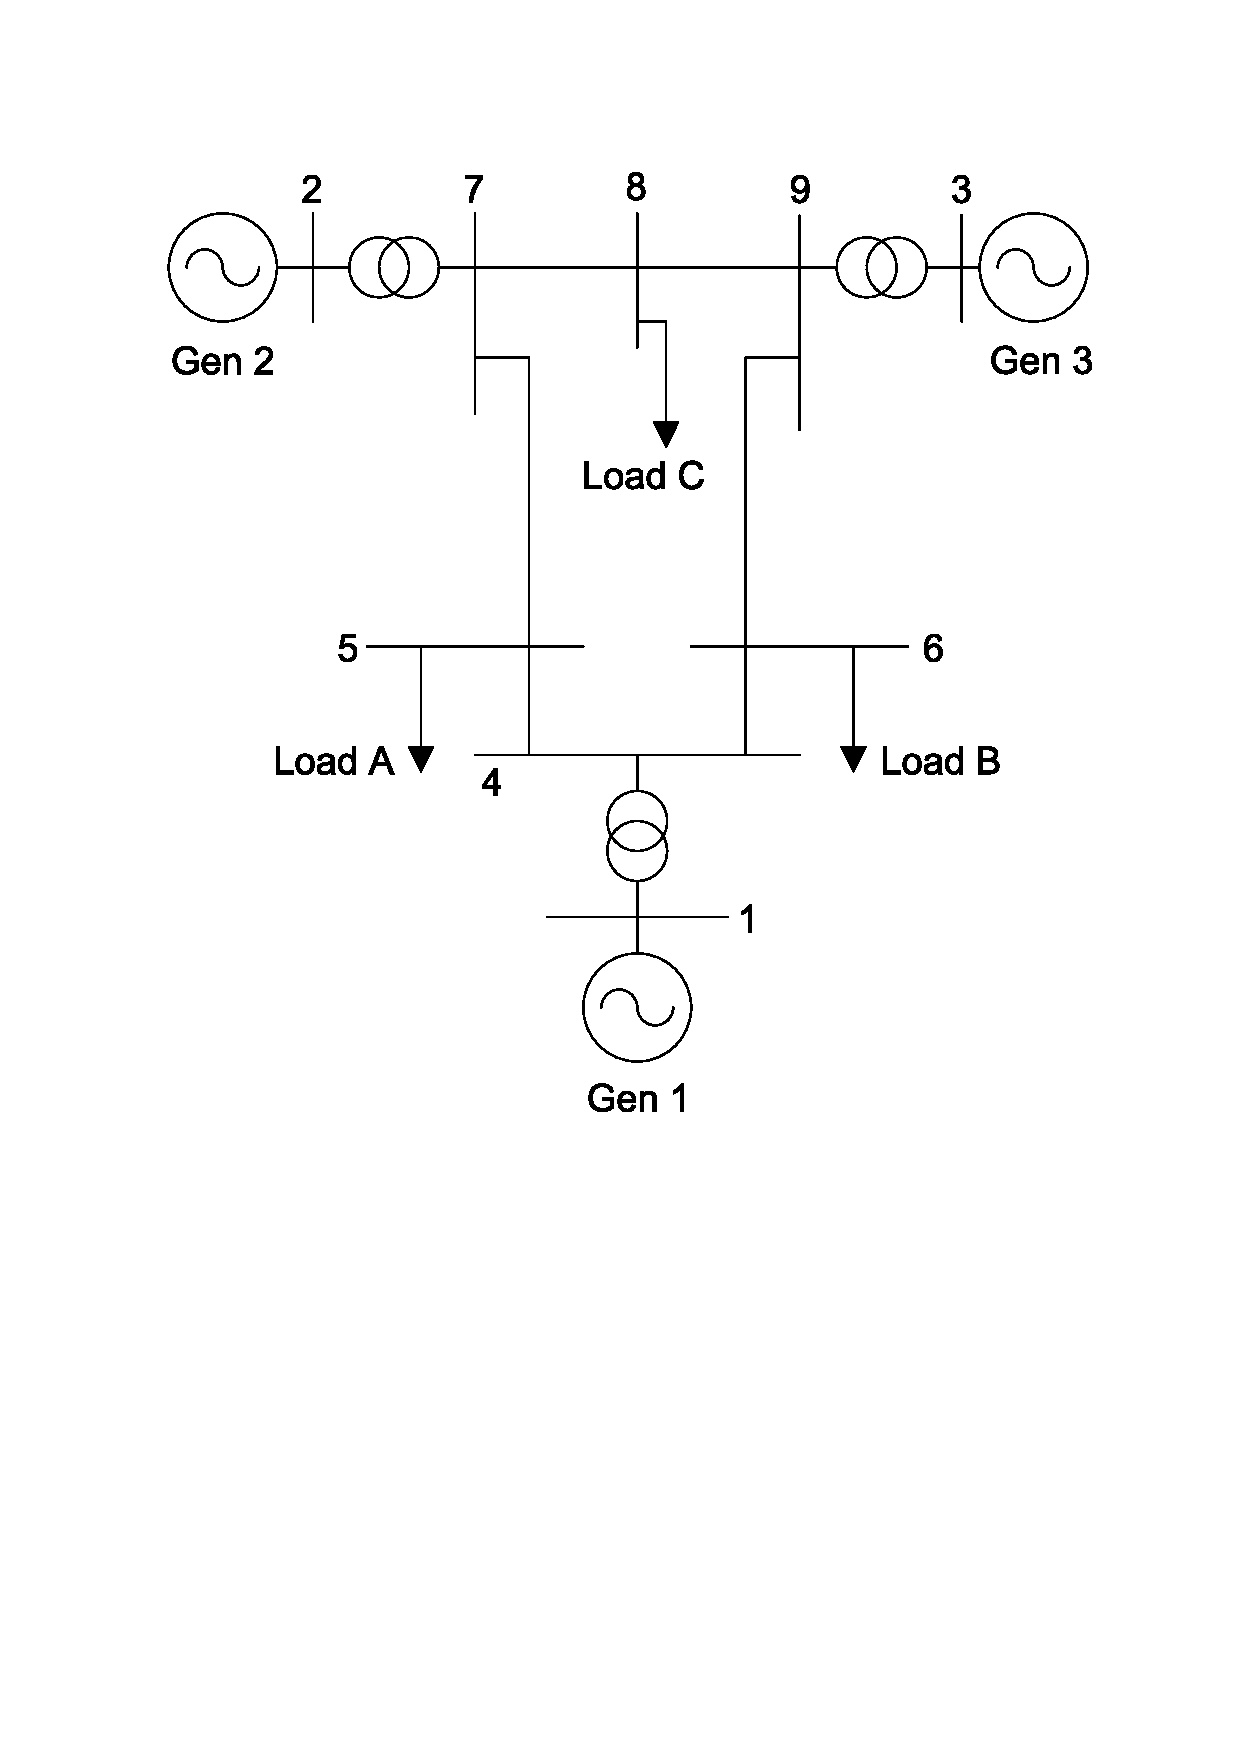
\includegraphics[width=\textwidth]{Figs/Ieee9bus.pdf}
\column{0.5\textwidth}
% This file was created by matlab2tikz v0.4.1.
% Copyright (c) 2008--2013, Nico Schlömer <nico.schloemer@gmail.com>
% All rights reserved.
% 
% The latest updates can be retrieved from
%   http://www.mathworks.com/matlabcentral/fileexchange/22022-matlab2tikz
% where you can also make suggestions and rate matlab2tikz.
% 
% 
% 
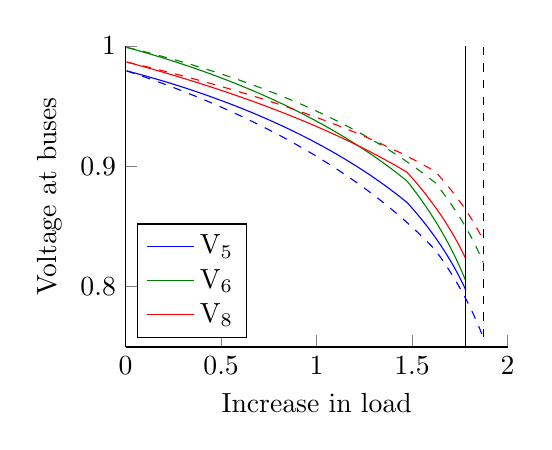
\begin{tikzpicture}

\begin{axis}[%
width=\fwidth,
height=0.788709677419355\fwidth,
scale only axis,
xmin=0,
xmax=2,
xlabel={Increase in load},
ymin=0.75,
ymax=1,
ylabel={Voltage at buses},
axis x line*=bottom,
axis y line*=left,
legend style={draw=black,fill=white,legend cell align=left},
legend pos=south west,
]
\addplot [
color=blue,
solid
]
table[row sep=crcr]{
0.005 0.979232052476942\\
0.01 0.97902472499685\\
0.015 0.978816627748652\\
0.02 0.978607758936801\\
0.025 0.978398116752672\\
0.03 0.978187699374455\\
0.035 0.977976504967064\\
0.04 0.977764531682033\\
0.045 0.977551777657413\\
0.05 0.977338241017672\\
0.055 0.977123919873591\\
0.06 0.976908812322158\\
0.065 0.976692916446462\\
0.07 0.976476230315584\\
0.075 0.976258751984497\\
0.08 0.97604047949394\\
0.085 0.975821410870326\\
0.09 0.975601544125613\\
0.095 0.975380877257204\\
0.1 0.975159408247819\\
0.105 0.974937135065394\\
0.11 0.974714055662948\\
0.115 0.974490167978475\\
0.12 0.97426546993482\\
0.125 0.974039959439555\\
0.13 0.973813634384864\\
0.135 0.97358649264741\\
0.14 0.973358532088208\\
0.145 0.973129750552511\\
0.15 0.972900145869665\\
0.155 0.972669715852988\\
0.16 0.972438458299638\\
0.165 0.972206370990475\\
0.17 0.971973451689931\\
0.175 0.971739698145868\\
0.18 0.971505108089446\\
0.185 0.971269679234981\\
0.19 0.971033409279799\\
0.195 0.9707962959041\\
0.2 0.970558336770811\\
0.205 0.970319529525434\\
0.21 0.970079871795907\\
0.215 0.969839361192448\\
0.22 0.969597995307403\\
0.225 0.969355771715097\\
0.23 0.96911268797167\\
0.235 0.968868741614931\\
0.24 0.96862393016419\\
0.245 0.968378251120101\\
0.25 0.968131701964495\\
0.255 0.967884280160218\\
0.26 0.967635983150967\\
0.265 0.967386808361114\\
0.27 0.967136753195537\\
0.275 0.966885815039451\\
0.28 0.966633991258225\\
0.285 0.966381279197213\\
0.29 0.966127676181567\\
0.295 0.965873179516057\\
0.3 0.965617786484891\\
0.305 0.965361494351521\\
0.31 0.965104300358459\\
0.315 0.964846201727088\\
0.32 0.964587195657461\\
0.325 0.96432727932811\\
0.33 0.964066449895848\\
0.335 0.963804704495564\\
0.34 0.963542040240023\\
0.345 0.96327845421966\\
0.35 0.963013943502367\\
0.355 0.962748505133287\\
0.36 0.962482136134595\\
0.365 0.962214833505284\\
0.37 0.961946594220946\\
0.375 0.961677415233546\\
0.38 0.9614072934712\\
0.385 0.961136225837946\\
0.39 0.96086420921351\\
0.395 0.960591240453077\\
0.4 0.960317316387048\\
0.405 0.960042433820804\\
0.41 0.959766589534459\\
0.415 0.959489780282617\\
0.42 0.959212002794118\\
0.425 0.958933253771787\\
0.43 0.958653529892179\\
0.435 0.958372827805316\\
0.44 0.958091144134421\\
0.445 0.957808475475659\\
0.45 0.95752481839786\\
0.455 0.957240169442246\\
0.46 0.956954525122153\\
0.465 0.956667881922752\\
0.47 0.956380236300759\\
0.475 0.956091584684149\\
0.48 0.955801923471864\\
0.485 0.955511249033509\\
0.49 0.955219557709055\\
0.495 0.954926845808539\\
0.5 0.954633109611744\\
0.505 0.95433834536789\\
0.51 0.954042549295318\\
0.515 0.953745717581161\\
0.52 0.953447846381022\\
0.525 0.953148931818643\\
0.53 0.952848969985562\\
0.535 0.952547956940778\\
0.54 0.952245888710402\\
0.545 0.951942761287309\\
0.55 0.951638570630777\\
0.555 0.951333312666132\\
0.56 0.951026983284377\\
0.565 0.950719578341824\\
0.57 0.950411093659716\\
0.575 0.950101525023845\\
0.58 0.949790868184165\\
0.585 0.949479118854398\\
0.59 0.949166272711636\\
0.595 0.948852325395935\\
0.6 0.948537272509908\\
0.605 0.948221109618302\\
0.61 0.947903832247581\\
0.615 0.947585435885496\\
0.62 0.947265915980647\\
0.625 0.946945267942044\\
0.63 0.946623487138658\\
0.635 0.946300568898964\\
0.64 0.945976508510484\\
0.645 0.945651301219311\\
0.65 0.945324942229641\\
0.655 0.944997426703284\\
0.66 0.944668749759176\\
0.665 0.944338906472882\\
0.67 0.944007891876088\\
0.675 0.943675700956093\\
0.68 0.943342328655279\\
0.685000000000001 0.943007769870591\\
0.690000000000001 0.942672019452993\\
0.695000000000001 0.94233507220693\\
0.700000000000001 0.941996922889765\\
0.705000000000001 0.941657566211222\\
0.710000000000001 0.941316996832811\\
0.715000000000001 0.940975209367252\\
0.720000000000001 0.94063219837788\\
0.725000000000001 0.940287958378049\\
0.730000000000001 0.939942483830522\\
0.735000000000001 0.939595769146855\\
0.740000000000001 0.939247808686765\\
0.745000000000001 0.938898596757493\\
0.750000000000001 0.938548127613157\\
0.755000000000001 0.938196395454092\\
0.760000000000001 0.937843394426179\\
0.765000000000001 0.937489118620167\\
0.770000000000001 0.937133562070975\\
0.775000000000001 0.936776718756997\\
0.780000000000001 0.93641858259938\\
0.785000000000001 0.936059147461303\\
0.790000000000001 0.935698407147235\\
0.795000000000001 0.935336355402183\\
0.800000000000001 0.934972985910932\\
0.805000000000001 0.934608292297266\\
0.810000000000001 0.93424226812318\\
0.815000000000001 0.933874906888075\\
0.820000000000001 0.933506202027946\\
0.825000000000001 0.933136146914546\\
0.830000000000001 0.932764734854547\\
0.835000000000001 0.932391959088675\\
0.840000000000001 0.932017812790845\\
0.845000000000001 0.931642289067262\\
0.850000000000001 0.931265380955526\\
0.855000000000001 0.930887081423705\\
0.860000000000001 0.930507383369403\\
0.865000000000001 0.930126279618808\\
0.870000000000001 0.929743762925718\\
0.875000000000001 0.929359825970559\\
0.880000000000001 0.928974461359383\\
0.885000000000001 0.928587661622839\\
0.890000000000001 0.928199419215138\\
0.895000000000001 0.927809726512996\\
0.900000000000001 0.927418575814553\\
0.905000000000001 0.927025959338274\\
0.910000000000001 0.926631869221839\\
0.915000000000001 0.926236297520995\\
0.920000000000001 0.925839236208407\\
0.925000000000001 0.925440677172475\\
0.930000000000001 0.925040612216129\\
0.935000000000001 0.924639033055613\\
0.940000000000001 0.924235931319227\\
0.945000000000001 0.923831298546071\\
0.950000000000001 0.923425126184737\\
0.955000000000001 0.923017405592005\\
0.960000000000001 0.922608128031487\\
0.965000000000001 0.922197284672269\\
0.970000000000001 0.921784866587509\\
0.975000000000001 0.921370864753017\\
0.980000000000001 0.920955270045811\\
0.985000000000001 0.920538073242635\\
0.990000000000001 0.920119265018455\\
0.995000000000001 0.919698835944925\\
1 0.919276776488821\\
1.005 0.918853077010446\\
1.01 0.918427727762004\\
1.015 0.91800071888594\\
1.02 0.917572040413243\\
1.025 0.917141682261728\\
1.03 0.916709634234268\\
1.035 0.916275886017003\\
1.04 0.9158404271775\\
1.045 0.915403247162889\\
1.05 0.914964335297953\\
1.055 0.914523680783177\\
1.06 0.914081272692762\\
1.065 0.913637099972596\\
1.07 0.913191151438185\\
1.075 0.912743415772529\\
1.08 0.912293881523976\\
1.085 0.911842537104001\\
1.09 0.911389370784969\\
1.095 0.910934370697825\\
1.1 0.91047752482975\\
1.105 0.910018821021757\\
1.11 0.909558246966245\\
1.115 0.909095790204486\\
1.12 0.908631438124073\\
1.125 0.908165177956298\\
1.13 0.907696996773481\\
1.135 0.907226881486238\\
1.14 0.906754818840685\\
1.145 0.906280795415581\\
1.15 0.90580479761941\\
1.155 0.905326811687392\\
1.16 0.904846823678429\\
1.165 0.90436481947198\\
1.17 0.903880784764868\\
1.175 0.903394705068004\\
1.18 0.902906565703046\\
1.185 0.902416351798974\\
1.19 0.901924048288587\\
1.195 0.901429639904913\\
1.2 0.900933111177543\\
1.20497298395187 0.900437146584785\\
1.20992526856465 0.899941131037016\\
1.21485696063708 0.899445064689713\\
1.21976816591341 0.898948947696048\\
1.22465898907991 0.898452780206842\\
1.22952953378013 0.897956562370589\\
1.23437990262991 0.897460294333487\\
1.23921019723211 0.896963976239474\\
1.2440205181911 0.896467608230245\\
1.24881096512691 0.895971190445292\\
1.25358163668918 0.895474723021924\\
1.25833263057079 0.894978206095298\\
1.26306404352137 0.894481639798445\\
1.26777597136041 0.893985024262295\\
1.27246850899021 0.893488359615704\\
1.27714175040859 0.89299164598548\\
1.28179578872141 0.892494883496404\\
1.28643071615476 0.89199807227126\\
1.29104662406705 0.891501212430853\\
1.29564360296083 0.891004304094036\\
1.30022174249439 0.890507347377731\\
1.30478113149316 0.890010342396953\\
1.30932185796096 0.889513289264831\\
1.31384400909099 0.88901618809263\\
1.31834767127666 0.888519038989772\\
1.32283293012223 0.888021842063856\\
1.32729987045327 0.887524597420682\\
1.33174857632692 0.887027305164266\\
1.336179131042 0.886529965396862\\
1.34059161714895 0.886032578218982\\
1.34498611645954 0.885535143729415\\
1.34936271005653 0.885037662025244\\
1.35372147830306 0.884540133201866\\
1.35806250085191 0.884042557353006\\
1.36238585665466 0.883544934570742\\
1.36669162397063 0.883047264945515\\
1.37097988037572 0.88254954856615\\
1.37525070277103 0.882051785519872\\
1.37950416739145 0.881553975892319\\
1.38374034981404 0.881056119767564\\
1.38795932496622 0.880558217228126\\
1.39216116713397 0.880060268354987\\
1.39634594996977 0.879562273227608\\
1.40051374650046 0.879064231923942\\
1.40466462913498 0.87856614452045\\
1.40879866967199 0.878068011092116\\
1.41291593930731 0.877569831712458\\
1.41701650864131 0.877071606453547\\
1.4211004476862 0.876573335386014\\
1.4251678258731 0.876075018579069\\
1.42921871205906 0.875576656100512\\
1.43325317453404 0.875078248016746\\
1.43727128102765 0.874579794392787\\
1.44127309871588 0.874081295292283\\
1.44525869422766 0.873582750777517\\
1.44922813365137 0.873084160909429\\
1.45318148254125 0.87258552574762\\
1.45711880592367 0.872086845350366\\
1.4610401683033 0.87158811977463\\
1.46494563366927 0.871089349076074\\
1.46883526550114 0.870590533309067\\
1.47270912677483 0.870091672526697\\
1.47579130221616 0.869628004653946\\
1.47829399300274 0.869190161405018\\
1.48078768860855 0.868752308829099\\
1.48327241224409 0.868314447007678\\
1.48574818699804 0.867876576022114\\
1.48821503583894 0.867438695953651\\
1.49067298161619 0.867000806883415\\
1.49312204706092 0.866562908892419\\
1.4955622547869 0.866125002061569\\
1.49799362729146 0.865687086471663\\
1.50041618695643 0.865249162203397\\
1.50282995604894 0.864811229337368\\
1.50523495672237 0.864373287954076\\
1.50763121101719 0.86393533813393\\
1.51001874086183 0.863497379957246\\
1.51239756807352 0.863059413504256\\
1.51476771435915 0.86262143885511\\
1.51712920131609 0.862183456089875\\
1.51948205043304 0.861745465288542\\
1.52182628309083 0.861307466531028\\
1.52416192056321 0.860869459897181\\
1.52648898401772 0.860431445466779\\
1.52880749451639 0.859993423319538\\
1.53111747301665 0.85955539353511\\
1.53341894037198 0.859117356193091\\
1.53571191733276 0.858679311373022\\
1.53799642454702 0.858241259154388\\
1.54027248256119 0.85780319961663\\
1.54254011182085 0.85736513283914\\
1.54479933267149 0.856927058901266\\
1.54705016535919 0.856488977882318\\
1.54929263003143 0.856050889861569\\
1.55152674673775 0.855612794918257\\
1.55375253543047 0.855174693131589\\
1.55597001596542 0.854736584580744\\
1.55817920810264 0.854298469344875\\
1.56038013150704 0.853860347503114\\
1.56257280574913 0.853422219134572\\
1.56475725030568 0.852984084318346\\
1.56693348456037 0.852545943133518\\
1.5691015278045 0.852107795659158\\
1.57126139923764 0.851669641974332\\
1.57341311796827 0.851231482158099\\
1.57555670301444 0.850793316289514\\
1.5776921733044 0.850355144447637\\
1.57981954767726 0.84991696671153\\
1.58193884488359 0.84947878316026\\
1.5840500835861 0.849040593872908\\
1.58615328236017 0.848602398928562\\
1.58824845969456 0.84816419840633\\
1.59033563399195 0.847725992385334\\
1.59241482356956 0.84728778094472\\
1.59448604665977 0.846849564163657\\
1.59654932141069 0.846411342121339\\
1.59860466588672 0.845973114896991\\
1.60065209806919 0.845534882569871\\
1.6026916358569 0.845096645219269\\
1.60472329706666 0.844658402924514\\
1.60674709943393 0.844220155764978\\
1.60876306061331 0.843781903820073\\
1.61077119817912 0.843343647169259\\
1.61277152962596 0.842905385892045\\
1.61476407236924 0.842467120067991\\
1.61674884374571 0.842028849776711\\
1.61872586101402 0.841590575097877\\
1.62069514135523 0.841152296111222\\
1.62265670187335 0.840714012896541\\
1.62461055959583 0.840275725533693\\
1.62655673147413 0.839837434102608\\
1.62849523438416 0.839399138683286\\
1.63042608512686 0.8389608393558\\
1.63234930042862 0.8385225362003\\
1.63426489694185 0.838084229297017\\
1.63617289124547 0.837645918726263\\
1.63807329984532 0.837207604568434\\
1.63996613917473 0.836769286904015\\
1.64185142559497 0.836330965813581\\
1.64372917539571 0.8358926413778\\
1.6455994047955 0.835454313677436\\
1.64746212994226 0.835015982793352\\
1.64931736691372 0.834577648806512\\
1.65116513171786 0.834139311797985\\
1.65300544029344 0.833700971848945\\
1.65483830851035 0.833262629040678\\
1.65666375217014 0.832824283454581\\
1.65848178700643 0.832385935172168\\
1.66029242868532 0.831947584275069\\
1.6620956928059 0.831509230845035\\
1.66389159490061 0.831070874963942\\
1.66568015043572 0.830632516713791\\
1.6674613748117 0.830194156176713\\
1.6692352833637 0.82975579343497\\
1.67100189136193 0.829317428570958\\
1.67276121401209 0.828879061667212\\
1.67451326645577 0.828440692806407\\
1.67625806377087 0.82800232207136\\
1.67799562097198 0.827563949545034\\
1.6797259530108 0.827125575310542\\
1.68144907477654 0.826687199451146\\
1.68316500109629 0.826248822050264\\
1.68487374673544 0.82581044319147\\
1.68657532639803 0.825372062958497\\
1.68826975472718 0.824933681435243\\
1.68995704630543 0.82449529870577\\
1.69163721565512 0.824056914854306\\
1.69331027723879 0.823618529965256\\
1.69497624545954 0.823180144123192\\
1.69663513466137 0.822741757412867\\
1.69828695912959 0.822303369919213\\
1.69993173309116 0.821864981727342\\
1.70156947071501 0.821426592922556\\
1.70320018611249 0.82098820359034\\
1.70482389333761 0.820549813816373\\
1.70644060638749 0.820111423686527\\
1.70805033920263 0.819673033286871\\
1.70965310566729 0.819234642703675\\
1.71124891960986 0.818796252023408\\
1.7128377948031 0.818357861332748\\
1.71441974496461 0.81791947071858\\
1.71599478375704 0.817481080267999\\
1.71756292478849 0.817042690068318\\
1.71912418161284 0.816604300207063\\
1.72067856773003 0.816165910771982\\
1.7222260965864 0.815727521851048\\
1.72376678157505 0.815289133532456\\
1.72530063603609 0.814850745904633\\
1.726827673257 0.814412359056236\\
1.72834790647294 0.81397397307616\\
1.72986134886702 0.813535588053534\\
1.73136801357067 0.813097204077732\\
1.73286791366386 0.812658821238369\\
1.73436106217552 0.812220439625308\\
1.7358474720837 0.811782059328663\\
1.73732715631597 0.8113436804388\\
1.73880012774968 0.810905303046343\\
1.74026639921226 0.810466927242172\\
1.7417259834815 0.810028553117432\\
1.74317889328582 0.809590180763534\\
1.7446251413046 0.809151810272155\\
1.74606474016843 0.808713441735246\\
1.7474977024594 0.808275075245032\\
1.74892404071139 0.807836710894016\\
1.75034376741033 0.807398348774981\\
1.75175689499446 0.806959988980998\\
1.75316343585465 0.80652163160542\\
1.75456340233463 0.806083276741896\\
1.75595680673126 0.805644924484365\\
1.75734366129481 0.805206574927065\\
1.75872397822922 0.804768228164535\\
1.76009776969238 0.804329884291616\\
1.76146504779632 0.803891543403457\\
1.76282582460756 0.803453205595516\\
1.76418011214731 0.803014870963566\\
1.76552792239173 0.802576539603695\\
1.76686926727219 0.802138211612313\\
1.76820415867552 0.801699887086152\\
1.76953260844424 0.801261566122271\\
1.77085462837683 0.80082324881806\\
1.77217023022798 0.800384935271242\\
1.77347942570878 0.799946625579877\\
1.77478222648702 0.799508319842363\\
1.7760786441874 0.799070018157447\\
1.77736869039176 0.798631720624219\\
1.77865237663933 0.798193427342121\\
1.77992971442697 0.797755138410948\\
1.78120071520936 0.797316853930855\\
};
\addlegendentry{$\text{V}_\text{5}$};

\addplot [
color=green!50!black,
solid
]
table[row sep=crcr]{
0.005 0.998686038128165\\
0.01 0.998470807513519\\
0.015 0.998254815896074\\
0.02 0.998038061500132\\
0.025 0.997820542537159\\
0.03 0.997602257205685\\
0.035 0.997383203691213\\
0.04 0.997163380166114\\
0.045 0.996942784789531\\
0.05 0.996721415707276\\
0.055 0.996499271051735\\
0.06 0.996276348941757\\
0.065 0.996052647482554\\
0.07 0.995828164765599\\
0.075 0.995602898868513\\
0.08 0.995376847854963\\
0.085 0.995150009774552\\
0.09 0.994922382662708\\
0.095 0.994693964540574\\
0.1 0.994464753414892\\
0.105 0.9942347472779\\
0.11 0.994003944107203\\
0.115 0.993772341865665\\
0.12 0.993539938501291\\
0.125 0.993306731947106\\
0.13 0.993072720121036\\
0.135 0.992837900925786\\
0.14 0.992602272248714\\
0.145 0.992365831961713\\
0.15 0.992128577921079\\
0.155 0.991890507967386\\
0.16 0.991651619925355\\
0.165 0.99141191160373\\
0.17 0.991171380795137\\
0.175 0.990930025275956\\
0.18 0.990687842806186\\
0.185 0.990444831129306\\
0.19 0.990200987972138\\
0.195 0.989956311044708\\
0.2 0.989710798040102\\
0.205 0.989464446634324\\
0.21 0.989217254486153\\
0.215 0.988969219236992\\
0.22 0.988720338510728\\
0.225 0.988470609913568\\
0.23 0.9882200310339\\
0.235 0.987968599442133\\
0.24 0.987716312690542\\
0.245 0.987463168313114\\
0.25 0.987209163825381\\
0.255 0.986954296724267\\
0.26 0.98669856448792\\
0.265 0.986441964575546\\
0.27 0.986184494427244\\
0.275 0.985926151463838\\
0.28 0.9856669330867\\
0.285 0.985406836677582\\
0.29 0.985145859598439\\
0.295 0.984883999191248\\
0.3 0.984621252777832\\
0.305 0.984357617659675\\
0.31 0.98409309111774\\
0.315 0.983827670412279\\
0.32 0.983561352782646\\
0.325 0.983294135447103\\
0.33 0.983026015602632\\
0.335 0.982756990424732\\
0.34 0.982487057067221\\
0.345 0.982216212662041\\
0.35 0.981944454319044\\
0.355 0.981671779125794\\
0.36 0.981398184147355\\
0.365 0.981123666426076\\
0.37 0.980848222981382\\
0.375 0.980571850809553\\
0.38 0.980294546883505\\
0.385 0.980016308152566\\
0.39 0.979737131542254\\
0.395 0.979457013954042\\
0.4 0.979175952265133\\
0.405 0.97889394332822\\
0.41 0.978610983971251\\
0.415 0.978327070997188\\
0.42 0.978042201183761\\
0.425 0.977756371283223\\
0.43 0.977469578022098\\
0.435 0.97718181810093\\
0.44 0.976893088194018\\
0.445 0.976603384949168\\
0.45 0.976312704987417\\
0.455 0.97602104490277\\
0.46 0.975728401261932\\
0.465 0.975434770604026\\
0.47 0.975140149440322\\
0.475 0.974844534253947\\
0.48 0.974547921499608\\
0.485 0.97425030760329\\
0.49 0.973951688961974\\
0.495 0.973652061943331\\
0.5 0.973351422885422\\
0.505 0.973049768096394\\
0.51 0.972747093854166\\
0.515 0.972443396406114\\
0.52 0.972138671968755\\
0.525 0.971832916727424\\
0.53 0.971526126835937\\
0.535 0.971218298416271\\
0.54 0.970909427558217\\
0.545 0.97059951031904\\
0.55 0.970288542723136\\
0.555 0.969976520761674\\
0.56 0.969663440392244\\
0.565 0.96934929753849\\
0.57 0.96903408808975\\
0.575 0.968717807900674\\
0.58 0.968400452790854\\
0.585 0.968082018544437\\
0.59 0.967762500909739\\
0.595 0.967441895598846\\
0.6 0.967120198287216\\
0.605 0.966797404613275\\
0.61 0.966473510178001\\
0.615 0.966148510544509\\
0.62 0.965822401237626\\
0.625 0.965495177743459\\
0.63 0.965166835508959\\
0.635 0.964837369941478\\
0.64 0.964506776408318\\
0.645 0.964175050236276\\
0.65 0.963842186711176\\
0.655 0.963508181077405\\
0.66 0.963173028537426\\
0.665 0.962836724251306\\
0.67 0.962499263336208\\
0.675 0.962160640865904\\
0.68 0.96182085187026\\
0.685000000000001 0.961479891334724\\
0.690000000000001 0.961137754199798\\
0.695000000000001 0.960794435360515\\
0.700000000000001 0.96044992966589\\
0.705000000000001 0.960104231918377\\
0.710000000000001 0.959757336873312\\
0.715000000000001 0.959409239238344\\
0.720000000000001 0.959059933672865\\
0.725000000000001 0.958709414787425\\
0.730000000000001 0.958357677143137\\
0.735000000000001 0.95800471525108\\
0.740000000000001 0.957650523571678\\
0.745000000000001 0.95729509651409\\
0.750000000000001 0.95693842843557\\
0.755000000000001 0.956580513640829\\
0.760000000000001 0.95622134638138\\
0.765000000000001 0.955860920854878\\
0.770000000000001 0.955499231204446\\
0.775000000000001 0.955136271517989\\
0.780000000000001 0.954772035827498\\
0.785000000000001 0.954406518108345\\
0.790000000000001 0.954039712278562\\
0.795000000000001 0.95367161219811\\
0.800000000000001 0.953302211668138\\
0.805000000000001 0.952931504430224\\
0.810000000000001 0.952559484165609\\
0.815000000000001 0.952186144494416\\
0.820000000000001 0.951811478974857\\
0.825000000000001 0.951435481102418\\
0.830000000000001 0.951058144309046\\
0.835000000000001 0.95067946196231\\
0.840000000000001 0.950299427364549\\
0.845000000000001 0.949918033752009\\
0.850000000000001 0.949535274293966\\
0.855000000000001 0.949151142091824\\
0.860000000000001 0.948765630178213\\
0.865000000000001 0.948378731516058\\
0.870000000000001 0.947990438997632\\
0.875000000000001 0.947600745443607\\
0.880000000000001 0.94720964360207\\
0.885000000000001 0.946817126147532\\
0.890000000000001 0.946423185679912\\
0.895000000000001 0.946027814723517\\
0.900000000000001 0.945631005725988\\
0.905000000000001 0.945232751057228\\
0.910000000000001 0.944833043008327\\
0.915000000000001 0.944431873790448\\
0.920000000000001 0.944029235533704\\
0.925000000000001 0.943625120286008\\
0.930000000000001 0.943219520011909\\
0.935000000000001 0.9428124265914\\
0.940000000000001 0.942403831818708\\
0.945000000000001 0.941993727401055\\
0.950000000000001 0.941582104957407\\
0.955000000000001 0.941168956017191\\
0.960000000000001 0.940754272018985\\
0.965000000000001 0.940338044309195\\
0.970000000000001 0.939920264140697\\
0.975000000000001 0.93950092267145\\
0.980000000000001 0.939080010963102\\
0.985000000000001 0.93865751997954\\
0.990000000000001 0.938233440585439\\
0.995000000000001 0.937807763544761\\
1 0.937380479519245\\
1.005 0.936951579066849\\
1.01 0.936521052640174\\
1.015 0.93608889058485\\
1.02 0.935655083137893\\
1.025 0.935219620426027\\
1.03 0.934782492463977\\
1.035 0.93434368915272\\
1.04 0.933903200277709\\
1.045 0.933461015507054\\
1.05 0.933017124389671\\
1.055 0.932571516353387\\
1.06 0.932124180703016\\
1.065 0.931675106618382\\
1.07 0.931224283152313\\
1.075 0.930771699228586\\
1.08 0.93031734363983\\
1.085 0.929861205045387\\
1.09 0.929403271969127\\
1.095 0.928943532797212\\
1.1 0.928481975775821\\
1.105 0.928018589008819\\
1.11 0.927553360455379\\
1.115 0.927086277927544\\
1.12 0.926617329087758\\
1.125 0.926146501446313\\
1.13 0.925673782358763\\
1.135 0.925199159023272\\
1.14 0.924722618477902\\
1.145 0.924244147597843\\
1.15 0.923763733092579\\
1.155 0.923281361502994\\
1.16 0.922797019198407\\
1.165 0.922310692373541\\
1.17 0.92182236704543\\
1.175 0.921332029050237\\
1.18 0.920839664040022\\
1.185 0.920345257479411\\
1.19 0.919848794642212\\
1.195 0.919350260607925\\
1.2 0.918849640258189\\
1.20497298395187 0.918349640258189\\
1.20992526856465 0.917849640258189\\
1.21485696063708 0.91734964025819\\
1.21976816591341 0.91684964025819\\
1.22465898907991 0.91634964025819\\
1.22952953378013 0.91584964025819\\
1.23437990262991 0.91534964025819\\
1.23921019723211 0.91484964025819\\
1.2440205181911 0.91434964025819\\
1.24881096512691 0.91384964025819\\
1.25358163668918 0.91334964025819\\
1.25833263057079 0.912849640258191\\
1.26306404352137 0.912349640258191\\
1.26777597136041 0.911849640258191\\
1.27246850899021 0.911349640258191\\
1.27714175040859 0.910849640258191\\
1.28179578872141 0.910349640258191\\
1.28643071615476 0.909849640258191\\
1.29104662406705 0.909349640258191\\
1.29564360296083 0.908849640258191\\
1.30022174249439 0.908349640258191\\
1.30478113149316 0.907849640258192\\
1.30932185796096 0.907349640258192\\
1.31384400909099 0.906849640258192\\
1.31834767127666 0.906349640258192\\
1.32283293012223 0.905849640258192\\
1.32729987045327 0.905349640258192\\
1.33174857632692 0.904849640258192\\
1.336179131042 0.904349640258192\\
1.34059161714895 0.903849640258192\\
1.34498611645954 0.903349640258192\\
1.34936271005653 0.902849640258192\\
1.35372147830306 0.902349640258192\\
1.35806250085191 0.901849640258192\\
1.36238585665466 0.901349640258192\\
1.36669162397063 0.900849640258192\\
1.37097988037572 0.900349640258192\\
1.37525070277103 0.899849640258192\\
1.37950416739145 0.899349640258192\\
1.38374034981404 0.898849640258192\\
1.38795932496622 0.898349640258192\\
1.39216116713397 0.897849640258192\\
1.39634594996977 0.897349640258193\\
1.40051374650046 0.896849640258193\\
1.40466462913498 0.896349640258193\\
1.40879866967199 0.895849640258193\\
1.41291593930731 0.895349640258193\\
1.41701650864131 0.894849640258193\\
1.4211004476862 0.894349640258193\\
1.4251678258731 0.893849640258193\\
1.42921871205906 0.893349640258193\\
1.43325317453404 0.892849640258193\\
1.43727128102765 0.892349640258193\\
1.44127309871588 0.891849640258193\\
1.44525869422766 0.891349640258193\\
1.44922813365137 0.890849640258193\\
1.45318148254125 0.890349640258193\\
1.45711880592367 0.889849640258193\\
1.4610401683033 0.889349640258193\\
1.46494563366927 0.888849640258193\\
1.46883526550114 0.888349640258193\\
1.47270912677483 0.887849640258193\\
1.47579130221616 0.887349640258193\\
1.47829399300274 0.886849640258193\\
1.48078768860855 0.886349640258193\\
1.48327241224409 0.885849640258193\\
1.48574818699804 0.885349640258193\\
1.48821503583894 0.884849640258193\\
1.49067298161619 0.884349640258194\\
1.49312204706092 0.883849640258194\\
1.4955622547869 0.883349640258194\\
1.49799362729146 0.882849640258194\\
1.50041618695643 0.882349640258194\\
1.50282995604894 0.881849640258194\\
1.50523495672237 0.881349640258194\\
1.50763121101719 0.880849640258194\\
1.51001874086183 0.880349640258194\\
1.51239756807352 0.879849640258194\\
1.51476771435915 0.879349640258194\\
1.51712920131609 0.878849640258194\\
1.51948205043304 0.878349640258194\\
1.52182628309083 0.877849640258194\\
1.52416192056321 0.877349640258195\\
1.52648898401772 0.876849640258195\\
1.52880749451639 0.876349640258195\\
1.53111747301665 0.875849640258195\\
1.53341894037198 0.875349640258195\\
1.53571191733276 0.874849640258195\\
1.53799642454702 0.874349640258195\\
1.54027248256119 0.873849640258195\\
1.54254011182085 0.873349640258195\\
1.54479933267149 0.872849640258195\\
1.54705016535919 0.872349640258195\\
1.54929263003143 0.871849640258195\\
1.55152674673775 0.871349640258196\\
1.55375253543047 0.870849640258195\\
1.55597001596542 0.870349640258196\\
1.55817920810264 0.869849640258196\\
1.56038013150704 0.869349640258196\\
1.56257280574913 0.868849640258196\\
1.56475725030568 0.868349640258196\\
1.56693348456037 0.867849640258196\\
1.5691015278045 0.867349640258196\\
1.57126139923764 0.866849640258196\\
1.57341311796827 0.866349640258196\\
1.57555670301444 0.865849640258196\\
1.5776921733044 0.865349640258196\\
1.57981954767726 0.864849640258196\\
1.58193884488359 0.864349640258196\\
1.5840500835861 0.863849640258196\\
1.58615328236017 0.863349640258196\\
1.58824845969456 0.862849640258197\\
1.59033563399195 0.862349640258197\\
1.59241482356956 0.861849640258197\\
1.59448604665977 0.861349640258197\\
1.59654932141069 0.860849640258197\\
1.59860466588672 0.860349640258197\\
1.60065209806919 0.859849640258197\\
1.6026916358569 0.859349640258197\\
1.60472329706666 0.858849640258197\\
1.60674709943393 0.858349640258197\\
1.60876306061331 0.857849640258197\\
1.61077119817912 0.857349640258197\\
1.61277152962596 0.856849640258197\\
1.61476407236924 0.856349640258197\\
1.61674884374571 0.855849640258197\\
1.61872586101402 0.855349640258197\\
1.62069514135523 0.854849640258197\\
1.62265670187335 0.854349640258197\\
1.62461055959583 0.853849640258198\\
1.62655673147413 0.853349640258198\\
1.62849523438416 0.852849640258198\\
1.63042608512686 0.852349640258198\\
1.63234930042862 0.851849640258198\\
1.63426489694185 0.851349640258198\\
1.63617289124547 0.850849640258198\\
1.63807329984532 0.850349640258198\\
1.63996613917473 0.849849640258198\\
1.64185142559497 0.849349640258198\\
1.64372917539571 0.848849640258198\\
1.6455994047955 0.848349640258198\\
1.64746212994226 0.847849640258198\\
1.64931736691372 0.847349640258198\\
1.65116513171786 0.846849640258198\\
1.65300544029344 0.846349640258198\\
1.65483830851035 0.845849640258198\\
1.65666375217014 0.845349640258198\\
1.65848178700643 0.844849640258199\\
1.66029242868532 0.844349640258199\\
1.6620956928059 0.843849640258199\\
1.66389159490061 0.843349640258199\\
1.66568015043572 0.842849640258199\\
1.6674613748117 0.842349640258199\\
1.6692352833637 0.841849640258199\\
1.67100189136193 0.841349640258199\\
1.67276121401209 0.840849640258199\\
1.67451326645577 0.840349640258199\\
1.67625806377087 0.8398496402582\\
1.67799562097198 0.8393496402582\\
1.6797259530108 0.8388496402582\\
1.68144907477654 0.8383496402582\\
1.68316500109629 0.8378496402582\\
1.68487374673544 0.8373496402582\\
1.68657532639803 0.8368496402582\\
1.68826975472718 0.8363496402582\\
1.68995704630543 0.8358496402582\\
1.69163721565512 0.8353496402582\\
1.69331027723879 0.8348496402582\\
1.69497624545954 0.8343496402582\\
1.69663513466137 0.8338496402582\\
1.69828695912959 0.8333496402582\\
1.69993173309116 0.8328496402582\\
1.70156947071501 0.8323496402582\\
1.70320018611249 0.8318496402582\\
1.70482389333761 0.8313496402582\\
1.70644060638749 0.8308496402582\\
1.70805033920263 0.8303496402582\\
1.70965310566729 0.8298496402582\\
1.71124891960986 0.8293496402582\\
1.7128377948031 0.828849640258201\\
1.71441974496461 0.828349640258201\\
1.71599478375704 0.827849640258201\\
1.71756292478849 0.827349640258201\\
1.71912418161284 0.826849640258201\\
1.72067856773003 0.826349640258201\\
1.7222260965864 0.825849640258201\\
1.72376678157505 0.825349640258201\\
1.72530063603609 0.824849640258201\\
1.726827673257 0.824349640258201\\
1.72834790647294 0.823849640258201\\
1.72986134886702 0.823349640258201\\
1.73136801357067 0.822849640258201\\
1.73286791366386 0.822349640258201\\
1.73436106217552 0.821849640258201\\
1.7358474720837 0.821349640258201\\
1.73732715631597 0.820849640258201\\
1.73880012774968 0.820349640258201\\
1.74026639921226 0.819849640258201\\
1.7417259834815 0.819349640258201\\
1.74317889328582 0.818849640258202\\
1.7446251413046 0.818349640258202\\
1.74606474016843 0.817849640258202\\
1.7474977024594 0.817349640258202\\
1.74892404071139 0.816849640258202\\
1.75034376741033 0.816349640258202\\
1.75175689499446 0.815849640258202\\
1.75316343585465 0.815349640258202\\
1.75456340233463 0.814849640258202\\
1.75595680673126 0.814349640258202\\
1.75734366129481 0.813849640258202\\
1.75872397822922 0.813349640258202\\
1.76009776969238 0.812849640258202\\
1.76146504779632 0.812349640258202\\
1.76282582460756 0.811849640258202\\
1.76418011214731 0.811349640258202\\
1.76552792239173 0.810849640258202\\
1.76686926727219 0.810349640258202\\
1.76820415867552 0.809849640258202\\
1.76953260844424 0.809349640258202\\
1.77085462837683 0.808849640258203\\
1.77217023022798 0.808349640258203\\
1.77347942570878 0.807849640258203\\
1.77478222648702 0.807349640258203\\
1.7760786441874 0.806849640258203\\
1.77736869039176 0.806349640258203\\
1.77865237663933 0.805849640258203\\
1.77992971442697 0.805349640258203\\
1.78120071520936 0.804849640258203\\
};
\addlegendentry{$\text{V}_\text{6}$};

\addplot [
color=red,
solid
]
table[row sep=crcr]{
0.005 0.986518903809878\\
0.01 0.986306414354071\\
0.015 0.986093465368436\\
0.02 0.985880055702197\\
0.025 0.985666184196952\\
0.03 0.985451849686603\\
0.035 0.985237050997311\\
0.04 0.985021786947427\\
0.045 0.984806056347438\\
0.05 0.984589857999902\\
0.055 0.984373190699396\\
0.06 0.984156053232445\\
0.065 0.983938444377469\\
0.07 0.983720362904712\\
0.075 0.983501807576185\\
0.08 0.983282777145597\\
0.085 0.983063270358294\\
0.09 0.982843285951195\\
0.095 0.982622822652718\\
0.1 0.982401879182721\\
0.105 0.982180454252433\\
0.11 0.98195854656438\\
0.115 0.981736154812322\\
0.12 0.981513277681182\\
0.125 0.98128991384697\\
0.13 0.98106606197672\\
0.135 0.980841720728411\\
0.14 0.980616888750893\\
0.145 0.980391564683822\\
0.15 0.980165747157573\\
0.155 0.979939434793175\\
0.16 0.979712626202224\\
0.165 0.979485319986816\\
0.17 0.979257514739463\\
0.175 0.979029209043012\\
0.18 0.978800401470568\\
0.185 0.978571090585416\\
0.19 0.97834127494093\\
0.195 0.978110953080498\\
0.2 0.977880123537435\\
0.205 0.977648784834898\\
0.21 0.9774169354858\\
0.215 0.977184573992724\\
0.22 0.976951698847835\\
0.225 0.976718308532789\\
0.23 0.976484401518647\\
0.235 0.97624997626578\\
0.24 0.976015031223777\\
0.245 0.975779564831356\\
0.25 0.975543575516264\\
0.255 0.975307061695187\\
0.26 0.975070021773648\\
0.265 0.974832454145913\\
0.27 0.974594357194891\\
0.275 0.974355729292033\\
0.28 0.974116568797232\\
0.285 0.97387687405872\\
0.29 0.973636643412963\\
0.295 0.973395875184558\\
0.3 0.973154567686125\\
0.305 0.9729127192182\\
0.31 0.972670328069125\\
0.315 0.972427392514941\\
0.32 0.972183910819273\\
0.325 0.971939881233215\\
0.33 0.971695301995223\\
0.335 0.971450171330992\\
0.34 0.971204487453341\\
0.345 0.970958248562098\\
0.35 0.970711452843971\\
0.355 0.970464098472436\\
0.36 0.970216183607609\\
0.365 0.969967706396118\\
0.37 0.969718664970984\\
0.375 0.969469057451487\\
0.38 0.969218881943041\\
0.385 0.968968136537058\\
0.39 0.968716819310817\\
0.395 0.968464928327333\\
0.4 0.968212461635213\\
0.405 0.967959417268525\\
0.41 0.967705793246657\\
0.415 0.96745158757417\\
0.42 0.96719679824066\\
0.425 0.966941423220611\\
0.43 0.966685460473246\\
0.435 0.966428907942383\\
0.44 0.966171763556277\\
0.445 0.965914025227469\\
0.45 0.965655690852637\\
0.455 0.965396758312426\\
0.46 0.965137225471305\\
0.465 0.964877090177389\\
0.47 0.964616350262289\\
0.475 0.964355003540938\\
0.48 0.964093047811426\\
0.485 0.96383048085483\\
0.49 0.96356730043504\\
0.495 0.963303504298586\\
0.5 0.96303909017446\\
0.505 0.962774055773935\\
0.51 0.962508398790386\\
0.515 0.962242116899102\\
0.52 0.961975207757101\\
0.525 0.96170766900294\\
0.53 0.961439498256522\\
0.535 0.961170693118903\\
0.54 0.960901251172091\\
0.545 0.960631169978851\\
0.55 0.960360447082493\\
0.555 0.960089080006677\\
0.56 0.959817066255194\\
0.565 0.959544403311761\\
0.57 0.959271088639803\\
0.575 0.958997119682236\\
0.58 0.958722493861245\\
0.585 0.958447208578062\\
0.59 0.958171261212734\\
0.595 0.957894649123901\\
0.6 0.95761736964855\\
0.605 0.95733942010179\\
0.61 0.957060797776601\\
0.615 0.956781499943598\\
0.62 0.956501523850775\\
0.625 0.956220866723261\\
0.63 0.955939525763062\\
0.635 0.955657498148799\\
0.64 0.955374781035451\\
0.645 0.955091371554084\\
0.65 0.954807266811581\\
0.655 0.954522463890369\\
0.66 0.95423695984814\\
0.665 0.953950751717566\\
0.67 0.953663836506013\\
0.675 0.953376211195253\\
0.68 0.953087872741161\\
0.685000000000001 0.952798818073419\\
0.690000000000001 0.952509044095212\\
0.695000000000001 0.952218547682914\\
0.700000000000001 0.951927325685779\\
0.705000000000001 0.951635374925616\\
0.710000000000001 0.951342692196468\\
0.715000000000001 0.951049274264282\\
0.720000000000001 0.950755117866576\\
0.725000000000001 0.950460219712096\\
0.730000000000001 0.950164576480474\\
0.735000000000001 0.949868184821875\\
0.740000000000001 0.949571041356644\\
0.745000000000001 0.949273142674942\\
0.750000000000001 0.94897448533638\\
0.755000000000001 0.948675065869643\\
0.760000000000001 0.948374880772116\\
0.765000000000001 0.948073926509492\\
0.770000000000001 0.947772199515387\\
0.775000000000001 0.947469696190939\\
0.780000000000001 0.947166412904399\\
0.785000000000001 0.946862345990731\\
0.790000000000001 0.946557491751183\\
0.795000000000001 0.946251846452869\\
0.800000000000001 0.945945406328337\\
0.805000000000001 0.945638167575126\\
0.810000000000001 0.945330126355326\\
0.815000000000001 0.945021278795119\\
0.820000000000001 0.944711620984321\\
0.825000000000001 0.944401148975914\\
0.830000000000001 0.944089858785565\\
0.835000000000001 0.943777746391144\\
0.840000000000001 0.943464807732235\\
0.845000000000001 0.943151038709626\\
0.850000000000001 0.942836435184805\\
0.855000000000001 0.942520992979438\\
0.860000000000001 0.942204707874844\\
0.865000000000001 0.941887575611457\\
0.870000000000001 0.941569591888278\\
0.875000000000001 0.941250752362321\\
0.880000000000001 0.940931052648048\\
0.885000000000001 0.940610488316789\\
0.890000000000001 0.940289054896163\\
0.895000000000001 0.939966747869478\\
0.900000000000001 0.939643562675123\\
0.905000000000001 0.939319494705954\\
0.910000000000001 0.938994539308662\\
0.915000000000001 0.938668691783134\\
0.920000000000001 0.938341947381803\\
0.925000000000001 0.938014301308985\\
0.930000000000001 0.937685748720196\\
0.935000000000001 0.937356284721477\\
0.940000000000001 0.937025904368681\\
0.945000000000001 0.936694602666765\\
0.950000000000001 0.936362374569065\\
0.955000000000001 0.936029214976551\\
0.960000000000001 0.935695118737077\\
0.965000000000001 0.93536008064461\\
0.970000000000001 0.935024095438446\\
0.975000000000001 0.934687157802417\\
0.980000000000001 0.934349262364072\\
0.985000000000001 0.934010403693855\\
0.990000000000001 0.933670576304254\\
0.995000000000001 0.933329774648945\\
1 0.932987993121914\\
1.005 0.932645226056561\\
1.01 0.932301467724788\\
1.015 0.931956712336072\\
1.02 0.931610954036512\\
1.025 0.931264186907869\\
1.03 0.930916404966574\\
1.035 0.930567602162724\\
1.04 0.930217772379057\\
1.045 0.929866909429903\\
1.05 0.929515007060121\\
1.055 0.929162058944003\\
1.06 0.928808058684166\\
1.065 0.928452999810416\\
1.07 0.928096875778594\\
1.075 0.927739679969385\\
1.08 0.927381405687122\\
1.085 0.927022046158545\\
1.09 0.926661594531548\\
1.095 0.926300043873895\\
1.1 0.925937387171903\\
1.105 0.925573617329111\\
1.11 0.925208727164906\\
1.115 0.924842709413122\\
1.12 0.924475556720623\\
1.125 0.92410726164583\\
1.13 0.923737816657245\\
1.135 0.923367214131913\\
1.14 0.922995446353874\\
1.145 0.922622505512571\\
1.15 0.922248383701218\\
1.155 0.921873072915138\\
1.16 0.921496565050065\\
1.165 0.921118851900401\\
1.17 0.920739925157439\\
1.175 0.92035977640754\\
1.18 0.919978397130277\\
1.185 0.919595778696522\\
1.19 0.919211912366508\\
1.195 0.918826789287825\\
1.2 0.918440400493383\\
1.20497298395187 0.918054834967705\\
1.20992526856465 0.917669612121599\\
1.21485696063708 0.917284730398044\\
1.21976816591341 0.916900188257588\\
1.22465898907991 0.916515984178527\\
1.22952953378013 0.916132116656646\\
1.23437990262991 0.915748584204969\\
1.23921019723211 0.915365385353506\\
1.2440205181911 0.914982518649014\\
1.24881096512691 0.914599982654752\\
1.25358163668918 0.914217775950249\\
1.25833263057079 0.913835897131071\\
1.26306404352137 0.913454344808601\\
1.26777597136041 0.913073117609805\\
1.27246850899021 0.912692214177025\\
1.27714175040859 0.91231163316776\\
1.28179578872141 0.911931373254453\\
1.28643071615476 0.911551433124289\\
1.29104662406705 0.911171811478991\\
1.29564360296083 0.910792507034617\\
1.30022174249439 0.91041351852137\\
1.30478113149316 0.910034844683401\\
1.30932185796096 0.909656484278624\\
1.31384400909099 0.909278436078525\\
1.31834767127666 0.908900698867988\\
1.32283293012223 0.908523271445107\\
1.32729987045327 0.908146152621018\\
1.33174857632692 0.90776934121972\\
1.336179131042 0.907392836077909\\
1.34059161714895 0.907016636044806\\
1.34498611645954 0.906640739982002\\
1.34936271005653 0.906265146763287\\
1.35372147830306 0.905889855274497\\
1.35806250085191 0.905514864413357\\
1.36238585665466 0.905140173089325\\
1.36669162397063 0.904765780223449\\
1.37097988037572 0.904391684748207\\
1.37525070277103 0.904017885607374\\
1.37950416739145 0.90364438175587\\
1.38374034981404 0.903271172159621\\
1.38795932496622 0.902898255795423\\
1.39216116713397 0.902525631650804\\
1.39634594996977 0.902153298723891\\
1.40051374650046 0.901781256023274\\
1.40466462913498 0.901409502567884\\
1.40879866967199 0.901038037386859\\
1.41291593930731 0.900666859519419\\
1.41701650864131 0.900295968014747\\
1.4211004476862 0.899925361931863\\
1.4251678258731 0.899555040339507\\
1.42921871205906 0.899185002316018\\
1.43325317453404 0.898815246949224\\
1.43727128102765 0.898445773336321\\
1.44127309871588 0.898076580583768\\
1.44525869422766 0.897707667807172\\
1.44922813365137 0.897339034131178\\
1.45318148254125 0.896970678689366\\
1.45711880592367 0.896602600624145\\
1.4610401683033 0.896234799086648\\
1.46494563366927 0.895867273236629\\
1.46883526550114 0.895500022242365\\
1.47270912677483 0.895133045280555\\
1.47579130221616 0.894724008875145\\
1.47829399300274 0.8942840627754\\
1.48078768860855 0.893844214065607\\
1.48327241224409 0.89340446234358\\
1.48574818699804 0.892964807208969\\
1.48821503583894 0.892525248263233\\
1.49067298161619 0.892085785109615\\
1.49312204706092 0.89164641735313\\
1.4955622547869 0.891207144600543\\
1.49799362729146 0.890767966460355\\
1.50041618695643 0.890328882542788\\
1.50282995604894 0.889889892459762\\
1.50523495672237 0.889450995824885\\
1.50763121101719 0.889012192253433\\
1.51001874086183 0.888573481362333\\
1.51239756807352 0.888134862770149\\
1.51476771435915 0.887696336097068\\
1.51712920131609 0.887257900964876\\
1.51948205043304 0.886819556996951\\
1.52182628309083 0.886381303818244\\
1.52416192056321 0.885943141055264\\
1.52648898401772 0.885505068336059\\
1.52880749451639 0.885067085290207\\
1.53111747301665 0.884629191548797\\
1.53341894037198 0.884191386744414\\
1.53571191733276 0.883753670511128\\
1.53799642454702 0.883316042484474\\
1.54027248256119 0.882878502301439\\
1.54254011182085 0.882441049600452\\
1.54479933267149 0.882003684021362\\
1.54705016535919 0.881566405205432\\
1.54929263003143 0.881129212795317\\
1.55152674673775 0.880692106435057\\
1.55375253543047 0.880255085770058\\
1.55597001596542 0.879818150447081\\
1.55817920810264 0.879381300114226\\
1.56038013150704 0.878944534420924\\
1.56257280574913 0.878507853017916\\
1.56475725030568 0.878071255557243\\
1.56693348456037 0.877634741692237\\
1.5691015278045 0.8771983110775\\
1.57126139923764 0.876761963368897\\
1.57341311796827 0.87632569822354\\
1.57555670301444 0.875889515299776\\
1.5776921733044 0.875453414257178\\
1.57981954767726 0.875017394756524\\
1.58193884488359 0.874581456459792\\
1.5840500835861 0.874145599030146\\
1.58615328236017 0.87370982213192\\
1.58824845969456 0.873274125430611\\
1.59033563399195 0.872838508592861\\
1.59241482356956 0.872402971286452\\
1.59448604665977 0.871967513180288\\
1.59654932141069 0.871532133944386\\
1.59860466588672 0.871096833249864\\
1.60065209806919 0.870661610768926\\
1.6026916358569 0.870226466174858\\
1.60472329706666 0.869791399142006\\
1.60674709943393 0.869356409345777\\
1.60876306061331 0.868921496462613\\
1.61077119817912 0.868486660169994\\
1.61277152962596 0.868051900146417\\
1.61476407236924 0.867617216071388\\
1.61674884374571 0.867182607625412\\
1.61872586101402 0.86674807448998\\
1.62069514135523 0.866313616347561\\
1.62265670187335 0.865879232881587\\
1.62461055959583 0.865444923776444\\
1.62655673147413 0.865010688717464\\
1.62849523438416 0.86457652739091\\
1.63042608512686 0.864142439483969\\
1.63234930042862 0.863708424684738\\
1.63426489694185 0.863274482682216\\
1.63617289124547 0.862840613166294\\
1.63807329984532 0.862406815827744\\
1.63996613917473 0.861973090358205\\
1.64185142559497 0.861539436450182\\
1.64372917539571 0.861105853797024\\
1.6455994047955 0.860672342092924\\
1.64746212994226 0.860238901032904\\
1.64931736691372 0.859805530312806\\
1.65116513171786 0.859372229629281\\
1.65300544029344 0.858938998679783\\
1.65483830851035 0.858505837162553\\
1.65666375217014 0.858072744776617\\
1.65848178700643 0.857639721221767\\
1.66029242868532 0.857206766198562\\
1.6620956928059 0.856773879408308\\
1.66389159490061 0.856341060553057\\
1.66568015043572 0.855908309335591\\
1.6674613748117 0.855475625459419\\
1.6692352833637 0.855043008628761\\
1.67100189136193 0.854610458548543\\
1.67276121401209 0.854177974924387\\
1.67451326645577 0.853745557462601\\
1.67625806377087 0.853313205870169\\
1.67799562097198 0.852880919854746\\
1.6797259530108 0.852448699124642\\
1.68144907477654 0.852016543388821\\
1.68316500109629 0.851584452356884\\
1.68487374673544 0.851152425739067\\
1.68657532639803 0.850720463246228\\
1.68826975472718 0.850288564589839\\
1.68995704630543 0.849856729481977\\
1.69163721565512 0.849424957635316\\
1.69331027723879 0.848993248763118\\
1.69497624545954 0.848561602579225\\
1.69663513466137 0.848130018798048\\
1.69828695912959 0.847698497134558\\
1.69993173309116 0.847267037304284\\
1.70156947071501 0.846835639023296\\
1.70320018611249 0.846404302008201\\
1.70482389333761 0.845973025976134\\
1.70644060638749 0.845541810644749\\
1.70805033920263 0.845110655732211\\
1.70965310566729 0.844679560957185\\
1.71124891960986 0.844248526038834\\
1.7128377948031 0.843817550696804\\
1.71441974496461 0.843386634651218\\
1.71599478375704 0.84295577762267\\
1.71756292478849 0.842524979332213\\
1.71912418161284 0.842094239501355\\
1.72067856773003 0.841663557852045\\
1.7222260965864 0.841232934106671\\
1.72376678157505 0.840802367988048\\
1.72530063603609 0.840371859219412\\
1.726827673257 0.839941407524409\\
1.72834790647294 0.839511012627092\\
1.72986134886702 0.839080674251907\\
1.73136801357067 0.838650392123691\\
1.73286791366386 0.838220165967655\\
1.73436106217552 0.837789995509389\\
1.7358474720837 0.837359880474845\\
1.73732715631597 0.836929820590328\\
1.73880012774968 0.836499815582493\\
1.74026639921226 0.836069865178337\\
1.7417259834815 0.835639969105189\\
1.74317889328582 0.835210127090699\\
1.7446251413046 0.834780338862841\\
1.74606474016843 0.83435060414989\\
1.7474977024594 0.833920922680428\\
1.74892404071139 0.833491294183329\\
1.75034376741033 0.833061718387751\\
1.75175689499446 0.832632195023134\\
1.75316343585465 0.832202723819184\\
1.75456340233463 0.831773304505873\\
1.75595680673126 0.831343936813426\\
1.75734366129481 0.830914620472315\\
1.75872397822922 0.830485355213254\\
1.76009776969238 0.830056140767188\\
1.76146504779632 0.829626976865286\\
1.76282582460756 0.829197863238933\\
1.76418011214731 0.828768799619725\\
1.76552792239173 0.828339785739458\\
1.76686926727219 0.827910821330124\\
1.76820415867552 0.827481906123899\\
1.76953260844424 0.827053039853139\\
1.77085462837683 0.826624222250373\\
1.77217023022798 0.82619545304829\\
1.77347942570878 0.825766731979739\\
1.77478222648702 0.825338058777716\\
1.7760786441874 0.824909433175357\\
1.77736869039176 0.824480854905934\\
1.77865237663933 0.824052323702844\\
1.77992971442697 0.823623839299602\\
1.78120071520936 0.823195401429836\\
};
\addlegendentry{$\text{V}_\text{8}$};

\addplot[color=black,solid]
table[row sep=crcr]{
1.78120071520936 0\\
1.78120071520936 1\\
};

\addplot [
color=blue,
dashed,
forget plot
]
table[row sep=crcr]{
0.005 0.97917684718205\\
0.01 0.978914326514275\\
0.015 0.978651048025995\\
0.02 0.978387009761825\\
0.025 0.978122209753058\\
0.03 0.977856646017559\\
0.035 0.977590316559662\\
0.04 0.977323219370065\\
0.045 0.97705535242572\\
0.05 0.976786713689726\\
0.055 0.976517301111222\\
0.06 0.97624711262527\\
0.065 0.975976146152751\\
0.07 0.975704399600246\\
0.075 0.975431870859925\\
0.08 0.975158557809426\\
0.085 0.974884458311749\\
0.09 0.974609570215123\\
0.095 0.974333891352899\\
0.1 0.974057419543421\\
0.105 0.973780152589909\\
0.11 0.973502088280332\\
0.115 0.973223224387285\\
0.12 0.972943558667857\\
0.125 0.972663088863514\\
0.13 0.97238181269996\\
0.135 0.972099727887008\\
0.14 0.971816832118449\\
0.145 0.971533123071921\\
0.15 0.971248598408767\\
0.155 0.970963255773903\\
0.16 0.970677092795678\\
0.165 0.970390107085733\\
0.17 0.970102296238862\\
0.175 0.969813657832865\\
0.18 0.969524189428405\\
0.185 0.96923388856886\\
0.19 0.968942752780176\\
0.195 0.968650779570716\\
0.2 0.968357966431109\\
0.205 0.968064310834094\\
0.21 0.967769810234366\\
0.215 0.967474462068418\\
0.22 0.967178263754382\\
0.225 0.966881212691869\\
0.23 0.966583306261803\\
0.235 0.96628454182626\\
0.24 0.965984916728295\\
0.245 0.96568442829178\\
0.25 0.96538307382123\\
0.255 0.965080850601625\\
0.26 0.964777755898245\\
0.265 0.964473786956482\\
0.27 0.964168941001671\\
0.275 0.963863215238897\\
0.28 0.963556606852821\\
0.285 0.963249113007489\\
0.29 0.962940730846145\\
0.295 0.96263145749104\\
0.3 0.962321290043237\\
0.305 0.962010225582421\\
0.31 0.961698261166695\\
0.315 0.961385393832383\\
0.32 0.961071620593828\\
0.325 0.960756938443183\\
0.33 0.960441344350207\\
0.335 0.960124835262054\\
0.34 0.959807408103056\\
0.345 0.959489059774515\\
0.35 0.959169787154474\\
0.355 0.958849587097506\\
0.36 0.958528456434483\\
0.365 0.958206391972353\\
0.37 0.957883390493906\\
0.375 0.957559448757547\\
0.38 0.957234563497054\\
0.385 0.956908731421346\\
0.39 0.956581949214235\\
0.395 0.956254213534183\\
0.4 0.955925521014056\\
0.405 0.955595868260869\\
0.41 0.955265251855538\\
0.415 0.954933668352611\\
0.42 0.954601114280017\\
0.425 0.954267586138797\\
0.43 0.953933080402834\\
0.435 0.953597593518586\\
0.44 0.953261121904806\\
0.445 0.952923661952263\\
0.45 0.952585210023463\\
0.455 0.952245762452361\\
0.46 0.951905315544067\\
0.465 0.951563865574557\\
0.47 0.951221408790373\\
0.475 0.950877941408315\\
0.48 0.950533459615144\\
0.485 0.950187959567267\\
0.49 0.949841437390418\\
0.495 0.949493889179349\\
0.5 0.949145310997494\\
0.505 0.948795698876653\\
0.51 0.948445048816651\\
0.515 0.948093356785005\\
0.52 0.947740618716581\\
0.525 0.947386830513249\\
0.53 0.947031988043529\\
0.535 0.946676087142237\\
0.54 0.946319123610124\\
0.545 0.945961093213506\\
0.55 0.945601991683898\\
0.555 0.945241814717633\\
0.56 0.944880557975482\\
0.565 0.944518217082266\\
0.57 0.944154787626461\\
0.575 0.943790265159803\\
0.58 0.943424645196881\\
0.585 0.943057923214726\\
0.59 0.942690094652397\\
0.595 0.942321154910558\\
0.6 0.941951099351048\\
0.605 0.941579923296447\\
0.61 0.941207622029638\\
0.615 0.940834190793355\\
0.62 0.940459624789729\\
0.625 0.940083919179833\\
0.63 0.939707069083207\\
0.635 0.939329069577386\\
0.64 0.938949915697421\\
0.645 0.938569602435384\\
0.65 0.938188124739879\\
0.655 0.937805477515532\\
0.66 0.937421655622483\\
0.665 0.937036653875864\\
0.67 0.936650467045275\\
0.675 0.936263089854246\\
0.68 0.935874516979694\\
0.685000000000001 0.935484743051376\\
0.690000000000001 0.935093762651321\\
0.695000000000001 0.934701570313263\\
0.700000000000001 0.934308160522069\\
0.705000000000001 0.933913527713146\\
0.710000000000001 0.933517666271845\\
0.715000000000001 0.933120570532861\\
0.720000000000001 0.932722234779611\\
0.725000000000001 0.932322653243614\\
0.730000000000001 0.931921820103856\\
0.735000000000001 0.931519729486144\\
0.740000000000001 0.931116375462449\\
0.745000000000001 0.930711752050246\\
0.750000000000001 0.930305853211832\\
0.755000000000001 0.929898672853645\\
0.760000000000001 0.929490204825557\\
0.765000000000001 0.929080442920173\\
0.770000000000001 0.928669380872107\\
0.775000000000001 0.928257012357243\\
0.780000000000001 0.927843330992003\\
0.785000000000001 0.927428330332573\\
0.790000000000001 0.927012003874147\\
0.795000000000001 0.926594345050138\\
0.800000000000001 0.926175347231382\\
0.805000000000001 0.925755003725331\\
0.810000000000001 0.925333307775227\\
0.815000000000001 0.924910252559272\\
0.820000000000001 0.924485831189767\\
0.825000000000001 0.924060036712257\\
0.830000000000001 0.923632862104645\\
0.835000000000001 0.923204300276297\\
0.840000000000001 0.922774344067136\\
0.845000000000001 0.922342986246709\\
0.850000000000001 0.921910219513252\\
0.855000000000001 0.921476036492727\\
0.860000000000001 0.921040429737845\\
0.865000000000001 0.920603391727082\\
0.870000000000001 0.920164914863657\\
0.875000000000001 0.919724991474515\\
0.880000000000001 0.919283613809276\\
0.885000000000001 0.91884077403917\\
0.890000000000001 0.918396464255957\\
0.895000000000001 0.917950676470821\\
0.900000000000001 0.917503402613247\\
0.905000000000001 0.917054634529879\\
0.910000000000001 0.916604363983359\\
0.915000000000001 0.916152582651136\\
0.920000000000001 0.915699282124264\\
0.925000000000001 0.91524445390617\\
0.930000000000001 0.914788089411405\\
0.935000000000001 0.914330179964368\\
0.940000000000001 0.913870716798008\\
0.945000000000001 0.913409691052501\\
0.950000000000001 0.912947093773902\\
0.955000000000001 0.912482915912773\\
0.960000000000001 0.912017148322784\\
0.965000000000001 0.911549781759286\\
0.970000000000001 0.911080806877862\\
0.975000000000001 0.910610214232845\\
0.980000000000001 0.910137994275806\\
0.985000000000001 0.909664137354023\\
0.990000000000001 0.909188633708904\\
0.995000000000001 0.908711473474399\\
1 0.908232646675363\\
1.005 0.907752143225895\\
1.01 0.90726995292765\\
1.015 0.906786065468101\\
1.02 0.906300470418788\\
1.025 0.90581315723351\\
1.03 0.905324115246498\\
1.035 0.904833333670543\\
1.04 0.904340801595088\\
1.045 0.903846507984276\\
1.05 0.903350441674971\\
1.055 0.902852591374724\\
1.06 0.902352945659703\\
1.06498554128654 0.901852945659703\\
1.06995315088125 0.901352945659703\\
1.07490290684892 0.900852945659703\\
1.07983488659602 0.900352945659703\\
1.08474916686626 0.899852945659703\\
1.089645823749 0.899352945659703\\
1.09452493268732 0.898852945659703\\
1.09938656848613 0.898352945659703\\
1.10423080532004 0.897852945659703\\
1.10905771674115 0.897352945659703\\
1.1138673756867 0.896852945659703\\
1.11865985448659 0.896352945659703\\
1.12343522487086 0.895852945659703\\
1.12819355797687 0.895352945659703\\
1.13293492435662 0.894852945659703\\
1.13765939398371 0.894352945659703\\
1.14236703626033 0.893852945659703\\
1.14705792002417 0.893352945659703\\
1.15173211355506 0.892852945659703\\
1.15638968458172 0.892352945659703\\
1.1610307002882 0.891852945659703\\
1.16565522732038 0.891352945659703\\
1.17026333179231 0.890852945659703\\
1.1748550792924 0.890352945659703\\
1.17943053488964 0.889852945659703\\
1.18398976313959 0.889352945659703\\
1.18853282809038 0.888852945659703\\
1.19305979328858 0.888352945659704\\
1.19757072178499 0.887852945659704\\
1.20206567614029 0.887352945659704\\
1.20654471843077 0.886852945659704\\
1.21100791025371 0.886352945659704\\
1.21545531273295 0.885852945659704\\
1.21988698652421 0.885352945659704\\
1.22430299182039 0.884852945659704\\
1.22870338835678 0.884352945659704\\
1.23308823541619 0.883852945659704\\
1.23745759183403 0.883352945659704\\
1.24181151600328 0.882852945659704\\
1.24615006587943 0.882352945659704\\
1.25047329898532 0.881852945659704\\
1.25478127241589 0.881352945659704\\
1.25907404284294 0.880852945659704\\
1.2633516665197 0.880352945659704\\
1.2676141992855 0.879852945659705\\
1.27186169657017 0.879352945659705\\
1.27609421339861 0.878852945659705\\
1.28031180439506 0.878352945659705\\
1.28451452378751 0.877852945659705\\
1.2887024254119 0.877352945659705\\
1.29287556271637 0.876852945659705\\
1.29703398876539 0.876352945659705\\
1.30117775624382 0.875852945659705\\
1.30530691746101 0.875352945659705\\
1.30942152435467 0.874852945659705\\
1.31352162849492 0.874352945659705\\
1.31760728108805 0.873852945659705\\
1.3216785329804 0.873352945659705\\
1.32573543466207 0.872852945659706\\
1.32977803627071 0.872352945659706\\
1.33380638759509 0.871852945659706\\
1.3378205380788 0.871352945659706\\
1.34182053682373 0.870852945659706\\
1.34580643259368 0.870352945659706\\
1.34977827381774 0.869852945659706\\
1.35373610859378 0.869352945659705\\
1.35767998469179 0.868852945659705\\
1.36160994955723 0.868352945659705\\
1.36552605031434 0.867852945659706\\
1.36942833376933 0.867352945659706\\
1.37331684641364 0.866852945659706\\
1.37719163442709 0.866352945659706\\
1.38105274368098 0.865852945659706\\
1.38490021974117 0.865352945659706\\
1.38873410787119 0.864852945659706\\
1.39255445303513 0.864352945659706\\
1.39636129990068 0.863852945659706\\
1.40015469284205 0.863352945659706\\
1.40393467594284 0.862852945659706\\
1.40770129299889 0.862352945659706\\
1.41145458752109 0.861852945659706\\
1.41519460273821 0.861352945659707\\
1.41892138159955 0.860852945659707\\
1.42263496677775 0.860352945659707\\
1.42633540067139 0.859852945659707\\
1.43002272540768 0.859352945659707\\
1.43369698284505 0.858852945659707\\
1.43735821457571 0.858352945659707\\
1.44100646192823 0.857852945659707\\
1.44464176597003 0.857352945659708\\
1.44826416750988 0.856852945659707\\
1.45187370710029 0.856352945659708\\
1.45547042504004 0.855852945659707\\
1.45905436137649 0.855352945659708\\
1.46262555590795 0.854852945659708\\
1.46618404818605 0.854352945659708\\
1.46972987751802 0.853852945659708\\
1.47326308296895 0.853352945659708\\
1.4767837033641 0.852852945659708\\
1.48029177729105 0.852352945659708\\
1.48378734310195 0.851852945659708\\
1.48727043891566 0.851352945659708\\
1.49074110261992 0.850852945659708\\
1.49419937187345 0.850352945659708\\
1.49764528410804 0.849852945659708\\
1.50107887653064 0.849352945659708\\
1.50450018612536 0.848852945659708\\
1.50790924965557 0.848352945659708\\
1.5113061036658 0.847852945659708\\
1.5146907844838 0.847352945659708\\
1.51806332822241 0.846852945659708\\
1.52142377078158 0.846352945659709\\
1.52477214785017 0.845852945659709\\
1.52810849490792 0.845352945659709\\
1.53143284722727 0.844852945659709\\
1.53474523987521 0.844352945659709\\
1.53804570771507 0.843852945659709\\
1.54133428540839 0.843352945659709\\
1.5446110074166 0.842852945659709\\
1.54787590800287 0.842352945659709\\
1.55112902123379 0.841852945659709\\
1.55437038098107 0.841352945659709\\
1.55760002092333 0.840852945659709\\
1.56081797454767 0.840352945659709\\
1.5640242751514 0.839852945659709\\
1.56721895584365 0.839352945659709\\
1.57040204954701 0.838852945659709\\
1.57357358899911 0.838352945659709\\
1.57673360675425 0.837852945659709\\
1.57988213518491 0.837352945659709\\
1.58301920648338 0.836852945659709\\
1.58614485266319 0.836352945659709\\
1.58925910556075 0.835852945659709\\
1.59236199683672 0.835352945659709\\
1.59545355797764 0.834852945659709\\
1.59853382029724 0.834352945659709\\
1.60160281493802 0.833852945659709\\
1.60466057287266 0.833352945659709\\
1.60770712490536 0.832852945659709\\
1.61074250167334 0.832352945659709\\
1.61376673364822 0.83185294565971\\
1.61677985113732 0.83135294565971\\
1.6197818842851 0.83085294565971\\
1.62217272381163 0.83035294565971\\
1.62469986588772 0.829804570613147\\
1.62721646193431 0.829256180127332\\
1.62972253806068 0.828707773859761\\
1.63221812023187 0.828159351468211\\
1.63470323427054 0.827610912610715\\
1.63717790585811 0.827062456945542\\
1.63964216053578 0.826513984131195\\
1.64209602370564 0.825965493826392\\
1.64453952063169 0.825416985690061\\
1.64697267644089 0.824868459381325\\
1.64939551612416 0.824319914559491\\
1.65180806453744 0.823771350884043\\
1.65421034640269 0.823222768014627\\
1.65660238630883 0.822674165611039\\
1.6589842087128 0.822125543333223\\
1.66135583794049 0.821576900841248\\
1.66371729818772 0.821028237795305\\
1.66606861352116 0.820479553855698\\
1.66840980787936 0.819930848682826\\
1.67074090507359 0.819382121937178\\
1.67306192878883 0.818833373279322\\
1.67537290258466 0.818284602369892\\
1.67767384989615 0.817735808869581\\
1.67996479403481 0.817186992439127\\
1.68224575818943 0.816638152739306\\
1.68451676542697 0.816089289430919\\
1.68677783869344 0.815540402174784\\
1.68902900081478 0.814991490631723\\
1.69127027449767 0.814442554462554\\
1.69350168233038 0.813893593328083\\
1.69572324678365 0.813344606889088\\
1.69793499021148 0.812795594806312\\
1.70013693485195 0.812246556740455\\
1.70232910282806 0.811697492352161\\
1.70451151614847 0.811148401302009\\
1.70668419670837 0.810599283250504\\
1.70884716629022 0.810050137858064\\
1.71100044656454 0.809500964785014\\
1.71314405909068 0.808951763691574\\
1.71527802531759 0.808402534237849\\
1.71740236658455 0.80785327608382\\
1.71951710412198 0.807303988889334\\
1.72162225905209 0.806754672314092\\
1.72371785238969 0.806205326017644\\
1.72580390504288 0.805655949659375\\
1.72788043781377 0.805106542898498\\
1.72994747139923 0.804557105394041\\
1.73200502639151 0.804007636804842\\
1.73405312327905 0.803458136789534\\
1.73609178244707 0.80290860500654\\
1.7381210241783 0.80235904111406\\
1.74014086865367 0.801809444770065\\
1.74215133595295 0.801259815632283\\
1.74415244605545 0.800710153358192\\
1.74614421884062 0.800160457605012\\
1.74812667408876 0.799610728029691\\
1.75009983148165 0.799060964288899\\
1.75206371060317 0.798511166039018\\
1.75401833093992 0.797961332936132\\
1.75596371188192 0.797411464636015\\
1.75789987272314 0.796861560794128\\
1.75982683266215 0.7963116210656\\
1.76174461080278 0.795761645105229\\
1.76365322615459 0.795211632567465\\
1.76555269763364 0.794661583106403\\
1.76744304406293 0.794111496375773\\
1.76932428417307 0.793561372028933\\
1.77119643660283 0.793011209718855\\
1.77305951989973 0.79246100909812\\
1.77491355252056 0.791910769818905\\
1.77675855283203 0.791360491532977\\
1.77859453911123 0.790810173891679\\
1.78042152954625 0.790259816545927\\
1.78223954223672 0.789709419146193\\
1.78404859519431 0.789158981342502\\
1.7858487063433 0.788608502784417\\
1.7876398935211 0.788057983121036\\
1.78942217447879 0.787507422000977\\
1.79119556688162 0.786956819072369\\
1.79296008830954 0.786406173982848\\
1.79471575625769 0.785855486379539\\
1.79646258813696 0.785304755909054\\
1.79820060127441 0.784753982217478\\
1.79992981291383 0.784203164950363\\
1.80165024021623 0.783652303752714\\
1.80336190026026 0.783101398268983\\
1.80506481004279 0.78255044814306\\
1.8067589864793 0.781999453018259\\
1.8084444464044 0.781448412537315\\
1.81012120657232 0.780897326342367\\
1.81178928365729 0.780346194074955\\
1.81344869425409 0.779795015376007\\
1.81509945487847 0.77924378988583\\
1.81674158196756 0.778692517244101\\
1.81837509188041 0.778141197089856\\
1.82000000089832 0.77758982906148\\
1.82161632522538 0.777038412796703\\
1.82322408098884 0.776486947932581\\
1.82482328423956 0.775935434105494\\
1.82641395095244 0.775383870951133\\
1.82799609702682 0.774832258104491\\
1.82956973828693 0.774280595199851\\
1.83113489048228 0.773728881870781\\
1.83269156928808 0.773177117750121\\
1.83423979030563 0.772625302469972\\
1.83577956906274 0.772073435661689\\
1.83731092101414 0.771521516955871\\
1.83883386154181 0.770969545982348\\
1.84034840595547 0.770417522370175\\
1.84185456949286 0.769865445747619\\
1.84335236732022 0.76931331574215\\
1.84484181453259 0.768761131980434\\
1.84632292615423 0.768208894088317\\
1.84779571713898 0.767656601690821\\
1.84926020237065 0.76710425441213\\
1.85071639666332 0.76655185187558\\
1.85216431476177 0.765999393703653\\
1.85360397134182 0.765446879517961\\
1.85503538101068 0.764894308939241\\
1.85645855830726 0.76434168158734\\
1.8578735177026 0.76378899708121\\
1.85928027360013 0.763236255038893\\
1.86067884033607 0.762683455077514\\
1.86206923217976 0.762130596813268\\
1.86345146333394 0.761577679861412\\
1.86482554793515 0.761024703836252\\
1.86619150005404 0.760471668351137\\
1.86754933369564 0.759918573018442\\
1.86889906279976 0.759365417449564\\
1.87024070124126 0.758812201254907\\
1.87157426283037 0.758258924043872\\
1.87289976131304 0.75770558542485\\
};
\addplot [
color=green!50!black,
dashed,
forget plot
]
table[row sep=crcr]{
0.005 0.998712253787399\\
0.01 0.998523365170455\\
0.015 0.998333842181607\\
0.02 0.998143683340184\\
0.025 0.997952887155263\\
0.03 0.997761452125584\\
0.035 0.997569376739479\\
0.04 0.997376659474785\\
0.045 0.99718329879877\\
0.05 0.996989293168052\\
0.055 0.996794641028513\\
0.06 0.996599340815221\\
0.065 0.996403390952345\\
0.07 0.996206789853069\\
0.075 0.996009535919509\\
0.08 0.995811627542627\\
0.085 0.995613063102138\\
0.09 0.995413840966433\\
0.095 0.995213959492478\\
0.1 0.99501341702573\\
0.105 0.994812211900045\\
0.11 0.994610342437588\\
0.115 0.994407806948734\\
0.12 0.994204603731978\\
0.125 0.994000731073837\\
0.13 0.99379618724876\\
0.135 0.993590970519021\\
0.14 0.993385079134627\\
0.145 0.993178511333215\\
0.15 0.992971265339953\\
0.155 0.992763339367438\\
0.16 0.99255473161559\\
0.165 0.992345440271552\\
0.17 0.99213546350958\\
0.175 0.991924799490939\\
0.18 0.991713446363795\\
0.185 0.991501402263103\\
0.19 0.991288665310498\\
0.195 0.991075233614185\\
0.2 0.990861105268825\\
0.205 0.990646278355415\\
0.21 0.990430750941182\\
0.215 0.990214521079457\\
0.22 0.989997586809563\\
0.225 0.989779946156689\\
0.23 0.989561597131774\\
0.235 0.989342537731381\\
0.24 0.989122765937573\\
0.245 0.988902279717789\\
0.25 0.988681077024716\\
0.255 0.988459155796157\\
0.26 0.988236513954906\\
0.265 0.988013149408614\\
0.27 0.987789060049653\\
0.275 0.987564243754985\\
0.28 0.987338698386021\\
0.285 0.987112421788488\\
0.29 0.986885411792284\\
0.295 0.986657666211339\\
0.3 0.986429182843469\\
0.305 0.986199959470236\\
0.31 0.985969993856794\\
0.315 0.985739283751745\\
0.32 0.985507826886987\\
0.325 0.985275620977562\\
0.33 0.985042663721499\\
0.335 0.984808952799663\\
0.34 0.98457448587559\\
0.345 0.984339260595332\\
0.35 0.984103274587293\\
0.355 0.983866525462065\\
0.36 0.983629010812259\\
0.365 0.983390728212342\\
0.37 0.98315167521846\\
0.375 0.982911849368271\\
0.38 0.982671248180767\\
0.385 0.982429869156096\\
0.39 0.982187709775385\\
0.395 0.981944767500558\\
0.4 0.981701039774149\\
0.405 0.981456524019118\\
0.41 0.981211217638665\\
0.415 0.980965118016032\\
0.42 0.980718222514312\\
0.425 0.980470528476257\\
0.43 0.980222033224074\\
0.435 0.979972734059223\\
0.44 0.979722628262218\\
0.445 0.979471713092415\\
0.45 0.979219985787806\\
0.455 0.978967443564804\\
0.46 0.978714083618031\\
0.465 0.978459903120095\\
0.47 0.978204899221377\\
0.475 0.977949069049796\\
0.48 0.977692409710594\\
0.485 0.977434918286099\\
0.49 0.977176591835493\\
0.495 0.976917427394576\\
0.5 0.976657421975528\\
0.505 0.976396572566664\\
0.51 0.976134876132192\\
0.515 0.975872329611959\\
0.52 0.975608929921199\\
0.525 0.97534467395028\\
0.53 0.975079558564443\\
0.535 0.974813580603536\\
0.54 0.974546736881748\\
0.545 0.974279024187342\\
0.55 0.974010439282375\\
0.555 0.973740978902422\\
0.56 0.973470639756295\\
0.565 0.973199418525756\\
0.57 0.972927311865222\\
0.575 0.972654316401477\\
0.58 0.972380428733373\\
0.585 0.972105645431521\\
0.59 0.971829963037987\\
0.595 0.971553378065986\\
0.6 0.971275886999555\\
0.605 0.970997486293238\\
0.61 0.970718172371764\\
0.615 0.97043794162971\\
0.62 0.970156790431169\\
0.625 0.96987471510941\\
0.63 0.969591711966535\\
0.635 0.969307777273125\\
0.64 0.969022907267886\\
0.645 0.96873709815729\\
0.65 0.968450346115212\\
0.655 0.96816264728255\\
0.66 0.967873997766854\\
0.665 0.967584393641946\\
0.67 0.967293830947525\\
0.675 0.967002305688778\\
0.68 0.966709813835975\\
0.685000000000001 0.966416351324071\\
0.690000000000001 0.966121914052283\\
0.695000000000001 0.965826497883677\\
0.700000000000001 0.965530098644745\\
0.705000000000001 0.965232712124967\\
0.710000000000001 0.964934334076375\\
0.715000000000001 0.964634960213112\\
0.720000000000001 0.96433458621097\\
0.725000000000001 0.964033207706943\\
0.730000000000001 0.963730820298747\\
0.735000000000001 0.963427419544359\\
0.740000000000001 0.963123000961524\\
0.745000000000001 0.962817560027272\\
0.750000000000001 0.962511092177423\\
0.755000000000001 0.962203592806076\\
0.760000000000001 0.961895057265101\\
0.765000000000001 0.961585480863613\\
0.770000000000001 0.96127485886745\\
0.775000000000001 0.960963186498625\\
0.780000000000001 0.960650458934787\\
0.785000000000001 0.960336671308658\\
0.790000000000001 0.960021818707477\\
0.795000000000001 0.959705896172417\\
0.800000000000001 0.959388898698003\\
0.805000000000001 0.959070821231523\\
0.810000000000001 0.958751658672419\\
0.815000000000001 0.958431405871676\\
0.820000000000001 0.958110057631199\\
0.825000000000001 0.957787608703176\\
0.830000000000001 0.957464053789435\\
0.835000000000001 0.957139387540788\\
0.840000000000001 0.956813604556362\\
0.845000000000001 0.956486699382923\\
0.850000000000001 0.956158666514185\\
0.855000000000001 0.955829500390104\\
0.860000000000001 0.955499195396171\\
0.865000000000001 0.955167745862681\\
0.870000000000001 0.954835146063991\\
0.875000000000001 0.954501390217776\\
0.880000000000001 0.954166472484255\\
0.885000000000001 0.953830386965417\\
0.890000000000001 0.953493127704228\\
0.895000000000001 0.953154688683823\\
0.900000000000001 0.952815063826685\\
0.905000000000001 0.95247424699381\\
0.910000000000001 0.952132231983855\\
0.915000000000001 0.951789012532273\\
0.920000000000001 0.951444582310431\\
0.925000000000001 0.951098934924711\\
0.930000000000001 0.950752063915597\\
0.935000000000001 0.950403962756741\\
0.940000000000001 0.950054624854021\\
0.945000000000001 0.949704043544568\\
0.950000000000001 0.949352212095786\\
0.955000000000001 0.948999123704351\\
0.960000000000001 0.948644771495186\\
0.965000000000001 0.948289148520424\\
0.970000000000001 0.947932247758351\\
0.975000000000001 0.947574062112319\\
0.980000000000001 0.947214584409654\\
0.985000000000001 0.946853807400524\\
0.990000000000001 0.946491723756809\\
0.995000000000001 0.946128326070927\\
1 0.945763606854648\\
1.005 0.945397558537886\\
1.01 0.945030173467464\\
1.015 0.944661443905851\\
1.02 0.944291362029886\\
1.025 0.943919919929462\\
1.03 0.9435471096062\\
1.035 0.943172922972077\\
1.04 0.942797351848047\\
1.045 0.942420387962616\\
1.05 0.942042022950402\\
1.055 0.941662248350661\\
1.06 0.941281055605776\\
1.06498554128654 0.94089954456149\\
1.06995315088125 0.940517986173867\\
1.07490290684892 0.940136381118334\\
1.07983488659602 0.939754730065418\\
1.08474916686626 0.939373033680918\\
1.089645823749 0.938991292625965\\
1.09452493268732 0.938609507557091\\
1.09938656848613 0.938227679126294\\
1.10423080532004 0.937845807981098\\
1.10905771674115 0.937463894764615\\
1.1138673756867 0.93708194011561\\
1.11865985448659 0.936699944668557\\
1.12343522487086 0.936317909053701\\
1.12819355797687 0.935935833897112\\
1.13293492435662 0.935553719820749\\
1.13765939398371 0.935171567442509\\
1.14236703626033 0.934789377376289\\
1.14705792002417 0.934407150232037\\
1.15173211355506 0.934024886615804\\
1.15638968458172 0.933642587129805\\
1.1610307002882 0.933260252372461\\
1.16565522732038 0.932877882938458\\
1.17026333179231 0.932495479418795\\
1.1748550792924 0.932113042400833\\
1.17943053488964 0.931730572468347\\
1.18398976313959 0.931348070201571\\
1.18853282809038 0.930965536177246\\
1.19305979328858 0.930582970968671\\
1.19757072178499 0.930200375145748\\
1.20206567614029 0.929817749275021\\
1.20654471843077 0.92943509391973\\
1.21100791025371 0.929052409639852\\
1.21545531273295 0.928669696992142\\
1.21988698652421 0.928286956530181\\
1.22430299182039 0.927904188804413\\
1.22870338835678 0.927521394362192\\
1.23308823541619 0.927138573747819\\
1.23745759183403 0.926755727502586\\
1.24181151600328 0.926372856164813\\
1.24615006587943 0.925989960269891\\
1.25047329898532 0.925607040350317\\
1.25478127241589 0.925224096935737\\
1.25907404284294 0.924841130552978\\
1.2633516665197 0.924458141726093\\
1.2676141992855 0.924075130976389\\
1.27186169657017 0.923692098822471\\
1.27609421339861 0.923309045780273\\
1.28031180439506 0.922925972363098\\
1.28451452378751 0.922542879081645\\
1.2887024254119 0.922159766444054\\
1.29287556271637 0.92177663495593\\
1.29703398876539 0.921393485120383\\
1.30117775624382 0.921010317438058\\
1.30530691746101 0.920627132407169\\
1.30942152435467 0.92024393052353\\
1.31352162849492 0.919860712280588\\
1.31760728108805 0.919477478169453\\
1.3216785329804 0.919094228678932\\
1.32573543466207 0.918710964295553\\
1.32977803627071 0.918327685503603\\
1.33380638759509 0.917944392785152\\
1.3378205380788 0.917561086620085\\
1.34182053682373 0.91717776748613\\
1.34580643259368 0.916794435858889\\
1.34977827381774 0.916411092211861\\
1.35373610859378 0.916027737016474\\
1.35767998469179 0.915644370742115\\
1.36160994955723 0.915260993856148\\
1.36552605031434 0.914877606823953\\
1.36942833376933 0.914494210108941\\
1.37331684641364 0.914110804172589\\
1.37719163442709 0.913727389474459\\
1.38105274368098 0.913343966472231\\
1.38490021974117 0.91296053562172\\
1.38873410787119 0.912577097376907\\
1.39255445303513 0.912193652189963\\
1.39636129990068 0.911810200511268\\
1.40015469284205 0.911426742789445\\
1.40393467594284 0.911043279471372\\
1.40770129299889 0.910659811002214\\
1.41145458752109 0.910276337825443\\
1.41519460273821 0.909892860382863\\
1.41892138159955 0.909509379114628\\
1.42263496677775 0.90912589445927\\
1.42633540067139 0.908742406853718\\
1.43002272540768 0.908358916733319\\
1.43369698284505 0.907975424531864\\
1.43735821457571 0.907591930681603\\
1.44100646192823 0.907208435613273\\
1.44464176597003 0.906824939756112\\
1.44826416750988 0.906441443537887\\
1.45187370710029 0.906057947384906\\
1.45547042504004 0.905674451722047\\
1.45905436137649 0.905290956972772\\
1.46262555590795 0.904907463559147\\
1.46618404818605 0.904523971901866\\
1.46972987751802 0.904140482420265\\
1.47326308296895 0.903756995532343\\
1.4767837033641 0.903373511654784\\
1.48029177729105 0.90299003120297\\
1.48378734310195 0.902606554591003\\
1.48727043891566 0.902223082231726\\
1.49074110261992 0.901839614536732\\
1.49419937187345 0.901456151916394\\
1.49764528410804 0.901072694779872\\
1.50107887653064 0.900689243535135\\
1.50450018612536 0.90030579858898\\
1.50790924965557 0.899922360347048\\
1.5113061036658 0.899538929213838\\
1.5146907844838 0.899155505592728\\
1.51806332822241 0.898772089885989\\
1.52142377078158 0.898388682494804\\
1.52477214785017 0.898005283819278\\
1.52810849490792 0.897621894258464\\
1.53143284722727 0.897238514210371\\
1.53474523987521 0.896855144071982\\
1.53804570771507 0.896471784239271\\
1.54133428540839 0.896088435107219\\
1.5446110074166 0.895705097069823\\
1.54787590800287 0.895321770520123\\
1.55112902123379 0.894938455850204\\
1.55437038098107 0.894555153451219\\
1.55760002092333 0.894171863713405\\
1.56081797454767 0.893788587026089\\
1.5640242751514 0.89340532377771\\
1.56721895584365 0.893022074355833\\
1.57040204954701 0.892638839147159\\
1.57357358899911 0.892255618537543\\
1.57673360675425 0.891872412912003\\
1.57988213518491 0.891489222654742\\
1.58301920648338 0.891106048149152\\
1.58614485266319 0.890722889777836\\
1.58925910556075 0.890339747922615\\
1.59236199683672 0.889956622964545\\
1.59545355797764 0.88957351528393\\
1.59853382029724 0.889190425260333\\
1.60160281493802 0.88880735327259\\
1.60466057287266 0.888424299698825\\
1.60770712490536 0.888041264916457\\
1.61074250167334 0.887658249302221\\
1.61376673364822 0.88727525323217\\
1.61677985113732 0.886892277081699\\
1.6197818842851 0.886509321225548\\
1.62217272381163 0.886061735984428\\
1.62469986588772 0.885561735984428\\
1.62721646193431 0.885061735984428\\
1.62972253806068 0.884561735984428\\
1.63221812023187 0.884061735984428\\
1.63470323427054 0.883561735984428\\
1.63717790585811 0.883061735984429\\
1.63964216053578 0.882561735984429\\
1.64209602370564 0.882061735984429\\
1.64453952063169 0.881561735984429\\
1.64697267644089 0.881061735984429\\
1.64939551612416 0.880561735984429\\
1.65180806453744 0.880061735984429\\
1.65421034640269 0.879561735984429\\
1.65660238630883 0.879061735984429\\
1.6589842087128 0.878561735984429\\
1.66135583794049 0.878061735984429\\
1.66371729818772 0.877561735984429\\
1.66606861352116 0.877061735984429\\
1.66840980787936 0.876561735984429\\
1.67074090507359 0.876061735984429\\
1.67306192878883 0.875561735984429\\
1.67537290258466 0.875061735984429\\
1.67767384989615 0.874561735984429\\
1.67996479403481 0.874061735984429\\
1.68224575818943 0.87356173598443\\
1.68451676542697 0.87306173598443\\
1.68677783869344 0.87256173598443\\
1.68902900081478 0.87206173598443\\
1.69127027449767 0.87156173598443\\
1.69350168233038 0.87106173598443\\
1.69572324678365 0.87056173598443\\
1.69793499021148 0.87006173598443\\
1.70013693485195 0.86956173598443\\
1.70232910282806 0.86906173598443\\
1.70451151614847 0.86856173598443\\
1.70668419670837 0.86806173598443\\
1.70884716629022 0.867561735984431\\
1.71100044656454 0.867061735984431\\
1.71314405909068 0.866561735984431\\
1.71527802531759 0.866061735984431\\
1.71740236658455 0.865561735984431\\
1.71951710412198 0.865061735984431\\
1.72162225905209 0.864561735984431\\
1.72371785238969 0.864061735984431\\
1.72580390504288 0.863561735984431\\
1.72788043781377 0.863061735984431\\
1.72994747139923 0.862561735984431\\
1.73200502639151 0.862061735984431\\
1.73405312327905 0.861561735984431\\
1.73609178244707 0.861061735984431\\
1.7381210241783 0.860561735984431\\
1.74014086865367 0.860061735984431\\
1.74215133595295 0.859561735984432\\
1.74415244605545 0.859061735984432\\
1.74614421884062 0.858561735984432\\
1.74812667408876 0.858061735984432\\
1.75009983148165 0.857561735984432\\
1.75206371060317 0.857061735984432\\
1.75401833093992 0.856561735984432\\
1.75596371188192 0.856061735984432\\
1.75789987272314 0.855561735984432\\
1.75982683266215 0.855061735984432\\
1.76174461080278 0.854561735984432\\
1.76365322615459 0.854061735984432\\
1.76555269763364 0.853561735984432\\
1.76744304406293 0.853061735984432\\
1.76932428417307 0.852561735984432\\
1.77119643660283 0.852061735984432\\
1.77305951989973 0.851561735984432\\
1.77491355252056 0.851061735984432\\
1.77675855283203 0.850561735984432\\
1.77859453911123 0.850061735984433\\
1.78042152954625 0.849561735984433\\
1.78223954223672 0.849061735984433\\
1.78404859519431 0.848561735984433\\
1.7858487063433 0.848061735984433\\
1.7876398935211 0.847561735984433\\
1.78942217447879 0.847061735984433\\
1.79119556688162 0.846561735984433\\
1.79296008830954 0.846061735984433\\
1.79471575625769 0.845561735984433\\
1.79646258813696 0.845061735984433\\
1.79820060127441 0.844561735984433\\
1.79992981291383 0.844061735984433\\
1.80165024021623 0.843561735984433\\
1.80336190026026 0.843061735984433\\
1.80506481004279 0.842561735984433\\
1.8067589864793 0.842061735984433\\
1.8084444464044 0.841561735984433\\
1.81012120657232 0.841061735984433\\
1.81178928365729 0.840561735984433\\
1.81344869425409 0.840061735984433\\
1.81509945487847 0.839561735984433\\
1.81674158196756 0.839061735984433\\
1.81837509188041 0.838561735984434\\
1.82000000089832 0.838061735984434\\
1.82161632522538 0.837561735984434\\
1.82322408098884 0.837061735984434\\
1.82482328423956 0.836561735984434\\
1.82641395095244 0.836061735984434\\
1.82799609702682 0.835561735984434\\
1.82956973828693 0.835061735984434\\
1.83113489048228 0.834561735984434\\
1.83269156928808 0.834061735984434\\
1.83423979030563 0.833561735984434\\
1.83577956906274 0.833061735984434\\
1.83731092101414 0.832561735984434\\
1.83883386154181 0.832061735984434\\
1.84034840595547 0.831561735984434\\
1.84185456949286 0.831061735984434\\
1.84335236732022 0.830561735984434\\
1.84484181453259 0.830061735984434\\
1.84632292615423 0.829561735984434\\
1.84779571713898 0.829061735984435\\
1.84926020237065 0.828561735984435\\
1.85071639666332 0.828061735984435\\
1.85216431476177 0.827561735984435\\
1.85360397134182 0.827061735984435\\
1.85503538101068 0.826561735984435\\
1.85645855830726 0.826061735984435\\
1.8578735177026 0.825561735984435\\
1.85928027360013 0.825061735984435\\
1.86067884033607 0.824561735984435\\
1.86206923217976 0.824061735984435\\
1.86345146333394 0.823561735984435\\
1.86482554793515 0.823061735984435\\
1.86619150005404 0.822561735984435\\
1.86754933369564 0.822061735984435\\
1.86889906279976 0.821561735984435\\
1.87024070124126 0.821061735984435\\
1.87157426283037 0.820561735984435\\
1.87289976131304 0.820061735984435\\
};
\addplot [
color=red,
dashed,
forget plot
]
table[row sep=crcr]{
0.005 0.986546703430121\\
0.01 0.986362095534768\\
0.015 0.986177110232918\\
0.02 0.985991746558306\\
0.025 0.985806003538409\\
0.03 0.985619880194398\\
0.035 0.985433375541089\\
0.04 0.985246488586893\\
0.045 0.985059218333767\\
0.05 0.984871563777167\\
0.055 0.984683523905993\\
0.06 0.984495097702537\\
0.065 0.984306284142437\\
0.07 0.984117082194621\\
0.075 0.983927490821252\\
0.08 0.983737508977679\\
0.085 0.983547135612379\\
0.09 0.983356369666906\\
0.095 0.983165210075832\\
0.1 0.982973655766692\\
0.105 0.982781705659933\\
0.11 0.982589358668847\\
0.115 0.98239661369952\\
0.12 0.982203469650774\\
0.125 0.982009925414102\\
0.13 0.981815979873617\\
0.135 0.981621631905982\\
0.14 0.981426880380356\\
0.145 0.981231724158329\\
0.15 0.981036162093862\\
0.155 0.98084019303322\\
0.16 0.980643815814911\\
0.165 0.980447029269622\\
0.17 0.980249832220149\\
0.175 0.980052223481337\\
0.18 0.979854201860009\\
0.185 0.9796557661549\\
0.19 0.979456915156588\\
0.195 0.979257647647423\\
0.2 0.979057962401464\\
0.205 0.978857858184396\\
0.21 0.978657333753472\\
0.215 0.978456387857429\\
0.22 0.978255019236423\\
0.225 0.978053226621948\\
0.23 0.977851008736768\\
0.235 0.977648364294836\\
0.24 0.977445292001216\\
0.245 0.97724179055201\\
0.25 0.97703785863428\\
0.255 0.97683349492596\\
0.26 0.976628698095783\\
0.265 0.976423466803199\\
0.27 0.97621779969829\\
0.275 0.976011695421687\\
0.28 0.975805152604484\\
0.285 0.97559816986816\\
0.29 0.975390745824482\\
0.295 0.975182879075424\\
0.3 0.974974568213077\\
0.305 0.974765811819558\\
0.31 0.974556608466922\\
0.315 0.974346956717067\\
0.32 0.97413685512164\\
0.325 0.97392630222195\\
0.33 0.973715296548863\\
0.335 0.973503836622713\\
0.34 0.973291920953201\\
0.345 0.973079548039293\\
0.35 0.972866716369128\\
0.355 0.972653424419909\\
0.36 0.972439670657804\\
0.365 0.97222545353784\\
0.37 0.972010771503799\\
0.375 0.971795622988112\\
0.38 0.97158000641175\\
0.385 0.971363920184114\\
0.39 0.971147362702924\\
0.395 0.970930332354111\\
0.4 0.970712827511697\\
0.405 0.970494846537684\\
0.41 0.970276387781939\\
0.415 0.970057449582069\\
0.42 0.96983803026331\\
0.425 0.969618128138401\\
0.43 0.969397741507459\\
0.435 0.969176868657863\\
0.44 0.96895550786412\\
0.445 0.968733657387739\\
0.45 0.968511315477105\\
0.455 0.968288480367347\\
0.46 0.968065150280202\\
0.465 0.967841323423884\\
0.47 0.967616997992948\\
0.475 0.967392172168148\\
0.48 0.967166844116302\\
0.485 0.966941011990145\\
0.49 0.966714673928192\\
0.495 0.966487828054586\\
0.5 0.966260472478952\\
0.505 0.966032605296251\\
0.51 0.965804224586623\\
0.515 0.965575328415238\\
0.52 0.965345914832136\\
0.525 0.965115981872072\\
0.53 0.964885527554354\\
0.535 0.964654549882683\\
0.54 0.964423046844984\\
0.545 0.964191016413244\\
0.55 0.963958456543341\\
0.555 0.963725365174869\\
0.56 0.96349174023097\\
0.565 0.963257579618151\\
0.57 0.963022881226112\\
0.575 0.962787642927557\\
0.58 0.962551862578016\\
0.585 0.962315538015656\\
0.59 0.96207866706109\\
0.595 0.961841247517187\\
0.6 0.961603277168877\\
0.605 0.961364753782951\\
0.61 0.961125675107864\\
0.615 0.960886038873528\\
0.62 0.960645842791108\\
0.625 0.960405084552811\\
0.63 0.960163761831676\\
0.635 0.959921872281351\\
0.64 0.959679413535886\\
0.645 0.959436383209498\\
0.65 0.959192778896358\\
0.655 0.958948598170352\\
0.66 0.958703838584851\\
0.665 0.958458497672482\\
0.67 0.958212572944881\\
0.675 0.957966061892451\\
0.68 0.95771896198412\\
0.685000000000001 0.957471270667087\\
0.690000000000001 0.957222985366568\\
0.695000000000001 0.956974103485539\\
0.700000000000001 0.956724622404474\\
0.705000000000001 0.956474539481077\\
0.710000000000001 0.956223852050014\\
0.715000000000001 0.95597255742264\\
0.720000000000001 0.955720652886713\\
0.725000000000001 0.955468135706121\\
0.730000000000001 0.955215003120587\\
0.735000000000001 0.95496125234538\\
0.740000000000001 0.954706880571018\\
0.745000000000001 0.954451884962966\\
0.750000000000001 0.954196262661331\\
0.755000000000001 0.953940010780549\\
0.760000000000001 0.953683126409074\\
0.765000000000001 0.953425606609046\\
0.770000000000001 0.95316744841598\\
0.775000000000001 0.95290864883842\\
0.780000000000001 0.95264920485761\\
0.785000000000001 0.95238911342715\\
0.790000000000001 0.952128371472648\\
0.795000000000001 0.951866975891364\\
0.800000000000001 0.951604923551853\\
0.805000000000001 0.951342211293597\\
0.810000000000001 0.951078835926635\\
0.815000000000001 0.950814794231187\\
0.820000000000001 0.950550082957261\\
0.825000000000001 0.950284698824275\\
0.830000000000001 0.950018638520649\\
0.835000000000001 0.949751898703406\\
0.840000000000001 0.94948447599776\\
0.845000000000001 0.949216366996697\\
0.850000000000001 0.94894756826055\\
0.855000000000001 0.948678076316572\\
0.860000000000001 0.948407887658484\\
0.865000000000001 0.948136998746041\\
0.870000000000001 0.947865406004565\\
0.875000000000001 0.94759310582449\\
0.880000000000001 0.947320094560887\\
0.885000000000001 0.947046368532983\\
0.890000000000001 0.946771924023676\\
0.895000000000001 0.946496757279035\\
0.900000000000001 0.946220864507795\\
0.905000000000001 0.945944241880844\\
0.910000000000001 0.945666885530697\\
0.915000000000001 0.945388791550959\\
0.920000000000001 0.945109955995793\\
0.925000000000001 0.944830374879352\\
0.930000000000001 0.944550044175225\\
0.935000000000001 0.944268959815864\\
0.940000000000001 0.943987117691995\\
0.945000000000001 0.943704513652025\\
0.950000000000001 0.943421143501436\\
0.955000000000001 0.94313700300217\\
0.960000000000001 0.942852087871994\\
0.965000000000001 0.942566393783867\\
0.970000000000001 0.942279916365281\\
0.975000000000001 0.941992651197598\\
0.980000000000001 0.941704593815375\\
0.985000000000001 0.941415739705665\\
0.990000000000001 0.941126084307324\\
0.995000000000001 0.940835623010282\\
1 0.940544351154821\\
1.005 0.940252264030822\\
1.01 0.93995935687701\\
1.015 0.939665624880173\\
1.02 0.939371063174377\\
1.025 0.939075666840152\\
1.03 0.93877943090368\\
1.035 0.938482350335949\\
1.04 0.938184420051896\\
1.045 0.937885634909539\\
1.05 0.937585989709085\\
1.055 0.937285479192019\\
1.06 0.936984098040176\\
1.06498554128654 0.936682716192353\\
1.06995315088125 0.936381546718188\\
1.07490290684892 0.936080588918693\\
1.07983488659602 0.935779842101898\\
1.08474916686626 0.935479305583006\\
1.089645823749 0.935178978684297\\
1.09452493268732 0.934878860735046\\
1.09938656848613 0.934578951071433\\
1.10423080532004 0.934279249036455\\
1.10905771674115 0.933979753979848\\
1.1138673756867 0.933680465257999\\
1.11865985448659 0.933381382233867\\
1.12343522487086 0.933082504276904\\
1.12819355797687 0.93278383076297\\
1.13293492435662 0.932485361074266\\
1.13765939398371 0.932187094599248\\
1.14236703626033 0.931889030732554\\
1.14705792002417 0.931591168874937\\
1.15173211355506 0.931293508433182\\
1.15638968458172 0.930996048820041\\
1.1610307002882 0.93069878945416\\
1.16565522732038 0.930401729760012\\
1.17026333179231 0.930104869167823\\
1.1748550792924 0.929808207113511\\
1.17943053488964 0.929511743038619\\
1.18398976313959 0.929215476390244\\
1.18853282809038 0.92891940662098\\
1.19305979328858 0.928623533188849\\
1.19757072178499 0.928327855557242\\
1.20206567614029 0.928032373194857\\
1.20654471843077 0.927737085575639\\
1.21100791025371 0.927441992178717\\
1.21545531273295 0.92714709248835\\
1.21988698652421 0.926852385993869\\
1.22430299182039 0.926557872189613\\
1.22870338835678 0.926263550574884\\
1.23308823541619 0.925969420653882\\
1.23745759183403 0.925675481935657\\
1.24181151600328 0.925381733934052\\
1.24615006587943 0.92508817616765\\
1.25047329898532 0.924794808159725\\
1.25478127241589 0.924501629438188\\
1.25907404284294 0.924208639535535\\
1.2633516665197 0.923915837988802\\
1.2676141992855 0.923623224339512\\
1.27186169657017 0.923330798133628\\
1.27609421339861 0.923038558921503\\
1.28031180439506 0.922746506257838\\
1.28451452378751 0.922454639701631\\
1.2887024254119 0.922162958816131\\
1.29287556271637 0.921871463168798\\
1.29703398876539 0.921580152331253\\
1.30117775624382 0.921289025879236\\
1.30530691746101 0.920998083392566\\
1.30942152435467 0.920707324455092\\
1.31352162849492 0.920416748654656\\
1.31760728108805 0.920126355583053\\
1.3216785329804 0.919836144835982\\
1.32573543466207 0.919546116013016\\
1.32977803627071 0.919256268717552\\
1.33380638759509 0.918966602556783\\
1.3378205380788 0.918677117141648\\
1.34182053682373 0.918387812086804\\
1.34580643259368 0.91809868701058\\
1.34977827381774 0.917809741534944\\
1.35373610859378 0.917520975285468\\
1.35767998469179 0.917232387891288\\
1.36160994955723 0.916943978985073\\
1.36552605031434 0.916655748202982\\
1.36942833376933 0.91636769518464\\
1.37331684641364 0.916079819573093\\
1.37719163442709 0.915792121014784\\
1.38105274368098 0.915504599159511\\
1.38490021974117 0.915217253660401\\
1.38873410787119 0.914930084173876\\
1.39255445303513 0.914643090359614\\
1.39636129990068 0.91435627188053\\
1.40015469284205 0.914069628402733\\
1.40393467594284 0.913783159595502\\
1.40770129299889 0.913496865131255\\
1.41145458752109 0.913210744685516\\
1.41519460273821 0.912924797936887\\
1.41892138159955 0.912639024567021\\
1.42263496677775 0.91235342426059\\
1.42633540067139 0.912067996705256\\
1.43002272540768 0.911782741591648\\
1.43369698284505 0.911497658613328\\
1.43735821457571 0.911212747466767\\
1.44100646192823 0.910928007851319\\
1.44464176597003 0.910643439469189\\
1.44826416750988 0.910359042025416\\
1.45187370710029 0.910074815227834\\
1.45547042504004 0.909790758787059\\
1.45905436137649 0.909506872416457\\
1.46262555590795 0.909223155832117\\
1.46618404818605 0.908939608752834\\
1.46972987751802 0.908656230900076\\
1.47326308296895 0.908373021997964\\
1.4767837033641 0.90808998177325\\
1.48029177729105 0.907807109955289\\
1.48378734310195 0.907524406276018\\
1.48727043891566 0.907241870469935\\
1.49074110261992 0.90695950227407\\
1.49419937187345 0.906677301427972\\
1.49764528410804 0.906395267673678\\
1.50107887653064 0.906113400755694\\
1.50450018612536 0.905831700420977\\
1.50790924965557 0.905550166418908\\
1.5113061036658 0.905268798501276\\
1.5146907844838 0.904987596422252\\
1.51806332822241 0.904706559938373\\
1.52142377078158 0.904425688808519\\
1.52477214785017 0.904144982793892\\
1.52810849490792 0.903864441658001\\
1.53143284722727 0.903584065166637\\
1.53474523987521 0.903303853087854\\
1.53804570771507 0.903023805191953\\
1.54133428540839 0.902743921251464\\
1.5446110074166 0.90246420104112\\
1.54787590800287 0.902184644337845\\
1.55112902123379 0.901905250920735\\
1.55437038098107 0.901626020571037\\
1.55760002092333 0.901346953072134\\
1.56081797454767 0.901068048209525\\
1.5640242751514 0.900789305770811\\
1.56721895584365 0.900510725545672\\
1.57040204954701 0.900232307325857\\
1.57357358899911 0.899954050905159\\
1.57673360675425 0.899675956079408\\
1.57988213518491 0.899398022646444\\
1.58301920648338 0.89912025040611\\
1.58614485266319 0.898842639160231\\
1.58925910556075 0.898565188712596\\
1.59236199683672 0.898287898868949\\
1.59545355797764 0.898010769436968\\
1.59853382029724 0.89773380022625\\
1.60160281493802 0.897456991048298\\
1.60466057287266 0.897180341716506\\
1.60770712490536 0.89690385204614\\
1.61074250167334 0.896627521854328\\
1.61376673364822 0.896351350960045\\
1.61677985113732 0.896075339184095\\
1.6197818842851 0.895799486349099\\
1.62217272381163 0.895417009441544\\
1.62469986588772 0.894982555496265\\
1.62721646193431 0.894548187471425\\
1.62972253806068 0.894113904915547\\
1.63221812023187 0.893679707378851\\
1.63470323427054 0.89324559441321\\
1.63717790585811 0.892811565572135\\
1.63964216053578 0.892377620410753\\
1.64209602370564 0.891943758485789\\
1.64453952063169 0.891509979355548\\
1.64697267644089 0.891076282579896\\
1.64939551612416 0.890642667720242\\
1.65180806453744 0.890209134339519\\
1.65421034640269 0.889775682002166\\
1.65660238630883 0.889342310274111\\
1.6589842087128 0.888909018722753\\
1.66135583794049 0.888475806916944\\
1.66371729818772 0.888042674426969\\
1.66606861352116 0.887609620824534\\
1.66840980787936 0.887176645682745\\
1.67074090507359 0.886743748576094\\
1.67306192878883 0.886310929080435\\
1.67537290258466 0.885878186772977\\
1.67767384989615 0.885445521232258\\
1.67996479403481 0.885012932038138\\
1.68224575818943 0.884580418771773\\
1.68451676542697 0.884147981015603\\
1.68677783869344 0.88371561835334\\
1.68902900081478 0.883283330369944\\
1.69127027449767 0.882851116651612\\
1.69350168233038 0.88241897678576\\
1.69572324678365 0.881986910361011\\
1.69793499021148 0.881554916967173\\
1.70013693485195 0.881122996195229\\
1.70232910282806 0.880691147637322\\
1.70451151614847 0.880259370886731\\
1.70668419670837 0.87982766553787\\
1.70884716629022 0.87939603118626\\
1.71100044656454 0.87896446742852\\
1.71314405909068 0.878532973862352\\
1.71527802531759 0.878101550086526\\
1.71740236658455 0.877670195700865\\
1.71951710412198 0.877238910306228\\
1.72162225905209 0.876807693504502\\
1.72371785238969 0.876376544898578\\
1.72580390504288 0.875945464092346\\
1.72788043781377 0.875514450690676\\
1.72994747139923 0.875083504299405\\
1.73200502639151 0.874652624525323\\
1.73405312327905 0.874221810976157\\
1.73609178244707 0.87379106326056\\
1.7381210241783 0.873360380988097\\
1.74014086865367 0.87292976376923\\
1.74215133595295 0.872499211215305\\
1.74415244605545 0.872068722938537\\
1.74614421884062 0.871638298552\\
1.74812667408876 0.87120793766961\\
1.75009983148165 0.870777639906114\\
1.75206371060317 0.870347404877075\\
1.75401833093992 0.869917232198861\\
1.75596371188192 0.869487121488631\\
1.75789987272314 0.86905707236432\\
1.75982683266215 0.868627084444629\\
1.76174461080278 0.868197157349012\\
1.76365322615459 0.867767290697659\\
1.76555269763364 0.867337484111489\\
1.76744304406293 0.866907737212135\\
1.76932428417307 0.866478049621929\\
1.77119643660283 0.866048420963894\\
1.77305951989973 0.865618850861728\\
1.77491355252056 0.865189338939791\\
1.77675855283203 0.864759884823096\\
1.77859453911123 0.864330488137296\\
1.78042152954625 0.86390114850867\\
1.78223954223672 0.863471865564109\\
1.78404859519431 0.863042638931111\\
1.7858487063433 0.862613468237761\\
1.7876398935211 0.862184353112723\\
1.78942217447879 0.861755293185227\\
1.79119556688162 0.86132628808506\\
1.79296008830954 0.860897337442547\\
1.79471575625769 0.860468440888548\\
1.79646258813696 0.86003959805444\\
1.79820060127441 0.859610808572107\\
1.79992981291383 0.859182072073929\\
1.80165024021623 0.85875338819277\\
1.80336190026026 0.858324756561966\\
1.80506481004279 0.857896176815312\\
1.8067589864793 0.857467648587056\\
1.8084444464044 0.85703917151188\\
1.81012120657232 0.856610745224896\\
1.81178928365729 0.856182369361626\\
1.81344869425409 0.855754043558\\
1.81509945487847 0.855325767450339\\
1.81674158196756 0.854897540675343\\
1.81837509188041 0.854469362870083\\
1.82000000089832 0.85404123367199\\
1.82161632522538 0.853613152718839\\
1.82322408098884 0.853185119648745\\
1.82482328423956 0.852757134100145\\
1.82641395095244 0.852329195711791\\
1.82799609702682 0.851901304122738\\
1.82956973828693 0.851473458972333\\
1.83113489048228 0.851045659900203\\
1.83269156928808 0.850617906546246\\
1.83423979030563 0.850190198550619\\
1.83577956906274 0.849762535553726\\
1.83731092101414 0.849334917196208\\
1.83883386154181 0.848907343118935\\
1.84034840595547 0.84847981296299\\
1.84185456949286 0.848052326369659\\
1.84335236732022 0.847624882980427\\
1.84484181453259 0.847197482436957\\
1.84632292615423 0.846770124381088\\
1.84779571713898 0.846342808454818\\
1.84926020237065 0.845915534300297\\
1.85071639666332 0.845488301559815\\
1.85216431476177 0.845061109875791\\
1.85360397134182 0.844633958890765\\
1.85503538101068 0.844206848247381\\
1.85645855830726 0.843779777588384\\
1.8578735177026 0.843352746556606\\
1.85928027360013 0.842925754794952\\
1.86067884033607 0.842498801946396\\
1.86206923217976 0.842071887653966\\
1.86345146333394 0.841645011560733\\
1.86482554793515 0.841218173309805\\
1.86619150005404 0.84079137254431\\
1.86754933369564 0.840364608907393\\
1.86889906279976 0.839937882042196\\
1.87024070124126 0.839511191591857\\
1.87157426283037 0.839084537199494\\
1.87289976131304 0.838657918508193\\
};

\addplot[color=black,dashed]
table[row sep=crcr]{
1.87289976131304 0\\
1.87289976131304 1\\
};
\end{axis}
\end{tikzpicture}%
Solid=All loads increase by the same amount\\
Dashed=Load A increases double as much as the other two.
\end{columns}
\end{frame}

\begin{frame}[label=examplecont]
\frametitle{Example of voltage instability - 3}
\begin{columns}
\column{0.5\textwidth}
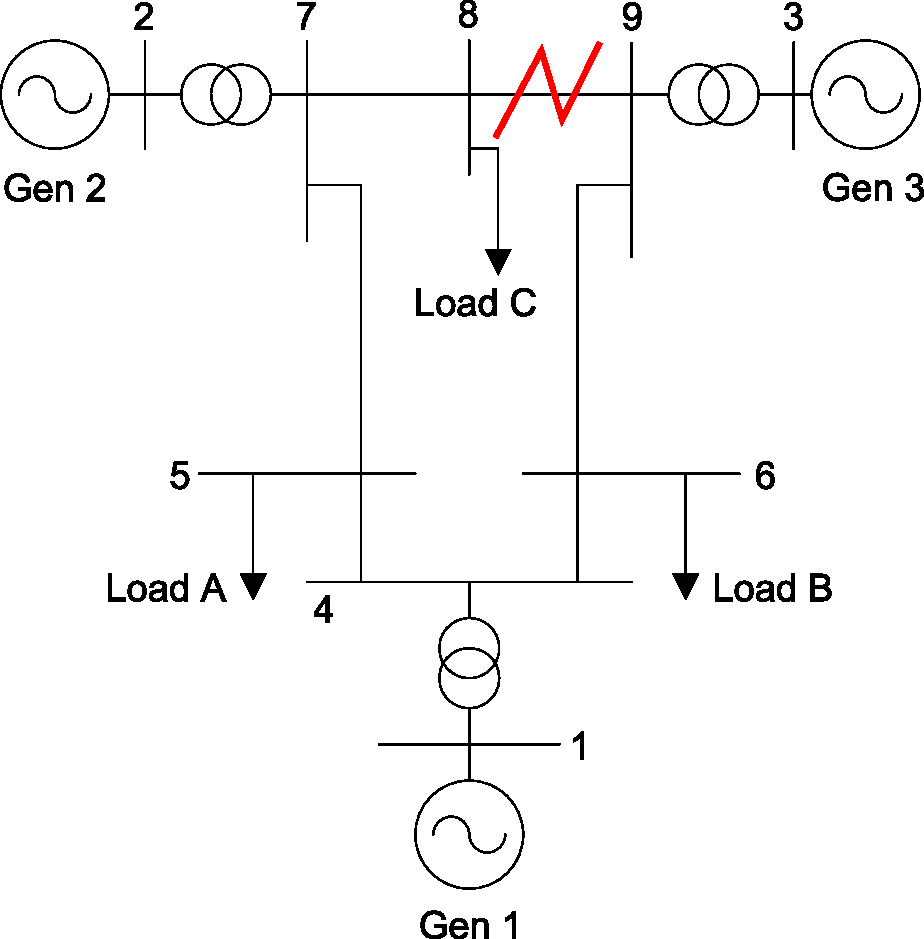
\includegraphics[width=\textwidth]{Figs/Ieee9bus_fault89.pdf}
\column{0.5\textwidth}
% This file was created by matlab2tikz v0.4.1.
% Copyright (c) 2008--2013, Nico Schlömer <nico.schloemer@gmail.com>
% All rights reserved.
% 
% The latest updates can be retrieved from
%   http://www.mathworks.com/matlabcentral/fileexchange/22022-matlab2tikz
% where you can also make suggestions and rate matlab2tikz.
% 
% 
% 
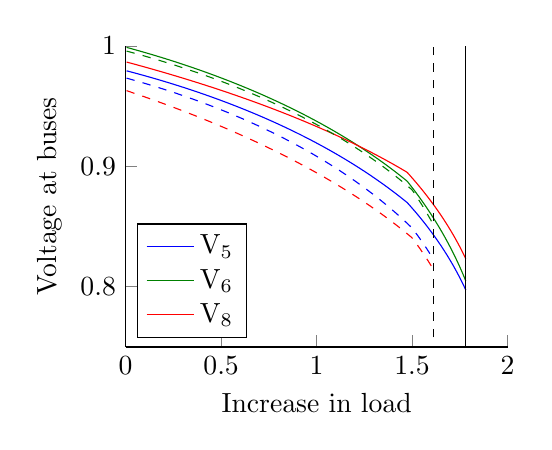
\begin{tikzpicture}

\begin{axis}[%
width=\fwidth,
height=0.788709677419355\fwidth,
scale only axis,
xmin=0,
xmax=2,
xlabel={Increase in load},
ymin=0.75,
ymax=1,
ylabel={Voltage at buses},
axis x line*=bottom,
axis y line*=left,
legend style={at={(0.03,0.03)},anchor=south west,draw=black,fill=white,legend cell align=left}
]
\addplot [
color=blue,
solid
]
table[row sep=crcr]{
0.005 0.979232052476942\\
0.01 0.97902472499685\\
0.015 0.978816627748652\\
0.02 0.978607758936801\\
0.025 0.978398116752672\\
0.03 0.978187699374455\\
0.035 0.977976504967064\\
0.04 0.977764531682033\\
0.045 0.977551777657413\\
0.05 0.977338241017672\\
0.055 0.977123919873591\\
0.06 0.976908812322158\\
0.065 0.976692916446462\\
0.07 0.976476230315584\\
0.075 0.976258751984497\\
0.08 0.97604047949394\\
0.085 0.975821410870326\\
0.09 0.975601544125613\\
0.095 0.975380877257204\\
0.1 0.975159408247819\\
0.105 0.974937135065394\\
0.11 0.974714055662948\\
0.115 0.974490167978475\\
0.12 0.97426546993482\\
0.125 0.974039959439555\\
0.13 0.973813634384864\\
0.135 0.97358649264741\\
0.14 0.973358532088208\\
0.145 0.973129750552511\\
0.15 0.972900145869665\\
0.155 0.972669715852988\\
0.16 0.972438458299638\\
0.165 0.972206370990475\\
0.17 0.971973451689931\\
0.175 0.971739698145868\\
0.18 0.971505108089446\\
0.185 0.971269679234981\\
0.19 0.971033409279799\\
0.195 0.9707962959041\\
0.2 0.970558336770811\\
0.205 0.970319529525434\\
0.21 0.970079871795907\\
0.215 0.969839361192448\\
0.22 0.969597995307403\\
0.225 0.969355771715097\\
0.23 0.96911268797167\\
0.235 0.968868741614931\\
0.24 0.96862393016419\\
0.245 0.968378251120101\\
0.25 0.968131701964495\\
0.255 0.967884280160218\\
0.26 0.967635983150967\\
0.265 0.967386808361114\\
0.27 0.967136753195537\\
0.275 0.966885815039451\\
0.28 0.966633991258225\\
0.285 0.966381279197213\\
0.29 0.966127676181567\\
0.295 0.965873179516057\\
0.3 0.965617786484891\\
0.305 0.965361494351521\\
0.31 0.965104300358459\\
0.315 0.964846201727088\\
0.32 0.964587195657461\\
0.325 0.96432727932811\\
0.33 0.964066449895848\\
0.335 0.963804704495564\\
0.34 0.963542040240023\\
0.345 0.96327845421966\\
0.35 0.963013943502367\\
0.355 0.962748505133287\\
0.36 0.962482136134595\\
0.365 0.962214833505284\\
0.37 0.961946594220946\\
0.375 0.961677415233546\\
0.38 0.9614072934712\\
0.385 0.961136225837946\\
0.39 0.96086420921351\\
0.395 0.960591240453077\\
0.4 0.960317316387048\\
0.405 0.960042433820804\\
0.41 0.959766589534459\\
0.415 0.959489780282617\\
0.42 0.959212002794118\\
0.425 0.958933253771787\\
0.43 0.958653529892179\\
0.435 0.958372827805316\\
0.44 0.958091144134421\\
0.445 0.957808475475659\\
0.45 0.95752481839786\\
0.455 0.957240169442246\\
0.46 0.956954525122153\\
0.465 0.956667881922752\\
0.47 0.956380236300759\\
0.475 0.956091584684149\\
0.48 0.955801923471864\\
0.485 0.955511249033509\\
0.49 0.955219557709055\\
0.495 0.954926845808539\\
0.5 0.954633109611744\\
0.505 0.95433834536789\\
0.51 0.954042549295318\\
0.515 0.953745717581161\\
0.52 0.953447846381022\\
0.525 0.953148931818643\\
0.53 0.952848969985562\\
0.535 0.952547956940778\\
0.54 0.952245888710402\\
0.545 0.951942761287309\\
0.55 0.951638570630777\\
0.555 0.951333312666132\\
0.56 0.951026983284377\\
0.565 0.950719578341824\\
0.57 0.950411093659716\\
0.575 0.950101525023845\\
0.58 0.949790868184165\\
0.585 0.949479118854398\\
0.59 0.949166272711636\\
0.595 0.948852325395935\\
0.6 0.948537272509908\\
0.605 0.948221109618302\\
0.61 0.947903832247581\\
0.615 0.947585435885496\\
0.62 0.947265915980647\\
0.625 0.946945267942044\\
0.63 0.946623487138658\\
0.635 0.946300568898964\\
0.64 0.945976508510484\\
0.645 0.945651301219311\\
0.65 0.945324942229641\\
0.655 0.944997426703284\\
0.66 0.944668749759176\\
0.665 0.944338906472882\\
0.67 0.944007891876088\\
0.675 0.943675700956093\\
0.68 0.943342328655279\\
0.685000000000001 0.943007769870591\\
0.690000000000001 0.942672019452993\\
0.695000000000001 0.94233507220693\\
0.700000000000001 0.941996922889765\\
0.705000000000001 0.941657566211222\\
0.710000000000001 0.941316996832811\\
0.715000000000001 0.940975209367252\\
0.720000000000001 0.94063219837788\\
0.725000000000001 0.940287958378049\\
0.730000000000001 0.939942483830522\\
0.735000000000001 0.939595769146855\\
0.740000000000001 0.939247808686765\\
0.745000000000001 0.938898596757493\\
0.750000000000001 0.938548127613157\\
0.755000000000001 0.938196395454092\\
0.760000000000001 0.937843394426179\\
0.765000000000001 0.937489118620167\\
0.770000000000001 0.937133562070975\\
0.775000000000001 0.936776718756997\\
0.780000000000001 0.93641858259938\\
0.785000000000001 0.936059147461303\\
0.790000000000001 0.935698407147235\\
0.795000000000001 0.935336355402183\\
0.800000000000001 0.934972985910932\\
0.805000000000001 0.934608292297266\\
0.810000000000001 0.93424226812318\\
0.815000000000001 0.933874906888075\\
0.820000000000001 0.933506202027946\\
0.825000000000001 0.933136146914546\\
0.830000000000001 0.932764734854547\\
0.835000000000001 0.932391959088675\\
0.840000000000001 0.932017812790845\\
0.845000000000001 0.931642289067262\\
0.850000000000001 0.931265380955526\\
0.855000000000001 0.930887081423705\\
0.860000000000001 0.930507383369403\\
0.865000000000001 0.930126279618808\\
0.870000000000001 0.929743762925718\\
0.875000000000001 0.929359825970559\\
0.880000000000001 0.928974461359383\\
0.885000000000001 0.928587661622839\\
0.890000000000001 0.928199419215138\\
0.895000000000001 0.927809726512996\\
0.900000000000001 0.927418575814553\\
0.905000000000001 0.927025959338274\\
0.910000000000001 0.926631869221839\\
0.915000000000001 0.926236297520995\\
0.920000000000001 0.925839236208407\\
0.925000000000001 0.925440677172475\\
0.930000000000001 0.925040612216129\\
0.935000000000001 0.924639033055613\\
0.940000000000001 0.924235931319227\\
0.945000000000001 0.923831298546071\\
0.950000000000001 0.923425126184737\\
0.955000000000001 0.923017405592005\\
0.960000000000001 0.922608128031487\\
0.965000000000001 0.922197284672269\\
0.970000000000001 0.921784866587509\\
0.975000000000001 0.921370864753017\\
0.980000000000001 0.920955270045811\\
0.985000000000001 0.920538073242635\\
0.990000000000001 0.920119265018455\\
0.995000000000001 0.919698835944925\\
1 0.919276776488821\\
1.005 0.918853077010446\\
1.01 0.918427727762004\\
1.015 0.91800071888594\\
1.02 0.917572040413243\\
1.025 0.917141682261728\\
1.03 0.916709634234268\\
1.035 0.916275886017003\\
1.04 0.9158404271775\\
1.045 0.915403247162889\\
1.05 0.914964335297953\\
1.055 0.914523680783177\\
1.06 0.914081272692762\\
1.065 0.913637099972596\\
1.07 0.913191151438185\\
1.075 0.912743415772529\\
1.08 0.912293881523976\\
1.085 0.911842537104001\\
1.09 0.911389370784969\\
1.095 0.910934370697825\\
1.1 0.91047752482975\\
1.105 0.910018821021757\\
1.11 0.909558246966245\\
1.115 0.909095790204486\\
1.12 0.908631438124073\\
1.125 0.908165177956298\\
1.13 0.907696996773481\\
1.135 0.907226881486238\\
1.14 0.906754818840685\\
1.145 0.906280795415581\\
1.15 0.90580479761941\\
1.155 0.905326811687392\\
1.16 0.904846823678429\\
1.165 0.90436481947198\\
1.17 0.903880784764868\\
1.175 0.903394705068004\\
1.18 0.902906565703046\\
1.185 0.902416351798974\\
1.19 0.901924048288587\\
1.195 0.901429639904913\\
1.2 0.900933111177543\\
1.20497298395187 0.900437146584785\\
1.20992526856465 0.899941131037016\\
1.21485696063708 0.899445064689713\\
1.21976816591341 0.898948947696048\\
1.22465898907991 0.898452780206842\\
1.22952953378013 0.897956562370589\\
1.23437990262991 0.897460294333487\\
1.23921019723211 0.896963976239474\\
1.2440205181911 0.896467608230245\\
1.24881096512691 0.895971190445292\\
1.25358163668918 0.895474723021924\\
1.25833263057079 0.894978206095298\\
1.26306404352137 0.894481639798445\\
1.26777597136041 0.893985024262295\\
1.27246850899021 0.893488359615704\\
1.27714175040859 0.89299164598548\\
1.28179578872141 0.892494883496404\\
1.28643071615476 0.89199807227126\\
1.29104662406705 0.891501212430853\\
1.29564360296083 0.891004304094036\\
1.30022174249439 0.890507347377731\\
1.30478113149316 0.890010342396953\\
1.30932185796096 0.889513289264831\\
1.31384400909099 0.88901618809263\\
1.31834767127666 0.888519038989772\\
1.32283293012223 0.888021842063856\\
1.32729987045327 0.887524597420682\\
1.33174857632692 0.887027305164266\\
1.336179131042 0.886529965396862\\
1.34059161714895 0.886032578218982\\
1.34498611645954 0.885535143729415\\
1.34936271005653 0.885037662025244\\
1.35372147830306 0.884540133201866\\
1.35806250085191 0.884042557353006\\
1.36238585665466 0.883544934570742\\
1.36669162397063 0.883047264945515\\
1.37097988037572 0.88254954856615\\
1.37525070277103 0.882051785519872\\
1.37950416739145 0.881553975892319\\
1.38374034981404 0.881056119767564\\
1.38795932496622 0.880558217228126\\
1.39216116713397 0.880060268354987\\
1.39634594996977 0.879562273227608\\
1.40051374650046 0.879064231923942\\
1.40466462913498 0.87856614452045\\
1.40879866967199 0.878068011092116\\
1.41291593930731 0.877569831712458\\
1.41701650864131 0.877071606453547\\
1.4211004476862 0.876573335386014\\
1.4251678258731 0.876075018579069\\
1.42921871205906 0.875576656100512\\
1.43325317453404 0.875078248016746\\
1.43727128102765 0.874579794392787\\
1.44127309871588 0.874081295292283\\
1.44525869422766 0.873582750777517\\
1.44922813365137 0.873084160909429\\
1.45318148254125 0.87258552574762\\
1.45711880592367 0.872086845350366\\
1.4610401683033 0.87158811977463\\
1.46494563366927 0.871089349076074\\
1.46883526550114 0.870590533309067\\
1.47270912677483 0.870091672526697\\
1.47579130221616 0.869628004653946\\
1.47829399300274 0.869190161405018\\
1.48078768860855 0.868752308829099\\
1.48327241224409 0.868314447007678\\
1.48574818699804 0.867876576022114\\
1.48821503583894 0.867438695953651\\
1.49067298161619 0.867000806883415\\
1.49312204706092 0.866562908892419\\
1.4955622547869 0.866125002061569\\
1.49799362729146 0.865687086471663\\
1.50041618695643 0.865249162203397\\
1.50282995604894 0.864811229337368\\
1.50523495672237 0.864373287954076\\
1.50763121101719 0.86393533813393\\
1.51001874086183 0.863497379957246\\
1.51239756807352 0.863059413504256\\
1.51476771435915 0.86262143885511\\
1.51712920131609 0.862183456089875\\
1.51948205043304 0.861745465288542\\
1.52182628309083 0.861307466531028\\
1.52416192056321 0.860869459897181\\
1.52648898401772 0.860431445466779\\
1.52880749451639 0.859993423319538\\
1.53111747301665 0.85955539353511\\
1.53341894037198 0.859117356193091\\
1.53571191733276 0.858679311373022\\
1.53799642454702 0.858241259154388\\
1.54027248256119 0.85780319961663\\
1.54254011182085 0.85736513283914\\
1.54479933267149 0.856927058901266\\
1.54705016535919 0.856488977882318\\
1.54929263003143 0.856050889861569\\
1.55152674673775 0.855612794918257\\
1.55375253543047 0.855174693131589\\
1.55597001596542 0.854736584580744\\
1.55817920810264 0.854298469344875\\
1.56038013150704 0.853860347503114\\
1.56257280574913 0.853422219134572\\
1.56475725030568 0.852984084318346\\
1.56693348456037 0.852545943133518\\
1.5691015278045 0.852107795659158\\
1.57126139923764 0.851669641974332\\
1.57341311796827 0.851231482158099\\
1.57555670301444 0.850793316289514\\
1.5776921733044 0.850355144447637\\
1.57981954767726 0.84991696671153\\
1.58193884488359 0.84947878316026\\
1.5840500835861 0.849040593872908\\
1.58615328236017 0.848602398928562\\
1.58824845969456 0.84816419840633\\
1.59033563399195 0.847725992385334\\
1.59241482356956 0.84728778094472\\
1.59448604665977 0.846849564163657\\
1.59654932141069 0.846411342121339\\
1.59860466588672 0.845973114896991\\
1.60065209806919 0.845534882569871\\
1.6026916358569 0.845096645219269\\
1.60472329706666 0.844658402924514\\
1.60674709943393 0.844220155764978\\
1.60876306061331 0.843781903820073\\
1.61077119817912 0.843343647169259\\
1.61277152962596 0.842905385892045\\
1.61476407236924 0.842467120067991\\
1.61674884374571 0.842028849776711\\
1.61872586101402 0.841590575097877\\
1.62069514135523 0.841152296111222\\
1.62265670187335 0.840714012896541\\
1.62461055959583 0.840275725533693\\
1.62655673147413 0.839837434102608\\
1.62849523438416 0.839399138683286\\
1.63042608512686 0.8389608393558\\
1.63234930042862 0.8385225362003\\
1.63426489694185 0.838084229297017\\
1.63617289124547 0.837645918726263\\
1.63807329984532 0.837207604568434\\
1.63996613917473 0.836769286904015\\
1.64185142559497 0.836330965813581\\
1.64372917539571 0.8358926413778\\
1.6455994047955 0.835454313677436\\
1.64746212994226 0.835015982793352\\
1.64931736691372 0.834577648806512\\
1.65116513171786 0.834139311797985\\
1.65300544029344 0.833700971848945\\
1.65483830851035 0.833262629040678\\
1.65666375217014 0.832824283454581\\
1.65848178700643 0.832385935172168\\
1.66029242868532 0.831947584275069\\
1.6620956928059 0.831509230845035\\
1.66389159490061 0.831070874963942\\
1.66568015043572 0.830632516713791\\
1.6674613748117 0.830194156176713\\
1.6692352833637 0.82975579343497\\
1.67100189136193 0.829317428570958\\
1.67276121401209 0.828879061667212\\
1.67451326645577 0.828440692806407\\
1.67625806377087 0.82800232207136\\
1.67799562097198 0.827563949545034\\
1.6797259530108 0.827125575310542\\
1.68144907477654 0.826687199451146\\
1.68316500109629 0.826248822050264\\
1.68487374673544 0.82581044319147\\
1.68657532639803 0.825372062958497\\
1.68826975472718 0.824933681435243\\
1.68995704630543 0.82449529870577\\
1.69163721565512 0.824056914854306\\
1.69331027723879 0.823618529965256\\
1.69497624545954 0.823180144123192\\
1.69663513466137 0.822741757412867\\
1.69828695912959 0.822303369919213\\
1.69993173309116 0.821864981727342\\
1.70156947071501 0.821426592922556\\
1.70320018611249 0.82098820359034\\
1.70482389333761 0.820549813816373\\
1.70644060638749 0.820111423686527\\
1.70805033920263 0.819673033286871\\
1.70965310566729 0.819234642703675\\
1.71124891960986 0.818796252023408\\
1.7128377948031 0.818357861332748\\
1.71441974496461 0.81791947071858\\
1.71599478375704 0.817481080267999\\
1.71756292478849 0.817042690068318\\
1.71912418161284 0.816604300207063\\
1.72067856773003 0.816165910771982\\
1.7222260965864 0.815727521851048\\
1.72376678157505 0.815289133532456\\
1.72530063603609 0.814850745904633\\
1.726827673257 0.814412359056236\\
1.72834790647294 0.81397397307616\\
1.72986134886702 0.813535588053534\\
1.73136801357067 0.813097204077732\\
1.73286791366386 0.812658821238369\\
1.73436106217552 0.812220439625308\\
1.7358474720837 0.811782059328663\\
1.73732715631597 0.8113436804388\\
1.73880012774968 0.810905303046343\\
1.74026639921226 0.810466927242172\\
1.7417259834815 0.810028553117432\\
1.74317889328582 0.809590180763534\\
1.7446251413046 0.809151810272155\\
1.74606474016843 0.808713441735246\\
1.7474977024594 0.808275075245032\\
1.74892404071139 0.807836710894016\\
1.75034376741033 0.807398348774981\\
1.75175689499446 0.806959988980998\\
1.75316343585465 0.80652163160542\\
1.75456340233463 0.806083276741896\\
1.75595680673126 0.805644924484365\\
1.75734366129481 0.805206574927065\\
1.75872397822922 0.804768228164535\\
1.76009776969238 0.804329884291616\\
1.76146504779632 0.803891543403457\\
1.76282582460756 0.803453205595516\\
1.76418011214731 0.803014870963566\\
1.76552792239173 0.802576539603695\\
1.76686926727219 0.802138211612313\\
1.76820415867552 0.801699887086152\\
1.76953260844424 0.801261566122271\\
1.77085462837683 0.80082324881806\\
1.77217023022798 0.800384935271242\\
1.77347942570878 0.799946625579877\\
1.77478222648702 0.799508319842363\\
1.7760786441874 0.799070018157447\\
1.77736869039176 0.798631720624219\\
1.77865237663933 0.798193427342121\\
1.77992971442697 0.797755138410948\\
1.78120071520936 0.797316853930855\\
};
\addlegendentry{$\text{V}_\text{5}$};

\addplot [
color=green!50!black,
solid
]
table[row sep=crcr]{
0.005 0.998686038128165\\
0.01 0.998470807513519\\
0.015 0.998254815896074\\
0.02 0.998038061500132\\
0.025 0.997820542537159\\
0.03 0.997602257205685\\
0.035 0.997383203691213\\
0.04 0.997163380166114\\
0.045 0.996942784789531\\
0.05 0.996721415707276\\
0.055 0.996499271051735\\
0.06 0.996276348941757\\
0.065 0.996052647482554\\
0.07 0.995828164765599\\
0.075 0.995602898868513\\
0.08 0.995376847854963\\
0.085 0.995150009774552\\
0.09 0.994922382662708\\
0.095 0.994693964540574\\
0.1 0.994464753414892\\
0.105 0.9942347472779\\
0.11 0.994003944107203\\
0.115 0.993772341865665\\
0.12 0.993539938501291\\
0.125 0.993306731947106\\
0.13 0.993072720121036\\
0.135 0.992837900925786\\
0.14 0.992602272248714\\
0.145 0.992365831961713\\
0.15 0.992128577921079\\
0.155 0.991890507967386\\
0.16 0.991651619925355\\
0.165 0.99141191160373\\
0.17 0.991171380795137\\
0.175 0.990930025275956\\
0.18 0.990687842806186\\
0.185 0.990444831129306\\
0.19 0.990200987972138\\
0.195 0.989956311044708\\
0.2 0.989710798040102\\
0.205 0.989464446634324\\
0.21 0.989217254486153\\
0.215 0.988969219236992\\
0.22 0.988720338510728\\
0.225 0.988470609913568\\
0.23 0.9882200310339\\
0.235 0.987968599442133\\
0.24 0.987716312690542\\
0.245 0.987463168313114\\
0.25 0.987209163825381\\
0.255 0.986954296724267\\
0.26 0.98669856448792\\
0.265 0.986441964575546\\
0.27 0.986184494427244\\
0.275 0.985926151463838\\
0.28 0.9856669330867\\
0.285 0.985406836677582\\
0.29 0.985145859598439\\
0.295 0.984883999191248\\
0.3 0.984621252777832\\
0.305 0.984357617659675\\
0.31 0.98409309111774\\
0.315 0.983827670412279\\
0.32 0.983561352782646\\
0.325 0.983294135447103\\
0.33 0.983026015602632\\
0.335 0.982756990424732\\
0.34 0.982487057067221\\
0.345 0.982216212662041\\
0.35 0.981944454319044\\
0.355 0.981671779125794\\
0.36 0.981398184147355\\
0.365 0.981123666426076\\
0.37 0.980848222981382\\
0.375 0.980571850809553\\
0.38 0.980294546883505\\
0.385 0.980016308152566\\
0.39 0.979737131542254\\
0.395 0.979457013954042\\
0.4 0.979175952265133\\
0.405 0.97889394332822\\
0.41 0.978610983971251\\
0.415 0.978327070997188\\
0.42 0.978042201183761\\
0.425 0.977756371283223\\
0.43 0.977469578022098\\
0.435 0.97718181810093\\
0.44 0.976893088194018\\
0.445 0.976603384949168\\
0.45 0.976312704987417\\
0.455 0.97602104490277\\
0.46 0.975728401261932\\
0.465 0.975434770604026\\
0.47 0.975140149440322\\
0.475 0.974844534253947\\
0.48 0.974547921499608\\
0.485 0.97425030760329\\
0.49 0.973951688961974\\
0.495 0.973652061943331\\
0.5 0.973351422885422\\
0.505 0.973049768096394\\
0.51 0.972747093854166\\
0.515 0.972443396406114\\
0.52 0.972138671968755\\
0.525 0.971832916727424\\
0.53 0.971526126835937\\
0.535 0.971218298416271\\
0.54 0.970909427558217\\
0.545 0.97059951031904\\
0.55 0.970288542723136\\
0.555 0.969976520761674\\
0.56 0.969663440392244\\
0.565 0.96934929753849\\
0.57 0.96903408808975\\
0.575 0.968717807900674\\
0.58 0.968400452790854\\
0.585 0.968082018544437\\
0.59 0.967762500909739\\
0.595 0.967441895598846\\
0.6 0.967120198287216\\
0.605 0.966797404613275\\
0.61 0.966473510178001\\
0.615 0.966148510544509\\
0.62 0.965822401237626\\
0.625 0.965495177743459\\
0.63 0.965166835508959\\
0.635 0.964837369941478\\
0.64 0.964506776408318\\
0.645 0.964175050236276\\
0.65 0.963842186711176\\
0.655 0.963508181077405\\
0.66 0.963173028537426\\
0.665 0.962836724251306\\
0.67 0.962499263336208\\
0.675 0.962160640865904\\
0.68 0.96182085187026\\
0.685000000000001 0.961479891334724\\
0.690000000000001 0.961137754199798\\
0.695000000000001 0.960794435360515\\
0.700000000000001 0.96044992966589\\
0.705000000000001 0.960104231918377\\
0.710000000000001 0.959757336873312\\
0.715000000000001 0.959409239238344\\
0.720000000000001 0.959059933672865\\
0.725000000000001 0.958709414787425\\
0.730000000000001 0.958357677143137\\
0.735000000000001 0.95800471525108\\
0.740000000000001 0.957650523571678\\
0.745000000000001 0.95729509651409\\
0.750000000000001 0.95693842843557\\
0.755000000000001 0.956580513640829\\
0.760000000000001 0.95622134638138\\
0.765000000000001 0.955860920854878\\
0.770000000000001 0.955499231204446\\
0.775000000000001 0.955136271517989\\
0.780000000000001 0.954772035827498\\
0.785000000000001 0.954406518108345\\
0.790000000000001 0.954039712278562\\
0.795000000000001 0.95367161219811\\
0.800000000000001 0.953302211668138\\
0.805000000000001 0.952931504430224\\
0.810000000000001 0.952559484165609\\
0.815000000000001 0.952186144494416\\
0.820000000000001 0.951811478974857\\
0.825000000000001 0.951435481102418\\
0.830000000000001 0.951058144309046\\
0.835000000000001 0.95067946196231\\
0.840000000000001 0.950299427364549\\
0.845000000000001 0.949918033752009\\
0.850000000000001 0.949535274293966\\
0.855000000000001 0.949151142091824\\
0.860000000000001 0.948765630178213\\
0.865000000000001 0.948378731516058\\
0.870000000000001 0.947990438997632\\
0.875000000000001 0.947600745443607\\
0.880000000000001 0.94720964360207\\
0.885000000000001 0.946817126147532\\
0.890000000000001 0.946423185679912\\
0.895000000000001 0.946027814723517\\
0.900000000000001 0.945631005725988\\
0.905000000000001 0.945232751057228\\
0.910000000000001 0.944833043008327\\
0.915000000000001 0.944431873790448\\
0.920000000000001 0.944029235533704\\
0.925000000000001 0.943625120286008\\
0.930000000000001 0.943219520011909\\
0.935000000000001 0.9428124265914\\
0.940000000000001 0.942403831818708\\
0.945000000000001 0.941993727401055\\
0.950000000000001 0.941582104957407\\
0.955000000000001 0.941168956017191\\
0.960000000000001 0.940754272018985\\
0.965000000000001 0.940338044309195\\
0.970000000000001 0.939920264140697\\
0.975000000000001 0.93950092267145\\
0.980000000000001 0.939080010963102\\
0.985000000000001 0.93865751997954\\
0.990000000000001 0.938233440585439\\
0.995000000000001 0.937807763544761\\
1 0.937380479519245\\
1.005 0.936951579066849\\
1.01 0.936521052640174\\
1.015 0.93608889058485\\
1.02 0.935655083137893\\
1.025 0.935219620426027\\
1.03 0.934782492463977\\
1.035 0.93434368915272\\
1.04 0.933903200277709\\
1.045 0.933461015507054\\
1.05 0.933017124389671\\
1.055 0.932571516353387\\
1.06 0.932124180703016\\
1.065 0.931675106618382\\
1.07 0.931224283152313\\
1.075 0.930771699228586\\
1.08 0.93031734363983\\
1.085 0.929861205045387\\
1.09 0.929403271969127\\
1.095 0.928943532797212\\
1.1 0.928481975775821\\
1.105 0.928018589008819\\
1.11 0.927553360455379\\
1.115 0.927086277927544\\
1.12 0.926617329087758\\
1.125 0.926146501446313\\
1.13 0.925673782358763\\
1.135 0.925199159023272\\
1.14 0.924722618477902\\
1.145 0.924244147597843\\
1.15 0.923763733092579\\
1.155 0.923281361502994\\
1.16 0.922797019198407\\
1.165 0.922310692373541\\
1.17 0.92182236704543\\
1.175 0.921332029050237\\
1.18 0.920839664040022\\
1.185 0.920345257479411\\
1.19 0.919848794642212\\
1.195 0.919350260607925\\
1.2 0.918849640258189\\
1.20497298395187 0.918349640258189\\
1.20992526856465 0.917849640258189\\
1.21485696063708 0.91734964025819\\
1.21976816591341 0.91684964025819\\
1.22465898907991 0.91634964025819\\
1.22952953378013 0.91584964025819\\
1.23437990262991 0.91534964025819\\
1.23921019723211 0.91484964025819\\
1.2440205181911 0.91434964025819\\
1.24881096512691 0.91384964025819\\
1.25358163668918 0.91334964025819\\
1.25833263057079 0.912849640258191\\
1.26306404352137 0.912349640258191\\
1.26777597136041 0.911849640258191\\
1.27246850899021 0.911349640258191\\
1.27714175040859 0.910849640258191\\
1.28179578872141 0.910349640258191\\
1.28643071615476 0.909849640258191\\
1.29104662406705 0.909349640258191\\
1.29564360296083 0.908849640258191\\
1.30022174249439 0.908349640258191\\
1.30478113149316 0.907849640258192\\
1.30932185796096 0.907349640258192\\
1.31384400909099 0.906849640258192\\
1.31834767127666 0.906349640258192\\
1.32283293012223 0.905849640258192\\
1.32729987045327 0.905349640258192\\
1.33174857632692 0.904849640258192\\
1.336179131042 0.904349640258192\\
1.34059161714895 0.903849640258192\\
1.34498611645954 0.903349640258192\\
1.34936271005653 0.902849640258192\\
1.35372147830306 0.902349640258192\\
1.35806250085191 0.901849640258192\\
1.36238585665466 0.901349640258192\\
1.36669162397063 0.900849640258192\\
1.37097988037572 0.900349640258192\\
1.37525070277103 0.899849640258192\\
1.37950416739145 0.899349640258192\\
1.38374034981404 0.898849640258192\\
1.38795932496622 0.898349640258192\\
1.39216116713397 0.897849640258192\\
1.39634594996977 0.897349640258193\\
1.40051374650046 0.896849640258193\\
1.40466462913498 0.896349640258193\\
1.40879866967199 0.895849640258193\\
1.41291593930731 0.895349640258193\\
1.41701650864131 0.894849640258193\\
1.4211004476862 0.894349640258193\\
1.4251678258731 0.893849640258193\\
1.42921871205906 0.893349640258193\\
1.43325317453404 0.892849640258193\\
1.43727128102765 0.892349640258193\\
1.44127309871588 0.891849640258193\\
1.44525869422766 0.891349640258193\\
1.44922813365137 0.890849640258193\\
1.45318148254125 0.890349640258193\\
1.45711880592367 0.889849640258193\\
1.4610401683033 0.889349640258193\\
1.46494563366927 0.888849640258193\\
1.46883526550114 0.888349640258193\\
1.47270912677483 0.887849640258193\\
1.47579130221616 0.887349640258193\\
1.47829399300274 0.886849640258193\\
1.48078768860855 0.886349640258193\\
1.48327241224409 0.885849640258193\\
1.48574818699804 0.885349640258193\\
1.48821503583894 0.884849640258193\\
1.49067298161619 0.884349640258194\\
1.49312204706092 0.883849640258194\\
1.4955622547869 0.883349640258194\\
1.49799362729146 0.882849640258194\\
1.50041618695643 0.882349640258194\\
1.50282995604894 0.881849640258194\\
1.50523495672237 0.881349640258194\\
1.50763121101719 0.880849640258194\\
1.51001874086183 0.880349640258194\\
1.51239756807352 0.879849640258194\\
1.51476771435915 0.879349640258194\\
1.51712920131609 0.878849640258194\\
1.51948205043304 0.878349640258194\\
1.52182628309083 0.877849640258194\\
1.52416192056321 0.877349640258195\\
1.52648898401772 0.876849640258195\\
1.52880749451639 0.876349640258195\\
1.53111747301665 0.875849640258195\\
1.53341894037198 0.875349640258195\\
1.53571191733276 0.874849640258195\\
1.53799642454702 0.874349640258195\\
1.54027248256119 0.873849640258195\\
1.54254011182085 0.873349640258195\\
1.54479933267149 0.872849640258195\\
1.54705016535919 0.872349640258195\\
1.54929263003143 0.871849640258195\\
1.55152674673775 0.871349640258196\\
1.55375253543047 0.870849640258195\\
1.55597001596542 0.870349640258196\\
1.55817920810264 0.869849640258196\\
1.56038013150704 0.869349640258196\\
1.56257280574913 0.868849640258196\\
1.56475725030568 0.868349640258196\\
1.56693348456037 0.867849640258196\\
1.5691015278045 0.867349640258196\\
1.57126139923764 0.866849640258196\\
1.57341311796827 0.866349640258196\\
1.57555670301444 0.865849640258196\\
1.5776921733044 0.865349640258196\\
1.57981954767726 0.864849640258196\\
1.58193884488359 0.864349640258196\\
1.5840500835861 0.863849640258196\\
1.58615328236017 0.863349640258196\\
1.58824845969456 0.862849640258197\\
1.59033563399195 0.862349640258197\\
1.59241482356956 0.861849640258197\\
1.59448604665977 0.861349640258197\\
1.59654932141069 0.860849640258197\\
1.59860466588672 0.860349640258197\\
1.60065209806919 0.859849640258197\\
1.6026916358569 0.859349640258197\\
1.60472329706666 0.858849640258197\\
1.60674709943393 0.858349640258197\\
1.60876306061331 0.857849640258197\\
1.61077119817912 0.857349640258197\\
1.61277152962596 0.856849640258197\\
1.61476407236924 0.856349640258197\\
1.61674884374571 0.855849640258197\\
1.61872586101402 0.855349640258197\\
1.62069514135523 0.854849640258197\\
1.62265670187335 0.854349640258197\\
1.62461055959583 0.853849640258198\\
1.62655673147413 0.853349640258198\\
1.62849523438416 0.852849640258198\\
1.63042608512686 0.852349640258198\\
1.63234930042862 0.851849640258198\\
1.63426489694185 0.851349640258198\\
1.63617289124547 0.850849640258198\\
1.63807329984532 0.850349640258198\\
1.63996613917473 0.849849640258198\\
1.64185142559497 0.849349640258198\\
1.64372917539571 0.848849640258198\\
1.6455994047955 0.848349640258198\\
1.64746212994226 0.847849640258198\\
1.64931736691372 0.847349640258198\\
1.65116513171786 0.846849640258198\\
1.65300544029344 0.846349640258198\\
1.65483830851035 0.845849640258198\\
1.65666375217014 0.845349640258198\\
1.65848178700643 0.844849640258199\\
1.66029242868532 0.844349640258199\\
1.6620956928059 0.843849640258199\\
1.66389159490061 0.843349640258199\\
1.66568015043572 0.842849640258199\\
1.6674613748117 0.842349640258199\\
1.6692352833637 0.841849640258199\\
1.67100189136193 0.841349640258199\\
1.67276121401209 0.840849640258199\\
1.67451326645577 0.840349640258199\\
1.67625806377087 0.8398496402582\\
1.67799562097198 0.8393496402582\\
1.6797259530108 0.8388496402582\\
1.68144907477654 0.8383496402582\\
1.68316500109629 0.8378496402582\\
1.68487374673544 0.8373496402582\\
1.68657532639803 0.8368496402582\\
1.68826975472718 0.8363496402582\\
1.68995704630543 0.8358496402582\\
1.69163721565512 0.8353496402582\\
1.69331027723879 0.8348496402582\\
1.69497624545954 0.8343496402582\\
1.69663513466137 0.8338496402582\\
1.69828695912959 0.8333496402582\\
1.69993173309116 0.8328496402582\\
1.70156947071501 0.8323496402582\\
1.70320018611249 0.8318496402582\\
1.70482389333761 0.8313496402582\\
1.70644060638749 0.8308496402582\\
1.70805033920263 0.8303496402582\\
1.70965310566729 0.8298496402582\\
1.71124891960986 0.8293496402582\\
1.7128377948031 0.828849640258201\\
1.71441974496461 0.828349640258201\\
1.71599478375704 0.827849640258201\\
1.71756292478849 0.827349640258201\\
1.71912418161284 0.826849640258201\\
1.72067856773003 0.826349640258201\\
1.7222260965864 0.825849640258201\\
1.72376678157505 0.825349640258201\\
1.72530063603609 0.824849640258201\\
1.726827673257 0.824349640258201\\
1.72834790647294 0.823849640258201\\
1.72986134886702 0.823349640258201\\
1.73136801357067 0.822849640258201\\
1.73286791366386 0.822349640258201\\
1.73436106217552 0.821849640258201\\
1.7358474720837 0.821349640258201\\
1.73732715631597 0.820849640258201\\
1.73880012774968 0.820349640258201\\
1.74026639921226 0.819849640258201\\
1.7417259834815 0.819349640258201\\
1.74317889328582 0.818849640258202\\
1.7446251413046 0.818349640258202\\
1.74606474016843 0.817849640258202\\
1.7474977024594 0.817349640258202\\
1.74892404071139 0.816849640258202\\
1.75034376741033 0.816349640258202\\
1.75175689499446 0.815849640258202\\
1.75316343585465 0.815349640258202\\
1.75456340233463 0.814849640258202\\
1.75595680673126 0.814349640258202\\
1.75734366129481 0.813849640258202\\
1.75872397822922 0.813349640258202\\
1.76009776969238 0.812849640258202\\
1.76146504779632 0.812349640258202\\
1.76282582460756 0.811849640258202\\
1.76418011214731 0.811349640258202\\
1.76552792239173 0.810849640258202\\
1.76686926727219 0.810349640258202\\
1.76820415867552 0.809849640258202\\
1.76953260844424 0.809349640258202\\
1.77085462837683 0.808849640258203\\
1.77217023022798 0.808349640258203\\
1.77347942570878 0.807849640258203\\
1.77478222648702 0.807349640258203\\
1.7760786441874 0.806849640258203\\
1.77736869039176 0.806349640258203\\
1.77865237663933 0.805849640258203\\
1.77992971442697 0.805349640258203\\
1.78120071520936 0.804849640258203\\
};
\addlegendentry{$\text{V}_\text{6}$};

\addplot [
color=red,
solid
]
table[row sep=crcr]{
0.005 0.986518903809878\\
0.01 0.986306414354071\\
0.015 0.986093465368436\\
0.02 0.985880055702197\\
0.025 0.985666184196952\\
0.03 0.985451849686603\\
0.035 0.985237050997311\\
0.04 0.985021786947427\\
0.045 0.984806056347438\\
0.05 0.984589857999902\\
0.055 0.984373190699396\\
0.06 0.984156053232445\\
0.065 0.983938444377469\\
0.07 0.983720362904712\\
0.075 0.983501807576185\\
0.08 0.983282777145597\\
0.085 0.983063270358294\\
0.09 0.982843285951195\\
0.095 0.982622822652718\\
0.1 0.982401879182721\\
0.105 0.982180454252433\\
0.11 0.98195854656438\\
0.115 0.981736154812322\\
0.12 0.981513277681182\\
0.125 0.98128991384697\\
0.13 0.98106606197672\\
0.135 0.980841720728411\\
0.14 0.980616888750893\\
0.145 0.980391564683822\\
0.15 0.980165747157573\\
0.155 0.979939434793175\\
0.16 0.979712626202224\\
0.165 0.979485319986816\\
0.17 0.979257514739463\\
0.175 0.979029209043012\\
0.18 0.978800401470568\\
0.185 0.978571090585416\\
0.19 0.97834127494093\\
0.195 0.978110953080498\\
0.2 0.977880123537435\\
0.205 0.977648784834898\\
0.21 0.9774169354858\\
0.215 0.977184573992724\\
0.22 0.976951698847835\\
0.225 0.976718308532789\\
0.23 0.976484401518647\\
0.235 0.97624997626578\\
0.24 0.976015031223777\\
0.245 0.975779564831356\\
0.25 0.975543575516264\\
0.255 0.975307061695187\\
0.26 0.975070021773648\\
0.265 0.974832454145913\\
0.27 0.974594357194891\\
0.275 0.974355729292033\\
0.28 0.974116568797232\\
0.285 0.97387687405872\\
0.29 0.973636643412963\\
0.295 0.973395875184558\\
0.3 0.973154567686125\\
0.305 0.9729127192182\\
0.31 0.972670328069125\\
0.315 0.972427392514941\\
0.32 0.972183910819273\\
0.325 0.971939881233215\\
0.33 0.971695301995223\\
0.335 0.971450171330992\\
0.34 0.971204487453341\\
0.345 0.970958248562098\\
0.35 0.970711452843971\\
0.355 0.970464098472436\\
0.36 0.970216183607609\\
0.365 0.969967706396118\\
0.37 0.969718664970984\\
0.375 0.969469057451487\\
0.38 0.969218881943041\\
0.385 0.968968136537058\\
0.39 0.968716819310817\\
0.395 0.968464928327333\\
0.4 0.968212461635213\\
0.405 0.967959417268525\\
0.41 0.967705793246657\\
0.415 0.96745158757417\\
0.42 0.96719679824066\\
0.425 0.966941423220611\\
0.43 0.966685460473246\\
0.435 0.966428907942383\\
0.44 0.966171763556277\\
0.445 0.965914025227469\\
0.45 0.965655690852637\\
0.455 0.965396758312426\\
0.46 0.965137225471305\\
0.465 0.964877090177389\\
0.47 0.964616350262289\\
0.475 0.964355003540938\\
0.48 0.964093047811426\\
0.485 0.96383048085483\\
0.49 0.96356730043504\\
0.495 0.963303504298586\\
0.5 0.96303909017446\\
0.505 0.962774055773935\\
0.51 0.962508398790386\\
0.515 0.962242116899102\\
0.52 0.961975207757101\\
0.525 0.96170766900294\\
0.53 0.961439498256522\\
0.535 0.961170693118903\\
0.54 0.960901251172091\\
0.545 0.960631169978851\\
0.55 0.960360447082493\\
0.555 0.960089080006677\\
0.56 0.959817066255194\\
0.565 0.959544403311761\\
0.57 0.959271088639803\\
0.575 0.958997119682236\\
0.58 0.958722493861245\\
0.585 0.958447208578062\\
0.59 0.958171261212734\\
0.595 0.957894649123901\\
0.6 0.95761736964855\\
0.605 0.95733942010179\\
0.61 0.957060797776601\\
0.615 0.956781499943598\\
0.62 0.956501523850775\\
0.625 0.956220866723261\\
0.63 0.955939525763062\\
0.635 0.955657498148799\\
0.64 0.955374781035451\\
0.645 0.955091371554084\\
0.65 0.954807266811581\\
0.655 0.954522463890369\\
0.66 0.95423695984814\\
0.665 0.953950751717566\\
0.67 0.953663836506013\\
0.675 0.953376211195253\\
0.68 0.953087872741161\\
0.685000000000001 0.952798818073419\\
0.690000000000001 0.952509044095212\\
0.695000000000001 0.952218547682914\\
0.700000000000001 0.951927325685779\\
0.705000000000001 0.951635374925616\\
0.710000000000001 0.951342692196468\\
0.715000000000001 0.951049274264282\\
0.720000000000001 0.950755117866576\\
0.725000000000001 0.950460219712096\\
0.730000000000001 0.950164576480474\\
0.735000000000001 0.949868184821875\\
0.740000000000001 0.949571041356644\\
0.745000000000001 0.949273142674942\\
0.750000000000001 0.94897448533638\\
0.755000000000001 0.948675065869643\\
0.760000000000001 0.948374880772116\\
0.765000000000001 0.948073926509492\\
0.770000000000001 0.947772199515387\\
0.775000000000001 0.947469696190939\\
0.780000000000001 0.947166412904399\\
0.785000000000001 0.946862345990731\\
0.790000000000001 0.946557491751183\\
0.795000000000001 0.946251846452869\\
0.800000000000001 0.945945406328337\\
0.805000000000001 0.945638167575126\\
0.810000000000001 0.945330126355326\\
0.815000000000001 0.945021278795119\\
0.820000000000001 0.944711620984321\\
0.825000000000001 0.944401148975914\\
0.830000000000001 0.944089858785565\\
0.835000000000001 0.943777746391144\\
0.840000000000001 0.943464807732235\\
0.845000000000001 0.943151038709626\\
0.850000000000001 0.942836435184805\\
0.855000000000001 0.942520992979438\\
0.860000000000001 0.942204707874844\\
0.865000000000001 0.941887575611457\\
0.870000000000001 0.941569591888278\\
0.875000000000001 0.941250752362321\\
0.880000000000001 0.940931052648048\\
0.885000000000001 0.940610488316789\\
0.890000000000001 0.940289054896163\\
0.895000000000001 0.939966747869478\\
0.900000000000001 0.939643562675123\\
0.905000000000001 0.939319494705954\\
0.910000000000001 0.938994539308662\\
0.915000000000001 0.938668691783134\\
0.920000000000001 0.938341947381803\\
0.925000000000001 0.938014301308985\\
0.930000000000001 0.937685748720196\\
0.935000000000001 0.937356284721477\\
0.940000000000001 0.937025904368681\\
0.945000000000001 0.936694602666765\\
0.950000000000001 0.936362374569065\\
0.955000000000001 0.936029214976551\\
0.960000000000001 0.935695118737077\\
0.965000000000001 0.93536008064461\\
0.970000000000001 0.935024095438446\\
0.975000000000001 0.934687157802417\\
0.980000000000001 0.934349262364072\\
0.985000000000001 0.934010403693855\\
0.990000000000001 0.933670576304254\\
0.995000000000001 0.933329774648945\\
1 0.932987993121914\\
1.005 0.932645226056561\\
1.01 0.932301467724788\\
1.015 0.931956712336072\\
1.02 0.931610954036512\\
1.025 0.931264186907869\\
1.03 0.930916404966574\\
1.035 0.930567602162724\\
1.04 0.930217772379057\\
1.045 0.929866909429903\\
1.05 0.929515007060121\\
1.055 0.929162058944003\\
1.06 0.928808058684166\\
1.065 0.928452999810416\\
1.07 0.928096875778594\\
1.075 0.927739679969385\\
1.08 0.927381405687122\\
1.085 0.927022046158545\\
1.09 0.926661594531548\\
1.095 0.926300043873895\\
1.1 0.925937387171903\\
1.105 0.925573617329111\\
1.11 0.925208727164906\\
1.115 0.924842709413122\\
1.12 0.924475556720623\\
1.125 0.92410726164583\\
1.13 0.923737816657245\\
1.135 0.923367214131913\\
1.14 0.922995446353874\\
1.145 0.922622505512571\\
1.15 0.922248383701218\\
1.155 0.921873072915138\\
1.16 0.921496565050065\\
1.165 0.921118851900401\\
1.17 0.920739925157439\\
1.175 0.92035977640754\\
1.18 0.919978397130277\\
1.185 0.919595778696522\\
1.19 0.919211912366508\\
1.195 0.918826789287825\\
1.2 0.918440400493383\\
1.20497298395187 0.918054834967705\\
1.20992526856465 0.917669612121599\\
1.21485696063708 0.917284730398044\\
1.21976816591341 0.916900188257588\\
1.22465898907991 0.916515984178527\\
1.22952953378013 0.916132116656646\\
1.23437990262991 0.915748584204969\\
1.23921019723211 0.915365385353506\\
1.2440205181911 0.914982518649014\\
1.24881096512691 0.914599982654752\\
1.25358163668918 0.914217775950249\\
1.25833263057079 0.913835897131071\\
1.26306404352137 0.913454344808601\\
1.26777597136041 0.913073117609805\\
1.27246850899021 0.912692214177025\\
1.27714175040859 0.91231163316776\\
1.28179578872141 0.911931373254453\\
1.28643071615476 0.911551433124289\\
1.29104662406705 0.911171811478991\\
1.29564360296083 0.910792507034617\\
1.30022174249439 0.91041351852137\\
1.30478113149316 0.910034844683401\\
1.30932185796096 0.909656484278624\\
1.31384400909099 0.909278436078525\\
1.31834767127666 0.908900698867988\\
1.32283293012223 0.908523271445107\\
1.32729987045327 0.908146152621018\\
1.33174857632692 0.90776934121972\\
1.336179131042 0.907392836077909\\
1.34059161714895 0.907016636044806\\
1.34498611645954 0.906640739982002\\
1.34936271005653 0.906265146763287\\
1.35372147830306 0.905889855274497\\
1.35806250085191 0.905514864413357\\
1.36238585665466 0.905140173089325\\
1.36669162397063 0.904765780223449\\
1.37097988037572 0.904391684748207\\
1.37525070277103 0.904017885607374\\
1.37950416739145 0.90364438175587\\
1.38374034981404 0.903271172159621\\
1.38795932496622 0.902898255795423\\
1.39216116713397 0.902525631650804\\
1.39634594996977 0.902153298723891\\
1.40051374650046 0.901781256023274\\
1.40466462913498 0.901409502567884\\
1.40879866967199 0.901038037386859\\
1.41291593930731 0.900666859519419\\
1.41701650864131 0.900295968014747\\
1.4211004476862 0.899925361931863\\
1.4251678258731 0.899555040339507\\
1.42921871205906 0.899185002316018\\
1.43325317453404 0.898815246949224\\
1.43727128102765 0.898445773336321\\
1.44127309871588 0.898076580583768\\
1.44525869422766 0.897707667807172\\
1.44922813365137 0.897339034131178\\
1.45318148254125 0.896970678689366\\
1.45711880592367 0.896602600624145\\
1.4610401683033 0.896234799086648\\
1.46494563366927 0.895867273236629\\
1.46883526550114 0.895500022242365\\
1.47270912677483 0.895133045280555\\
1.47579130221616 0.894724008875145\\
1.47829399300274 0.8942840627754\\
1.48078768860855 0.893844214065607\\
1.48327241224409 0.89340446234358\\
1.48574818699804 0.892964807208969\\
1.48821503583894 0.892525248263233\\
1.49067298161619 0.892085785109615\\
1.49312204706092 0.89164641735313\\
1.4955622547869 0.891207144600543\\
1.49799362729146 0.890767966460355\\
1.50041618695643 0.890328882542788\\
1.50282995604894 0.889889892459762\\
1.50523495672237 0.889450995824885\\
1.50763121101719 0.889012192253433\\
1.51001874086183 0.888573481362333\\
1.51239756807352 0.888134862770149\\
1.51476771435915 0.887696336097068\\
1.51712920131609 0.887257900964876\\
1.51948205043304 0.886819556996951\\
1.52182628309083 0.886381303818244\\
1.52416192056321 0.885943141055264\\
1.52648898401772 0.885505068336059\\
1.52880749451639 0.885067085290207\\
1.53111747301665 0.884629191548797\\
1.53341894037198 0.884191386744414\\
1.53571191733276 0.883753670511128\\
1.53799642454702 0.883316042484474\\
1.54027248256119 0.882878502301439\\
1.54254011182085 0.882441049600452\\
1.54479933267149 0.882003684021362\\
1.54705016535919 0.881566405205432\\
1.54929263003143 0.881129212795317\\
1.55152674673775 0.880692106435057\\
1.55375253543047 0.880255085770058\\
1.55597001596542 0.879818150447081\\
1.55817920810264 0.879381300114226\\
1.56038013150704 0.878944534420924\\
1.56257280574913 0.878507853017916\\
1.56475725030568 0.878071255557243\\
1.56693348456037 0.877634741692237\\
1.5691015278045 0.8771983110775\\
1.57126139923764 0.876761963368897\\
1.57341311796827 0.87632569822354\\
1.57555670301444 0.875889515299776\\
1.5776921733044 0.875453414257178\\
1.57981954767726 0.875017394756524\\
1.58193884488359 0.874581456459792\\
1.5840500835861 0.874145599030146\\
1.58615328236017 0.87370982213192\\
1.58824845969456 0.873274125430611\\
1.59033563399195 0.872838508592861\\
1.59241482356956 0.872402971286452\\
1.59448604665977 0.871967513180288\\
1.59654932141069 0.871532133944386\\
1.59860466588672 0.871096833249864\\
1.60065209806919 0.870661610768926\\
1.6026916358569 0.870226466174858\\
1.60472329706666 0.869791399142006\\
1.60674709943393 0.869356409345777\\
1.60876306061331 0.868921496462613\\
1.61077119817912 0.868486660169994\\
1.61277152962596 0.868051900146417\\
1.61476407236924 0.867617216071388\\
1.61674884374571 0.867182607625412\\
1.61872586101402 0.86674807448998\\
1.62069514135523 0.866313616347561\\
1.62265670187335 0.865879232881587\\
1.62461055959583 0.865444923776444\\
1.62655673147413 0.865010688717464\\
1.62849523438416 0.86457652739091\\
1.63042608512686 0.864142439483969\\
1.63234930042862 0.863708424684738\\
1.63426489694185 0.863274482682216\\
1.63617289124547 0.862840613166294\\
1.63807329984532 0.862406815827744\\
1.63996613917473 0.861973090358205\\
1.64185142559497 0.861539436450182\\
1.64372917539571 0.861105853797024\\
1.6455994047955 0.860672342092924\\
1.64746212994226 0.860238901032904\\
1.64931736691372 0.859805530312806\\
1.65116513171786 0.859372229629281\\
1.65300544029344 0.858938998679783\\
1.65483830851035 0.858505837162553\\
1.65666375217014 0.858072744776617\\
1.65848178700643 0.857639721221767\\
1.66029242868532 0.857206766198562\\
1.6620956928059 0.856773879408308\\
1.66389159490061 0.856341060553057\\
1.66568015043572 0.855908309335591\\
1.6674613748117 0.855475625459419\\
1.6692352833637 0.855043008628761\\
1.67100189136193 0.854610458548543\\
1.67276121401209 0.854177974924387\\
1.67451326645577 0.853745557462601\\
1.67625806377087 0.853313205870169\\
1.67799562097198 0.852880919854746\\
1.6797259530108 0.852448699124642\\
1.68144907477654 0.852016543388821\\
1.68316500109629 0.851584452356884\\
1.68487374673544 0.851152425739067\\
1.68657532639803 0.850720463246228\\
1.68826975472718 0.850288564589839\\
1.68995704630543 0.849856729481977\\
1.69163721565512 0.849424957635316\\
1.69331027723879 0.848993248763118\\
1.69497624545954 0.848561602579225\\
1.69663513466137 0.848130018798048\\
1.69828695912959 0.847698497134558\\
1.69993173309116 0.847267037304284\\
1.70156947071501 0.846835639023296\\
1.70320018611249 0.846404302008201\\
1.70482389333761 0.845973025976134\\
1.70644060638749 0.845541810644749\\
1.70805033920263 0.845110655732211\\
1.70965310566729 0.844679560957185\\
1.71124891960986 0.844248526038834\\
1.7128377948031 0.843817550696804\\
1.71441974496461 0.843386634651218\\
1.71599478375704 0.84295577762267\\
1.71756292478849 0.842524979332213\\
1.71912418161284 0.842094239501355\\
1.72067856773003 0.841663557852045\\
1.7222260965864 0.841232934106671\\
1.72376678157505 0.840802367988048\\
1.72530063603609 0.840371859219412\\
1.726827673257 0.839941407524409\\
1.72834790647294 0.839511012627092\\
1.72986134886702 0.839080674251907\\
1.73136801357067 0.838650392123691\\
1.73286791366386 0.838220165967655\\
1.73436106217552 0.837789995509389\\
1.7358474720837 0.837359880474845\\
1.73732715631597 0.836929820590328\\
1.73880012774968 0.836499815582493\\
1.74026639921226 0.836069865178337\\
1.7417259834815 0.835639969105189\\
1.74317889328582 0.835210127090699\\
1.7446251413046 0.834780338862841\\
1.74606474016843 0.83435060414989\\
1.7474977024594 0.833920922680428\\
1.74892404071139 0.833491294183329\\
1.75034376741033 0.833061718387751\\
1.75175689499446 0.832632195023134\\
1.75316343585465 0.832202723819184\\
1.75456340233463 0.831773304505873\\
1.75595680673126 0.831343936813426\\
1.75734366129481 0.830914620472315\\
1.75872397822922 0.830485355213254\\
1.76009776969238 0.830056140767188\\
1.76146504779632 0.829626976865286\\
1.76282582460756 0.829197863238933\\
1.76418011214731 0.828768799619725\\
1.76552792239173 0.828339785739458\\
1.76686926727219 0.827910821330124\\
1.76820415867552 0.827481906123899\\
1.76953260844424 0.827053039853139\\
1.77085462837683 0.826624222250373\\
1.77217023022798 0.82619545304829\\
1.77347942570878 0.825766731979739\\
1.77478222648702 0.825338058777716\\
1.7760786441874 0.824909433175357\\
1.77736869039176 0.824480854905934\\
1.77865237663933 0.824052323702844\\
1.77992971442697 0.823623839299602\\
1.78120071520936 0.823195401429836\\
};
\addlegendentry{$\text{V}_\text{8}$};

\addplot[color=black,solid]
table[row sep=crcr]{
1.78120071520936 0\\
1.78120071520936 1\\
};

\addplot [
color=blue,
dashed,
forget plot
]
table[row sep=crcr]{
0.005 0.973153059751326\\
0.01 0.972933620611812\\
0.015 0.972713325592885\\
0.02 0.972492172545215\\
0.025 0.972270159303349\\
0.03 0.972047283685581\\
0.035 0.971823543493818\\
0.04 0.971598936513457\\
0.045 0.971373460513246\\
0.05 0.971147113245151\\
0.055 0.970919892444221\\
0.06 0.970691795828452\\
0.065 0.970462821098645\\
0.07 0.970232965938265\\
0.075 0.970002228013304\\
0.08 0.969770604972129\\
0.085 0.969538094445343\\
0.09 0.969304694045634\\
0.095 0.969070401367625\\
0.1 0.968835213987728\\
0.105 0.968599129463986\\
0.11 0.968362145335918\\
0.115 0.968124259124368\\
0.12 0.96788546833134\\
0.125 0.967645770439845\\
0.13 0.967405162913733\\
0.135 0.967163643197527\\
0.14 0.966921208716266\\
0.145 0.966677856875328\\
0.15 0.966433585060264\\
0.155 0.966188390636624\\
0.16 0.965942270949785\\
0.165 0.965695223324772\\
0.17 0.965447245066078\\
0.175 0.96519833345749\\
0.18 0.964948485761898\\
0.185 0.964697699221111\\
0.19 0.964445971055677\\
0.195 0.964193298464682\\
0.2 0.963939678625565\\
0.205 0.963685108693921\\
0.21 0.963429585803304\\
0.215 0.963173107065028\\
0.22 0.962915669567962\\
0.225 0.96265727037833\\
0.23 0.9623979065395\\
0.235 0.962137575071777\\
0.24 0.961876272972187\\
0.245 0.961613997214266\\
0.25 0.961350744747837\\
0.255 0.961086512498795\\
0.26 0.960821297368878\\
0.265 0.960555096235446\\
0.27 0.960287905951245\\
0.275 0.960019723344184\\
0.28 0.959750545217088\\
0.285 0.959480368347473\\
0.29 0.959209189487291\\
0.295 0.958937005362696\\
0.3 0.958663812673791\\
0.305 0.958389608094381\\
0.31 0.958114388271712\\
0.315 0.957838149826223\\
0.32 0.957560889351274\\
0.325 0.957282603412892\\
0.33 0.957003288549495\\
0.335 0.956722941271627\\
0.34 0.956441558061677\\
0.345 0.956159135373606\\
0.35 0.955875669632661\\
0.355 0.955591157235086\\
0.36 0.95530559454784\\
0.365 0.955018977908296\\
0.37 0.954731303623946\\
0.375 0.954442567972098\\
0.38 0.95415276719957\\
0.385 0.95386189752238\\
0.39 0.953569955125432\\
0.395 0.953276936162195\\
0.4 0.952982836754383\\
0.405 0.952687652991625\\
0.41 0.952391380931131\\
0.415 0.952094016597362\\
0.42 0.95179555598168\\
0.425 0.951495995042006\\
0.43 0.95119532970247\\
0.435 0.950893555853054\\
0.44 0.950590669349229\\
0.445 0.950286666011591\\
0.45 0.949981541625488\\
0.455 0.949675291940646\\
0.46 0.949367912670784\\
0.465 0.949059399493228\\
0.47 0.948749748048521\\
0.475 0.948438953940019\\
0.48 0.948127012733487\\
0.485 0.947813919956697\\
0.49 0.947499671099\\
0.495 0.947184261610914\\
0.5 0.946867686903689\\
0.505 0.946549942348878\\
0.51 0.946231023277889\\
0.515 0.945910924981543\\
0.52 0.945589642709622\\
0.525 0.945267171670399\\
0.53 0.94494350703018\\
0.535 0.944618643912827\\
0.54 0.944292577399271\\
0.545 0.943965302527031\\
0.55 0.94363681428971\\
0.555 0.9433071076365\\
0.56 0.942976177471662\\
0.565 0.942644018654013\\
0.57 0.942310625996398\\
0.575 0.941975994265152\\
0.58 0.941640118179559\\
0.585 0.941302992411299\\
0.59 0.940964611583892\\
0.595 0.940624970272124\\
0.6 0.940284063001473\\
0.605 0.939941884247519\\
0.61 0.939598428435353\\
0.615 0.939253689938965\\
0.62 0.938907663080638\\
0.625 0.938560342130316\\
0.63 0.938211721304973\\
0.635 0.937861794767971\\
0.64 0.9375105566284\\
0.645 0.937158000940414\\
0.65 0.936804121702564\\
0.655 0.936448912857095\\
0.66 0.936092368289265\\
0.665 0.935734481826622\\
0.67 0.935375247238294\\
0.675 0.93501465823425\\
0.68 0.934652708464558\\
0.685000000000001 0.934289391518625\\
0.690000000000001 0.933924700924435\\
0.695000000000001 0.933558630147758\\
0.700000000000001 0.933191172591363\\
0.705000000000001 0.932822321594202\\
0.710000000000001 0.932452070430594\\
0.715000000000001 0.932080412309387\\
0.720000000000001 0.931707340373109\\
0.725000000000001 0.931332847697102\\
0.730000000000001 0.930956927288644\\
0.735000000000001 0.930579572086055\\
0.740000000000001 0.930200774957789\\
0.745000000000001 0.929820528701507\\
0.750000000000001 0.929438826043136\\
0.755000000000001 0.929055659635914\\
0.760000000000001 0.928671022059414\\
0.765000000000001 0.928284905818554\\
0.770000000000001 0.927897303342588\\
0.775000000000001 0.927508206984081\\
0.780000000000001 0.927117609017863\\
0.785000000000001 0.926725501639969\\
0.790000000000001 0.926331876966555\\
0.795000000000001 0.925936727032798\\
0.800000000000001 0.925540043791775\\
0.805000000000001 0.925141819113322\\
0.810000000000001 0.924742044782871\\
0.815000000000001 0.924340712500275\\
0.820000000000001 0.923937813878589\\
0.825000000000001 0.92353334044286\\
0.830000000000001 0.923127283628865\\
0.835000000000001 0.922719634781847\\
0.840000000000001 0.922310385155219\\
0.845000000000001 0.921899525909239\\
0.850000000000001 0.921487048109671\\
0.855000000000001 0.921072942726415\\
0.860000000000001 0.920657200632111\\
0.865000000000001 0.920239812600715\\
0.870000000000001 0.919820769306054\\
0.875000000000001 0.919400061320348\\
0.880000000000001 0.918977679112706\\
0.885000000000001 0.918553613047593\\
0.890000000000001 0.918127853383263\\
0.895000000000001 0.917700390270175\\
0.900000000000001 0.917271213749356\\
0.905000000000001 0.916840313750755\\
0.910000000000001 0.916407680091549\\
0.915000000000001 0.915973302474424\\
0.920000000000001 0.915537170485814\\
0.925000000000001 0.915099273594115\\
0.930000000000001 0.914659601147856\\
0.935000000000001 0.914218142373835\\
0.940000000000001 0.913774886375216\\
0.945000000000001 0.913329822129593\\
0.950000000000001 0.912882938487008\\
0.955000000000001 0.912434224167932\\
0.960000000000001 0.911983667761204\\
0.965000000000001 0.911531257721926\\
0.970000000000001 0.911076982369316\\
0.975000000000001 0.910620829884518\\
0.980000000000001 0.910162788308361\\
0.985000000000001 0.909702845539076\\
0.990000000000001 0.909240989329962\\
0.995000000000001 0.908777207287003\\
1 0.908311486866435\\
1.005 0.90784381537226\\
1.01 0.907374179953709\\
1.015 0.906902567602644\\
1.02 0.906428965150912\\
1.025 0.905953359267633\\
1.03 0.905475736456436\\
1.035 0.904996083052627\\
1.04 0.904514385220303\\
1.045 0.90403062894939\\
1.05 0.903544800052626\\
1.055 0.903056884162471\\
1.06 0.902566866727947\\
1.065 0.902074733011408\\
1.07 0.901580468085231\\
1.075 0.901084056828445\\
1.08 0.900585483923262\\
1.085 0.900084733851546\\
1.0899708061621 0.899584733851546\\
1.09492005095553 0.899084733851546\\
1.0998478595894 0.898584733851546\\
1.10475435591931 0.898084733851546\\
1.10963966245141 0.897584733851546\\
1.11450390036364 0.897084733851546\\
1.11934718952653 0.896584733851546\\
1.12416964852368 0.896084733851546\\
1.1289713946717 0.895584733851546\\
1.1337525440398 0.895084733851546\\
1.13851321146902 0.894584733851547\\
1.14325351059102 0.894084733851547\\
1.14797355384659 0.893584733851547\\
1.15267345250364 0.893084733851547\\
1.15735331667501 0.892584733851547\\
1.16201325533584 0.892084733851547\\
1.16665337634056 0.891584733851547\\
1.17127378643969 0.891084733851547\\
1.17587459129618 0.890584733851547\\
1.18045589550152 0.890084733851547\\
1.18501780259148 0.889584733851547\\
1.1895604150616 0.889084733851547\\
1.19408383438239 0.888584733851547\\
1.19858816101422 0.888084733851547\\
1.20307349442189 0.887584733851547\\
1.20753993308902 0.887084733851547\\
1.21198757453212 0.886584733851547\\
1.21641651531438 0.886084733851548\\
1.22082685105926 0.885584733851547\\
1.22521867646375 0.885084733851548\\
1.22959208531152 0.884584733851548\\
1.23394717048565 0.884084733851548\\
1.23828402398131 0.883584733851547\\
1.24260273691808 0.883084733851548\\
1.24690339955209 0.882584733851548\\
1.25118610128799 0.882084733851548\\
1.25545093069064 0.881584733851548\\
1.2596979754966 0.881084733851548\\
1.26392732262546 0.880584733851548\\
1.26813905819094 0.880084733851548\\
1.27233326751177 0.879584733851548\\
1.27651003512246 0.879084733851548\\
1.28066944478378 0.878584733851548\\
1.28481157949312 0.878084733851548\\
1.2889365214947 0.877584733851548\\
1.29304435228948 0.877084733851548\\
1.2971351526451 0.876584733851548\\
1.30120900260541 0.876084733851548\\
1.30526598150006 0.875584733851548\\
1.30930616795376 0.875084733851548\\
1.3133296398955 0.874584733851548\\
1.31733647456754 0.874084733851548\\
1.32132674853429 0.873584733851548\\
1.32530053769103 0.873084733851548\\
1.32925791727246 0.872584733851548\\
1.33319896186117 0.872084733851549\\
1.33712374539589 0.871584733851548\\
1.34103234117971 0.871084733851549\\
1.344924821888 0.870584733851548\\
1.3488012595764 0.870084733851549\\
1.35266172568856 0.869584733851548\\
1.35650629106372 0.869084733851549\\
1.36033502594429 0.868584733851549\\
1.36414799998323 0.868084733851549\\
1.3679452822513 0.867584733851549\\
1.37172694124423 0.867084733851549\\
1.37549304488979 0.866584733851549\\
1.37924366055469 0.866084733851549\\
1.38297885505142 0.865584733851549\\
1.38669869464494 0.865084733851549\\
1.39040324505936 0.864584733851549\\
1.39409257148436 0.864084733851549\\
1.39776673858166 0.863584733851549\\
1.40142581049129 0.863084733851549\\
1.40506985083783 0.862584733851549\\
1.40869892273651 0.862084733851549\\
1.41231308879923 0.861584733851549\\
1.41591241114048 0.861084733851549\\
1.41949695138319 0.860584733851549\\
1.42306677066448 0.860084733851549\\
1.4266219296413 0.85958473385155\\
1.43016248849606 0.85908473385155\\
1.43368850694207 0.85858473385155\\
1.43720004422896 0.85808473385155\\
1.44069715914802 0.85758473385155\\
1.44417991003747 0.85708473385155\\
1.44764835478759 0.85658473385155\\
1.45110255084587 0.85608473385155\\
1.45454255522197 0.85558473385155\\
1.4579684244927 0.85508473385155\\
1.46138021480693 0.85458473385155\\
1.46477798189031 0.85408473385155\\
1.46816178105011 0.85358473385155\\
1.47153166717977 0.85308473385155\\
1.4748876947636 0.852584733851551\\
1.47822991788127 0.852084733851551\\
1.48155839021225 0.851584733851551\\
1.48487316504027 0.851084733851551\\
1.48817429525763 0.850584733851551\\
1.49146183336948 0.850084733851551\\
1.49473583149804 0.849584733851551\\
1.49799634138677 0.849084733851551\\
1.50091659329888 0.848584733851551\\
1.50307423551698 0.848135872638312\\
1.50522343582132 0.847686990937431\\
1.50736421430986 0.847238088856355\\
1.5094965909784 0.846789166502583\\
1.51162058572199 0.846340223983662\\
1.51373621833563 0.845891261407194\\
1.51584350851509 0.845442278880839\\
1.51794247585749 0.844993276512323\\
1.52003313986215 0.844544254409438\\
1.52211551993118 0.844095212680052\\
1.52418963537025 0.84364615143211\\
1.52625550538921 0.843197070773643\\
1.52831314910284 0.842747970812769\\
1.53036258553147 0.842298851657702\\
1.53240383360169 0.841849713416752\\
1.53443691214697 0.841400556198337\\
1.53646183990837 0.84095138011098\\
1.53847863553511 0.84050218526332\\
1.54048731758531 0.840052971764115\\
1.54248790452652 0.839603739722246\\
1.54448041473645 0.839154489246724\\
1.54646486650355 0.838705220446693\\
1.54844127802759 0.838255933431437\\
1.55040966742036 0.837806628310384\\
1.55237005270617 0.83735730519311\\
1.55432245182258 0.836907964189346\\
1.55626688262085 0.836458605408982\\
1.55820336286667 0.836009228962074\\
1.56013191024064 0.835559834958844\\
1.56205254233888 0.835110423509691\\
1.56396527667364 0.834660994725193\\
1.56587013067381 0.834211548716112\\
1.56776712168553 0.8337620855934\\
1.56965626697271 0.833312605468204\\
1.57153758371762 0.832863108451869\\
1.57341108902139 0.832413594655949\\
1.57527679990458 0.831964064192205\\
1.57713473330774 0.831514517172613\\
1.57898490609189 0.831064953709373\\
1.58082733503909 0.830615373914906\\
1.58266203685291 0.830165777901867\\
1.58448902815902 0.829716165783147\\
1.58630832550566 0.829266537671876\\
1.58811994536412 0.828816893681433\\
1.5899239041293 0.828367233925446\\
1.59172021812016 0.827917558517804\\
1.59350890358026 0.827467867572654\\
1.59528997667822 0.827018161204413\\
1.59706345350818 0.82656843952777\\
1.59882935009035 0.826118702657693\\
1.60058768237142 0.825668950709431\\
1.60233846622505 0.825219183798525\\
1.60408171745237 0.82476940204081\\
1.6058174517824 0.824319605552417\\
1.60754568487252 0.823869794449785\\
1.60926643230893 0.823419968849664\\
1.61097970960712 0.822970128869119\\
1.61268553221228 0.822520274625534\\
1.61438391549975 0.822070406236624\\
};
\addplot [
color=green!50!black,
dashed,
forget plot
]
table[row sep=crcr]{
0.005 0.995616719066274\\
0.01 0.995404596267376\\
0.015 0.995191711012594\\
0.02 0.994978061430915\\
0.025 0.994763645637385\\
0.03 0.994548461733001\\
0.035 0.994332507804602\\
0.04 0.994115781924753\\
0.045 0.993898282151634\\
0.05 0.993680006528924\\
0.055 0.993460953085685\\
0.06 0.99324111983625\\
0.065 0.993020504780093\\
0.07 0.992799105901718\\
0.075 0.992576921170534\\
0.08 0.992353948540732\\
0.085 0.992130185951162\\
0.09 0.991905631325204\\
0.095 0.991680282570644\\
0.1 0.991454137579543\\
0.105 0.991227194228105\\
0.11 0.990999450376549\\
0.115 0.990770903868972\\
0.12 0.990541552533215\\
0.125 0.990311394180727\\
0.13 0.990080426606424\\
0.135 0.989848647588552\\
0.14 0.989616054888541\\
0.145 0.989382646250866\\
0.15 0.989148419402899\\
0.155 0.988913372054763\\
0.16 0.988677501899183\\
0.165 0.988440806611334\\
0.17 0.98820328384869\\
0.175 0.987964931250869\\
0.18 0.987725746439478\\
0.185 0.987485727017954\\
0.19 0.987244870571402\\
0.195 0.987003174666436\\
0.2 0.986760636851014\\
0.205 0.98651725465427\\
0.21 0.986273025586348\\
0.215 0.986027947138233\\
0.22 0.985782016781574\\
0.225 0.985535231968513\\
0.23 0.985287590131508\\
0.235 0.985039088683153\\
0.24 0.984789725015998\\
0.245 0.984539496502363\\
0.25 0.984288400494157\\
0.255 0.984036434322685\\
0.26 0.983783595298458\\
0.265 0.983529880711005\\
0.27 0.98327528782867\\
0.275 0.983019813898423\\
0.28 0.982763456145648\\
0.285 0.982506211773953\\
0.29 0.982248077964954\\
0.295 0.98198905187807\\
0.3 0.981729130650316\\
0.305 0.981468311396083\\
0.31 0.981206591206925\\
0.315 0.980943967151338\\
0.32 0.980680436274541\\
0.325 0.980415995598246\\
0.33 0.980150642120432\\
0.335 0.979884372815117\\
0.34 0.979617184632118\\
0.345 0.979349074496818\\
0.35 0.979080039309925\\
0.355 0.978810075947225\\
0.36 0.978539181259341\\
0.365 0.978267352071476\\
0.37 0.977994585183166\\
0.375 0.977720877368019\\
0.38 0.977446225373451\\
0.385 0.977170625920434\\
0.39 0.976894075703215\\
0.395 0.976616571389052\\
0.4 0.976338109617938\\
0.405 0.976058687002322\\
0.41 0.975778300126825\\
0.415 0.975496945547956\\
0.42 0.97521461979382\\
0.425 0.974931319363824\\
0.43 0.974647040728379\\
0.435 0.974361780328594\\
0.44 0.974075534575977\\
0.445 0.973788299852114\\
0.45 0.97350007250836\\
0.455 0.973210848865516\\
0.46 0.972920625213508\\
0.465 0.972629397811052\\
0.47 0.972337162885324\\
0.475 0.972043916631625\\
0.48 0.971749655213027\\
0.485 0.971454374760034\\
0.49 0.971158071370227\\
0.495 0.9708607411079\\
0.5 0.970562380003703\\
0.505 0.970262984054272\\
0.51 0.969962549221848\\
0.515 0.969661071433905\\
0.52 0.969358546582763\\
0.525 0.969054970525191\\
0.53 0.968750339082019\\
0.535 0.968444648037728\\
0.54 0.968137893140045\\
0.545 0.967830070099529\\
0.55 0.967521174589145\\
0.555 0.967211202243842\\
0.56 0.966900148660117\\
0.565 0.966588009395574\\
0.57 0.96627477996848\\
0.575 0.965960455857307\\
0.58 0.965645032500273\\
0.585 0.965328505294876\\
0.59 0.965010869597419\\
0.595 0.964692120722523\\
0.6 0.964372253942646\\
0.605 0.964051264487575\\
0.61 0.96372914754393\\
0.615 0.963405898254649\\
0.62 0.963081511718462\\
0.625 0.962755982989371\\
0.63 0.962429307076103\\
0.635 0.96210147894157\\
0.64 0.961772493502317\\
0.645 0.961442345627948\\
0.65 0.961111030140565\\
0.655 0.960778541814181\\
0.66 0.960444875374129\\
0.665 0.960110025496464\\
0.67 0.959773986807349\\
0.675 0.95943675388244\\
0.68 0.959098321246251\\
0.685000000000001 0.958758683371516\\
0.690000000000001 0.958417834678538\\
0.695000000000001 0.958075769534526\\
0.700000000000001 0.957732482252924\\
0.705000000000001 0.957387967092724\\
0.710000000000001 0.957042218257775\\
0.715000000000001 0.956695229896071\\
0.720000000000001 0.95634699609904\\
0.725000000000001 0.955997510900801\\
0.730000000000001 0.955646768277435\\
0.735000000000001 0.955294762146215\\
0.740000000000001 0.95494148636485\\
0.745000000000001 0.954586934730694\\
0.750000000000001 0.954231100979953\\
0.755000000000001 0.953873978786879\\
0.760000000000001 0.953515561762943\\
0.765000000000001 0.953155843456\\
0.770000000000001 0.952794817349436\\
0.775000000000001 0.9524324768613\\
0.780000000000001 0.952068815343427\\
0.785000000000001 0.951703826080532\\
0.790000000000001 0.951337502289303\\
0.795000000000001 0.95096983711747\\
0.800000000000001 0.950600823642857\\
0.805000000000001 0.95023045487242\\
0.810000000000001 0.949858723741264\\
0.815000000000001 0.94948562311165\\
0.820000000000001 0.949111145771972\\
0.825000000000001 0.948735284435725\\
0.830000000000001 0.948358031740454\\
0.835000000000001 0.947979380246674\\
0.840000000000001 0.947599322436784\\
0.845000000000001 0.94721785071395\\
0.850000000000001 0.94683495740097\\
0.855000000000001 0.946450634739125\\
0.860000000000001 0.946064874886992\\
0.865000000000001 0.945677669919258\\
0.870000000000001 0.945289011825487\\
0.875000000000001 0.944898892508881\\
0.880000000000001 0.944507303785014\\
0.885000000000001 0.944114237380534\\
0.890000000000001 0.943719684931848\\
0.895000000000001 0.94332363798378\\
0.900000000000001 0.942926087988203\\
0.905000000000001 0.942527026302639\\
0.910000000000001 0.942126444188843\\
0.915000000000001 0.941724332811346\\
0.920000000000001 0.941320683235979\\
0.925000000000001 0.940915486428368\\
0.930000000000001 0.940508733252387\\
0.935000000000001 0.940100414468596\\
0.940000000000001 0.93969052073264\\
0.945000000000001 0.93927904259361\\
0.950000000000001 0.938865970492384\\
0.955000000000001 0.938451294759925\\
0.960000000000001 0.938035005615544\\
0.965000000000001 0.937617093165134\\
0.970000000000001 0.937197547399358\\
0.975000000000001 0.936776358191814\\
0.980000000000001 0.936353515297144\\
0.985000000000001 0.935929008349114\\
0.990000000000001 0.935502826858656\\
0.995000000000001 0.935074960211861\\
1 0.934645397667936\\
1.005 0.934214128357112\\
1.01 0.933781141278511\\
1.015 0.933346425297966\\
1.02 0.932909969145795\\
1.025 0.932471761414525\\
1.03 0.932031790556567\\
1.035 0.931590044881839\\
1.04 0.931146512555341\\
1.045 0.93070118159467\\
1.05 0.930254039867483\\
1.055 0.929805075088908\\
1.06 0.929354274818884\\
1.065 0.928901626459457\\
1.07 0.928447117252\\
1.075 0.927990734274382\\
1.08 0.927532464438063\\
1.085 0.927072294485126\\
1.0899708061621 0.926612914561862\\
1.09492005095553 0.926153635005227\\
1.0998478595894 0.925694455519974\\
1.10475435591931 0.925235375815152\\
1.10963966245141 0.924776395604256\\
1.11450390036364 0.92431751460516\\
1.11934718952653 0.92385873254006\\
1.12416964852368 0.923400049135402\\
1.1289713946717 0.922941464121831\\
1.1337525440398 0.922482977234124\\
1.13851321146902 0.922024588211135\\
1.14325351059102 0.921566296795738\\
1.14797355384659 0.92110810273477\\
1.15267345250364 0.920650005778975\\
1.15735331667501 0.920192005682953\\
1.16201325533584 0.919734102205103\\
1.16665337634056 0.919276295107576\\
1.17127378643969 0.918818584156223\\
1.17587459129618 0.918360969120541\\
1.18045589550152 0.917903449773631\\
1.18501780259148 0.917446025892147\\
1.1895604150616 0.916988697256247\\
1.19408383438239 0.916531463649552\\
1.19858816101422 0.916074324859096\\
1.20307349442189 0.915617280675288\\
1.20753993308902 0.915160330891862\\
1.21198757453212 0.914703475305839\\
1.21641651531438 0.914246713717484\\
1.22082685105926 0.913790045930266\\
1.22521867646375 0.913333471750816\\
1.22959208531152 0.912876990988891\\
1.23394717048565 0.912420603457333\\
1.23828402398131 0.911964308972031\\
1.24260273691808 0.911508107351886\\
1.24690339955209 0.911051998418772\\
1.25118610128799 0.910595981997504\\
1.25545093069064 0.910140057915799\\
1.2596979754966 0.909684226004245\\
1.26392732262546 0.909228486096264\\
1.26813905819094 0.90877283802808\\
1.27233326751177 0.908317281638691\\
1.27651003512246 0.90786181676983\\
1.28066944478378 0.907406443265937\\
1.28481157949312 0.906951160974129\\
1.2889365214947 0.906495969744171\\
1.29304435228948 0.906040869428441\\
1.2971351526451 0.905585859881906\\
1.30120900260541 0.905130940962092\\
1.30526598150006 0.904676112529056\\
1.30930616795376 0.904221374445359\\
1.3133296398955 0.903766726576036\\
1.31733647456754 0.903312168788573\\
1.32132674853429 0.902857700952881\\
1.32530053769103 0.902403322941268\\
1.32925791727246 0.901949034628414\\
1.33319896186117 0.901494835891348\\
1.33712374539589 0.901040726609424\\
1.34103234117971 0.900586706664294\\
1.344924821888 0.900132775939891\\
1.3488012595764 0.899678934322396\\
1.35266172568856 0.899225181700226\\
1.35650629106372 0.898771517964004\\
1.36033502594429 0.898317943006543\\
1.36414799998323 0.897864456722819\\
1.3679452822513 0.897411059009954\\
1.37172694124423 0.896957749767195\\
1.37549304488979 0.896504528895891\\
1.37924366055469 0.896051396299477\\
1.38297885505142 0.895598351883449\\
1.38669869464494 0.895145395555351\\
1.39040324505936 0.894692527224752\\
1.39409257148436 0.894239746803228\\
1.39776673858166 0.893787054204345\\
1.40142581049129 0.893334449343639\\
1.40506985083783 0.892881932138599\\
1.40869892273651 0.892429502508652\\
1.41231308879923 0.891977160375143\\
1.41591241114048 0.891524905661318\\
1.41949695138319 0.891072738292312\\
1.42306677066448 0.890620658195126\\
1.4266219296413 0.890168665298617\\
1.43016248849606 0.889716759533478\\
1.43368850694207 0.889264940832228\\
1.43720004422896 0.888813209129189\\
1.44069715914802 0.88836156436048\\
1.44417991003747 0.887910006463994\\
1.44764835478759 0.88745853537939\\
1.45110255084587 0.887007151048077\\
1.45454255522197 0.886555853413198\\
1.4579684244927 0.886104642419619\\
1.46138021480693 0.885653518013914\\
1.46477798189031 0.885202480144353\\
1.46816178105011 0.884751528760889\\
1.47153166717977 0.884300663815142\\
1.4748876947636 0.883849885260393\\
1.47822991788127 0.883399193051566\\
1.48155839021225 0.882948587145218\\
1.48487316504027 0.882498067499525\\
1.48817429525763 0.882047634074277\\
1.49146183336948 0.881597286830856\\
1.49473583149804 0.881147025732235\\
1.49799634138677 0.880696850742961\\
1.50091659329888 0.880204796597085\\
1.50307423551698 0.879704796597085\\
1.50522343582132 0.879204796597085\\
1.50736421430986 0.878704796597085\\
1.5094965909784 0.878204796597085\\
1.51162058572199 0.877704796597085\\
1.51373621833563 0.877204796597085\\
1.51584350851509 0.876704796597085\\
1.51794247585749 0.876204796597085\\
1.52003313986215 0.875704796597086\\
1.52211551993118 0.875204796597086\\
1.52418963537025 0.874704796597086\\
1.52625550538921 0.874204796597086\\
1.52831314910284 0.873704796597086\\
1.53036258553147 0.873204796597086\\
1.53240383360169 0.872704796597086\\
1.53443691214697 0.872204796597086\\
1.53646183990837 0.871704796597086\\
1.53847863553511 0.871204796597086\\
1.54048731758531 0.870704796597086\\
1.54248790452652 0.870204796597086\\
1.54448041473645 0.869704796597086\\
1.54646486650355 0.869204796597086\\
1.54844127802759 0.868704796597086\\
1.55040966742036 0.868204796597086\\
1.55237005270617 0.867704796597086\\
1.55432245182258 0.867204796597086\\
1.55626688262085 0.866704796597087\\
1.55820336286667 0.866204796597087\\
1.56013191024064 0.865704796597087\\
1.56205254233888 0.865204796597087\\
1.56396527667364 0.864704796597087\\
1.56587013067381 0.864204796597087\\
1.56776712168553 0.863704796597087\\
1.56965626697271 0.863204796597087\\
1.57153758371762 0.862704796597087\\
1.57341108902139 0.862204796597087\\
1.57527679990458 0.861704796597087\\
1.57713473330774 0.861204796597087\\
1.57898490609189 0.860704796597087\\
1.58082733503909 0.860204796597087\\
1.58266203685291 0.859704796597087\\
1.58448902815902 0.859204796597087\\
1.58630832550566 0.858704796597088\\
1.58811994536412 0.858204796597087\\
1.5899239041293 0.857704796597087\\
1.59172021812016 0.857204796597088\\
1.59350890358026 0.856704796597088\\
1.59528997667822 0.856204796597088\\
1.59706345350818 0.855704796597088\\
1.59882935009035 0.855204796597088\\
1.60058768237142 0.854704796597088\\
1.60233846622505 0.854204796597088\\
1.60408171745237 0.853704796597088\\
1.6058174517824 0.853204796597088\\
1.60754568487252 0.852704796597088\\
1.60926643230893 0.852204796597088\\
1.61097970960712 0.851704796597088\\
1.61268553221228 0.851204796597088\\
1.61438391549975 0.850704796597088\\
};
\addplot [
color=red,
dashed,
forget plot
]
table[row sep=crcr]{
0.005 0.962751089366717\\
0.01 0.962484760310751\\
0.015 0.962217830673766\\
0.02 0.961950298735902\\
0.025 0.961682162765573\\
0.03 0.961413421019367\\
0.035 0.961144071741955\\
0.04 0.960874113165987\\
0.045 0.960603543512002\\
0.05 0.960332360988317\\
0.055 0.960060563790939\\
0.06 0.959788150103455\\
0.065 0.959515118096929\\
0.07 0.9592414659298\\
0.075 0.95896719174778\\
0.08 0.958692293683737\\
0.085 0.958416769857597\\
0.09 0.958140618376232\\
0.095 0.957863837333345\\
0.1 0.957586424809367\\
0.105 0.957308378871334\\
0.11 0.95702969757278\\
0.115 0.95675037895362\\
0.12 0.956470421040029\\
0.125 0.956189821844327\\
0.13 0.955908579364862\\
0.135 0.95562669158588\\
0.14 0.955344156477411\\
0.145 0.955060971995139\\
0.15 0.954777136080282\\
0.155 0.954492646659457\\
0.16 0.954207501644562\\
0.165 0.953921698932633\\
0.17 0.953635236405724\\
0.175 0.953348111930766\\
0.18 0.953060323359438\\
0.185 0.952771868528021\\
0.19 0.952482745257272\\
0.195 0.952192951352274\\
0.2 0.951902484602302\\
0.205 0.951611342780669\\
0.21 0.951319523644597\\
0.215 0.951027024935053\\
0.22 0.950733844376611\\
0.225 0.950439979677301\\
0.23 0.95014542852845\\
0.235 0.949850188604533\\
0.24 0.949554257563018\\
0.245 0.949257633044203\\
0.25 0.948960312671057\\
0.255 0.948662294049063\\
0.26 0.948363574766046\\
0.265 0.948064152392014\\
0.27 0.947764024478982\\
0.275 0.947463188560811\\
0.28 0.947161642153026\\
0.285 0.946859382752646\\
0.29 0.946556407838006\\
0.295 0.946252714868579\\
0.3 0.945948301284792\\
0.305 0.945643164507842\\
0.31 0.945337301939514\\
0.315 0.945030710961984\\
0.32 0.944723388937638\\
0.325 0.944415333208867\\
0.33 0.944106541097883\\
0.335 0.943797009906507\\
0.34 0.943486736915979\\
0.345 0.94317571938675\\
0.35 0.94286395455827\\
0.355 0.942551439648787\\
0.36 0.942238171855128\\
0.365 0.94192414835249\\
0.37 0.941609366294213\\
0.375 0.941293822811572\\
0.38 0.94097751501354\\
0.385 0.940660439986569\\
0.39 0.94034259479436\\
0.395 0.940023976477624\\
0.4 0.939704582053854\\
0.405 0.93938440851708\\
0.41 0.939063452837624\\
0.415 0.938741711961866\\
0.42 0.938419182811979\\
0.425 0.938095862285687\\
0.43 0.937771747256005\\
0.435 0.937446834570978\\
0.44 0.937121121053423\\
0.445 0.936794603500652\\
0.45 0.936467278684212\\
0.455 0.936139143349604\\
0.46 0.935810194216005\\
0.465 0.935480427975987\\
0.47 0.935149841295231\\
0.475 0.934818430812234\\
0.48 0.934486193138018\\
0.485 0.934153124855827\\
0.49 0.933819222520827\\
0.495 0.933484482659798\\
0.5 0.93314890177082\\
0.505 0.932812476322962\\
0.51 0.932475202755952\\
0.515 0.932137077479861\\
0.52 0.931798096874767\\
0.525 0.93145825729042\\
0.53 0.931117555045903\\
0.535 0.93077598642929\\
0.54 0.930433547697288\\
0.545 0.930090235074888\\
0.55 0.929746044755002\\
0.555 0.929400972898097\\
0.56 0.929055015631825\\
0.565 0.928708169050641\\
0.57 0.928360429215427\\
0.575 0.9280117921531\\
0.58 0.927662253856213\\
0.585 0.927311810282562\\
0.59 0.926960457354776\\
0.595 0.926608190959904\\
0.6 0.926255006948996\\
0.605 0.925900901136675\\
0.61 0.92554586930071\\
0.615 0.925189907181572\\
0.62 0.924833010481991\\
0.625 0.924475174866502\\
0.63 0.924116395960985\\
0.635 0.923756669352199\\
0.64 0.923395990587306\\
0.645 0.923034355173388\\
0.65 0.922671758576962\\
0.655 0.922308196223476\\
0.66 0.921943663496811\\
0.665 0.921578155738757\\
0.67 0.921211668248503\\
0.675 0.920844196282097\\
0.68 0.920475735051915\\
0.685000000000001 0.920106279726101\\
0.690000000000001 0.919735825428028\\
0.695000000000001 0.919364367235714\\
0.700000000000001 0.918991900181262\\
0.705000000000001 0.918618419250262\\
0.710000000000001 0.918243919381207\\
0.715000000000001 0.917868395464883\\
0.720000000000001 0.917491842343757\\
0.725000000000001 0.917114254811349\\
0.730000000000001 0.916735627611602\\
0.735000000000001 0.916355955438229\\
0.740000000000001 0.915975232934063\\
0.745000000000001 0.915593454690384\\
0.750000000000001 0.91521061524624\\
0.755000000000001 0.914826709087758\\
0.760000000000001 0.914441730647439\\
0.765000000000001 0.914055674303442\\
0.770000000000001 0.913668534378858\\
0.775000000000001 0.913280305140964\\
0.780000000000001 0.912890980800481\\
0.785000000000001 0.912500555510793\\
0.790000000000001 0.912109023367176\\
0.795000000000001 0.911716378406006\\
0.800000000000001 0.911322614603937\\
0.805000000000001 0.910927725877096\\
0.810000000000001 0.910531706080231\\
0.815000000000001 0.91013454900587\\
0.820000000000001 0.909736248383443\\
0.825000000000001 0.909336797878406\\
0.830000000000001 0.908936191091336\\
0.835000000000001 0.908534421557017\\
0.840000000000001 0.908131482743511\\
0.845000000000001 0.907727368051198\\
0.850000000000001 0.907322070811815\\
0.855000000000001 0.906915584287474\\
0.860000000000001 0.906507901669647\\
0.865000000000001 0.906099016078151\\
0.870000000000001 0.905688920560103\\
0.875000000000001 0.905277608088859\\
0.880000000000001 0.90486507156293\\
0.885000000000001 0.904451303804879\\
0.890000000000001 0.904036297560201\\
0.895000000000001 0.903620045496174\\
0.900000000000001 0.903202540200691\\
0.905000000000001 0.902783774181071\\
0.910000000000001 0.902363739862844\\
0.915000000000001 0.901942429588519\\
0.920000000000001 0.901519835616311\\
0.925000000000001 0.901095950118869\\
0.930000000000001 0.900670765181952\\
0.935000000000001 0.900244272803097\\
0.940000000000001 0.899816464890254\\
0.945000000000001 0.899387333260389\\
0.950000000000001 0.898956869638071\\
0.955000000000001 0.898525065654016\\
0.960000000000001 0.898091912843611\\
0.965000000000001 0.897657402645408\\
0.970000000000001 0.897221526399577\\
0.975000000000001 0.896784275346339\\
0.980000000000001 0.896345640624365\\
0.985000000000001 0.895905613269129\\
0.990000000000001 0.895464184211244\\
0.995000000000001 0.89502134427475\\
1 0.894577084175373\\
1.005 0.894131394518744\\
1.01 0.893684265798581\\
1.015 0.893235688394829\\
1.02 0.892785652571768\\
1.025 0.892334148476069\\
1.03 0.891881166134818\\
1.035 0.891426695453487\\
1.04 0.890970726213871\\
1.045 0.890513248071972\\
1.05 0.890054250555836\\
1.055 0.889593723063347\\
1.06 0.889131654859967\\
1.065 0.888668035076427\\
1.07 0.888202852706365\\
1.075 0.887736096603912\\
1.08 0.887267755481218\\
1.085 0.886797817905931\\
1.0899708061621 0.886329030232146\\
1.09492005095553 0.885860685556947\\
1.0998478595894 0.885392781264472\\
1.10475435591931 0.884925314770265\\
1.10963966245141 0.884458283521194\\
1.11450390036364 0.883991684994963\\
1.11934718952653 0.883525516699617\\
1.12416964852368 0.883059776173074\\
1.1289713946717 0.882594460982652\\
1.1337525440398 0.882129568724618\\
1.13851321146902 0.881665097023735\\
1.14325351059102 0.881201043532827\\
1.14797355384659 0.880737405932346\\
1.15267345250364 0.880274181929955\\
1.15735331667501 0.879811369260109\\
1.16201325533584 0.879348965683658\\
1.16665337634056 0.878886968987443\\
1.17127378643969 0.878425376983911\\
1.17587459129618 0.877964187510734\\
1.18045589550152 0.877503398430432\\
1.18501780259148 0.877043007630007\\
1.1895604150616 0.876583013020589\\
1.19408383438239 0.876123412537075\\
1.19858816101422 0.875664204137787\\
1.20307349442189 0.875205385804136\\
1.20753993308902 0.874746955540279\\
1.21198757453212 0.874288911372807\\
1.21641651531438 0.87383125135041\\
1.22082685105926 0.873373973543573\\
1.22521867646375 0.872917076044261\\
1.22959208531152 0.87246055696562\\
1.23394717048565 0.872004414441678\\
1.23828402398131 0.871548646627055\\
1.24260273691808 0.871093251696674\\
1.24690339955209 0.870638227845481\\
1.25118610128799 0.870183573288169\\
1.25545093069064 0.869729286258909\\
1.2596979754966 0.869275365011081\\
1.26392732262546 0.868821807817012\\
1.26813905819094 0.868368612967725\\
1.27233326751177 0.867915778772682\\
1.27651003512246 0.867463303559535\\
1.28066944478378 0.867011185673888\\
1.28481157949312 0.866559423479057\\
1.2889365214947 0.866108015355832\\
1.29304435228948 0.865656959702251\\
1.2971351526451 0.865206254933367\\
1.30120900260541 0.864755899481035\\
1.30526598150006 0.864305891793686\\
1.30930616795376 0.863856230336113\\
1.3133296398955 0.863406913589263\\
1.31733647456754 0.862957940050027\\
1.32132674853429 0.862509308231036\\
1.32530053769103 0.862061016660463\\
1.32925791727246 0.861613063881823\\
1.33319896186117 0.861165448453779\\
1.33712374539589 0.860718168949956\\
1.34103234117971 0.860271223958747\\
1.344924821888 0.859824612083136\\
1.3488012595764 0.85937833194051\\
1.35266172568856 0.858932382162488\\
1.35650629106372 0.858486761394738\\
1.36033502594429 0.858041468296813\\
1.36414799998323 0.857596501541976\\
1.3679452822513 0.857151859817034\\
1.37172694124423 0.856707541822178\\
1.37549304488979 0.856263546270817\\
1.37924366055469 0.855819871889421\\
1.38297885505142 0.855376517417368\\
1.38669869464494 0.854933481606785\\
1.39040324505936 0.854490763222402\\
1.39409257148436 0.854048361041402\\
1.39776673858166 0.853606273853273\\
1.40142581049129 0.853164500459665\\
1.40506985083783 0.852723039674249\\
1.40869892273651 0.852281890322578\\
1.41231308879923 0.851841051241948\\
1.41591241114048 0.851400521281266\\
1.41949695138319 0.850960299300915\\
1.42306677066448 0.850520384172621\\
1.4266219296413 0.850080774779331\\
1.43016248849606 0.849641470015079\\
1.43368850694207 0.849202468784864\\
1.43720004422896 0.848763770004528\\
1.44069715914802 0.848325372600637\\
1.44417991003747 0.847887275510355\\
1.44764835478759 0.847449477681334\\
1.45110255084587 0.847011978071594\\
1.45454255522197 0.84657477564941\\
1.4579684244927 0.846137869393203\\
1.46138021480693 0.845701258291425\\
1.46477798189031 0.845264941342455\\
1.46816178105011 0.844828917554487\\
1.47153166717977 0.844393185945429\\
1.4748876947636 0.843957745542797\\
1.47822991788127 0.843522595383612\\
1.48155839021225 0.843087734514303\\
1.48487316504027 0.8426531619906\\
1.48817429525763 0.842218876877447\\
1.49146183336948 0.841784878248897\\
1.49473583149804 0.841351165188018\\
1.49799634138677 0.840917736786804\\
1.50091659329888 0.840455305326321\\
1.50307423551698 0.83999961432647\\
1.50522343582132 0.839543987939635\\
1.50736421430986 0.839088425688885\\
1.5094965909784 0.838632927098676\\
1.51162058572199 0.8381774916948\\
1.51373621833563 0.837722119004363\\
1.51584350851509 0.837266808555771\\
1.51794247585749 0.836811559878715\\
1.52003313986215 0.836356372504147\\
1.52211551993118 0.835901245964269\\
1.52418963537025 0.835446179792513\\
1.52625550538921 0.834991173523525\\
1.52831314910284 0.83453622669315\\
1.53036258553147 0.834081338838411\\
1.53240383360169 0.833626509497495\\
1.53443691214697 0.833171738209742\\
1.53646183990837 0.832717024515617\\
1.53847863553511 0.832262367956703\\
1.54048731758531 0.831807768075683\\
1.54248790452652 0.831353224416323\\
1.54448041473645 0.830898736523455\\
1.54646486650355 0.830444303942963\\
1.54844127802759 0.829989926221769\\
1.55040966742036 0.829535602907812\\
1.55237005270617 0.82908133355004\\
1.55432245182258 0.828627117698387\\
1.55626688262085 0.828172954903762\\
1.55820336286667 0.827718844718034\\
1.56013191024064 0.827264786694014\\
1.56205254233888 0.826810780385445\\
1.56396527667364 0.826356825346981\\
1.56587013067381 0.825902921134176\\
1.56776712168553 0.825449067303467\\
1.56965626697271 0.824995263412164\\
1.57153758371762 0.824541509018427\\
1.57341108902139 0.824087803681262\\
1.57527679990458 0.823634146960495\\
1.57713473330774 0.823180538416768\\
1.57898490609189 0.822726977611519\\
1.58082733503909 0.822273464106967\\
1.58266203685291 0.821819997466103\\
1.58448902815902 0.821366577252671\\
1.58630832550566 0.820913203031155\\
1.58811994536412 0.820459874366768\\
1.5899239041293 0.820006590825433\\
1.59172021812016 0.819553351973773\\
1.59350890358026 0.8191001573791\\
1.59528997667822 0.818647006609391\\
1.59706345350818 0.818193899233286\\
1.59882935009035 0.817740834820067\\
1.60058768237142 0.817287812939648\\
1.60233846622505 0.81683483316256\\
1.60408171745237 0.816381895059938\\
1.6058174517824 0.815928998203508\\
1.60754568487252 0.815476142165572\\
1.60926643230893 0.815023326518998\\
1.61097970960712 0.814570550837205\\
1.61268553221228 0.814117814694148\\
1.61438391549975 0.81366511766431\\
};

\addplot[color=black,dashed]
table[row sep=crcr]{
1.61438391549975 0\\
1.61438391549975 1\\
};
\end{axis}
\end{tikzpicture}%
Solid=System intact\\
Dashed=Fault on line between buses 8 and 9.
\end{columns}
\end{frame}

\begin{frame}
\frametitle{Example of voltage instability - 4}
\begin{columns}
\begin{column}{0.5\textwidth}
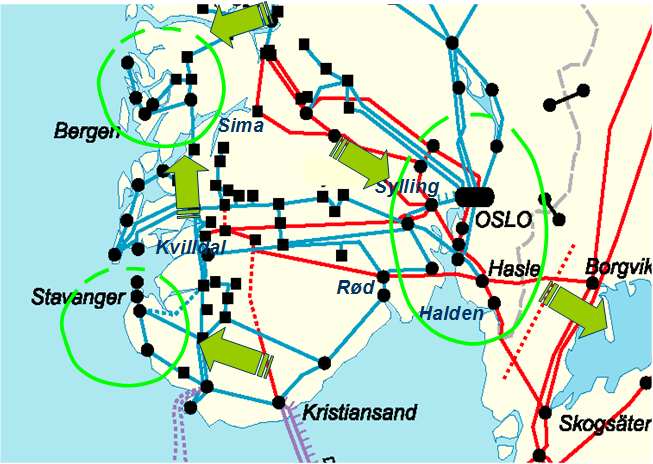
\includegraphics[width=1\textwidth]{Figs/Hasle.png}    
\end{column}
\begin{column}{0.5\textwidth}
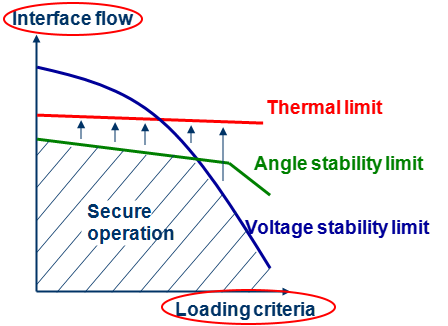
\includegraphics[width=1\textwidth]{Figs/SecurityLimits_emphasis.png}
\end{column}
\end{columns}  
\end{frame}


\section{History}

\begin{frame}
  \frametitle{History}
\textbf{January 1989}, EPRI, “Proceedings: Bulk Power System Voltage Phenomena - Voltage Stability and Security.”
  \begin{quote}
    Over the past decade, voltage instability has initiated several severe power system disruptions. Such incidents are likely to increase with increases in transmission line loadings. However, no theoretical or practical body of knowledge is available to meet the needs of power system planners and operators
  \end{quote}
\end{frame}

\begin{frame}
  \frametitle{History, cont.}
Add some historical blackouts.
\end{frame}

\begin{frame}
  \frametitle{History, cont.}
  \begin{itemize}
  \item \textbf{September 1989}: Dobson and Chiang, “Towards a Theory of Voltage Collapse in Electric Power Systems.”
  \item \textbf{October 1989}: Ajjarapu and Christy, “The Application of a Locally Parameterized Continuation Technique to the Study of Steady State Voltage Stability.”
  \item \textbf{1992}: Ajjarapu and Christy, “The Continuation Power Flow: A Tool for Steady State Voltage Stability Analysis.”
  \item \textbf{1992}: Dobson and Lu, “Voltage Collapse Precipitated by the Immediate Change in Stability When Generator Reactive Power Limits Are Encountered.”
  \item \textbf{1998}: Van Cutsem and Vournas, Voltage Stability of Electric Power Systems.
  \item \textbf{2007}: Ajjarapu, Computational Techniques for Voltage Stability Assessment and Control.
  \end{itemize}
And many, many other contributors \ldots
\end{frame}


\section[NR method]{Newton-Raphson method}
\label{sec:newt-raphs-meth}


\begin{frame}
  \frametitle{Newton-Raphson method}
  \begin{itemize}
  \item Method to compute $x^{*}$ such that $f(x^{*}) = 0$.
  \item Requires an initial guess.
  \item Relies on a first-order approximation of $f$ around the current guess $x_i$:
    \begin{align}
      f(x) = f(x_i) + \nabla_x f(x_i) (x-x_i) + \text{ higher order term}
    \end{align}
  \end{itemize}
\end{frame}

\begin{frame}
  \frametitle{Newton-Raphson method, algorithm}
  \begin{enumerate}
  \item Set $x_i = x_0$;
  \item \textbf{While} $\norm{f(x_i)}> \epsilon$, \textbf{do}
    \begin{align}
      \label{eq:2}
      x_{i+1} = x_i - \left(\nabla_x f(x_i) \right)^{-1} f(x_i)
    \end{align}
  \item Hope that you guessed $x_0$ right so that the method converges.
  \end{enumerate}
\end{frame}

\section[Power flow]{Power flow computations by Newton-Raphson method}

\begin{frame}
  \frametitle{Power flow computations}
  \begin{itemize}
  \item \textbf{Objective}: \only<1>{?} \only<2->{Find voltage magnitudes and angles at all buses, given power injections, voltage set points and angle references at some buses.}
  \item<3-> \textbf{Method}: Active and reactive power balance at each bus must hold.
    \begin{align}
      \Delta P &= P_g - P_l - P_s(\theta,V) = 0,\\
      \Delta Q &= Q_g - Q_l - Q_s(\theta,V) = 0,
    \end{align}
  \item<4> Can be written
    \begin{align}
      x &= [\theta \; V] \\
      f(x) &= \begin{bmatrix}
      \Delta P(x)\\
      \Delta Q(x)
      \end{bmatrix}=0
    \end{align}
  \end{itemize}
\end{frame}

\begin{frame}[label=nr-power-flow]
  \frametitle{Newton-Raphson iteration for power flows}
The power flow equations $f(x)=0$ can be solved by the Newton-Raphson method. Iterations:
  \begin{align}
      x_{i+1} = [\theta_{i+1} \; V_{i+1}] = x_i - J(x_i)^{-1} f(x_i)
  \end{align}
with ($i$ is for iteration number, \emph{not} bus number)
\begin{align}
  J(x_i) = J([\theta_i \; V_i]) = \begin{bmatrix}
     \frac{\partial \Delta P}{\partial \theta} & \frac{\partial \Delta P}{\partial V} \\
     \frac{\partial \Delta Q}{\partial \theta} & \frac{\partial \Delta Q}{\partial V}
   \end{bmatrix} = \begin{bmatrix}
   f_{\theta} & f_V
   \end{bmatrix}
\end{align}
So why can't we use power flow computations for obtaining the PV curves?\\
\visible<2>{
\begin{enumerate}
\item The Jacobian is singular at the nose point $\Rightarrow$ numerical problems as we get close to this point. 
\item Convergence of NR method very sensitive to initial conditions $\Rightarrow$ can be difficult to get convergence even away from the nose point.
\end{enumerate}
}
\end{frame}

\section[CPF]{Continuation power flow}
\label{sec:cont-power-flow}
\subsection{Parametrizing the loading increase}
\begin{frame}
  \frametitle{Parametrization of load increase}
There is a \alert{loading} point beyond which the system becomes unstable.
How to define a \alert{loading} and a \alert{loading increase} in power systems?
  \begin{itemize}
  \item Add one parameter $\lambda \in \R$ to parametrize the load increase process in direction $d\in \R^n$:
    \begin{align}
      P_l = P_l^0 + \lambda d \in \R^n
    \end{align}
  \item For example, in a three-bus system with two loads at buses 2 and 3, the loads could be increased as follows
    \begin{align}
      P_l =
      \begin{bmatrix}
        0 \\
        150 \\
        120
      \end{bmatrix} + \lambda
      \begin{bmatrix}
        0 \\
        1\\
        1
      \end{bmatrix}
    \end{align}
  \end{itemize}
\end{frame}

\begin{frame}
  \frametitle{Parametrization of load increase, cont.}
  \begin{itemize}
  \item Reactive power: typically, we assume constant power factor load (but the method can handle other models as well), so
    \begin{align}
      Q_l = \text{diag}(\tan \phi) P_l = Q_l^0 + \lambda \cdot \text{diag}(\tan \phi) d 
    \end{align}
  \item Note that $\text{diag} (\tan \phi)$ is simply a square matrix with the $\tan \phi_i$ on the diagonal
  \item For example, with $\tan \phi = Q_0/P_0 = 0.5$ for all loads, 
    \begin{align}
      Q_L =
      \begin{bmatrix}
        0\\
        75\\
        60
      \end{bmatrix} + \lambda
      \begin{bmatrix}
        0\\
        0.5\\
        0.5
      \end{bmatrix}
    \end{align}
  \end{itemize}
\end{frame}

\begin{frame}
  \frametitle{Illustration on the board}
  Two-dimensional load increase from $P_l^0$ in direction $d$.
  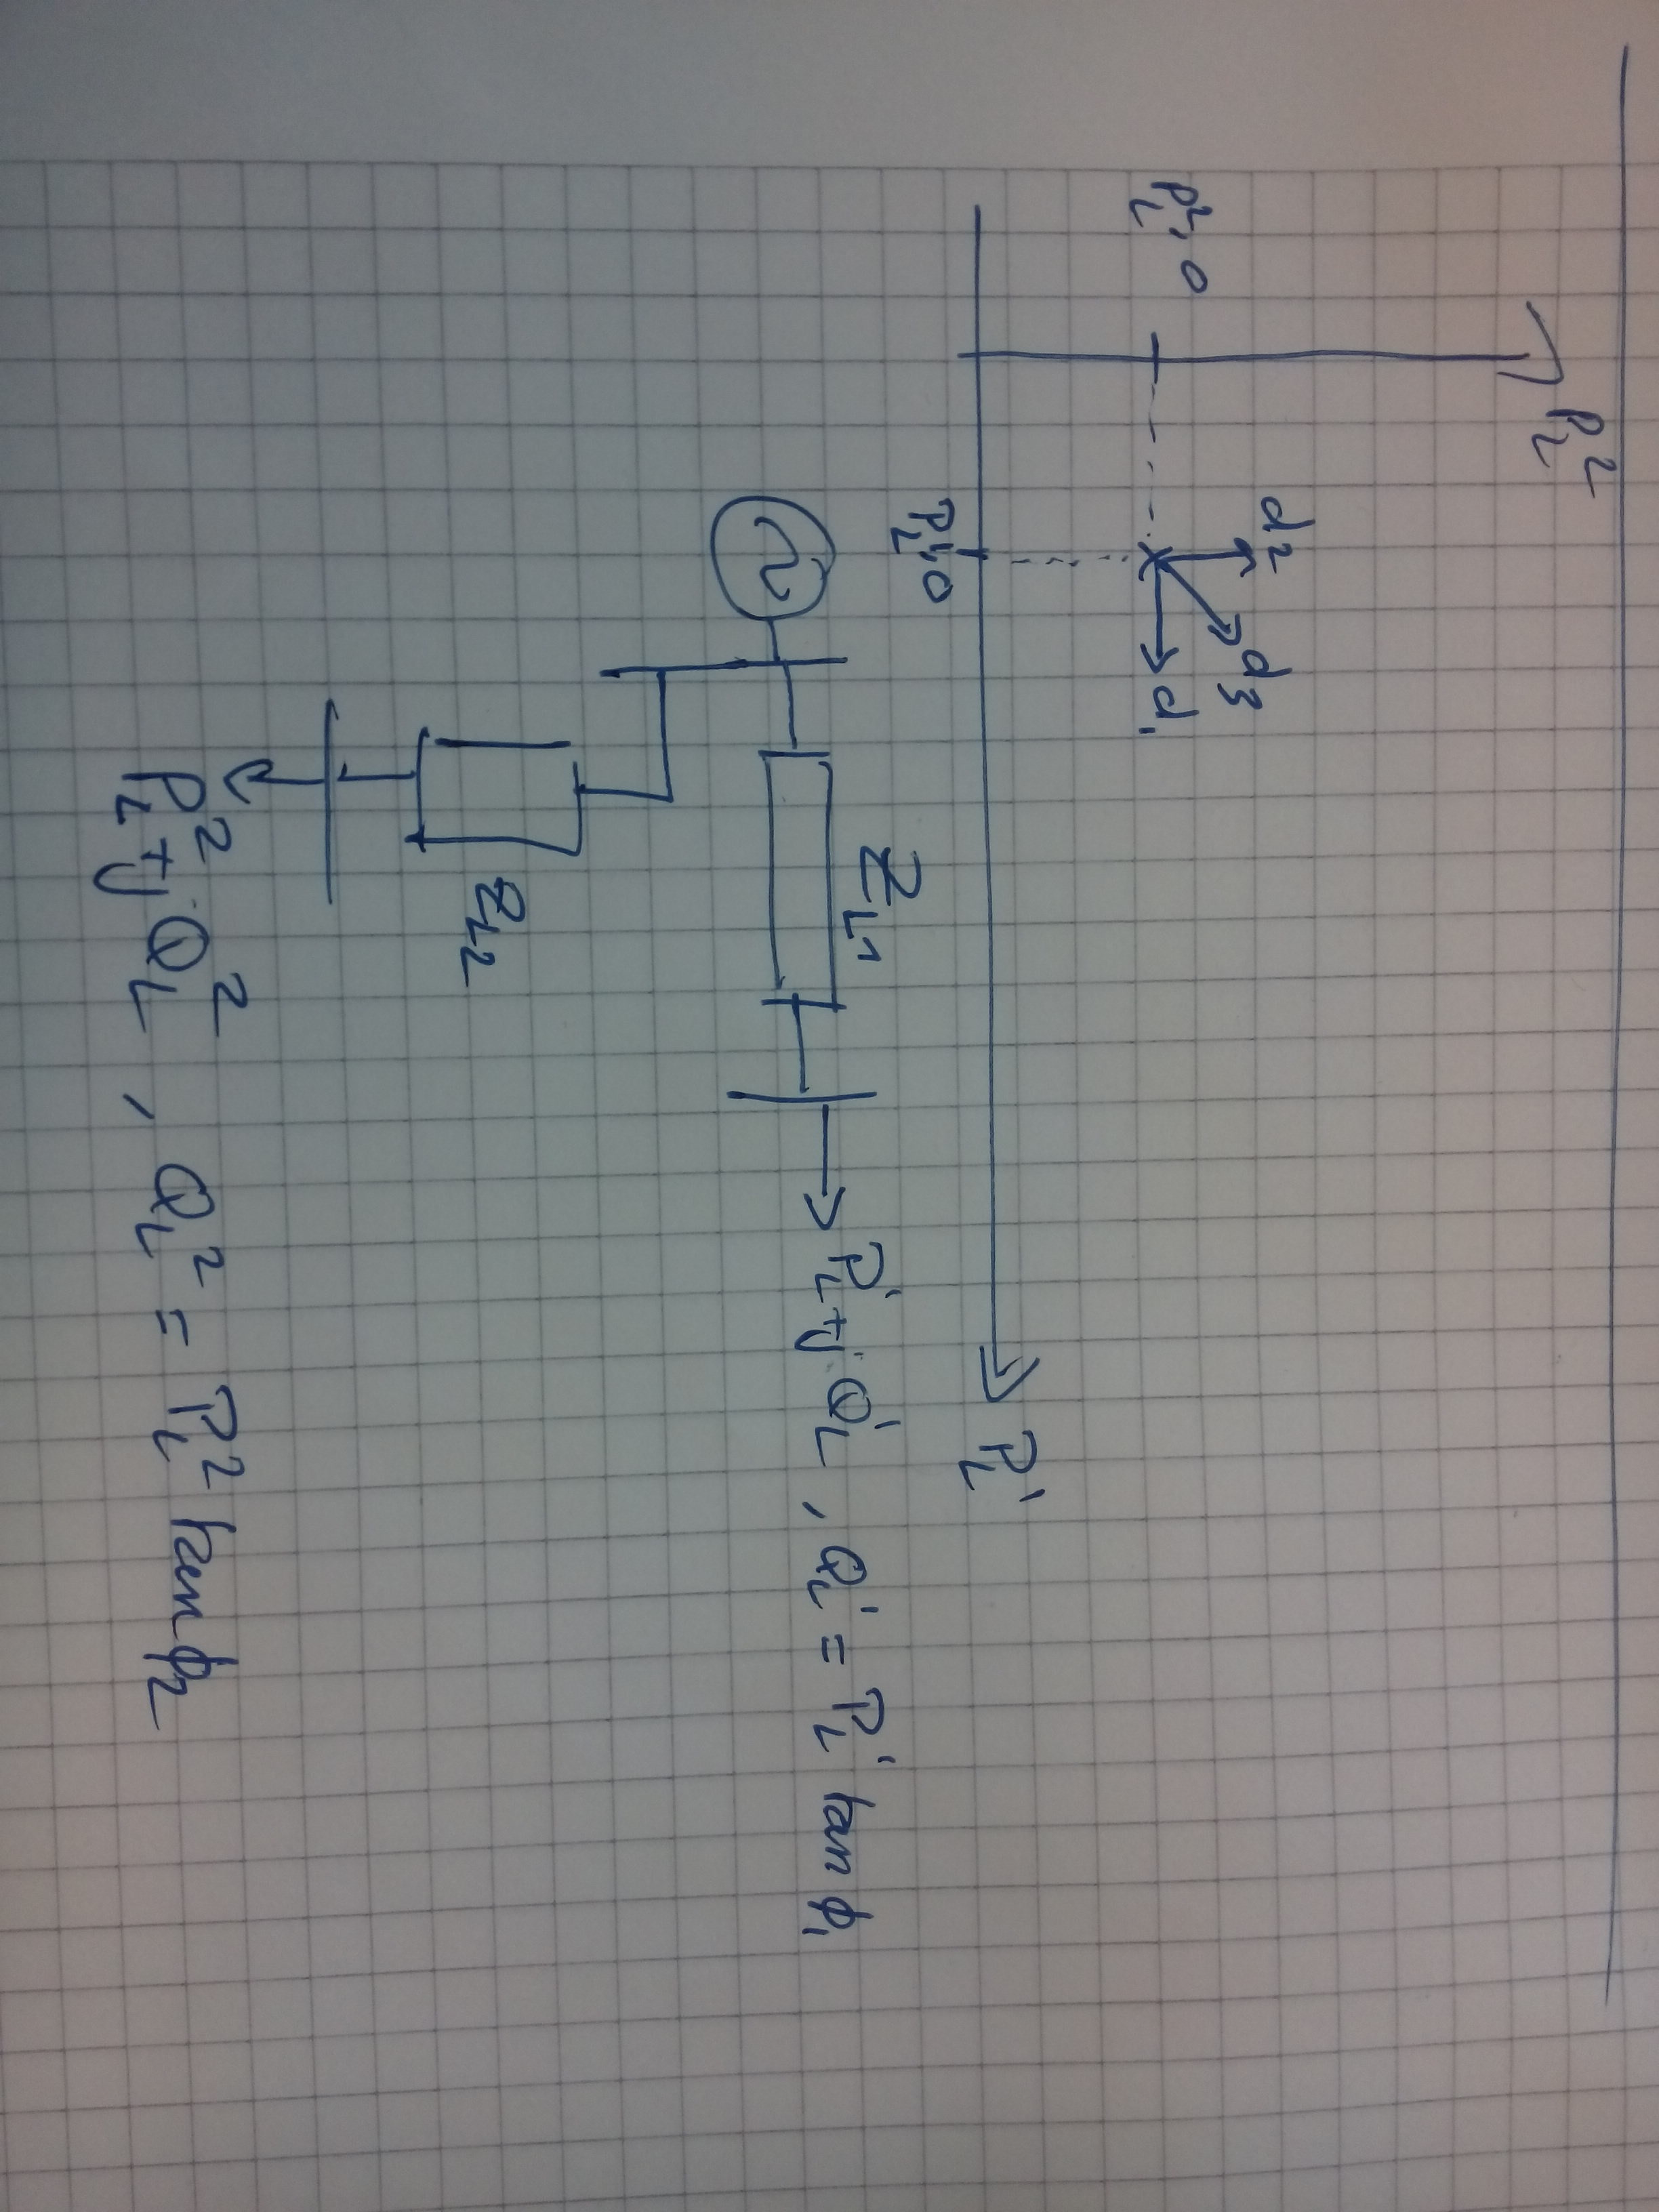
\includegraphics[angle=90,width=0.7\textwidth]{Figs/LoadIncrease.jpg}

\textbf{Note:} Important to keep in mind which space ($V-\lambda$, $P_l$, etc.) is of interest.
\end{frame}

\begin{frame}
  \frametitle{Extending the power flow equations}
\begin{align}
      0 &= P_g^i - P_l^i - P_s^i(\theta,V), \quad \forall \text{ PV and PQ buses} \label{eq:pf-p} \\
      0 &= Q_g^i - Q_l^i - Q_s^i(\theta,V), \quad \forall \text{ PQ buses} \label{eq:pf-q}\\
      P_l &= P_l^0 + \lambda d \in R^n \label{eq:cpf-lambda} \\
      Q_l &= Q_l^0 + \lambda \cdot \text{diag}(\tan \phi) d \label{eq:cpf-lambda-q}
    \end{align}
    \begin{center}
    \begin{tabular}{ccc}
    \toprule
      & PF & CPF \\
    \midrule
    Equations & \eqref{eq:pf-p}, \eqref{eq:pf-q} & \eqref{eq:pf-p}, \eqref{eq:pf-q}, \eqref{eq:cpf-lambda}, \eqref{eq:cpf-lambda-q}\\
    Variables & $x = [\theta \; V]$ & $z = [x \; \lambda] = [\theta \; V \; \lambda]$ \\
    Parameters & $P_l$, $\tan \phi$ & $P_l^0$, $\tan \phi$, $d$, $\lambda$ \\
     & (and $P_g$, $\theta_{\text{slack}}$, \ldots) & (and $P_g$, $\theta_{\text{slack}}$, \ldots) \\
    \bottomrule
    \end{tabular}  
    \end{center}
Increasing $\lambda \Leftrightarrow$ simulating a load increase in direction $d$.
\end{frame}

\subsection{CPF: the thee steps}

\begin{frame}
  \frametitle{CPF: Principles}
The CPF is a predictor-corrector process:
\begin{enumerate}
\item Start from an operating point $z_i = [\theta_i \; V_i \; \lambda_i]$.
\item Predict what the operating point becomes when loading increases in direction $d$ $\Rightarrow$ $z_{i+1}^p$.
\item Correct the prediction to get a real operating point $z_{i+1}$.
\end{enumerate}
\begin{figure}[!h]
  \centering
  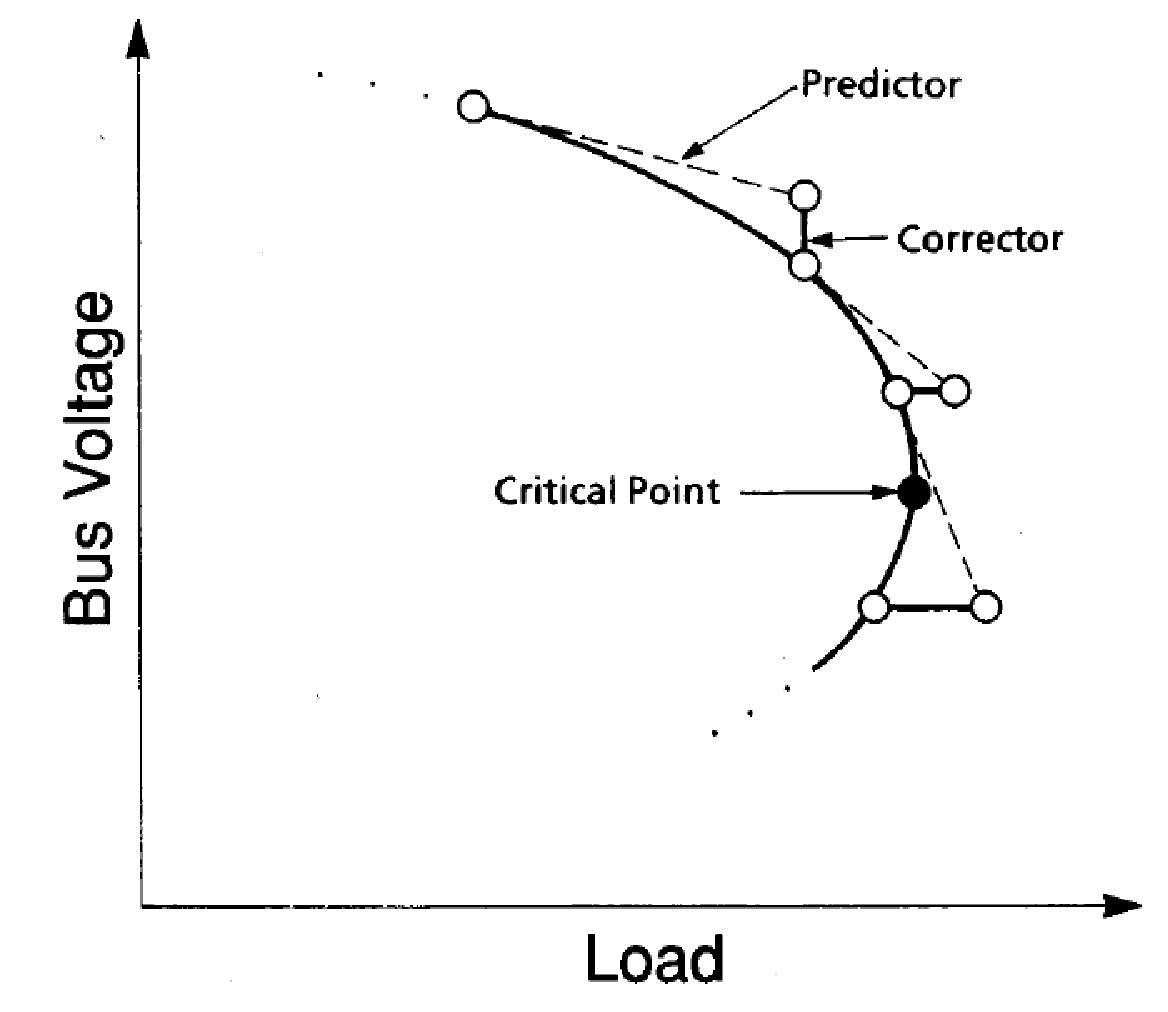
\includegraphics[width=0.4\textwidth]{CPFprocess.pdf}
  \caption{CPF process, from Ajjarapu and Christy, “The Continuation Power Flow: A Tool for Steady State Voltage Stability Analysis.”}
  \label{fig:CPFprocess}
\end{figure}
\end{frame}

\begin{frame}
  \frametitle{Steps in CPF}
Three main steps:
\begin{enumerate}
\item Predictor step: From a known operating point $z_i$ (ex: previously corrected), take a step in the direction of the tangent vector $t_{i}$.
  \begin{align}
  z_{i+1}^p = [\theta_{i+1} \; V_{i+1} \; \lambda_{i+1} ]= z_{i} + s \cdot t_{i}  
  \end{align}
\end{enumerate}
\textbf{Notes:}
\begin{itemize}
\item  The predicted point does not correspond to a physical operating point. 
\item It is a mathematical construction to estimate the values of $z=[\theta \; V \; \lambda]$ after taking a step of length $s$ in direction $d$ (in the load space = $P_l$-space).
\item It gives a good initial guess of $z$ before the corrector step.
\end{itemize}
\end{frame}

\begin{frame}
\frametitle{Steps in CPF, cont.}
  \begin{enumerate}
 \setcounter{enumi}{1}
  \item Choosing the continuation parameter: which component in $z = [\theta \; V \; \lambda]$ should we keep constant in the corrector step?
\item Corrector step: Correct the predicted value to a valid operating point (= ``project'' back onto the PV curve), keeping the continuation parameter constant. Solve:
  \begin{align}
      0 &= P_g - (P_l^0 + \lambda_{i+1} d) - P_s(\theta_{i+1},V_{i+1}),\label{eq:corr-1}  \\
      0 &= Q_g - (Q_l^0 + \lambda_{i+1} \cdot \text{diag}(\tan \phi) d)- Q_s(\theta_{i+1},V_{i+1}), \\
      0 &= z_{i+1}^{k}-z_{i+1}^{k,p} \label{eq:corr-3}
  \end{align}
  Equations \eqref{eq:corr-1}--\eqref{eq:corr-3} solved for $z_{i+1} = [\theta_{i+1} \; V_{i+1} \; \lambda_{i+1}]$ by Newton-Raphson method.
  \end{enumerate}
\textbf{Notes}:
\begin{itemize}
\item Without \eqref{eq:corr-3}, the system of equations is underdetermined.
\item \eqref{eq:corr-3} says how to correct onto the PV curve (keeping $\lambda$ constant, keeping some $V_m$ constant, \ldots)
\end{itemize}
\end{frame}

\begin{frame}
  \frametitle{Illustration on the board}
  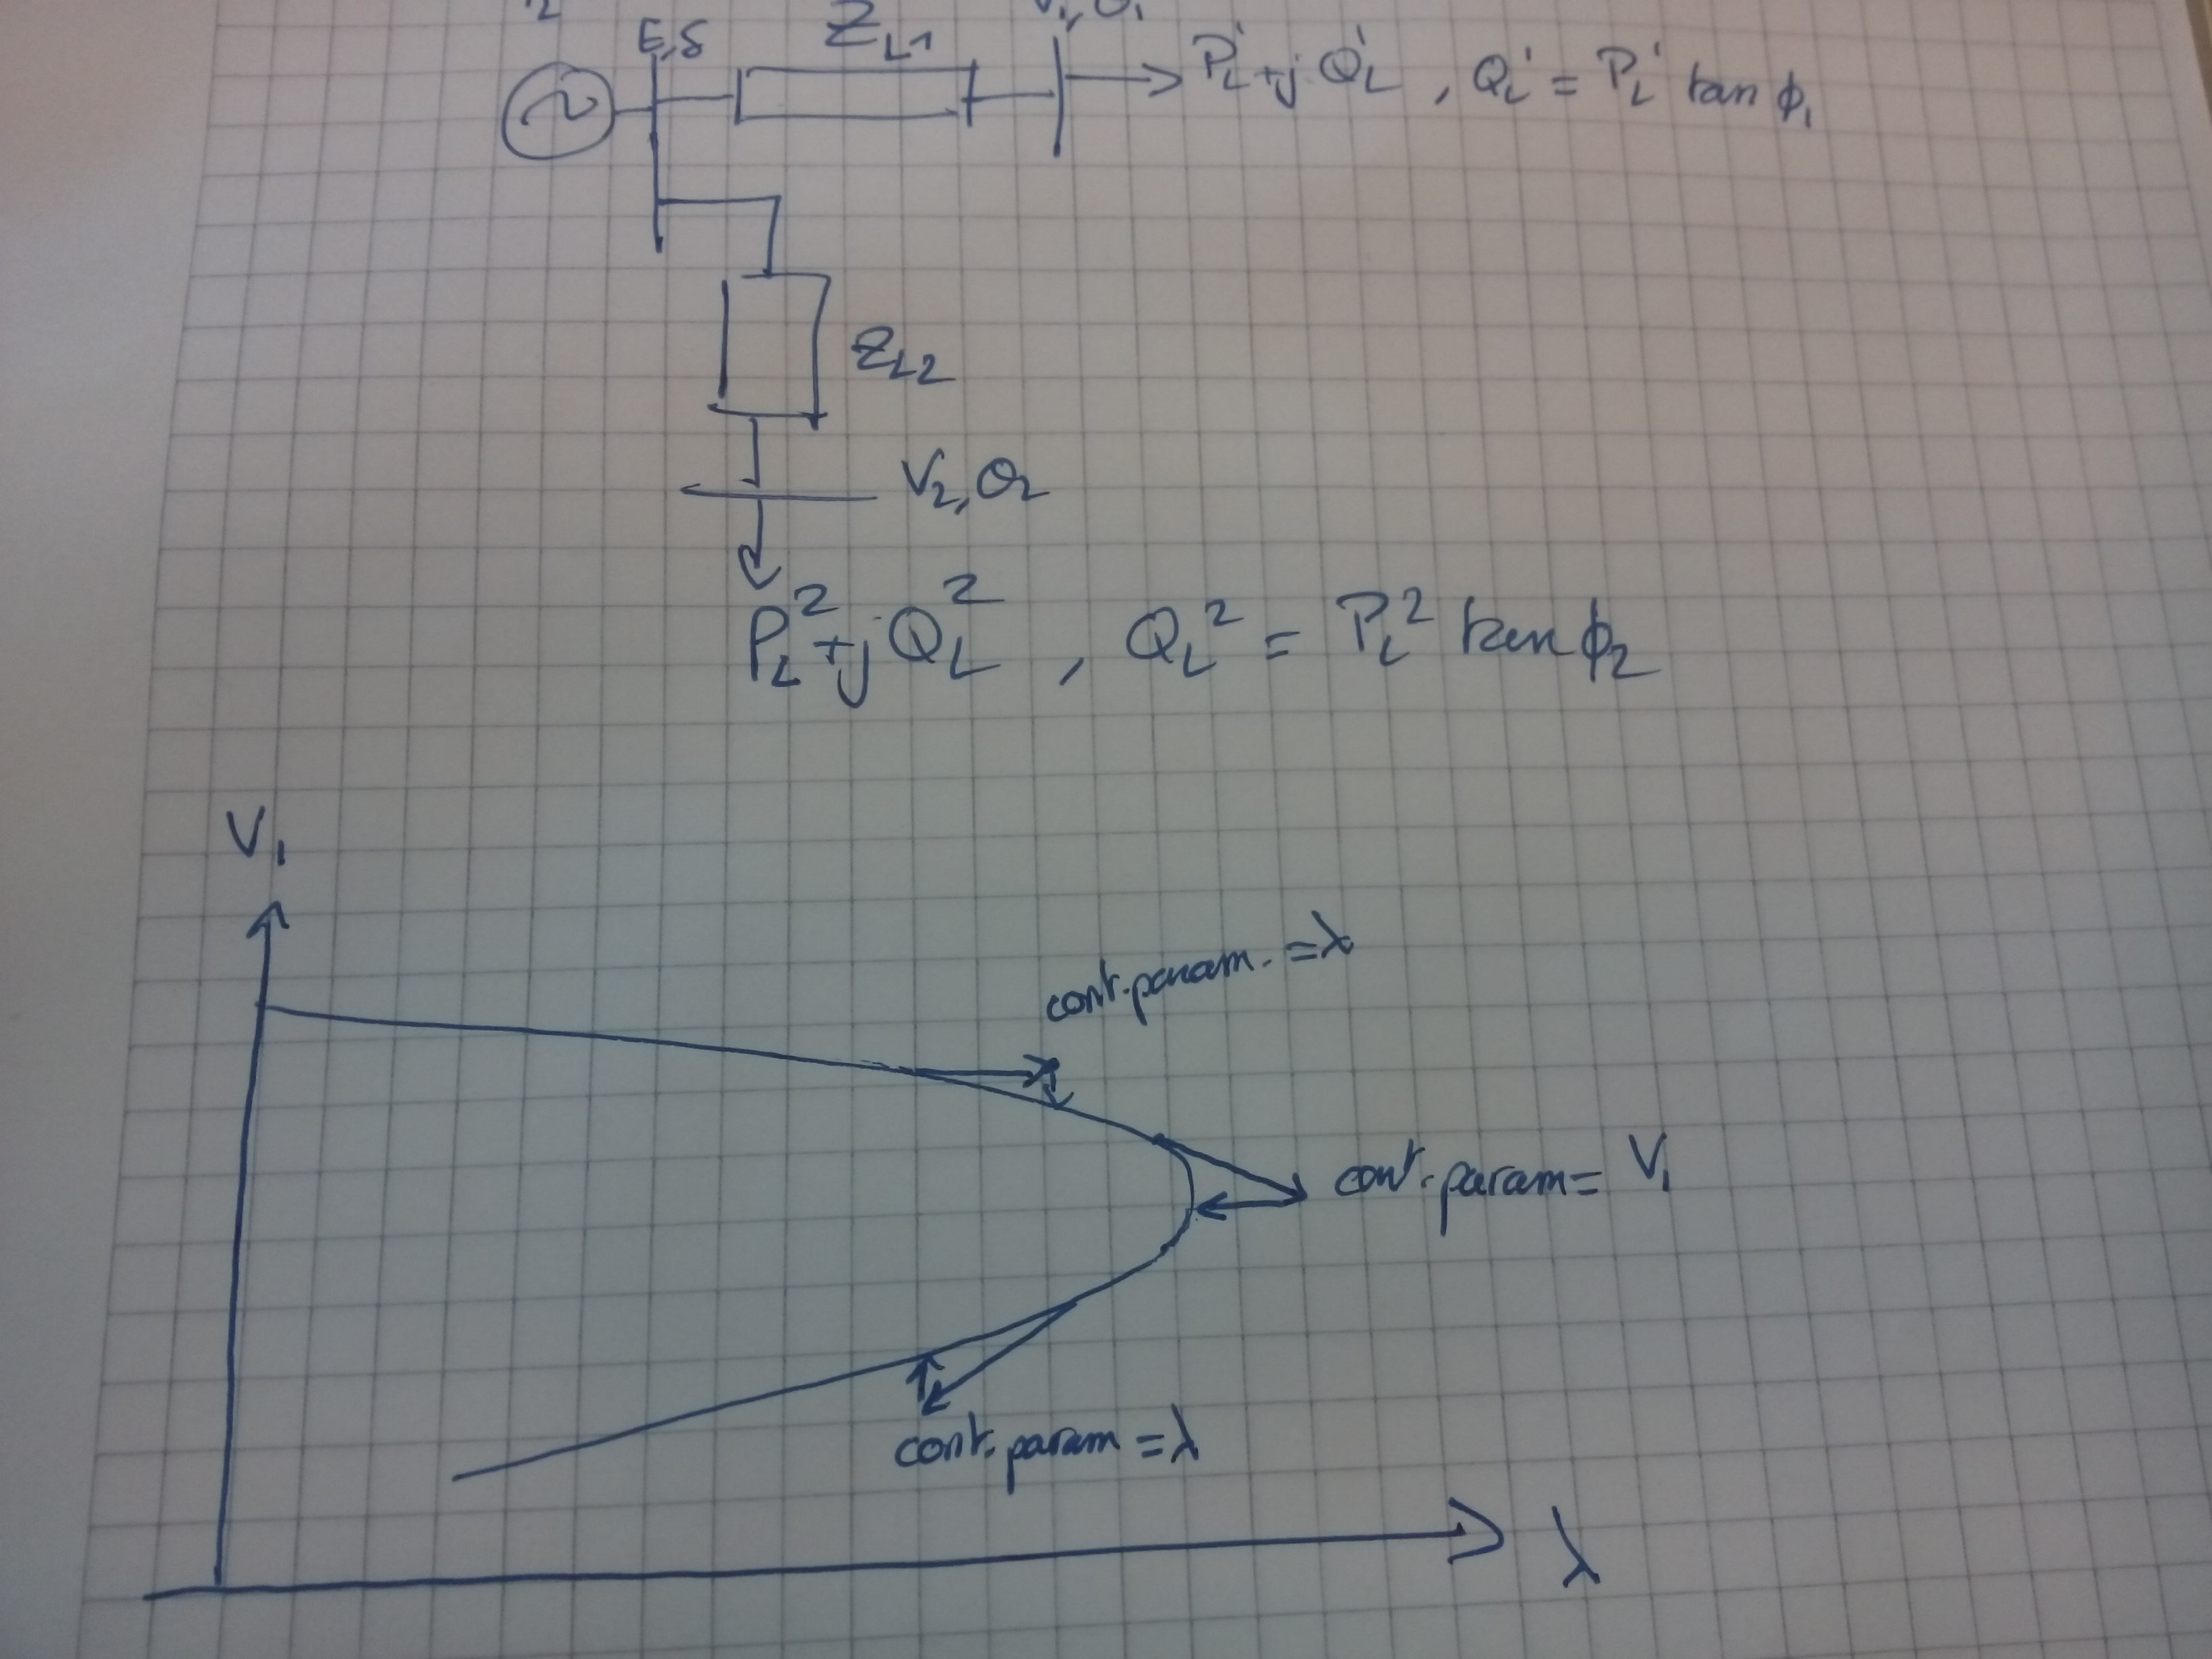
\includegraphics[width=0.7\textwidth]{Figs/CPF_cont_param.jpg}
\end{frame}

\subsection{The three steps in detail}

\begin{frame}
  \frametitle{Predictor step, details}
  From a known operating point $z_i$ (ex: previously corrected), take a step in the direction of the tangent vector $t_{i}$.
  \begin{align}
  z_{i+1}^p = [\theta_{i+1} \; V_{i+1} \; \lambda_{i+1} ]= z_{i} + s \cdot t_{i}  
  \end{align}
\textbf{Question:} How is defined the tangent vector?


\textbf{More general question:} How to compute \emph{one} tangent vector to a surface described by $g(u) = 0$?

\textbf{Notes:}
\begin{itemize}
\item $t_{i}$ is the tangent vector to the operating point $z_i = [\theta_i \; V_i \; \lambda_i]$ defined by the power flow equations $f(z_i) = 0$. 
\item Notice the space we are talking about. It is the $z$-space, not only the $(V,\lambda)$-space
\item Where is the direction $d$ here?
\end{itemize}
\end{frame}

\begin{frame}
  \frametitle{Computing a tangent vector}
  Equation of the form 
  \begin{align}
    \label{eq:4}
    g(u_0) = 0
  \end{align}
Any vector $t$ in the null space of the Jacobian $J(u_0)$ is a tangent vector to $g$ at $u_0$, i.e. any vector $u\neq 0$ such that
\begin{align}
  \label{eq:5}
  J(x_0) t = 0.
\end{align}
Intuition,
\begin{align}
  \label{eq:6}
  g(u_0+t) &= g(u_0) + J(u_0) t + \text{ higher order terms}
\end{align}
The set of all $u_0+t$ such that $J(u_0) t = 0$ is the tangent plane of $g$ at $u_0$.
\vskip0.5cm
\footnotesize See also \url{http://mathworld.wolfram.com/SubmanifoldTangentSpace.html}
\end{frame}

\begin{frame}
  \frametitle{Tangent vector to power flow equations}
  Let $z_i = [\theta_i \; V_i \; \lambda_{i}]$ be an operating point, i.e.
  \begin{align}
    \label{eq:7}
    \Delta P (z_i) &= 0 \\
    \Delta Q (z_i) &= 0
  \end{align}
Any vector $t$ such that
\begin{align}
  \label{eq:tangent-vectors}
  J(z_i)t = \begin{bmatrix}
  \frac{\partial \Delta P}{\partial \theta} & \frac{\partial \Delta P}{\partial V} & \frac{\partial \Delta P}{\partial \lambda} \\
  \frac{\partial \Delta Q}{\partial \theta} & \frac{\partial \Delta Q}{\partial V} & \frac{\partial \Delta Q}{\partial \lambda}
  \end{bmatrix} t = 0
\end{align}
is a tangent vector.

\textbf{Note:} We cannot just solve $J(z_i) t = 0$ for $t$ to find $t$ (i.e. \eqref{eq:tangent-vectors} is a necessary but not sufficient condition to get \emph{the} $t$ we are looking for). Why? \only<2>{Ex: $t$ = 0 satisfies \eqref{eq:tangent-vectors}.}
\end{frame}

\begin{frame}
  \frametitle{Tangent vector to power flow equations, cont.}
  \begin{itemize}
  \item We need one more equation to specify which tangent vector, among all possible satisfying \eqref{eq:tangent-vectors}, we want to obtain.
  \item Typically, we want one component $k$ in $v$ to be equal to one, so 
    \begin{align}
      \label{eq:10}
      t_k = \pm 1
    \end{align}
  \end{itemize}
 Combining everything:
\begin{align}
  \begin{bmatrix}
  \frac{\partial \Delta P}{\partial \theta} & \frac{\partial \Delta P}{\partial V} & \frac{\partial \Delta P}{\partial \lambda} \\
  \frac{\partial \Delta Q}{\partial \theta} & \frac{\partial \Delta Q}{\partial V} & \frac{\partial \Delta Q}{\partial \lambda} \\
   & e_k^T & 
  \end{bmatrix} t = \pm e_{2n+1}
\end{align}
where $e_j$ is the $j$-th column of the identity matrix $I_{2n+1}$.
\end{frame}

\begin{frame}
  \frametitle{Tangent vector, summary}
Combining everything:
\begin{align}
  \label{eq:tangent-vectors-2}
  \begin{bmatrix}
  \frac{\partial \Delta P}{\partial \theta} & \frac{\partial \Delta P}{\partial V} & \frac{\partial \Delta P}{\partial \lambda} \\
  \frac{\partial \Delta Q}{\partial \theta} & \frac{\partial \Delta Q}{\partial V} & \frac{\partial \Delta Q}{\partial \lambda} \\
   & e_k^T & 
  \end{bmatrix} t = Bt = \pm e_{2n+1}
\end{align}
where $e_j$ is the $j$-th column of the identity matrix $I_{2n+1}$, and $B$ is just the matrix on the left.

\textbf{Solving \eqref{eq:tangent-vectors-2}}: Simply use the inverse of matrix on the left: $t = B^{-1} (\pm e_{2n+1})$.

\textbf{Interpretation:} By following $t$, the $k$-th component in $z$ changes with 1 or -1, the other ones change with $t_j$, $j \neq k$, where these $t_j$ are computed from \eqref{eq:tangent-vectors-2} to make sure that the step we take is in the tangent plane around the current operating point $z_i$.

\textbf{Question:} Where is the direction $d$?  
\end{frame}

\begin{frame}
  \frametitle{Tangent vector, example}
  Matlab example.
\end{frame}

\begin{frame}
  \frametitle{Choosing the continuation parameter}
  \begin{itemize}
  \item Previously: predictor step gave $t$ and $z_{i+1}^p = z_i + s \cdot t$
  \item Problem: $z_{i+1}^p$ does not satisfy power flow equations (it satisfies them only to the first order, in fact).
  \item Now: correct the prediction to get an operating point satisfying the power flow equations.
\item Remember, in the next step, the correction step, some component of $z=[\theta \; V \; \lambda]$ will be kept constant:
\begin{align}
      0 &= P_g - (P_l^0 + \lambda_{i+1} d) - P_s(\theta_{i+1},V_{i+1}),\\
      0 &= Q_g - (Q_l^0 + \lambda_{i+1} \cdot \text{diag}(\tan \phi) d)- Q_s(\theta_{i+1},V_{i+1}), \\
      0 &= z_{i+1}^{k}-z_{i+1}^{k,p} \label{eq:corr-param}
\end{align}
  \end{itemize}
\textbf{Intuition:}
\begin{itemize}
\item we want to have control over the component that varies the fastest when taking a step.
\item How to choose among all $\theta$, $V$ and $\lambda$ the one we want to keep constant?
\item Hints: it is related to the tangent vector $t$.
\end{itemize}
\end{frame}

\begin{frame}
  \frametitle{Choosing the continuation parameter, cont.}
\begin{align}
  \begin{bmatrix}
  \frac{\partial \Delta P}{\partial \theta} & \frac{\partial \Delta P}{\partial V} & \frac{\partial \Delta P}{\partial \lambda} \\
  \frac{\partial \Delta Q}{\partial \theta} & \frac{\partial \Delta Q}{\partial V} & \frac{\partial \Delta Q}{\partial \lambda} \\
   & e_k^T & 
  \end{bmatrix} t = \pm e_{2n+1}
\end{align}
  \begin{itemize}
  \item Remember: Each component in $t$ is associated with either one bus voltage angle $\theta_j$, one bus voltage magnitude $V_j$ or the loading $\lambda$.
  \item The components in the tangent vector $t$ indicates how all variables $\theta$, $V$ and $\lambda$ vary when we take a step.
  \item We choose $k$ corresponding to the component with maximum variation:
    \begin{align}
      \label{eq:1}
      k = \argmax \{|t_1|,\ldots,|t_{2n+1}|\}
    \end{align}
  \end{itemize}
\end{frame}

\begin{frame}
  \frametitle{Correction step, details}
  \begin{itemize}
  \item Previously:
    \begin{enumerate}
    \item $z_{i+1}^p$: predicted value = approximation of the operating point when taking a step from $z_i$ in direction $p$.
    \item $k$: the variable, among all $\theta$, $V$ and $\lambda$, that is kept constant during the correction step.
    \end{enumerate}
  \item Corrector step ``easy'': we just need to solve:
\begin{align}
      0 &= P_g - (P_l^0 + \lambda_{i+1} d) - P_s(\theta_{i+1},V_{i+1}),\\
      0 &= Q_g - (Q_l^0 + \lambda_{i+1} \cdot \text{diag}(\tan \phi) d)- Q_s(\theta_{i+1},V_{i+1}), \\
      0 &= z_{i+1}^{k}-z_{i+1}^{k,p}
\end{align}
\textbf{Question:} How to solve this? \only<2>{using Newton-Raphson method}
  \end{itemize}
\end{frame}

\begin{frame}
  \frametitle{Corrector step with Newton-Raphson}
\begin{align}
      0 &= P_g - (P_l^0 + \lambda_{i+1} d) - P_s(\theta_{i+1},V_{i+1}), \label{eq:corr-eq-1}\\
      0 &= Q_g - (Q_l^0 + \lambda_{i+1} \cdot \text{diag}(\tan \phi) d)- Q_s(\theta_{i+1},V_{i+1}), \\
      0 &= z_{i+1}^{k,p} - z_{i+1}^{k} \label{eq:corr-eq-3}
\end{align}
\begin{itemize}
\item Newton-Raphson with $z_{i+1}^p$ as initial guess
\item $j$-th iteration in Newton-Raphson:
\begin{align}
  \label{eq:3}
  z_{i+1,j+1} = - J_\text{aug}(z_{i+1,j})^{-1} f(z_{i+1,j})
\end{align}
where the Jacobian of \eqref{eq:corr-eq-1}--\eqref{eq:corr-eq-3} is
\begin{align}
  \label{eq:8}
  J_\text{aug}(z_{i+1,j}) = \begin{bmatrix}
  \frac{\partial \Delta P}{\partial \theta} & \frac{\partial \Delta P}{\partial V} & \frac{\partial \Delta P}{\partial \lambda} \\
  \frac{\partial \Delta Q}{\partial \theta} & \frac{\partial \Delta Q}{\partial V} & \frac{\partial \Delta Q}{\partial \lambda} \\
   & e_k^T & 
  \end{bmatrix}
\end{align}
\end{itemize}
\textbf{Note:} Easy to mix up all indices ($i$,$k$,$j$)!
\end{frame}

\subsection{Problems addressed by CPF}

\begin{frame}
  \frametitle{Around the nose point}
Remember: the maximum loadability point is characterized by singularity of the power flow Jacobian $J$ (i.e. $\det J = 0$):
\begin{align}
  \label{eq:9}
  J = \begin{bmatrix}
  \frac{\partial \Delta P}{\partial \theta} & \frac{\partial \Delta P}{\partial V} \\
  \frac{\partial \Delta Q}{\partial \theta} & \frac{\partial \Delta Q}{\partial V}
  \end{bmatrix}
\end{align}
Note that the Jacobian in the corrector process is
\begin{align}
  \label{eq:9}
  J_\text{aug} = \begin{bmatrix}
  \begin{matrix} \vphantom{\begin{matrix} 0 \\ 0 \end{matrix}} 
  J 
 \end{matrix} & \begin{matrix} \frac{\partial \Delta P}{\partial \lambda_i} \\
  \frac{\partial \Delta Q}{\partial \lambda}
  \end{matrix} \\
   & e_k^T & 
  \end{bmatrix}
\end{align}
If we choose $\lambda$ as the continuation parameter, $\det J_\text{aug} = \det J$.
Close to the nose point, $J_\text{aug}$ would also be close to singular.
\end{frame}

\begin{frame}
  \frametitle{Importance of the continuation parameter}
  The continuation parameter helps in two different ways
  \begin{enumerate}
  \item Predictor step: $t_k = \pm 1$ helps controlling the fastest changing variable when we take a step.
  \item Corrector step: Choosing another continuation parameter than $\lambda$ ensures that the corrector step is numerically stable (Jacobian in the Newton-Raphson process not close to singular)
  \end{enumerate}
\end{frame}

\begin{frame}
\frametitle{Why does it help?}
So, why does it help?

Remember, problems with using PF calculations to trace the PV curve:
\begin{enumerate}
\item PF convergence very sensitive to initial conditions $\Rightarrow$ CPF uses a predictor step to get a good initial (=predicted) value.
\item The PF Jacobian is singular at the nose point $\Rightarrow$ numerical problems as we get close to this point $\Rightarrow$ Continuation parameter is set to ensure nonsingularity of the Jacobian matrix.
\end{enumerate}
\end{frame}

\section{Extras}

\begin{frame}
  \frametitle{Demo}
  Matlab demo.
\end{frame}

\begin{frame}
  \frametitle{What we haven't talked about}
  \begin{itemize}
  \item Reactive power limits.
  \item How to choose the step size $s$.
  \item How to interpret and use the tangent vector.
  \item Other load models.
  \item Incorporating load dynamics, generator dynamics, etc
  \end{itemize}
\end{frame}

\begin{frame}
  \frametitle{Inspiration}
  \begin{itemize}
  \item Voltage stability phenomena explained by bifurcation theory (dynamical system). Nose point = saddle-node bifurcation.
  \item Continuation methods come from that field.
  \item Applied by Werner Rheinboldt in the field of structural mechanics.
  \item The work of Rheinboldt inspired Ajjarapu and Christy to adapt the method to the study of voltage stability.
  \end{itemize}
\end{frame}

\begin{frame}
  \frametitle{Take-home messages}
  \begin{itemize}
  \item Understand the Newton-Raphson method and how to use it.
  \item The principles of and intuition behind CPF are simple.
  \item The maths are important. Link intuition to maths! Important to be able to write down intuitions as mathematical formulations.
  \item Keep track of what has a physical meaning and what is just math (predictor step, for example, is a mathematical construction, although the tangent vector does have a physical interpretation)
  \item Keep track of indices, variables, Jacobians \ldots Easy to get lost!
  \item Always make sure you understand the physics (i.e. what are we talking about, what is going on in the system, what is reactive power, \ldots)
  \item When encountering a new problem, study other fields.
  \end{itemize}
\end{frame}

\end{document}

%%% Local Variables:
%%% mode: latex
%%% TeX-master: t
%%% End:
